\clearpage
\bookpart{随机采样与积分计算}{Random Sampling and Integration}
\label{part:sampling-and-integration}

\BookPartGuide{%
高维积分往往没有公式，网格求积的点数又随维数爆炸增长。用随机样本求平均是另一条路：误差按样本数的平方根缩小，与维数没有直接关系。要走通这条路，需要能生成给定分布的样本，并且知道误差有多大、怎样减小。

第~\ref{chap:sample-generation}章从均匀随机数出发，用变量变换、分步生成、拒绝筛选构造目标分布的样本，并构造以目标分布为不变分布的 Markov 链。第~\ref{chap:monte-carlo-integration-error}章分析用样本平均估计积分的误差，包括近似生成和样本相关带来的影响。第~\ref{chap:variance-reduction}章从改变分布、改变计算公式和改变抽样机制三个方向减小估计的方差。

第~\ref{chap:expectation-gradient-estimation}章研究分布或被积函数含参数时期望的导数怎样用样本估计。第~\ref{chap:sampling-budget-method-selection}章在给定精度和预算时，比较并组合前面的方法，确定样本的分配与停止的依据。}

\chapter{采样生成}
\label{chap:sample-generation}

计算机能直接给出的随机量只有一种：一串近似独立、近似均匀分布在$(0,1)$上的数。可是要计算的往往是另一个分布下的量，例如指数分布的等待时间、两个高斯成分的混合、只知道到一个常数因子的密度$\widetilde{p}(x)\propto\mathrm{e}^{-U(x)}$。怎样把均匀数加工成这些分布的样本？加工出来的东西是不是真的服从目标分布，彼此是否独立，又要花多少计算？

本章分两条路回答。第一条路是直接生成：把均匀数代入一个确定的映射（变量变换），或者分几步依次抽取（分步生成），或者先多抽一些候选再按比例筛掉一部分（拒绝采样）。只要每次都用新的均匀数从头做起，得到的就是相互独立、服从目标分布的样本。第二条路用于直接生成做不到的情形：构造一个在状态之间游走的Markov链，使目标分布在一步更新下保持不变，链在目标概率大的地方停留更久。这样得到的状态序列通常是相关的，它是否以及多快地“走遍”目标，需要另外的条件。

第~\ref{sec:sgen-uniform}节说明均匀数这一输入的数学模型和计算机实现之间的差别。第~\ref{sec:sgen-transform}节到第~\ref{sec:sgen-rejection}节依次讲三种直接生成，第~\ref{sec:sgen-mcmc}节构造链式更新，第~\ref{sec:sgen-checks}节讨论怎样核对生成结果。全章用两个例子贯穿：$\{1,2,3\}$上质量为$(0.2,0.5,0.3)$的离散分布，以及混合分布$0.3\,\mathcal{N}(-2,0.5^{2})+0.7\,\mathcal{N}(2,1)$。手算时固定使用几个均匀随机数，例如$u=0.37$、$u=0.80$，读者可以逐步复现。

\section{基础随机数}
\label{sec:sgen-uniform}

一切生成方法都从同一种原料出发。把这种原料说清楚，才能说清一种方法“用了多少随机性”“哪些量必须彼此独立”，以及计算机里的随机数在什么意义上可以当作这种原料。

\paragraph{理想模型}
数学上，我们假定能得到一列\term{基础随机数}（basic random numbers）$U_1,U_2,\dots$，它们相互独立，都服从$\operatorname{Unif}(0,1)$。第~\ref{chap:probability-spaces}章在木棍模型$[0,1)$上构造过这样的序列：把一个均匀点的二进制数字交错分组，就得到无穷多个相互独立的均匀变量。所以“有一列独立均匀数”与“有一个均匀数”在数学上是同一个假设，后面不再区分。

一种生成方法就是一个确定的规则$G$：读入若干个基础随机数，输出目标空间中的一点$X=G(U_1,\dots,U_k)$。输出的分布是$(U_1,\dots,U_k)$的均匀分布在$G$下的推前，所以“方法正确”的含义很明确：对目标空间中的每个事件$A$，
\begin{equation}
  \mathbb{P}\bigl(G(U_1,\dots,U_k)\in A\bigr)=\pi(A),
  \label{eq:sgen-correct-law}
\end{equation}
其中$\pi$是目标分布。有些方法读入的个数$k$本身是随机的，例如后面的拒绝筛选要试到成功为止；这时$G$从序列中按顺序取数，读多少由已经读到的数决定，式~\eqref{eq:sgen-correct-law}仍是正确性的定义。

\paragraph{用量与独立性}
评价一种方法时要问两件事。第一件是用量：生成一个样本平均要读入多少个基础随机数，这决定了随机数生成本身的成本。第二件是独立性：哪些步骤必须使用互不重叠的基础随机数。依据是第~\ref{chap:probability-spaces}章的结论：相互独立的随机变量分成互不相交的组，各组的函数仍相互独立。

由此得到重复生成的基本规则。若第$i$个样本只使用第$i$组基础随机数，各组互不重叠，那么
\[
  X_i=G(U_{i,1},\dots,U_{i,k}),\qquad i=1,2,\dots,n
\]
相互独立；若每个$X_i$还满足式~\eqref{eq:sgen-correct-law}，它们就是目标分布的独立同分布样本。反过来，两个样本若共用了某个基础随机数，一般就不再独立。一个样本内部各步骤也是如此：证明一个多步方法正确时，常常要用到“这一步的输入与上一步的输出独立”，这要求两步不共用随机数。第~\ref{sec:sgen-sequential}节会给出一个违反这条规则而出错的例子。

\paragraph{伪随机数}
计算机不能真正产生上述理想序列。它给出的是\term{伪随机数}（pseudorandom numbers）：从一个初始状态$s_0$出发，按确定的递推$s_{k+1}=T(s_k)$更新内部状态，再输出$u_k=g(s_k)\in[0,1)$。初始状态$s_0$称为\term{种子}（seed）。整个序列由种子完全决定，只是在统计性质上模仿独立均匀序列。

最简单的例子是线性同余递推
\begin{equation}
  s_{k+1}=(a\,s_k+c)\bmod m,\qquad u_k=\frac{s_k}{m},
  \label{eq:sgen-lcg}
\end{equation}
其中$a,c,m$是固定的整数。取$m=16$、$a=5$、$c=3$、$s_0=7$，逐项计算：$s_1=(35+3)\bmod16=6$，$s_2=(30+3)\bmod16=1$，依此类推，得到
\[
  7,\ 6,\ 1,\ 8,\ 11,\ 10,\ 5,\ 12,\ 15,\ 14,\ 9,\ 0,\ 3,\ 2,\ 13,\ 4,\ 7,\ \dots
\]
第$16$步回到$7$，此后完全重复。对应的$u_k$依次是$0.4375,\ 0.375,\ 0.0625,\dots$，全都是$1/16$的整数倍。

这个小例子暴露了伪随机数与理想模型的三处差别。第一，序列有周期，状态只有$m$个，最多$m$步后必然重复。第二，取值只在一个有限格点上。第三，相邻的数之间有确定的关系。图~\ref{fig:sgen-lcg-pairs}(a)用$m=256$、$a=5$、$c=1$的递推把相邻两数$(u_k,u_{k+1})$画成平面上的点：由式~\eqref{eq:sgen-lcg}，$u_{k+1}=(5u_k+1/256)\bmod1$，所以全部点落在斜率为$5$的五条线段上，单看每个$u_k$却在$[0,1)$上分布得非常均匀。图~\ref{fig:sgen-lcg-pairs}(b)是现代生成器给出的$256$对数，看不出这种结构。

\begin{BookInlineFigure}
  \centering
  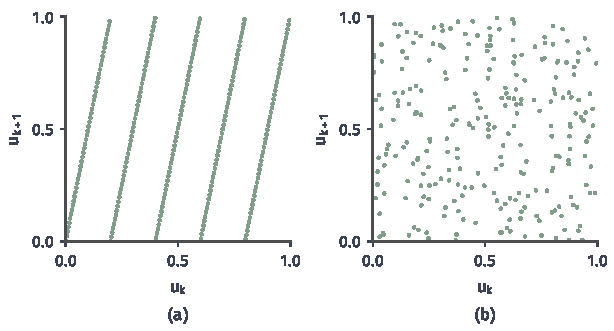
\includegraphics[width=104mm]{figures/07-probability/08-sampling-and-integration/matplotlib/sgen-lcg-pairs/figure.pdf}
  \caption{相邻伪随机数$(u_k,u_{k+1})$组成的点。(a)线性同余递推$s_{k+1}=(5s_k+1)\bmod256$，种子$s_0=7$，一个完整周期的$256$个点全部落在斜率为$5$的五条线段上；(b)NumPy的PCG64生成器，种子$7$，$256$对数。两者的单个$u_k$都在$[0,1)$上均匀分布，差别只在相邻数的联合分布上。}
  \label{fig:sgen-lcg-pairs}
\end{BookInlineFigure}

实用的生成器周期极长（例如$2^{128}$量级），并通过了大量针对相邻数、长程相关和高维分布的统计检验\scite{math-knuth1997seminumerical}。检验通过只说明没有发现所测试的那类偏差，并不证明序列与理想模型无法区分。本卷此后的推导都在理想模型下进行，把“伪随机数足够接近理想模型”当作一个外部假设。

\paragraph{种子与复现}
固定种子，同一程序就产生同一串数，整个计算可以逐位复现。这对查错和比较方法很有用：改动一处代码后用同一种子重跑，结果的变化只来自改动本身。本卷图中的模拟都注明了种子。

复现不等于验证。一个错误的生成方法在固定种子下同样给出可复现的错误结果；某个种子下直方图“看起来对”，换一个种子也可能仍然看起来对，因为错误可能只出现在很少被抽到的区域。生成方法是否正确，要靠式~\eqref{eq:sgen-correct-law}那样的证明，再加上第~\ref{sec:sgen-checks}节的检查；种子只负责让计算可以重来一遍。

\paragraph{有限精度}
浮点数格式也会改变理想模型。常见的双精度均匀数取值于$\{k2^{-53}:k=0,1,\dots,2^{53}-1\}$，可能取到$0$，取不到$1$。若后续要计算$\ln u$，取到$0$就会出错，所以要先确认生成器的取值范围，必要时改用$1-u$。格点还截断了尾部：由$-\ln(1-u)$生成的指数样本不会超过$53\ln2\approx36.7$。对指数分布，被截去的概率约为$\mathrm{e}^{-36.7}$，可以忽略；对尾部很重的分布或专门研究稀有事件的计算，这种截断就需要单独检查。

\section{变量变换构造}
\label{sec:sgen-transform}

最直接的生成方式是找一个确定的映射$T$，把一个容易抽取的变量$V$（通常是若干个基础随机数）变成目标样本$X=T(V)$。这一步本身没有随机性，所有随机性都来自$V$。要说明它正确，就是要算出$T(V)$的分布并与目标比较。

\paragraph{输出分布的两种算法}
$T(V)$的分布是$V$的分布在$T$下的推前：对目标空间的事件$A$，
\[
  \mathbb{P}\bigl(T(V)\in A\bigr)=\mathbb{P}\bigl(V\in T^{-1}(A)\bigr).
\]
这是第~\ref{chap:probability-spaces}章的原像规则，它对任何可测映射成立，不要求$T$可逆，也不要求输出有密度。另一种算法是第~\ref{chap:random-variable-transformations}章的换元公式：若$V$在开集$D\subset\mathbb{R}^{d}$上有密度$f_V$，$T$把$D$一一地映到$T(D)$，连续可微且Jacobian行列式处处非零，记逆映射为$h=T^{-1}$，则$X$有密度
\begin{equation}
  f_X(x)=f_V\bigl(h(x)\bigr)\,\bigl\lvert\det Dh(x)\bigr\rvert,\qquad x\in T(D),
  \label{eq:sgen-change-of-variables}
\end{equation}
在$T(D)$之外为零。换元公式把“质量守恒”写成密度的形式：$x$附近的小体积元来自$h(x)$附近的体积元，体积按$\lvert\det Dh\rvert$倍伸缩，密度按反比变化。

\paragraph{一个用换元公式验证的例子}
取两个独立的基础随机数$(U_1,U_2)$，令
\begin{equation}
  Z_1=\sqrt{-2\ln U_1}\,\cos(2\pi U_2),\qquad Z_2=\sqrt{-2\ln U_1}\,\sin(2\pi U_2).
  \label{eq:sgen-box-muller}
\end{equation}
这称为\term{Box--Muller变换}（Box--Muller transform）。它的想法来自第~\ref{chap:random-variable-transformations}章的极坐标计算：二维标准高斯向量的半径与角度独立，角度均匀，半径平方服从$\operatorname{Exp}(1/2)$。式~\eqref{eq:sgen-box-muller}把$U_2$变成均匀角度$2\pi U_2$，把$U_1$变成半径$R=\sqrt{-2\ln U_1}$。半径平方的分布正是所需的指数分布：对$s>0$，
\[
  \mathbb{P}(R^{2}>s)=\mathbb{P}\bigl(U_1<\mathrm{e}^{-s/2}\bigr)=\mathrm{e}^{-s/2}.
\]

下面用式~\eqref{eq:sgen-change-of-variables}直接验证。$T$把正方形$D=(0,1)^{2}$一一地映到平面去掉非负$z_1$半轴后的区域：半径$r=\sqrt{-2\ln u_1}$取遍$(0,\infty)$，角度$\theta=2\pi u_2$取遍$(0,2\pi)$。记$r^{2}=z_1^{2}+z_2^{2}$，$\theta(z)$为$(z_1,z_2)$在$(0,2\pi)$内的极角，逆映射是
\[
  h(z_1,z_2)=\Bigl(\mathrm{e}^{-r^{2}/2},\ \frac{\theta(z)}{2\pi}\Bigr).
\]
第一个分量对$z_1,z_2$的偏导数分别是$-z_1\mathrm{e}^{-r^{2}/2}$与$-z_2\mathrm{e}^{-r^{2}/2}$；由$\partial\theta/\partial z_1=-z_2/r^{2}$、$\partial\theta/\partial z_2=z_1/r^{2}$，第二个分量的偏导数是$-z_2/(2\pi r^{2})$与$z_1/(2\pi r^{2})$。于是
\[
  \det Dh=-z_1\mathrm{e}^{-r^{2}/2}\cdot\frac{z_1}{2\pi r^{2}}-\Bigl(-z_2\mathrm{e}^{-r^{2}/2}\Bigr)\Bigl(-\frac{z_2}{2\pi r^{2}}\Bigr)=-\frac{\mathrm{e}^{-r^{2}/2}}{2\pi}.
\]
$f_V\equiv1$，代入式~\eqref{eq:sgen-change-of-variables}，得到
\[
  f_Z(z_1,z_2)=\frac{1}{2\pi}\mathrm{e}^{-(z_1^{2}+z_2^{2})/2}=\varphi(z_1)\,\varphi(z_2).
\]
被去掉的半轴面积为零，不影响分布。密度分解为两个标准高斯密度的乘积，所以$Z_1,Z_2$独立，都服从$\mathcal{N}(0,1)$。

用$u_1=0.37$、$u_2=0.80$走一遍：
\[
  r=\sqrt{-2\ln0.37}\approx1.4101,\qquad 2\pi u_2=1.6\pi,
\]
于是
\[
  z_1=1.4101\cos(1.6\pi)\approx0.4358,\qquad z_2=1.4101\sin(1.6\pi)\approx-1.3411.
\]

\paragraph{不需要密度的情形}
换元公式只适用于同维、一一、可微的映射。很多生成映射不满足这些条件，这时直接用原像规则。例如$X=\max\{U_1,U_2\}$把二维变成一维，对$0\le x\le1$，
\[
  \mathbb{P}(X\le x)=\mathbb{P}(U_1\le x,\ U_2\le x)=x^{2},
\]
所以$X$的密度是$2x$。又如下一小节的离散生成，输出只取有限个值，根本没有密度；奇异协方差的高斯生成，输出落在一个低维子空间上，在整个空间中也没有密度。这些情形的输出分布照样由推前确定，正确性同样由式~\eqref{eq:sgen-correct-law}检验。

\subsection{逆分位数采样}
\label{sec:sgen-inverse}

一维的目标分布由分布函数$F$完全确定。对一个均匀数$u$，能否找一个点$x$使“$F$在$x$处恰好累积到$u$”？这就是取分位数。第~\ref{chap:random-variables}章定义了分位数函数
\begin{equation}
  Q(u)=\inf\{x\in\mathbb{R}:F(x)\ge u\},\qquad 0<u<1,
  \label{eq:sgen-quantile}
\end{equation}
并证明了对一切实数$x$，$Q(u)\le x$当且仅当$u\le F(x)$。

\paragraph{方法与正确性}
把基础随机数代入分位数函数，令$X=Q(U)$。由上面的等价关系，
\[
  \mathbb{P}(X\le x)=\mathbb{P}\bigl(U\le F(x)\bigr)=F(x),
\]
所以$X$的分布函数就是$F$。第~\ref{chap:random-variables}章与第~\ref{chap:probability-spaces}章已经从两个角度证明了这一结论，这里关心的是怎样把它变成计算。这种方法称为\term{逆变换采样}（inverse transform sampling）。它对一切实值分布成立：离散、连续或二者混合，有没有密度都一样。几何上，在分布函数的图上从纵轴高度$u$水平向右，碰到曲线（或跳跃的竖直段）后竖直落下，落点就是样本。

\paragraph{分位数有解析式}
若$F$连续且严格递增，$Q$就是$F$的反函数，解方程$F(x)=u$即可。指数分布$\operatorname{Exp}(\lambda)$的$F(x)=1-\mathrm{e}^{-\lambda x}$，解得
\begin{equation}
  Q(u)=-\frac{\ln(1-u)}{\lambda}.
  \label{eq:sgen-exp-quantile}
\end{equation}
取$\lambda=2$、$u=0.37$，得到
\[
  x=-\frac{\ln0.63}{2}\approx\frac{0.4620}{2}=0.2310.
\]
因为$1-U$也服从$\operatorname{Unif}(0,1)$，实际计算中常把式~\eqref{eq:sgen-exp-quantile}换成$-\ln U/\lambda$，省去一次减法；这时需要$U$取不到$0$。

\paragraph{离散分布与累计区间}
设$X$取值$x_1<x_2<\dots<x_K$，概率为$p_1,\dots,p_K$。记累计概率$c_0=0$、$c_k=p_1+\dots+p_k$。此时$F$是阶梯函数，由式~\eqref{eq:sgen-quantile}，$Q(u)=x_k$当且仅当$c_{k-1}<u\le c_k$。也就是说，把$(0,1)$按顺序切成长度为$p_1,\dots,p_K$的区间，$u$落进第$k$段就输出$x_k$：
\begin{equation}
  X=x_k\quad\Longleftrightarrow\quad c_{k-1}<U\le c_k .
  \label{eq:sgen-discrete-inverse}
\end{equation}
每段的长度正好是对应的概率，这一点不用分位数的语言也能看出。

以$\{1,2,3\}$上的分布$p=(0.2,0.5,0.3)$为例，累计概率是
\[
  c_1=0.2,\qquad c_2=0.7,\qquad c_3=1 .
\]
$u=0.37$落在$(0.2,0.7]$，输出$2$；$u=0.85$落在$(0.7,1]$，输出$3$。图~\ref{fig:sgen-discrete-inverse}(a)在分布函数上画出这两次查找：水平线碰到跳跃的竖直段，跳跃的高度就是那个值的概率。(b)是用$1000$个基础随机数生成的样本频率，与真实概率相差都在$0.03$以内。

\begin{BookInlineFigure}
  \centering
  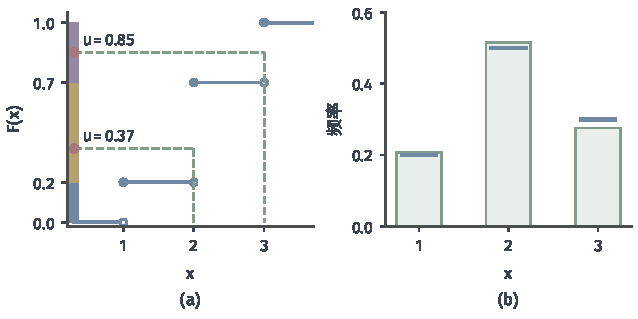
\includegraphics[width=108mm]{figures/07-probability/08-sampling-and-integration/matplotlib/sgen-discrete-inverse/figure.pdf}
  \caption{离散分布$p=(0.2,0.5,0.3)$的逆变换采样。(a)蓝线是分布函数，纵轴上的蓝、黄、紫三段是累计区间$(0,0.2]$、$(0.2,0.7]$、$(0.7,1]$；绿色虚线从$u=0.37$与$u=0.85$出发，分别落到$2$和$3$。(b)绿色柱是$1000$个样本（种子$11$）的频率$0.208,0.516,0.276$，蓝色短横线是真实概率。}
  \label{fig:sgen-discrete-inverse}
\end{BookInlineFigure}

式~\eqref{eq:sgen-discrete-inverse}的计算量在于找到$u$落在哪一段。从$k=1$起逐段比较，需要比较的次数是$X$对应的下标$k$，平均$\sum_kkp_k$次；例中为$0.2+1.0+0.9=2.1$次。若先把各值按概率从大到小排列，同一分布的平均次数降为$1\cdot0.5+2\cdot0.3+3\cdot0.2=1.7$次。$K$很大时，可以预先存好累计概率，用二分查找，每次约$\log_2K$次比较。

含原子的连续分布也由同一公式处理。分布函数在原子处的跳跃，对应$Q$的一段水平平台：长度等于原子概率的一段$u$全部被送到同一个点。第~\ref{chap:probability-spaces}章的等待时间在$0$处有概率$0.3$的原子，$u\le0.3$时输出$0$，就是这种情形。

\paragraph{需要数值反演的情形}
很多分布的$F$可以计算，$Q$却没有解析式。例如$\operatorname{Gamma}(2,1)$的分布函数是
\begin{equation}
  F(x)=1-(1+x)\mathrm{e}^{-x},\qquad x\ge0,
  \label{eq:sgen-gamma2-cdf}
\end{equation}
方程$F(x)=u$解不出初等的$x$。这时只能用数值方法近似求$Q(u)$。最稳妥的是二分法，它只用到$F$的单调性和式~\eqref{eq:sgen-quantile}的等价关系。

二分法的依据是：对任意点$m$，判断$F(m)\ge u$是否成立，就知道$Q(u)\le m$还是$Q(u)>m$。若已知$Q(u)$落在区间$(a,b]$中，取中点$m=(a+b)/2$做一次判断，就能把区间缩小一半，同时保持“$Q(u)$在区间内”这一事实。$k$轮后区间长度为$(b-a)/2^{k}$，输出中点，误差不超过区间长度的一半。

\needspace{6\baselineskip}
\paragraph{变量}
\begin{itemize}
  \item $u\in(0,1)$：基础随机数，整个过程中不变。
  \item $a<b$：当前区间的端点，始终满足$F(a)<u\le F(b)$，于是$Q(u)\in(a,b]$。
  \item $m$：当前区间的中点。
\end{itemize}

\paragraph{初始化}
取一个区间$(a,b]$，使$F(a)<u\le F(b)$。例中取$u=0.37$，$a=0$，$b=8$，因为
\[
  F(0)=0<0.37,\qquad F(8)=1-9\mathrm{e}^{-8}\approx0.9970\ge0.37 .
\]

\needspace{6\baselineskip}
\paragraph{每轮更新}
\begin{enumerate}
  \item \textbf{取中点。}令$m=(a+b)/2$，计算$F(m)$。例中第一轮$m=4$，由式~\eqref{eq:sgen-gamma2-cdf}，
  \[
    F(4)=1-5\mathrm{e}^{-4}\approx0.9084 .
  \]
  \item \textbf{缩小区间。}若$F(m)\ge u$，则$Q(u)\le m$，令$b\leftarrow m$；否则$Q(u)>m$，令$a\leftarrow m$。例中$0.9084\ge0.37$，区间变为$(0,4]$。

  以后各轮的中点、函数值和新区间依次为
  \[
    \begin{aligned}
      m&=2,& F(2)&\approx0.5940,& &(0,2];\\
      m&=1,& F(1)&\approx0.2642,& &(1,2];\\
      m&=1.5,& F(1.5)&\approx0.4422,& &(1,1.5];\\
      m&=1.25,& F(1.25)&\approx0.3554,& &(1.25,1.5].
    \end{aligned}
  \]
  \item \textbf{停止。}区间长度不超过预先给定的$2\delta$时停止，输出中点。例中取$\delta=0.125$，第五轮后长度为$0.25$，停止。
\end{enumerate}
最终输出$\widetilde{x}=1.375$。用更多轮次算出的真值是$Q(0.37)\approx1.2910$，误差约$0.084$，在$\delta=0.125$以内。图~\ref{fig:sgen-bisection-inverse}(a)画出了五个中点。

\paragraph{反演误差怎样改变输出分布}
数值反演输出的不是$Q(U)$，而是近似值$\widetilde{X}=\widetilde{Q}(U)$。它的分布已经不是$F$，问题是偏差多大。下面的引理把每个$u$上的反演误差转成分布函数的偏差。

\begin{lemma}[反演误差的传递]
\label{lem:sgen-inversion-error}
设$\delta\ge0$，函数$\widetilde{Q}$对一切$u\in(0,1)$满足$\lvert\widetilde{Q}(u)-Q(u)\rvert\le\delta$。记$\widetilde{F}$为$\widetilde{X}=\widetilde{Q}(U)$的分布函数，则对一切实数$x$，
\begin{equation}
  F(x-\delta)\le\widetilde{F}(x)\le F(x+\delta).
  \label{eq:sgen-inversion-band}
\end{equation}
若$F$还有不超过$L$的密度，则$\sup_x\lvert\widetilde{F}(x)-F(x)\rvert\le L\delta$。
\end{lemma}

\begin{proof}
若$\widetilde{X}\le x$，则$Q(U)\le\widetilde{X}+\delta\le x+\delta$，所以事件$\{\widetilde{X}\le x\}$包含于$\{Q(U)\le x+\delta\}$。取概率，由$Q(U)$的分布函数是$F$，得$\widetilde{F}(x)\le F(x+\delta)$。

反过来，若$Q(U)\le x-\delta$，则$\widetilde{X}\le Q(U)+\delta\le x$，所以$\{Q(U)\le x-\delta\}$包含于$\{\widetilde{X}\le x\}$，取概率得$F(x-\delta)\le\widetilde{F}(x)$。

若密度不超过$L$，则$F(x+\delta)-F(x)\le L\delta$，$F(x)-F(x-\delta)\le L\delta$，代入式~\eqref{eq:sgen-inversion-band}即得最后一句。
\end{proof}

引理的条件是“对所有$u$都有误差界$\delta$”，这一条在实际中容易被破坏。上面的二分法从固定区间$(0,8]$出发，当$u>F(8)\approx0.9970$时$Q(u)>8$，初始化条件不成立，二分法的每一轮都把区间推向右端，最终输出$7.875$，误差可以任意大。于是约$0.3\%$的尾部质量被搬到了$7.875$这一个点上。要保住误差界，初始化时须先把$b$向右扩大到$F(b)\ge u$为止。

即使误差界成立，输出的分布形状也可能改变。固定做五轮二分时，输出总是某个长$0.25$的小区间的中点，$\widetilde{X}$只取有限个值，是离散分布。图~\ref{fig:sgen-bisection-inverse}(b)画出它的分布函数：一条阶梯，夹在式~\eqref{eq:sgen-inversion-band}的两条紫色虚线之间。$\operatorname{Gamma}(2,1)$的密度$x\mathrm{e}^{-x}$的最大值是$\mathrm{e}^{-1}\approx0.368$，按引理，分布函数的偏差不超过$0.368\times0.125\approx0.046$；数值计算的最大偏差约为$0.0456$。用这样的样本估计依赖于细小尺度的量（例如落在某个短区间内的概率），偏差会比估计期望时明显。

\begin{BookInlineFigure}
  \centering
  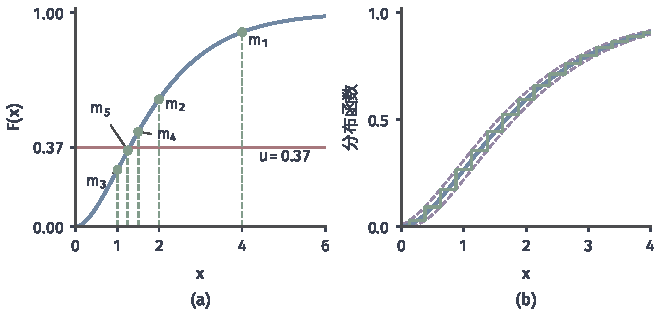
\includegraphics[width=112mm]{figures/07-probability/08-sampling-and-integration/matplotlib/sgen-bisection-inverse/figure.pdf}
  \caption{用二分法数值反演$\operatorname{Gamma}(2,1)$的分布函数。(a)蓝线是$F(x)=1-(1+x)\mathrm{e}^{-x}$，红线是$u=0.37$，绿点是五轮的中点$m_1,\dots,m_5=4,2,1,1.5,1.25$，最后区间为$(1.25,1.5]$。(b)固定做五轮时输出的分布函数（绿色阶梯）与$F$（蓝线），紫色虚线是$F(x-0.125)$与$F(x+0.125)$，阶梯始终夹在两者之间。}
  \label{fig:sgen-bisection-inverse}
\end{BookInlineFigure}

二分法每轮把误差减半，达到$\delta$需要约$\log_2((b-a)/\delta)$次分布函数求值。若$F$有可以计算的密度$f$，也可以用Newton迭代$x\leftarrow x-(F(x)-u)/f(x)$，在解附近每轮有效数字约翻一倍，但初值不好时可能越出定义域，常与二分法配合使用。不论用哪种方法，停止规则给出的误差界都要对全部$u$成立，引理~\ref{lem:sgen-inversion-error}才能用来估计输出分布的偏差。

\subsection{高斯样本生成}
\label{sec:sgen-gaussian}

高斯分布是最常用的目标，它的生成分两步：先生成独立的标准高斯坐标，再用一个仿射变换调出指定的均值与协方差。

\paragraph{独立标准高斯坐标}
标准高斯的分布函数$\Phi$连续且严格递增，由逆变换采样，$Z=\Phi^{-1}(U)$服从$\mathcal{N}(0,1)$。$\Phi^{-1}$没有初等表达式，常用的数值程序以有理函数逼近，在双精度下的误差已接近舍入误差，按引理~\ref{lem:sgen-inversion-error}，对输出分布的影响可以忽略。对$d$个相互独立的基础随机数分别作变换，
\[
  Z_j=\Phi^{-1}(U_j),\qquad j=1,\dots,d,
\]
各$Z_j$是不同基础随机数的函数，所以相互独立，组成的向量$\bm{Z}$服从$\mathcal{N}(\bm{0},\bm{I})$。式~\eqref{eq:sgen-box-muller}是另一种办法，每两个基础随机数给出两个独立的标准高斯数，只用到对数与三角函数。

例如取$u_1=0.37$、$u_2=0.80$，
\[
  z_1=\Phi^{-1}(0.37)\approx-0.3319,\qquad z_2=\Phi^{-1}(0.80)\approx0.8416 .
\]

\paragraph{仿射变换}
要生成$\mathcal{N}(\bm{\mu},\bm{\Sigma})$，其中$\bm{\mu}\in\mathbb{R}^{d}$是均值向量，$\bm{\Sigma}\in\mathbb{R}^{d\times d}$是对称半正定的协方差矩阵，先把$\bm{\Sigma}$分解为
\begin{equation}
  \bm{\Sigma}=\bm{A}\bm{A}^{\top},\qquad \bm{A}\in\mathbb{R}^{d\times r},
  \label{eq:sgen-cov-factor}
\end{equation}
再取$r$个独立标准高斯坐标组成$\bm{Z}$，令
\begin{equation}
  \bm{X}=\bm{\mu}+\bm{A}\bm{Z}.
  \label{eq:sgen-gaussian-affine}
\end{equation}
由期望的线性，$\mathbb{E}[\bm{X}]=\bm{\mu}$；由协方差在线性变换下的规则，
\[
  \operatorname{Cov}(\bm{X})=\bm{A}\operatorname{Cov}(\bm{Z})\bm{A}^{\top}=\bm{A}\bm{I}\bm{A}^{\top}=\bm{\Sigma}.
\]
第~\ref{chap:multivariate-distributions}章正是用这种形式定义多元高斯分布的，并证明了$\bm{\mu}+\bm{A}\bm{Z}$的分布只依赖于$\bm{A}\bm{A}^{\top}$，所以不论选哪个因子，都有$\bm{X}\sim\mathcal{N}(\bm{\mu},\bm{\Sigma})$。这一论证没有用到密度，因而不要求$\bm{\Sigma}$可逆。

因子$\bm{A}$有两种常用取法。$\bm{\Sigma}$正定时，Cholesky分解给出对角元为正的下三角矩阵$\bm{L}$，使$\bm{\Sigma}=\bm{L}\bm{L}^{\top}$，计算量约为$d^{3}/3$次乘法（可参考\BookChapterRef{chap:direct-linear-solvers}{卷二第12章“线性方程的直接求解”}）。$\bm{\Sigma}$只是半正定时，Cholesky分解会遇到零主元，可改用谱分解$\bm{\Sigma}=\bm{V}\bm{\Lambda}\bm{V}^{\top}$（可参考\BookChapterRef{chap:eigen-spectral-decomposition}{卷二第6章“谱分解”}），取$\bm{A}=\bm{V}\bm{\Lambda}^{1/2}$，并去掉特征值为零的列。分解只需做一次，之后每个样本只需$d$个标准高斯数和一次矩阵乘向量。

用一个二维例子走一遍。取
\[
  \bm{\mu}=\begin{bmatrix}1\\0\end{bmatrix},\qquad
  \bm{\Sigma}=\begin{bmatrix}4&2\\2&2\end{bmatrix},\qquad
  \bm{L}=\begin{bmatrix}2&0\\1&1\end{bmatrix},
\]
可以直接验证$\bm{L}\bm{L}^{\top}=\bm{\Sigma}$。代入上面的$z_1,z_2$，由式~\eqref{eq:sgen-gaussian-affine}，
\[
  \bm{x}=\begin{bmatrix}1+2z_1\\ z_1+z_2\end{bmatrix}\approx\begin{bmatrix}0.3363\\0.5098\end{bmatrix}.
\]
下三角结构使第一个坐标只用到$z_1$，第二个坐标用到$z_1$和$z_2$；两个坐标共用$z_1$，这正是它们的协方差$2$的来源。

\paragraph{奇异协方差}
若$\bm{\Sigma}$的秩$r<d$，式~\eqref{eq:sgen-gaussian-affine}仍然给出正确的分布，但$\bm{X}-\bm{\mu}=\bm{A}\bm{Z}$总落在$\bm{A}$的列空间中，这是一个$r$维子空间。例如
\[
  \bm{\Sigma}=\begin{bmatrix}1&2\\2&4\end{bmatrix}=\bm{a}\bm{a}^{\top},\qquad \bm{a}=\begin{bmatrix}1\\2\end{bmatrix},
\]
只需一个标准高斯数，$\bm{X}=\bm{\mu}+Z_1\bm{a}$全部落在过$\bm{\mu}$、方向为$\bm{a}$的直线上。这条直线在平面上的面积为零，$\bm{X}$在$\mathbb{R}^{2}$中没有密度，式~\eqref{eq:sgen-change-of-variables}无从使用；推前的论证不受影响。图~\ref{fig:sgen-gaussian-affine}对比了三种情形。

\begin{BookInlineFigure}
  \centering
  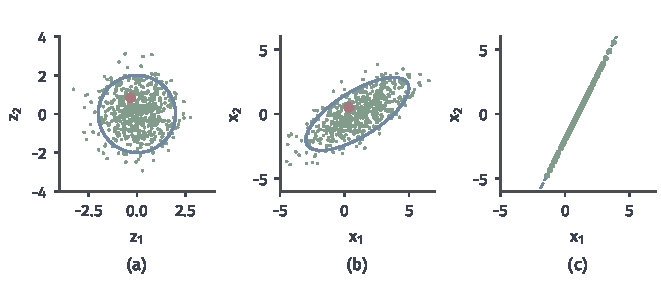
\includegraphics[width=112mm]{figures/07-probability/08-sampling-and-integration/matplotlib/sgen-gaussian-affine/figure.pdf}
  \caption{由独立标准高斯坐标生成指定协方差的高斯样本，$600$个样本（种子$5$）。(a)标准高斯$\bm{Z}$，蓝线是半径$2$的圆，红点是$(\Phi^{-1}(0.37),\Phi^{-1}(0.80))$；(b)$\bm{X}=\bm{\mu}+\bm{L}\bm{Z}$，$\bm{\mu}=(1,0)^{\top}$，$\bm{\Sigma}=\bm{L}\bm{L}^{\top}$，圆被变成椭圆，红点是例中的$(0.336,0.510)$；(c)秩为$1$的$\bm{\Sigma}=\bm{a}\bm{a}^{\top}$，样本全部落在蓝色虚线上。}
  \label{fig:sgen-gaussian-affine}
\end{BookInlineFigure}

奇异协方差在数值上还有一个隐患。若$\bm{\Sigma}$本应奇异，由于舍入它的最小特征值可能算成很小的负数，Cholesky分解随之失败；若$\bm{\Sigma}$本应正定但极接近奇异，分解得到的因子误差也会很大。谱分解可以把很小的负特征值截为零，但截断改变了协方差，偏差的大小应与$\bm{\Sigma}$的元素尺度一起报告。

\section{分步生成}
\label{sec:sgen-sequential}

有些目标分布找不到一个简单的整体映射，却可以拆成几个容易处理的部分。混合分布可以拆成“选哪一个成分”和“在成分内抽样”；多维分布可以按链式分解拆成“先抽第一个坐标，再按条件分布抽下一个坐标”。分步生成就是按这种拆分依次抽取，每一步只需要一个简单的生成方法。

检验分步生成是否正确，用的是全概率公式与链式分解：各步的分布按顺序拼起来，应当恰好拼回目标分布。拼接成立的前提是：每一步都取新的基础随机数，与前面各步用过的互不重叠。要注意这里的独立指的是输入：各步的基础随机数独立，并不意味着同一个样本的各个坐标独立，后一步的输出通常依赖前一步的输出。

\subsection{混合分布采样}
\label{sec:sgen-mixture}

设目标是有限混合
\begin{equation}
  \pi=\sum_{k=1}^{K}w_kP_k,\qquad w_k\ge0,\quad \sum_{k=1}^{K}w_k=1,
  \label{eq:sgen-mixture}
\end{equation}
其中每个成分$P_k$都能直接生成。全章的例子$0.3\,\mathcal{N}(-2,0.5^{2})+0.7\,\mathcal{N}(2,1)$就是这样：两个成分都是高斯分布，混合后却有两个峰，没有简单的分位数公式。

\paragraph{方法}
混合分布的意思是“先按权重选一个成分，再从这个成分中抽样”。按这个描述，用一个基础随机数$U_0$按累计权重$c_k=w_1+\dots+w_k$选出成分编号
\[
  J=k\quad\Longleftrightarrow\quad c_{k-1}<U_0\le c_k ,
\]
这正是式~\eqref{eq:sgen-discrete-inverse}；再用另一组基础随机数$\bm{U}'$生成$X=G_J(\bm{U}')$，其中$G_k$是第$k$个成分的生成方法。这种分步构造也称为\term{复合法}（composition method）。

\begin{theorem}[混合分布采样]
\label{thm:sgen-mixture}
设$U_0$与$\bm{U}'$独立，$\mathbb{P}(J=k)=w_k$，且对每个$k$，$G_k(\bm{U}')$的分布是$P_k$。则$X=G_J(\bm{U}')$的分布是式~\eqref{eq:sgen-mixture}中的$\pi$。
\end{theorem}

\begin{proof}
对任意事件$A$，按成分编号分解，
\[
  \mathbb{P}(X\in A)=\sum_{k=1}^{K}\mathbb{P}\bigl(J=k,\ G_k(\bm{U}')\in A\bigr).
\]
$J$只依赖$U_0$，$G_k(\bm{U}')$只依赖$\bm{U}'$，二者独立，所以每一项分解为乘积，
\[
  \mathbb{P}(X\in A)=\sum_{k=1}^{K}\mathbb{P}(J=k)\,\mathbb{P}\bigl(G_k(\bm{U}')\in A\bigr)=\sum_{k=1}^{K}w_kP_k(A)=\pi(A). \qedhere
\]
\end{proof}

这就是全概率公式：$J$把样本空间分成$K$块，每块内的条件分布是$P_k$。用例子走一遍：累计权重$c_1=0.3$、$c_2=1$，取$u_0=0.37>0.3$，选第二个成分；再取$u_1=0.80$，由逆变换得$\Phi^{-1}(0.80)\approx0.8416$，于是
\[
  x=2+1\times0.8416=2.8416 .
\]
生成一个样本用了两个基础随机数：一个选成分，一个在成分内生成。一般地，用量是$1$加上所选成分的用量，平均为$1+\sum_kw_k\,(\text{第}k\text{个成分的用量})$。

\paragraph{共用随机数会怎样}
定理~\ref{thm:sgen-mixture}的证明中，唯一用到的性质是$J$与$\bm{U}'$独立。若为了省一个随机数，让同一个$U$既选成分又在成分内生成，即$X=m_J+s_J\Phi^{-1}(U)$，结论就不再成立。$U\le0.3$时选第一个成分，但此时$\Phi^{-1}(U)\le\Phi^{-1}(0.3)$，只能得到第一个成分的下方$30\%$；$U>0.3$时只能得到第二个成分的上方$70\%$。计算可得，输出在$x\le-2+0.5\,\Phi^{-1}(0.3)\approx-2.262$上的密度是$\varphi((x+2)/0.5)/0.5$，在$x>2+\Phi^{-1}(0.3)\approx1.476$上的密度是$\varphi(x-2)$，中间没有质量。各成分的总权重仍然是$0.3$和$0.7$，形状却完全错了。图~\ref{fig:sgen-mixture}对比了两种做法。

\begin{BookInlineFigure}
  \centering
  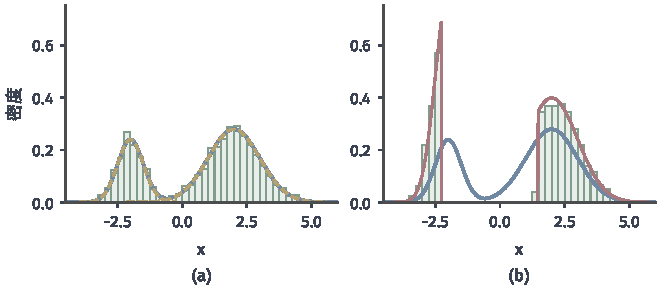
\includegraphics[width=112mm]{figures/07-probability/08-sampling-and-integration/matplotlib/sgen-mixture/figure.pdf}
  \caption{混合分布$0.3\,\mathcal{N}(-2,0.5^{2})+0.7\,\mathcal{N}(2,1)$的分步生成，$4000$个样本（种子$3$）。(a)选成分与成分内生成使用独立的基础随机数，绿色直方图与蓝色目标密度吻合，黄色虚线是两个加权成分；(b)同一个$U$同时用于两步，直方图只覆盖第一个成分的左侧与第二个成分的右侧，红线是按正文算出的输出密度。}
  \label{fig:sgen-mixture}
\end{BookInlineFigure}

共用随机数并非一定出错，关键在于共用的部分是否仍与$J$独立。令$V=(U-c_{J-1})/w_J$，即把$U$在所选区间内的位置重新拉伸到$(0,1)$。对每个$k$和$0\le v\le1$，
\[
  \mathbb{P}(J=k,\ V\le v)=\mathbb{P}\bigl(c_{k-1}<U\le c_{k-1}+w_kv\bigr)=w_kv=\mathbb{P}(J=k)\,v,
\]
所以$V$服从$\operatorname{Unif}(0,1)$且与$J$独立，可以代替$\bm{U}'$使用。代价是精度：$w_k$很小时，$V$只继承了$U$的少数几位有效数字，在有限精度下取值很稀疏。除非随机数生成确实是瓶颈，否则直接取新的基础随机数更简单。

\paragraph{连续混合}
混合的成分编号也可以是连续参数。若$\pi(A)=\int P_{\theta}(A)\,\nu(\mathrm{d}\theta)$，就先按$\nu$抽出$\theta$，再按$P_{\theta}$抽$X$，证明与定理~\ref{thm:sgen-mixture}相同，只是求和换成积分。第~\ref{chap:multivariate-distributions}章的正态尺度混合就是一例：先抽$W\sim\operatorname{Gamma}(\nu/2,\nu/2)$，再抽$X\sim\mathcal{N}(0,1/W)$，得到的$X$服从$t_{\nu}$。

\subsection{按条件分布生成坐标}
\label{sec:sgen-ancestral}

多维目标往往没有整体的生成映射，但它的联合分布可以按坐标依次分解。设$\bm{X}=(X_1,\dots,X_d)$的联合分布写成
\begin{equation}
  \pi(\mathrm{d}x_1,\dots,\mathrm{d}x_d)=P_1(\mathrm{d}x_1)\,K_2(x_1,\mathrm{d}x_2)\cdots K_d(x_{1:d-1},\mathrm{d}x_d),
  \label{eq:sgen-chain-decomposition}
\end{equation}
其中$P_1$是$X_1$的边缘分布，$K_j(x_{1:j-1},\cdot)$是给定前$j-1$个坐标时$X_j$的条件分布，$x_{1:j-1}$是$(x_1,\dots,x_{j-1})$的简写。第~\ref{chap:conditional-distributions}章证明了，在一般的取值空间上，这样的分解总是存在。生成时只要每个条件分布都能抽样。

\paragraph{方法与正确性}
先用$U_1$生成$X_1\sim P_1$；对$j=2,\dots,d$，用新的基础随机数$U_j$生成
\[
  X_j=G_j(X_{1:j-1},U_j),
\]
其中对每个固定的$x_{1:j-1}$，$G_j(x_{1:j-1},U_j)$的分布是$K_j(x_{1:j-1},\cdot)$。这种按顺序生成坐标的方法称为\term{祖先采样}（ancestral sampling）。

正确性按$j$归纳。设$(X_1,\dots,X_{j-1})$的分布已经是$\pi$的前$j-1$个坐标的边缘分布。$U_j$与$X_{1:j-1}$独立，因为后者只用了$U_1,\dots,U_{j-1}$；给定$X_{1:j-1}=x_{1:j-1}$时$X_j$的条件分布因而就是$G_j(x_{1:j-1},U_j)$的分布，即$K_j(x_{1:j-1},\cdot)$。由第~\ref{chap:conditional-distributions}章“边缘分布与概率核确定联合分布”的结论，$(X_1,\dots,X_j)$的分布是前一步的边缘分布与$K_j$的复合，也就是式~\eqref{eq:sgen-chain-decomposition}的前$j$个因子。$j=d$时得到$\pi$。

\paragraph{二元高斯的例子}
取标准化的二元高斯，相关系数$\rho=0.8$：
\[
  \bm{X}\sim\mathcal{N}\Biggl(\bm{0},\begin{bmatrix}1&\rho\\\rho&1\end{bmatrix}\Biggr).
\]
由第~\ref{chap:multivariate-distributions}章的高斯条件分布，给定$X_1=x_1$时$X_2\sim\mathcal{N}(\rho x_1,1-\rho^{2})$。于是祖先采样为
\begin{equation}
  X_1=\Phi^{-1}(U_1),\qquad X_2=\rho X_1+\sqrt{1-\rho^{2}}\,\Phi^{-1}(U_2).
  \label{eq:sgen-bivariate-ancestral}
\end{equation}
取$u_1=0.37$、$u_2=0.80$，$\sqrt{1-\rho^{2}}=0.6$，得到
\[
  x_1\approx-0.3319,\qquad x_2\approx0.8\times(-0.3319)+0.6\times0.8416\approx0.2395 .
\]
$U_1$与$U_2$独立，但$X_1$与$X_2$的相关系数是$0.8$：第二步把第一步的结果$X_1$作为输入用掉了。式~\eqref{eq:sgen-bivariate-ancestral}其实就是$\bm{\Sigma}$的Cholesky因子作用于$(\Phi^{-1}(U_1),\Phi^{-1}(U_2))$，与第~\ref{sec:sgen-gaussian}节的仿射方法一致。

\paragraph{两种“逐坐标”的区别}
祖先采样每生成一个完整的向量，都从第一个坐标重新开始，并使用一组新的基础随机数。第$i$个向量只用第$i$组随机数，所以各向量相互独立、同分布。另有一种做法看起来相似：手里保留一个完整的状态向量，每次只按“给定其余所有坐标”的条件分布重新抽一个坐标，其余坐标保持不变。这就是第~\ref{sec:sgen-gibbs}节的Gibbs采样。图~\ref{fig:sgen-sequential-scheme}画出两者的数据流。

\begin{BookInlineFigure}
  \centering
  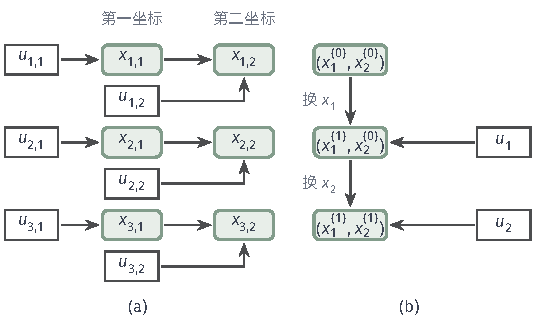
\includegraphics[width=91mm]{figures/07-probability/08-sampling-and-integration/tikz/sgen-sequential-scheme/figure.pdf}
  \caption{两种按坐标生成的数据流，方框是基础随机数，绿色圆角框是生成的坐标或状态。(a)祖先采样：每一行用自己的$u_{i,1},u_{i,2}$从头生成一个向量，行与行之间没有共用的输入；(b)Gibbs采样：保留状态，每次只换一个坐标，相邻状态共用未被更换的坐标。}
  \label{fig:sgen-sequential-scheme}
\end{BookInlineFigure}

两者用到的条件分布也不同。祖先采样需要的是按顺序的条件分布$K_j(x_{1:j-1},\cdot)$，只依赖排在前面的坐标；Gibbs采样需要的是给定其余全部坐标的条件分布。对二元高斯两者都容易得到，但在许多问题中只有后一种可以计算，这时只能退而使用链式更新。代价是：Gibbs采样的相邻状态共用坐标，因而相关，而且一般要从目标分布以外的状态出发。

\section{拒绝采样}
\label{sec:sgen-rejection}

前两节都要求目标分布有可以计算的分位数或可以抽样的分解。很多目标只给出一个密度公式，而且常常只知道到一个常数因子：$\pi(x)=\widetilde{p}(x)/Z$，其中$\widetilde{p}\ge0$可以逐点计算，归一化常数$Z=\int\widetilde{p}(x)\,\mathrm{d}x$却算不出来。模拟退火中的Gibbs分布$\exp(-f(x)/T)/Z_T$就是这样的目标（可参考\BookChapterRef{chap:random-search}{卷五第15章“随机搜索”}），状态多时$Z_T$是一个无法逐项求和的大和式。拒绝采样处理这类目标：从一个容易抽样的\term{建议分布}（proposal distribution）多抽一些候选，再按目标与建议的密度之比筛掉一部分。

这和用随机投点估计面积是同一个想法。在$\widetilde{p}$的图像下方均匀投点，点的横坐标就服从$\pi$；要在图像下方均匀投点，可以先在一个更大、容易投点的区域里均匀投点，再丢掉落在图像上方的点。

\subsection{接受规则的正确性}
\label{sec:sgen-rejection-correct}

设目标的未归一化密度$\widetilde{p}\ge0$满足$0<Z<\infty$；建议分布有密度$q$，可以直接抽样，密度可以计算；存在常数$M>0$，使
\begin{equation}
  \widetilde{p}(x)\le M\,q(x)\qquad\text{对一切}x\text{成立}.
  \label{eq:sgen-envelope}
\end{equation}
$Mq$称为包络，$M$称为\term{包络常数}（envelope constant）。式~\eqref{eq:sgen-envelope}蕴含：凡是$\widetilde{p}(x)>0$的地方都有$q(x)>0$，即建议分布覆盖了目标的全部质量所在。

\paragraph{一次试验}
抽候选$Y\sim q$，再抽与之独立的基础随机数$V$，当
\begin{equation}
  V\le\frac{\widetilde{p}(Y)}{M\,q(Y)}
  \label{eq:sgen-accept-rule}
\end{equation}
时接受$Y$，否则拒绝。$Y$落在$q(Y)=0$处的概率为零，比值总是有定义的；由式~\eqref{eq:sgen-envelope}，比值在$[0,1]$中，可以当作概率。几何上，点$(Y,\,V\,Mq(Y))$在包络$Mq$的图像下方均匀分布，接受规则就是“点落在$\widetilde{p}$的图像下方”。

\begin{theorem}[拒绝采样]
\label{thm:sgen-rejection}
在上述条件下，一次试验的接受概率是
\begin{equation}
  \mathbb{P}(\text{接受})=\frac{Z}{M},
  \label{eq:sgen-acceptance}
\end{equation}
给定接受时$Y$的条件分布是$\pi$。若独立重复试验直到第一次接受，记所用的试验次数为$N$、接受的候选为$X$，则$X\sim\pi$，$N\sim\operatorname{Geom}(Z/M)$，并且$X$与$N$独立。
\end{theorem}

\begin{proof}
对任意事件$A$，先对$Y$取条件，再对$Y$的密度积分。给定$Y=y$，接受的概率是$\widetilde{p}(y)/(Mq(y))$，因为$V$与$Y$独立。于是
\[
  \mathbb{P}(Y\in A,\ \text{接受})=\int_{A}q(y)\,\frac{\widetilde{p}(y)}{M\,q(y)}\,\mathrm{d}y=\frac{1}{M}\int_{A}\widetilde{p}(y)\,\mathrm{d}y=\frac{Z}{M}\,\pi(A).
\]
其中$q(y)=0$的点对积分没有贡献，由式~\eqref{eq:sgen-envelope}，那里$\widetilde{p}(y)=0$。取$A$为全空间，得到式~\eqref{eq:sgen-acceptance}。两式相除，$\mathbb{P}(Y\in A\mid\text{接受})=\pi(A)$。

记$a=Z/M$。各次试验使用互不重叠的基础随机数，相互独立。第$n$次才首次接受且接受的候选落在$A$中，意味着前$n-1$次都拒绝、第$n$次接受且候选在$A$中，所以
\[
  \mathbb{P}(N=n,\ X\in A)=(1-a)^{n-1}\cdot a\,\pi(A).
\]
对$A$取全空间得$\mathbb{P}(N=n)=(1-a)^{n-1}a$，即$N\sim\operatorname{Geom}(a)$；对$n$求和得$\mathbb{P}(X\in A)=\pi(A)$。联合概率等于两者之积，所以$X$与$N$独立。
\end{proof}

定理中各条件的作用如下。$0<Z<\infty$保证$\pi$是概率分布，也保证接受概率为正，否则会无限试下去。式~\eqref{eq:sgen-envelope}保证接受规则中的比值不超过$1$；它一旦失效，正确性随之失效，下面会看到后果。$V$与$Y$独立、各次试验独立，分别用在证明的第一步和第二步。整个算法只用到$\widetilde{p}$，不需要$Z$：$Z$的值只影响接受得多还是少，不影响接受下来的样本的分布。反过来，$M$必须真正满足式~\eqref{eq:sgen-envelope}，这是算法唯一需要预先保证的数。

\needspace{6\baselineskip}
\paragraph{变量}
\begin{itemize}
  \item $y$：当前候选，由建议分布生成。
  \item $v$：与候选配对的基础随机数，用于接受判定。
  \item $n$：已进行的试验次数。
\end{itemize}

\paragraph{初始化}
令$n=0$。下面用的例子是目标$\widetilde{p}(x)=x(1-x)$（$0\le x\le1$），建议分布$q=\operatorname{Unif}(0,1)$。$\widetilde{p}$在$x=1/2$处取最大值$1/4$，所以取$M=1/4$即满足式~\eqref{eq:sgen-envelope}。$Z=\int_0^1x(1-x)\,\mathrm{d}x=1/6$，归一化后$\pi(x)=6x(1-x)$是$\operatorname{Beta}(2,2)$的密度，但算法用不到这两个量。

\needspace{6\baselineskip}
\paragraph{每轮更新}
\begin{enumerate}
  \item \textbf{抽候选。}抽$y\sim q$与基础随机数$v$，令$n\leftarrow n+1$。例中第一轮用两个基础随机数$y=0.9$、$v=0.5$。
  \item \textbf{计算比值。}计算$r=\widetilde{p}(y)/(Mq(y))$。例中第一轮
  \[
    r=\frac{0.9\times0.1}{1/4}=0.36 .
  \]
  \item \textbf{判定。}若$v\le r$，接受$y$并停止；否则回到第1步。例中$0.5>0.36$，拒绝。第二轮取$y=0.37$、$v=0.80$，
  \[
    r=\frac{0.37\times0.63}{1/4}=0.9324\ge0.80,
  \]
  接受。
\end{enumerate}
最终得到样本$x=0.37$，用了$n=2$次试验、$4$个基础随机数。图~\ref{fig:sgen-rejection-envelope}(a)把这两次试验画成点$(y,\,vMq(y))$：$(0.9,0.125)$在抛物线上方，$(0.37,0.2)$在下方。

\begin{BookInlineFigure}
  \centering
  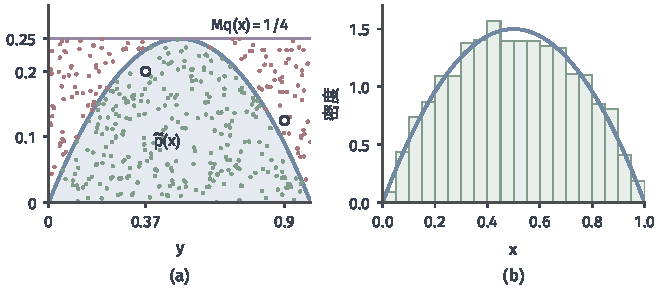
\includegraphics[width=112mm]{figures/07-probability/08-sampling-and-integration/matplotlib/sgen-rejection-envelope/figure.pdf}
  \caption{从$\operatorname{Unif}(0,1)$拒绝采样$\operatorname{Beta}(2,2)$，$\widetilde{p}(x)=x(1-x)$，$M=1/4$。(a)$400$个候选画成点$(y,\,vMq(y))$（种子$2$），紫线是包络$Mq=1/4$，蓝线下方浅蓝区域里的绿点被接受，上方的红点被拒绝；两个空心圆是正文中的两次试验。(b)$6000$个候选中被接受的点的直方图（接受比例$0.6625$），蓝线是$6x(1-x)$。}
  \label{fig:sgen-rejection-envelope}
\end{BookInlineFigure}

\paragraph{包络无效时}
若式~\eqref{eq:sgen-envelope}在某些点不成立，比值$\widetilde{p}/(Mq)$在那里超过$1$，判定$v\le r$必然通过，实际的接受概率是$\min\{1,\widetilde{p}/(Mq)\}$。把定理的第一步计算中的$\widetilde{p}/(Mq)$换成这个量，接受样本的密度正比于
\begin{equation}
  q(x)\min\Bigl\{1,\frac{\widetilde{p}(x)}{M\,q(x)}\Bigr\}=\frac{1}{M}\min\bigl\{\widetilde{p}(x),\,M\,q(x)\bigr\}.
  \label{eq:sgen-invalid-envelope}
\end{equation}
也就是说，目标在包络以上的部分被削平了。在上面的例子中错用$M=1/5$，$x(1-x)>1/5$的区间是$(0.276,0.724)$，输出的密度在这一段变成常数，中部的质量被系统地压低（图~\ref{fig:sgen-rejection-invalid}）。从直方图上看，偏差并不刺眼；程序也不会报错，因为每一步都“正常地”接受或拒绝。所以包络常数必须由推导保证，不能凭几次试算的最大比值来定。

\begin{BookInlineFigure}
  \centering
  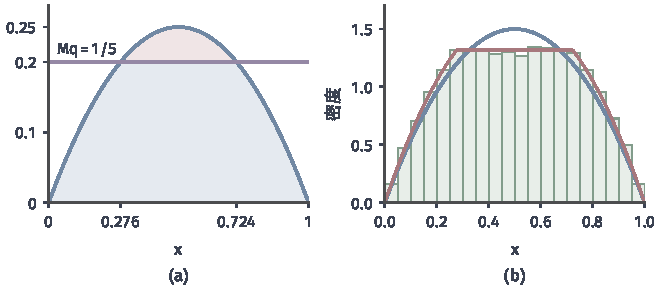
\includegraphics[width=112mm]{figures/07-probability/08-sampling-and-integration/matplotlib/sgen-rejection-invalid/figure.pdf}
  \caption{包络常数过小的后果。(a)蓝线是$\widetilde{p}(x)=x(1-x)$，紫线是错用的$Mq=1/5$，浅红区域是被削去的部分；(b)$20000$个候选中被接受点的直方图（种子$4$），红线是按式~\eqref{eq:sgen-invalid-envelope}归一化的输出密度，蓝线是目标$6x(1-x)$。}
  \label{fig:sgen-rejection-invalid}
\end{BookInlineFigure}

\subsection{接受率与生成成本}
\label{sec:sgen-rejection-cost}

拒绝采样总是正确的，问题在于要试多少次。由定理~\ref{thm:sgen-rejection}，试验次数$N$服从参数为$a=Z/M$的几何分布，于是得到一个样本平均所需的建议次数为
\begin{equation}
  \mathbb{E}[N]=\frac{M}{Z}.
  \label{eq:sgen-expected-trials}
\end{equation}
它就是包络下的面积$M$与目标下的面积$Z$之比，即投点区域中“浪费”的比例的倒数。例中$M/Z=(1/4)/(1/6)=1.5$，平均每个样本要试$1.5$次；图~\ref{fig:sgen-rejection-envelope}(b)中$6000$个候选的接受比例$0.6625$与理论值$2/3$相符。

若$\widetilde{p}=\pi$已经归一化，式~\eqref{eq:sgen-envelope}两边积分得$1\le M$，所以接受率$1/M$不超过$1$，等号当且仅当$q=\pi$（除去零概率集）。包络越贴近目标，$M$越接近$1$。

\paragraph{成本的组成}
一次试验的成本包括生成候选、计算$\widetilde{p}(y)$与$q(y)$、生成$v$。设一次试验的平均成本为$c$，得到$n$个样本的期望成本为$n\,c\,M/Z$，此外还有一次性的准备成本：求出有效的$M$。$M$最好取$\sup_x\widetilde{p}(x)/q(x)$，这需要解一个优化问题；取得太大虽然仍然正确，但成本按比例上升。两种成本的权衡在于：准备工作做一次，试验成本乘以样本数。

试验次数的波动也要计入。$N$的方差是$(1-a)/a^{2}$，接受率低时次数的分布有很长的右尾，生成固定个数的样本所需时间也随之波动。

\paragraph{高维中的接受率}
包络在高维中很难贴紧。设目标是$\mathcal{N}(\bm{0},\bm{I}_d)$，建议分布是$\mathcal{N}(\bm{0},\sigma^{2}\bm{I}_d)$，$\sigma>1$。两个归一化密度之比为
\[
  \frac{\pi(\bm{x})}{q(\bm{x})}=\sigma^{d}\exp\Bigl(-\frac{\lVert\bm{x}\rVert_2^{2}}{2}\bigl(1-\sigma^{-2}\bigr)\Bigr)\le\sigma^{d},
\]
等号在$\bm{x}=\bm{0}$处成立，所以最小的包络常数是$M=\sigma^{d}$，接受率为
\begin{equation}
  a=\sigma^{-d}.
  \label{eq:sgen-acceptance-dimension}
\end{equation}
每个坐标上建议分布只比目标宽一点，接受率也随维数指数下降。$\sigma=1.1$时，$d=10$的接受率约为$0.386$，$d=100$时约为$7.3\times10^{-5}$，平均每个样本要试一万多次。若$\sigma<1$，比值在$\lVert\bm{x}\rVert_2\to\infty$时趋于无穷，根本不存在包络：建议分布的尾部必须不比目标轻。

\begin{BookInlineFigure}
  \centering
  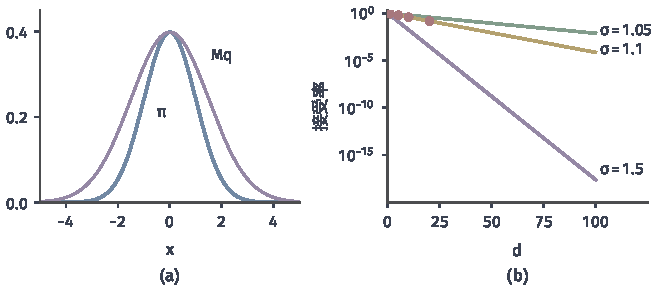
\includegraphics[width=112mm]{figures/07-probability/08-sampling-and-integration/matplotlib/sgen-rejection-dimension/figure.pdf}
  \caption{高斯目标、高斯建议时的拒绝采样。(a)$d=1$、$\sigma=1.5$，蓝线是目标$\pi$，紫线是包络$Mq$，二者只在$x=0$处相切；(b)接受率$\sigma^{-d}$随维数$d$的变化（对数纵轴），绿、黄、紫依次为$\sigma=1.05,1.1,1.5$，红点是$\sigma=1.1$、$d=1,5,10,20$时各$20$万个候选的模拟接受比例（种子$8$）。}
  \label{fig:sgen-rejection-dimension}
\end{BookInlineFigure}

图~\ref{fig:sgen-rejection-dimension}(a)说明了原因：包络只在一点与目标相切，其余地方都留有空隙，空隙所占的比例按维数相乘。一维时浪费不到一半，一百维时几乎全部浪费。拒绝采样在低维、能找到贴身包络的问题中很有效，在高维中通常只作为其他方法的一个组成部分。对那些连有效包络都写不出来的高维目标，需要换一种思路，这就是下一节的链式更新。

\section{MCMC采样}
\label{sec:sgen-mcmc}

直接生成要求一次性造出一个完整的目标样本，这需要分位数、可抽样的分解或贴身的包络。高维目标往往三者都没有，能做的只是逐点计算未归一化密度$\widetilde{p}(x)$，或者计算它的梯度。只靠这些局部信息，能否得到目标分布的样本？

\term{Markov链Monte Carlo}（Markov chain Monte Carlo，MCMC）的回答是：不再从头造样本，而是让一个状态在空间中游走，每一步只根据当前位置随机地走到下一个位置，并设计走法，使目标概率大的地方被访问得更频繁。把目标分布想象成地形的高度，游走者在高处停留得久、在低处停留得短，长时间下来，在各处停留的时间比例就接近目标概率。这个图景有两处需要准确化：“走法不破坏目标分布”是一个可以逐步验证的代数条件，即下面的不变性；“长时间后停留比例接近目标”则还需要链能走遍目标的支持，这是另一个条件，不能由第一个推出。

本节先建立转移与不变分布，再介绍保持目标不变的三种更新，它们分别以Metropolis--Hastings、Gibbs和Hamilton命名。它们的输出都是一串相关的状态，而不是独立样本。

\subsection{转移与不变分布}
\label{sec:sgen-invariance}

\paragraph{转移核}
链式更新的每一步，都是在给定当前状态$x$时，随机地选出下一个状态。把“给定$x$时下一状态的分布”记作$K(x,\cdot)$：对状态空间中的集合$A$，$K(x,A)$是从$x$出发一步后进入$A$的概率。按第~\ref{chap:conditional-distributions}章的定义，$K$是从状态空间到自身的概率核，在这里称为\term{转移核}（transition kernel）。状态有限时，$K$就是一个每行和为$1$的非负矩阵，第$x$行第$y$列为$K(x,\{y\})$。

用转移核生成一条链：给定初始状态$X^{(0)}$，对$t=0,1,2,\dots$，用新的基础随机数从$K(X^{(t)},\cdot)$中抽出$X^{(t+1)}$。具体实现中，常写成$X^{(t+1)}=\Psi(X^{(t)},\bm{U}^{(t+1)})$，其中$\Psi$是确定的更新函数，$\bm{U}^{(t+1)}$是第$t+1$步专用的基础随机数，并且对每个$x$，$\Psi(x,\bm{U})$的分布是$K(x,\cdot)$。由于各步的随机数互不重叠，给定$X^{(t)}$后，$X^{(t+1)}$与更早的状态无关，这正是Markov链的含义，第~\ref{chap:information-measures}章对三个变量用过的Markov性在这里对整个序列成立。

\paragraph{分布的传播}
若$X^{(t)}$的分布是$\mu_t$，下一步的分布是多少？$\bm{U}^{(t+1)}$与$X^{(t)}$独立，给定$X^{(t)}=x$时$X^{(t+1)}$的条件分布是$K(x,\cdot)$。由第~\ref{chap:conditional-distributions}章边缘分布与概率核复合的公式，
\begin{equation}
  \mu_{t+1}(A)=\int K(x,A)\,\mu_t(\mathrm{d}x),\qquad\text{记作}\quad\mu_{t+1}=\mu_tK .
  \label{eq:sgen-distribution-step}
\end{equation}
状态有限时，这就是行向量乘矩阵：$\mu_{t+1}=\mu_t\bm{K}$。

\paragraph{不变分布}
如果某个分布在一步更新后不变，从它出发就永远保持在它上面。

\begin{definition}[不变分布]
\label{def:sgen-invariant}
若状态空间上的概率分布$\pi$对一切可测集$A$满足
\begin{equation}
  \int K(x,A)\,\pi(\mathrm{d}x)=\pi(A),
  \label{eq:sgen-invariance}
\end{equation}
即$\pi K=\pi$，则称$\pi$是转移核$K$的\term{不变分布}（invariant distribution），也称平稳分布。
\end{definition}

若$X^{(0)}\sim\pi$且$\pi$是不变分布，由式~\eqref{eq:sgen-distribution-step}按$t$归纳，每个$X^{(t)}$的边缘分布都是$\pi$。这时链的每一个状态单独看都是目标分布的样本，只是相邻状态之间一般不独立。MCMC构造的第一个要求，就是让目标分布$\pi$成为转移核的不变分布。

用一个三状态的例子检验定义。取状态$\{1,2,3\}$上的转移矩阵
\[
  \bm{K}=\begin{bmatrix}0.5&0.5&0\\0.2&0.5&0.3\\0&0.5&0.5\end{bmatrix},\qquad \pi=(0.2,0.5,0.3).
\]
逐列计算$\pi\bm{K}$：
\[
  \begin{aligned}
    (\pi\bm{K})_1&=0.2\times0.5+0.5\times0.2=0.2,\\
    (\pi\bm{K})_2&=0.2\times0.5+0.5\times0.5+0.3\times0.5=0.5,\\
    (\pi\bm{K})_3&=0.5\times0.3+0.3\times0.5=0.3,
  \end{aligned}
\]
所以$\pi$是不变分布。若从状态$1$出发，$\mu_0=(1,0,0)$，按式~\eqref{eq:sgen-distribution-step}逐步计算，
\[
  \mu_1=(0.5,0.5,0),\qquad \mu_2=(0.35,0.5,0.15),\qquad \mu_3=(0.275,0.5,0.225),
\]
各分量一步步向$\pi$靠拢。图~\ref{fig:sgen-chain-evolution}(a)画出了前几步，(b)是沿一条模拟路径计算的“停在状态$3$的时间比例”，它在约$2000$步后接近$0.3$。

\begin{BookInlineFigure}
  \centering
  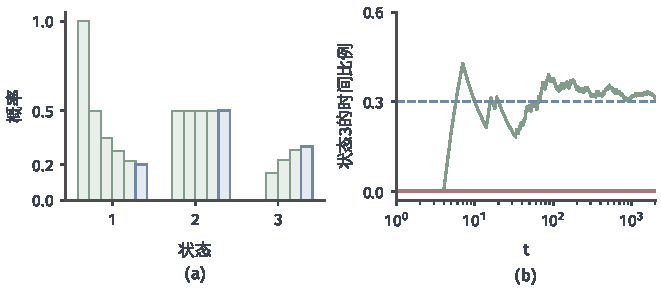
\includegraphics[width=112mm]{figures/07-probability/08-sampling-and-integration/matplotlib/sgen-chain-evolution/figure.pdf}
  \caption{三状态转移矩阵$\bm{K}$的分布传播与时间平均。(a)从状态$1$出发，每组左起五根绿色柱依次是$t=0,1,2,3,5$时的$\mu_t$，最右的蓝色柱是不变分布$\pi=(0.2,0.5,0.3)$；(b)一条模拟路径（种子$6$，横轴为对数刻度）上停在状态$3$的时间比例，绿线是$\bm{K}$，红线是“永远停在原地”的转移，蓝色虚线是$\pi(\{3\})=0.3$。}
  \label{fig:sgen-chain-evolution}
\end{BookInlineFigure}

\paragraph{不变不等于能到达}
不变性只说“从目标出发会留在目标”，不说“从别处出发会走到目标”。最极端的例子是始终停在原地的转移$K(x,\cdot)=\delta_x$，即单位矩阵。对它而言，任何分布都满足式~\eqref{eq:sgen-invariance}，目标分布当然也是不变分布。但从状态$1$出发，链永远停在$1$，停在状态$3$的时间比例恒为$0$，与$\pi(\{3\})=0.3$毫无关系，这就是图~\ref{fig:sgen-chain-evolution}(b)中的红线。

不那么极端的失败也很常见。若转移矩阵是分块对角的，例如状态$\{1,2\}$与$\{3\}$之间互不往来，从块$\{1,2\}$出发就永远看不到状态$3$。若转移在两个状态之间交替，$\bm{K}=\begin{bmatrix}0&1\\1&0\end{bmatrix}$，那么$(1/2,1/2)$是不变分布，从状态$1$出发的分布却在$(1,0)$与$(0,1)$之间来回摆动，永远不收敛，尽管时间比例趋于$1/2$。

所以MCMC的正确性分成两层。第一层是不变性，它是转移核的一个代数性质，下面三种更新都给出完整证明。第二层是从任意初值出发，分布收敛到$\pi$、时间平均收敛到目标期望，这需要状态之间能够互相到达（不可约）、链不陷入周期摆动（非周期）等条件。有限状态时，在不可约与非周期之下这两个结论都成立；一般状态空间需要更细的条件。这些长期性质的条件与证明可参考\BookChapterRef{chap:discrete-time-stochastic-processes}{卷九第3章“离散时间随机过程”}，也可查阅~\scite{math-meyn2009markov}。本章只证明不变性，并对每种更新指出它可能在哪里不能走遍目标。

\subsection{Metropolis--Hastings采样}
\label{sec:sgen-mh}

怎样构造一个以给定$\pi=\widetilde{p}/Z$为不变分布的转移？手里通常有一个容易抽样的局部建议，例如“在当前点附近随机迈一步”。这个建议本身一般不保持$\pi$，Metropolis--Hastings的做法是在建议之后加一道接受判定，把它修正成保持$\pi$的转移\scite{pgm-history-metropolis1953}\scite{pgm-history-hastings1970}。

\paragraph{主要思想：平衡每一对方向的概率流}
把$\pi$想象成状态之间的质量分配，转移一步就是把每个状态上的质量按转移概率分给各个状态。从$x$流向$y$的质量是$\pi(x)K(x,y)$，称为概率流。若每一对状态之间两个方向的流量相等，
\begin{equation}
  \pi(x)K(x,y)=\pi(y)K(y,x),
  \label{eq:sgen-detailed-balance-discrete}
\end{equation}
那么每个状态流出多少就流入多少，分布保持不变。这个条件称为\term{细致平衡}（detailed balance）。一般状态空间上，细致平衡写成对一切可测集$A,B$，
\begin{equation}
  \int_{A}K(x,B)\,\pi(\mathrm{d}x)=\int_{B}K(y,A)\,\pi(\mathrm{d}y),
  \label{eq:sgen-detailed-balance}
\end{equation}
即“从$A$流进$B$”等于“从$B$流进$A$”。

\begin{lemma}[细致平衡蕴含不变性]
\label{lem:sgen-detailed-balance}
若$\pi$与$K$满足式~\eqref{eq:sgen-detailed-balance}，则$\pi$是$K$的不变分布。
\end{lemma}

\begin{proof}
在式~\eqref{eq:sgen-detailed-balance}中取$A$为整个状态空间。左边是$\int K(x,B)\,\pi(\mathrm{d}x)$；右边中$K(y,\cdot)$是概率分布，$K(y,A)=1$，所以右边等于$\pi(B)$。这正是式~\eqref{eq:sgen-invariance}。
\end{proof}

细致平衡是充分条件而不是必要条件：沿圆周单向转圈的转移保持均匀分布不变，却在每一对方向上只有单向流量。它的好处是只需逐对检查，不必求和或积分，所以是构造转移最方便的工具。

现在设建议在状态$x$处的密度为$q(y\mid x)$（离散时是概率，连续时是关于Lebesgue测度的密度）。只用建议时，从$x$到$y$的流量正比于$\widetilde{p}(x)q(y\mid x)$，反向流量正比于$\widetilde{p}(y)q(x\mid y)$，二者一般不等。办法是把较大的一边按比例削减到较小的一边：从$x$到$y$的建议以概率$a(x,y)$接受，使
\[
  \widetilde{p}(x)q(y\mid x)a(x,y)=\min\bigl\{\widetilde{p}(x)q(y\mid x),\ \widetilde{p}(y)q(x\mid y)\bigr\}.
\]
右边关于$x,y$对称，流量自然平衡。解出$a$，得到
\begin{equation}
  a(x,y)=\min\Bigl\{1,\ \frac{\widetilde{p}(y)\,q(x\mid y)}{\widetilde{p}(x)\,q(y\mid x)}\Bigr\}.
  \label{eq:sgen-mh-acceptance}
\end{equation}
较小的一边接受概率为$1$，较大的一边按比值削减；被拒绝时留在原地。比值中$\widetilde{p}$出现在分子和分母，归一化常数$Z$约掉了，算法从头到尾不需要$Z$。

比值的定义需要交代。设当前状态$x$满足$\widetilde{p}(x)>0$，候选$y$由$q(\cdot\mid x)$产生，于是$q(y\mid x)>0$（概率为一），分母为正。若$\widetilde{p}(y)=0$或$q(x\mid y)=0$，比值为$0$，候选必被拒绝，所以链从$\{\widetilde{p}>0\}$出发就永远留在其中。

\begin{definition}[Metropolis--Hastings转移]
\label{def:sgen-mh}
设$\widetilde{p}\ge0$，$0<Z<\infty$，$S=\{x:\widetilde{p}(x)>0\}$。对$x\in S$，从$q(\cdot\mid x)$抽候选$y$，以式~\eqref{eq:sgen-mh-acceptance}的概率$a(x,y)$接受（令$X^{(t+1)}=y$），否则令$X^{(t+1)}=x$。对应的转移核为
\begin{equation}
  K(x,B)=\int_{B}q(y\mid x)\,a(x,y)\,\lambda(\mathrm{d}y)+r(x)\,\mathbf{1}_{B}(x),
  \label{eq:sgen-mh-kernel}
\end{equation}
其中$\lambda$是参考测度（计数测度或Lebesgue测度），
\begin{equation}
  r(x)=1-\int q(y\mid x)\,a(x,y)\,\lambda(\mathrm{d}y)
  \label{eq:sgen-mh-reject}
\end{equation}
是被拒绝而留在原地的概率。这种转移称为\term{Metropolis--Hastings算法}（Metropolis--Hastings algorithm）。
\end{definition}

\begin{theorem}[Metropolis--Hastings转移保持目标]
\label{thm:sgen-mh}
在定义~\ref{def:sgen-mh}的条件下，$\pi=\widetilde{p}/Z$与$K$满足细致平衡，因而$\pi$是$K$的不变分布。
\end{theorem}

\begin{proof}
对$\lambda$下的密度$\pi(x)=\widetilde{p}(x)/Z$，令
\[
  m(x,y)=\pi(x)\,q(y\mid x)\,a(x,y).
\]
先证
\[
  m(x,y)=\frac1Z\min\bigl\{\widetilde{p}(x)q(y\mid x),\ \widetilde{p}(y)q(x\mid y)\bigr\}.
\]
若$\widetilde{p}(x)q(y\mid x)>0$，把式~\eqref{eq:sgen-mh-acceptance}代入，乘开即得。若$\widetilde{p}(x)q(y\mid x)=0$，左边为零，右边的最小值也为零。所以$m(x,y)=m(y,x)$。

对可测集$A,B$，由式~\eqref{eq:sgen-mh-kernel}，
\[
  \int_{A}K(x,B)\,\pi(\mathrm{d}x)=\int_{A}\int_{B}m(x,y)\,\lambda(\mathrm{d}y)\,\lambda(\mathrm{d}x)+\int_{A\cap B}r(x)\,\pi(\mathrm{d}x).
\]
被积函数非负，可以交换积分次序；再用$m$的对称性，第一项对$A$与$B$对称。第二项是$r\pi$在$A\cap B$上的积分，本身对$A$与$B$对称。于是式~\eqref{eq:sgen-detailed-balance}成立，由引理~\ref{lem:sgen-detailed-balance}，$\pi$是不变分布。
\end{proof}

证明只用到两件事：接受概率使双向流量对称，被拒绝的质量留在原地。建议分布可以是任何能抽样、能计算密度的分布，这是Metropolis--Hastings的灵活之处。

\paragraph{为什么需要建议比}
若建议对称，$q(y\mid x)=q(x\mid y)$，式~\eqref{eq:sgen-mh-acceptance}简化为$\min\{1,\widetilde{p}(y)/\widetilde{p}(x)\}$，称为\term{Metropolis算法}（Metropolis algorithm）。模拟退火中的接受规则$\min\{1,\exp(-(f(y)-f(x))/T)\}$就是取$\widetilde{p}=\exp(-f/T)$的Metropolis规则。建议不对称时若仍用这个简化的比值，不变分布就会偏离目标，下面的三状态例子会算出偏离的结果。$q(x\mid y)/q(y\mid x)$这一项就是对建议偏向的修正：建议更爱往$y$走，就相应减少往$y$走的接受。

\paragraph{计算过程}
用$\{1,2,3\}$上的目标$\widetilde{p}=(2,5,3)$演示，$Z=10$对算法未知，$\pi=(0.2,0.5,0.3)$。建议在一条链上移动：从$1$总是建议$2$，从$3$总是建议$2$，从$2$以各$1/2$的概率建议$1$或$3$。建议不对称，例如$q(2\mid1)=1$而$q(1\mid2)=1/2$。

\needspace{6\baselineskip}
\paragraph{变量}
\begin{itemize}
  \item $x$：当前状态；$y$：候选状态。
  \item $a$：本步的接受概率，由式~\eqref{eq:sgen-mh-acceptance}计算。
  \item $u_{\mathrm{q}}$、$u_{\mathrm{a}}$：每步的两个基础随机数，前者用于抽候选（只在状态$2$需要），后者用于接受判定。
\end{itemize}

\paragraph{初始化}
取$x^{(0)}\in S$。例中$x^{(0)}=1$。四种可能的移动对应的接受概率可以预先算好：
\[
  \begin{aligned}
    a(1,2)&=\min\Bigl\{1,\frac{5\times\frac12}{2\times1}\Bigr\}=1,&\qquad
    a(2,1)&=\min\Bigl\{1,\frac{2\times1}{5\times\frac12}\Bigr\}=0.8,\\
    a(2,3)&=\min\Bigl\{1,\frac{3\times1}{5\times\frac12}\Bigr\}=1,&\qquad
    a(3,2)&=\min\Bigl\{1,\frac{5\times\frac12}{3\times1}\Bigr\}=\frac56.
  \end{aligned}
\]

\needspace{6\baselineskip}
\paragraph{每轮更新}
在第$t+1$步：
\begin{enumerate}
  \item \textbf{抽候选。}从$q(\cdot\mid x^{(t)})$抽$y$。例中状态$2$处，$u_{\mathrm{q}}\le0.5$时建议$1$，否则建议$3$；第一步$x^{(0)}=1$，候选$y=2$。

  \item \textbf{计算接受概率。}按式~\eqref{eq:sgen-mh-acceptance}计算$a(x^{(t)},y)$。例中第一步$a(1,2)=1$。

  \item \textbf{判定。}若$u_{\mathrm{a}}\le a$，令$x^{(t+1)}=y$；否则$x^{(t+1)}=x^{(t)}$。例中第一步$u_{\mathrm{a}}=0.37\le1$，接受，$x^{(1)}=2$。

  后四步使用的随机数与结果如下（空格表示该步不需要$u_{\mathrm{q}}$）：
  \begin{center}
    \small
    \begin{tabular}{@{}ccccccc@{}}
      \toprule
      $t$ & $x^{(t-1)}$ & $u_{\mathrm{q}}$ & $y$ & $a$ & $u_{\mathrm{a}}$ & $x^{(t)}$\\
      \midrule
      $2$ & $2$ & $0.62$ & $3$ & $1$ & $0.90$ & $3$（接受）\\
      $3$ & $3$ & & $2$ & $5/6$ & $0.88$ & $3$（拒绝）\\
      $4$ & $3$ & & $2$ & $5/6$ & $0.41$ & $2$（接受）\\
      $5$ & $2$ & $0.20$ & $1$ & $0.8$ & $0.85$ & $2$（拒绝）\\
      \bottomrule
    \end{tabular}
  \end{center}

  \item \textbf{停止。}做满预定的步数后停止。链本身没有自然的终点，步数要按下一章的误差分析决定。
\end{enumerate}
最终得到状态序列$1,2,3,3,2,2$。被拒绝的两步都把当前状态重复记录了一次，这些重复是转移的一部分，必须保留：删掉它们，状态$3$与状态$2$被访问的频率就会改变。

把接受概率乘上建议概率，得到转移矩阵
\[
  \bm{K}=\begin{bmatrix}0&1&0\\0.4&0.1&0.5\\0&\frac56&\frac16\end{bmatrix},
\]
其中$K(2,2)=1-0.4-0.5=0.1$与$K(3,3)=1/6$来自拒绝。逐对验证细致平衡：
\[
  \pi(1)K(1,2)=0.2=\pi(2)K(2,1),\qquad \pi(2)K(2,3)=0.25=\pi(3)K(3,2).
\]
图~\ref{fig:sgen-mh-three-state}画出建议与修正后的转移。

\begin{BookInlineFigure}
  \centering
  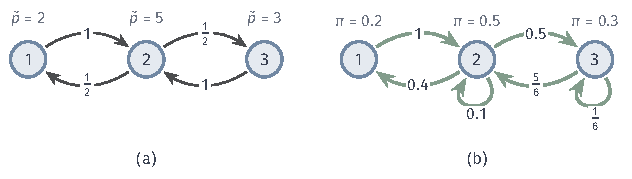
\includegraphics[width=107mm]{figures/07-probability/08-sampling-and-integration/tikz/sgen-mh-three-state/figure.pdf}
  \caption{三状态目标$\widetilde{p}=(2,5,3)$上的Metropolis--Hastings。(a)建议$q$：从端点总是走向中间，从中间各以$1/2$走向两端；(b)修正后的转移核，绿色箭头上是转移概率，自环来自拒绝。两个方向的概率流相等：$1\leftrightarrow2$都是$0.2$，$2\leftrightarrow3$都是$0.25$。}
  \label{fig:sgen-mh-three-state}
\end{BookInlineFigure}

若省去建议比，只用$\min\{1,\widetilde{p}(y)/\widetilde{p}(x)\}$，则$a(2,1)=0.4$、$a(2,3)=0.6$、$a(1,2)=a(3,2)=1$，转移矩阵的第二行变为$(0.2,0.5,0.3)$，第一、三行都是$(0,1,0)$。解$\pi\bm{K}=\pi$，由第一列得$\pi(1)=0.2\pi(2)$，由第三列得$\pi(3)=0.3\pi(2)$，归一化后
\[
  \pi=\Bigl(\frac{2}{15},\ \frac{2}{3},\ \frac{1}{5}\Bigr)\ne(0.2,\ 0.5,\ 0.3).
\]
中间状态被建议得多，又没有被修正，于是被过度访问。

\paragraph{随机游走建议}
连续状态最常用的建议是在当前点加一个对称扰动，$y=x+s\,\varepsilon$，$\varepsilon\sim\mathcal{N}(0,1)$，称为\term{随机游走Metropolis算法}（random-walk Metropolis algorithm）。步长$s$决定了接受率与移动距离之间的取舍。图~\ref{fig:sgen-rwmh-traces}在全章的混合目标上从$x=-2$出发各运行$3000$步：$s=0.3$时接受率约$0.83$，每步移动很小，链在左峰停留了很久，只有约$8\%$的时间在右边（目标是$70\%$）；$s=30$时几乎每个候选都落在目标概率很小的远处，接受率约$0.064$，链大段时间原地不动；$s=2.5$时接受率约$0.47$，两峰之间往来频繁。

\begin{BookInlineFigure}
  \centering
  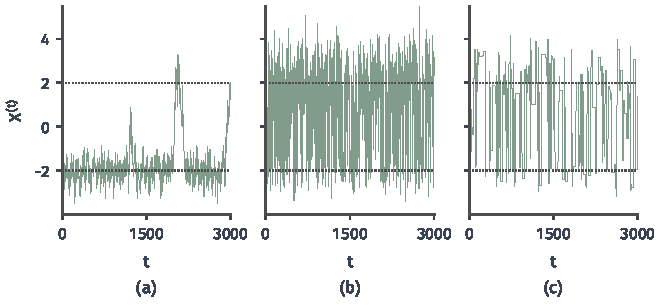
\includegraphics[width=112mm]{figures/07-probability/08-sampling-and-integration/matplotlib/sgen-rwmh-traces/figure.pdf}
  \caption{随机游走Metropolis在混合目标$0.3\,\mathcal{N}(-2,0.5^{2})+0.7\,\mathcal{N}(2,1)$上的轨迹，从$x=-2$出发，各$3000$步（种子$9$），虚线标出两个峰的位置。(a)$s=0.3$，接受率$0.83$；(b)$s=2.5$，接受率$0.47$；(c)$s=30$，接受率$0.064$，水平段是连续的拒绝。}
  \label{fig:sgen-rwmh-traces}
\end{BookInlineFigure}

三条链的转移都以同一个混合分布为不变分布，定理~\ref{thm:sgen-mh}对它们一视同仁。它们的差别全在“多快走遍目标”上，这是不变性之外的性质。每一步的成本是一次建议抽样、一次$\widetilde{p}$求值（当前点的值可以保存）和一个基础随机数。高维或尾部很重时，$\widetilde{p}$可能下溢为$0$或上溢，实际计算一律比较$\ln u_{\mathrm{a}}$与$\ln\widetilde{p}(y)-\ln\widetilde{p}(x)$加上建议比的对数。

\paragraph{建议必须能连通目标的支持}
不变性对任何建议都成立，包括那些根本到不了目标某些部分的建议。设目标是$[0,1]\cup[3,4]$上的均匀分布，建议是$y\sim\operatorname{Unif}(x-h,x+h)$。取$h=0.5$，从$x\in[0,1]$出发，候选落在$[x-0.5,x+0.5]\subset[-0.5,1.5]$中，凡是落在$[0,1]$之外的都有$\widetilde{p}(y)=0$而被拒绝，所以链永远留在$[0,1]$里。目标有一半质量在$[3,4]$上，链却一次也看不到。取$h=2.5$，候选可以越过长为$2$的空隙，链在两段之间往来（图~\ref{fig:sgen-mh-gap}）。

\begin{BookInlineFigure}
  \centering
  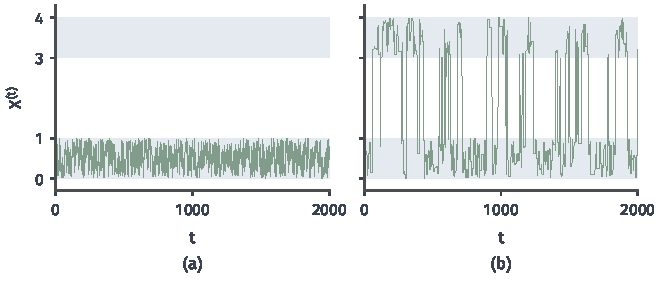
\includegraphics[width=112mm]{figures/07-probability/08-sampling-and-integration/matplotlib/sgen-mh-gap/figure.pdf}
  \caption{目标为$[0,1]\cup[3,4]$上的均匀分布（浅蓝带），建议为$\operatorname{Unif}(x-h,x+h)$，从$x=0.5$出发$2000$步（种子$10$）。(a)$h=0.5$：候选无法越过空隙，链停在$[0,1]$中，在$[3,4]$中的时间比例为$0$；(b)$h=2.5$：链在两段间往来，$[3,4]$中的时间比例为$0.39$，目标值为$0.5$。}
  \label{fig:sgen-mh-gap}
\end{BookInlineFigure}

这个例子中的失败在轨迹上一目了然，因为事先知道目标有两段。若不知道目标的形状，(a)的轨迹看起来是一条“混合良好”的链，在$[0,1]$上来回游走、接受率高达$0.75$，没有任何内部迹象提示还有一半质量没有访问。所以选择建议时，要从目标的结构出发论证它能连通支持，不能用接受公式的正确性或轨迹的外观代替这一论证。

\paragraph{独立建议}
另一种常用的建议是与当前状态无关的$q(y\mid x)=q(y)$，称为独立建议。记$w(x)=\widetilde{p}(x)/q(x)$，式~\eqref{eq:sgen-mh-acceptance}化为$\min\{1,w(y)/w(x)\}$：候选的权重比当前状态大就一定接受。它与拒绝采样用的是同一个比值，但不需要包络常数；代价是输出相关，而且若$q$在某处比目标轻得多，链一旦走到那里，$w(x)$很大，就会长时间被拒绝而停留。

\subsection{Gibbs采样}
\label{sec:sgen-gibbs}

多维目标的另一种局部信息是条件分布。设状态是$\bm{x}=(x_1,\dots,x_d)$，记$\bm{x}_{-i}$为去掉第$i$个坐标后的其余坐标。许多目标的联合分布难以直接抽样，但固定其余坐标后，第$i$个坐标的条件分布$\pi(\cdot\mid\bm{x}_{-i})$是一个熟悉的一维分布。这些条件分布称为完全条件分布。

\paragraph{单坐标更新}
保留其余坐标，只按完全条件分布重新抽第$i$个坐标，这一步的转移核记作$K_i$：从$\bm{x}$出发，新状态的第$i$个坐标服从$\pi(\cdot\mid\bm{x}_{-i})$，其余坐标与$\bm{x}$相同。轮流或随机地施行这些更新，就是\term{Gibbs采样}（Gibbs sampling）。

\begin{theorem}[单坐标更新保持目标]
\label{thm:sgen-gibbs}
设$\pi$是乘积空间上的分布，$\pi(\cdot\mid\bm{x}_{-i})$是给定其余坐标时第$i$个坐标的正则条件分布。则$\pi K_i=\pi$。
\end{theorem}

\begin{proof}
设$\bm{X}\sim\pi$，按$K_i$更新得到$\bm{X}'$，即$\bm{X}'_{-i}=\bm{X}_{-i}$，而给定$\bm{X}$时$X'_i$服从$\pi(\cdot\mid\bm{X}_{-i})$。新坐标只依赖$\bm{X}_{-i}$，旧的$X_i$在更新中被丢弃。于是$\bm{X}'_{-i}$的分布是$\pi$的边缘分布$\pi_{-i}$，给定$\bm{X}'_{-i}$时$X'_i$的条件分布是$\pi(\cdot\mid\bm{X}'_{-i})$。由第~\ref{chap:conditional-distributions}章，边缘分布与条件分布这一对确定了联合分布，它们恰好是$\pi$的边缘分布与条件分布，所以$\bm{X}'\sim\pi$。
\end{proof}

证明的直观是：更新前把$X_i$忘掉，剩下的$\bm{X}_{-i}$仍服从目标的边缘分布；再按正确的条件分布把$X_i$补回来，联合分布就复原了。也可以把单坐标更新看作建议为$q(\bm{y}\mid\bm{x})=\pi(y_i\mid\bm{x}_{-i})$的Metropolis--Hastings：此时$\bm{y}_{-i}=\bm{x}_{-i}$，比值
\[
  \frac{\pi(\bm{y})\,\pi(x_i\mid\bm{x}_{-i})}{\pi(\bm{x})\,\pi(y_i\mid\bm{x}_{-i})}=\frac{\pi_{-i}(\bm{x}_{-i})\pi(y_i\mid\bm{x}_{-i})\,\pi(x_i\mid\bm{x}_{-i})}{\pi_{-i}(\bm{x}_{-i})\pi(x_i\mid\bm{x}_{-i})\,\pi(y_i\mid\bm{x}_{-i})}=1,
\]
所以候选总被接受。

\paragraph{组合更新}
单坐标更新只动一个坐标，要让所有坐标都变化，需要把它们组合起来。按固定顺序依次施行$K_1,K_2,\dots,K_d$称为系统扫描，一轮的转移核是乘积$K_1K_2\cdots K_d$；每步以固定概率$c_i$随机选一个坐标更新，称为随机扫描，转移核是$\sum_ic_iK_i$，其中$c_i\ge0$、$\sum_ic_i=1$。两种组合都保持$\pi$：
\[
  \begin{gathered}
    \pi K_1K_2\cdots K_d=\pi K_2\cdots K_d=\dots=\pi,\\
    \pi\sum_ic_iK_i=\sum_ic_i\,\pi K_i=\sum_ic_i\pi=\pi.
  \end{gathered}
\]
随机扫描的条件是选择概率$c_i$固定，不能依赖当前状态。反例如下：设$\pi$是$\{0,1\}^{2}$上的均匀分布，规则为“$x_1=0$时更新第一个坐标，$x_1=1$时更新第二个坐标”。从$\pi$出发，$x_1=0$的一半质量更新$x_1$，其中一半变成$1$；$x_1=1$的一半质量只更新$x_2$，$x_1$保持为$1$。于是一步后
\[
  \mathbb{P}(X'_1=1)=\frac12\times\frac12+\frac12\times1=\frac34\ne\frac12 .
\]
每个$K_i$各自保持$\pi$，按状态挑选却把$x_1=1$的状态“锁住”了。

\paragraph{计算过程}
用二元高斯目标$\mathcal{N}(\bm{0},\bigl[\begin{smallmatrix}1&\rho\\\rho&1\end{smallmatrix}\bigr])$演示系统扫描，$\rho=0.8$。由第~\ref{chap:multivariate-distributions}章的高斯条件分布，两个完全条件分布是
\begin{equation}
  X_1\mid X_2=x_2\sim\mathcal{N}(\rho x_2,\,1-\rho^{2}),\qquad X_2\mid X_1=x_1\sim\mathcal{N}(\rho x_1,\,1-\rho^{2}).
  \label{eq:sgen-gibbs-gaussian}
\end{equation}

\needspace{6\baselineskip}
\paragraph{变量}
\begin{itemize}
  \item $(x_1,x_2)$：当前状态，每个坐标更新后立即覆盖。
  \item $z$：每次坐标更新使用的标准高斯数，由一个基础随机数经$\Phi^{-1}$得到。
\end{itemize}

\paragraph{初始化}
取一个初始状态。例中故意取在目标的边缘，$(x_1^{(0)},x_2^{(0)})=(2,2)$，以便看出链怎样走向中心。

\needspace{6\baselineskip}
\paragraph{每轮更新}
第$t+1$轮：
\begin{enumerate}
  \item \textbf{更新第一个坐标。}由式~\eqref{eq:sgen-gibbs-gaussian}，令
  \[
    x_1^{(t+1)}=\rho x_2^{(t)}+\sqrt{1-\rho^{2}}\,z .
  \]
  例中第一轮$z=\Phi^{-1}(0.37)\approx-0.3319$，
  \[
    x_1^{(1)}=0.8\times2+0.6\times(-0.3319)\approx1.4009 .
  \]

  \item \textbf{更新第二个坐标。}用刚得到的$x_1^{(t+1)}$，令
  \[
    x_2^{(t+1)}=\rho x_1^{(t+1)}+\sqrt{1-\rho^{2}}\,z' .
  \]
  例中第一轮$z'=\Phi^{-1}(0.80)\approx0.8416$，
  \[
    x_2^{(1)}=0.8\times1.4009+0.6\times0.8416\approx1.6257 .
  \]
  第二轮用$\Phi^{-1}(0.15)\approx-1.0364$与$\Phi^{-1}(0.62)\approx0.3055$，得到
  \[
    x_1^{(2)}\approx0.6787,\qquad x_2^{(2)}\approx0.7263 .
  \]

  \item \textbf{停止。}做满预定轮数后停止。
\end{enumerate}
最终得到状态序列$(2,2)$、$(1.4009,1.6257)$、$(0.6787,0.7263)$、\dots。每次只沿一个坐标轴移动，路径呈阶梯状。

\paragraph{相关性与移动速度}
相邻状态共用坐标，因而相关。在这个例子中可以算出相关的大小。把一轮的两步合起来，
\[
  X_1^{(t+1)}=\rho X_2^{(t)}+\sqrt{1-\rho^{2}}\,Z=\rho^{2}X_1^{(t)}+\rho\sqrt{1-\rho^{2}}\,Z''+\sqrt{1-\rho^{2}}\,Z,
\]
其中$Z''$是上一轮更新$X_2^{(t)}$所用的标准高斯数，$Z,Z''$与$X_1^{(t)}$独立。若链已处于目标分布，$\operatorname{Var}(X_1^{(t)})=1$，于是
\[
  \operatorname{Cov}\bigl(X_1^{(t+1)},X_1^{(t)}\bigr)=\rho^{2},
\]
逐轮迭代得到相隔$k$轮的相关系数为$\rho^{2k}$。$\rho=0.8$时每轮相关系数为$0.64$，几轮之后就基本忘记了起点；$\rho=0.99$时每轮为$0.98$，要约$35$轮相关系数才降到一半。

图~\ref{fig:sgen-gibbs-path}画出两种情形下前$20$轮的路径。目标沿对角线拉长时，每个完全条件分布都很窄，宽度为$\sqrt{1-\rho^{2}}$，链只能沿坐标轴迈小步，在狭长的山脊上缓慢挪动。这是Gibbs采样的典型弱点：坐标之间强相关时移动很慢，此时把强相关的坐标合成一块整体更新，或者换一套坐标，会有明显改善。

\begin{BookInlineFigure}
  \centering
  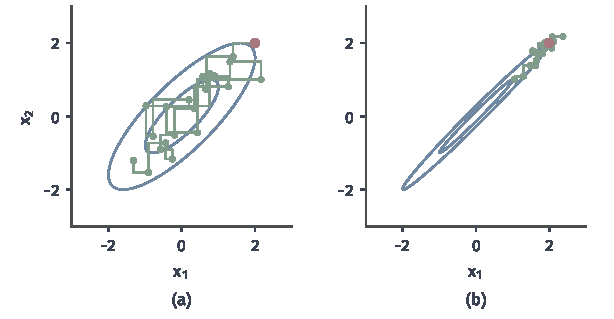
\includegraphics[width=104mm]{figures/07-probability/08-sampling-and-integration/matplotlib/sgen-gibbs-path/figure.pdf}
  \caption{二元高斯目标上的系统扫描Gibbs采样，从红点$(2,2)$出发$20$轮，前两轮使用正文中的随机数，其后的标准高斯数取自种子$12$。蓝色椭圆是目标的$1$倍与$2$倍等概率线，绿色阶梯是路径，绿点是每轮结束时的状态。(a)$\rho=0.8$，链很快进入中心并四处移动；(b)$\rho=0.99$，同样的随机数下链只沿山脊挪动了一小段。}
  \label{fig:sgen-gibbs-path}
\end{BookInlineFigure}

\paragraph{条件更新可能走不通}
Gibbs采样只沿坐标轴移动，目标的支持形状可能挡住去路。设目标是$[0,1]^{2}\cup[2,3]^{2}$上的均匀分布。当$x_2\in[0,1]$时，$x_1$的完全条件分布是$[0,1]$上的均匀分布，因为水平线$\{x_2=\text{常数}\}$只与下面的正方形相交；同理$x_1\in[0,1]$时$x_2$也只能在$[0,1]$中取值。从下面的正方形出发，链永远留在那里，尽管每一步都正确地保持了目标。若把两个正方形改成相互重叠的$[0,2]^{2}\cup[1,3]^{2}$，穿过重叠带的水平线同时碰到两个正方形，链就可以过去（图~\ref{fig:sgen-gibbs-reducible}）。

\begin{BookInlineFigure}
  \centering
  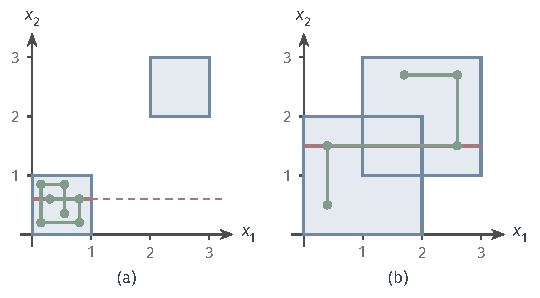
\includegraphics[width=91mm]{figures/07-probability/08-sampling-and-integration/tikz/sgen-gibbs-reducible/figure.pdf}
  \caption{支持形状对Gibbs采样的影响，目标是浅蓝区域上的均匀分布。(a)两个正方形在两个坐标方向上都不重叠，红色实线是$x_2=0.6$时$x_1$的条件分布所在区间，延长的红色虚线碰不到另一个正方形，绿色路径永远留在下方；(b)两个正方形部分重叠，红线$x_2=1.5$同时穿过两者，绿色路径经由它进入上方的正方形。}
  \label{fig:sgen-gibbs-reducible}
\end{BookInlineFigure}

每轮Gibbs采样的成本是$d$次条件抽样。完全条件分布是标准分布时，每次只需常数个基础随机数；不是标准分布时，每次条件抽样可能要用逆变换的数值反演、拒绝采样，甚至在这一坐标上做一步Metropolis--Hastings。后一种做法仍保持$\pi$，因为它是一个以$\pi(\cdot\mid\bm{x}_{-i})$为不变分布的一维更新，套上定理~\ref{thm:sgen-gibbs}的证明即可。

\subsection{Hamilton采样}
\label{sec:sgen-hmc}

随机游走建议和坐标更新都只能迈小步：步子大了接受率就低，坐标强相关时又只能沿轴挪动。若目标在欧氏空间上有光滑的正密度，梯度给出了“往哪里走概率不会掉太多”的信息。Hamilton采样借用力学中的运动方程，沿着保持总能量的轨道一次走出很远，再用接受判定修正数值误差\scite{pgm-sampling-neal2011}。

\paragraph{辅助动量与Hamilton量}
设目标为$\pi(\bm{x})\propto\exp(-U(\bm{x}))$，$\bm{x}\in\mathbb{R}^{d}$，其中$U=-\ln\widetilde{p}$二阶连续可微，称为势能。引入与$\bm{x}$同维、相互独立的辅助变量$\bm{p}\sim\mathcal{N}(\bm{0},\bm{I})$，称为动量。$(\bm{x},\bm{p})$的联合密度正比于
\begin{equation}
  \exp\bigl(-H(\bm{x},\bm{p})\bigr),\qquad H(\bm{x},\bm{p})=U(\bm{x})+\tfrac12\lVert\bm{p}\rVert_2^{2},
  \label{eq:sgen-hamiltonian}
\end{equation}
$H$称为Hamilton量，第二项是动能。联合密度分解为$\bm{x}$的因子与$\bm{p}$的因子之积，所以$\bm{x}$的边缘分布就是$\pi$：只要构造出保持联合分布的链，丢掉动量即可。

在相空间中沿Hamilton方程
\[
  \frac{\mathrm{d}\bm{x}}{\mathrm{d}t}=\bm{p},\qquad \frac{\mathrm{d}\bm{p}}{\mathrm{d}t}=-\nabla U(\bm{x})
\]
运动，有两条关键性质：$H$沿轨道守恒，相空间体积在流映射下保持不变，可参考\BookChapterRef{chap:ode-sensitivity}{卷六第4章“解的敏感性”}。$H$守恒意味着联合密度沿轨道不变，体积保持意味着把一块区域搬走时不需要Jacobian修正。轨道可以穿过目标的大片区域，同时停留在同一个密度水平上，这正是随机游走做不到的。

\paragraph{确定性提议的接受判定}
精确的Hamilton流一般解不出来，要用数值格式近似。先说明：任何满足两个条件的确定性映射，都可以配上一道接受判定而精确保持目标。

\begin{lemma}[对合映射的Metropolis修正]
\label{lem:sgen-involution}
设$\rho$是$\mathbb{R}^{m}$上的概率密度，$\Phi:\mathbb{R}^{m}\to\mathbb{R}^{m}$满足$\Phi\circ\Phi=\mathrm{id}$（对合），且保持体积（$\lvert\det D\Phi\rvert\equiv1$）。从$\bm{z}$出发，提议$\Phi(\bm{z})$，以概率$\min\{1,\rho(\Phi(\bm{z}))/\rho(\bm{z})\}$接受，否则留在$\bm{z}$。则$\rho$满足细致平衡，因而是不变分布。
\end{lemma}

\begin{proof}
从$\bm{z}$出发、被接受的移动所带的概率流密度为
\[
  m(\bm{z})=\rho(\bm{z})\min\Bigl\{1,\frac{\rho(\Phi(\bm{z}))}{\rho(\bm{z})}\Bigr\}=\min\bigl\{\rho(\bm{z}),\rho(\Phi(\bm{z}))\bigr\},
\]
$\rho(\bm{z})=0$时两边都取$0$。由$\Phi\circ\Phi=\mathrm{id}$，把$\bm{z}$换成$\Phi(\bm{z})$只是交换最小值中的两项，所以
\[
  m(\Phi(\bm{z}))=m(\bm{z}).
\]对可测集$A,B$，从$A$经接受的移动进入$B$的流量为
\[
  \int\mathbf{1}_{A}(\bm{z})\,\mathbf{1}_{B}(\Phi(\bm{z}))\,m(\bm{z})\,\mathrm{d}\bm{z}.
\]
作换元$\bm{z}=\Phi(\bm{w})$。由体积保持，体积元不变；由对合，$\Phi(\bm{z})=\bm{w}$；再由$m$在$\Phi$下不变，上式化为
\[
  \int\mathbf{1}_{A}(\Phi(\bm{w}))\,\mathbf{1}_{B}(\bm{w})\,m(\bm{w})\,\mathrm{d}\bm{w},
\]
这正是从$B$经接受的移动进入$A$的流量。被拒绝时留在原地，这部分流量对$A,B$对称。所以式~\eqref{eq:sgen-detailed-balance}成立，由引理~\ref{lem:sgen-detailed-balance}，$\rho$是不变分布。
\end{proof}

两个条件各有作用。对合使提议“可以原路返回”：从$\bm{z}$提议$\Phi(\bm{z})$，从$\Phi(\bm{z})$恰好提议回$\bm{z}$，正反两个方向成对出现。体积保持使换元时不出现Jacobian因子，接受概率只是密度之比。缺了体积保持，比值中还要乘上$\lvert\det D\Phi(\bm{z})\rvert$。

\paragraph{蛙跳格式}
求解Hamilton方程的\term{蛙跳格式}（leapfrog scheme）以步长$\varepsilon$做三个子步：
\begin{equation}
  \bm{p}_{1/2}=\bm{p}-\frac{\varepsilon}{2}\nabla U(\bm{x}),\qquad
  \bm{x}'=\bm{x}+\varepsilon\,\bm{p}_{1/2},\qquad
  \bm{p}'=\bm{p}_{1/2}-\frac{\varepsilon}{2}\nabla U(\bm{x}'),
  \label{eq:sgen-leapfrog}
\end{equation}
记这一步为$\Psi_{\varepsilon}:(\bm{x},\bm{p})\mapsto(\bm{x}',\bm{p}')$。

它保持体积：三个子步各自只改变一组变量，改变量只依赖另一组变量，例如第一步$(\bm{x},\bm{p})\mapsto(\bm{x},\bm{p}-\tfrac{\varepsilon}{2}\nabla U(\bm{x}))$的Jacobian矩阵是分块下三角的，对角块都是单位矩阵，行列式为$1$。三个这样的映射复合，行列式仍为$1$。

它在动量反转下可逆。记$F(\bm{x},\bm{p})=(\bm{x},-\bm{p})$。从$(\bm{x}',-\bm{p}')$再做一步$\Psi_{\varepsilon}$，三个子步依次给出
\[
  \begin{aligned}
    -\bm{p}'-\tfrac{\varepsilon}{2}\nabla U(\bm{x}')&=-\bm{p}_{1/2},\\
    \bm{x}'+\varepsilon(-\bm{p}_{1/2})&=\bm{x},\\
    -\bm{p}_{1/2}-\tfrac{\varepsilon}{2}\nabla U(\bm{x})&=-\bm{p},
  \end{aligned}
\]
第一行用到式~\eqref{eq:sgen-leapfrog}的第三式，第二、三行用到第二式和第一式。所以先走一步、反转、再走一步，得到的是$(\bm{x},-\bm{p})$，即$\Psi_{\varepsilon}F\Psi_{\varepsilon}=F$。由$F\circ F=\mathrm{id}$，这等价于$F\Psi_{\varepsilon}F=\Psi_{\varepsilon}^{-1}$。连做$L$步时，
\[
  F\Psi_{\varepsilon}^{L}F=(F\Psi_{\varepsilon}F)^{L}=\Psi_{\varepsilon}^{-L},
\]
所以$\Phi=F\circ\Psi_{\varepsilon}^{L}$满足$\Phi\circ\Phi=\mathrm{id}$，并且保持体积。精确的Hamilton流有同样两条性质，蛙跳格式在离散后仍完整保留了它们，失去的只是$H$的守恒。

\paragraph{完整的一步}
\term{Hamilton采样}（Hamiltonian Monte Carlo）的一步由两部分组成：
\begin{enumerate}
  \item \textbf{刷新动量。}丢弃旧的动量，重新抽$\bm{p}\sim\mathcal{N}(\bm{0},\bm{I})$。在联合分布下$\bm{p}$与$\bm{x}$独立，这一步就是对$\bm{p}$的一次Gibbs更新，由定理~\ref{thm:sgen-gibbs}，它保持联合分布。

  \item \textbf{轨道提议与修正。}从$(\bm{x},\bm{p})$出发做$L$步蛙跳，再反转动量，得到
  \[
    (\bm{x}^{*},\bm{p}^{*})=F\Psi_{\varepsilon}^{L}(\bm{x},\bm{p}),
  \]
  以概率
  \begin{equation}
    \min\Bigl\{1,\ \exp\bigl(H(\bm{x},\bm{p})-H(\bm{x}^{*},\bm{p}^{*})\bigr)\Bigr\}
    \label{eq:sgen-hmc-accept}
  \end{equation}
  接受$\bm{x}^{*}$，否则保留$\bm{x}$。由引理~\ref{lem:sgen-involution}（取$\rho\propto\mathrm{e}^{-H}$），这一步也保持联合分布。
\end{enumerate}
两步复合仍保持联合分布，于是$\bm{x}$的边缘分布$\pi$不变。式~\eqref{eq:sgen-hmc-accept}只用到$U$的值差，归一化常数照样约掉。

四个组成部分各司其职。刷新动量改变能量水平：若不刷新，链只在一条近似的能量等值面上移动，无法到达其他密度水平。蛙跳格式的可逆与保体积使接受概率只含能量差。动量反转把提议变成对合，满足引理的条件；下一步开始时动量会被重新抽取，而$\mathcal{N}(\bm{0},\bm{I})$关于$\bm{p}\mapsto-\bm{p}$对称，所以实际程序中常省去这一反转。接受判定修正离散化误差：精确流下$H$守恒，接受概率为$1$，蛙跳的能量误差越小，接受率越高。

\paragraph{计算过程}
用一维标准高斯目标演示，$U(x)=x^{2}/2$，$\nabla U(x)=x$，步长$\varepsilon=0.5$，每次提议走$L=2$步。

\needspace{6\baselineskip}
\paragraph{变量}
\begin{itemize}
  \item $x$：当前位置；$p$：本次刷新的动量。
  \item $(x_{\ell},p_{\ell})$：蛙跳第$\ell$步后的位置与动量，$\ell=0,\dots,L$。
  \item $\Delta H$：轨道终点与起点的能量差。
\end{itemize}

\paragraph{初始化}
给定当前位置。例中$x=1$。

\needspace{6\baselineskip}
\paragraph{每轮更新}
\begin{enumerate}
  \item \textbf{刷新动量。}抽$p\sim\mathcal{N}(0,1)$。例中由$u=0.80$得$p=\Phi^{-1}(0.80)\approx0.8416$，于是
  \[
    H(x_0,p_0)=\frac{1^{2}}{2}+\frac{0.8416^{2}}{2}\approx0.8542 .
  \]

  \item \textbf{蛙跳$L$步。}按式~\eqref{eq:sgen-leapfrog}迭代。例中第一步
  \[
    \begin{aligned}
      p_{1/2}&=0.8416-0.25\times1=0.5916,\\
      x_1&=1+0.5\times0.5916=1.2958,\\
      p_1&=0.5916-0.25\times1.2958\approx0.2677 .
    \end{aligned}
  \]
  第二步
  \[
    \begin{aligned}
      p_{3/2}&\approx0.2677-0.25\times1.2958=-0.0563,\\
      x_2&\approx1.2958+0.5\times(-0.0563)=1.2677,\\
      p_2&\approx-0.0563-0.25\times1.2677=-0.3732 .
    \end{aligned}
  \]

  \item \textbf{反转并计算能量差。}令$p^{*}=-p_2$，它不改变动能。例中
  \[
    H(x_2,p^{*})=\frac{1.2677^{2}}{2}+\frac{0.3732^{2}}{2}\approx0.8731,\qquad \Delta H\approx0.0190 .
  \]

  \item \textbf{判定。}由式~\eqref{eq:sgen-hmc-accept}，接受概率为$\min\{1,\mathrm{e}^{-\Delta H}\}$。例中$\mathrm{e}^{-0.0190}\approx0.9812$，取基础随机数$u=0.37$，接受，新位置为$1.2677$。
\end{enumerate}
最终一次迭代用到$x_0,x_1,x_2$三处的梯度（$x_1$处的梯度在两步之间重复使用）和两个基础随机数，位置从$1$移到$1.2677$。能量只变了约$0.019$，所以几乎必然接受。

\paragraph{步长与轨道长度}
步长决定能量误差。对这个一维例子，式~\eqref{eq:sgen-leapfrog}是线性映射，代入$\nabla U(x)=x$可得
\[
  \begin{bmatrix}x'\\p'\end{bmatrix}=
  \begin{bmatrix}1-\varepsilon^{2}/2&\varepsilon\\-\varepsilon(1-\varepsilon^{2}/4)&1-\varepsilon^{2}/2\end{bmatrix}
  \begin{bmatrix}x\\p\end{bmatrix}.
\]
矩阵的行列式为$1$，迹为$2-\varepsilon^{2}$。$0<\varepsilon<2$时迹的绝对值小于$2$，两个特征值是单位圆上的一对共轭复数，迭代点在一个椭圆上转动，能量误差有界；$\varepsilon>2$时有一个特征值的绝对值大于$1$，轨道按指数发散，接受率趋于零。若目标的标准差为$\sigma$，同样的计算给出稳定条件$\varepsilon<2\sigma$；多维时由最窄的方向决定。

图~\ref{fig:sgen-leapfrog}(a)画出$\varepsilon=0.5$与$\varepsilon=1.8$的轨道，前者紧贴精确的圆形轨道，后者被拉成扁椭圆。(b)是固定轨道总长约为$3$时，轨道上最大能量误差随$\varepsilon$的变化，在稳定范围内大致与$\varepsilon^{2}$成正比。对一般的光滑$U$，固定轨道长度时能量误差为$O(\varepsilon^{2})$，证明要用到数值积分的误差分析，这里只用图中的数值说明。

\begin{BookInlineFigure}
  \centering
  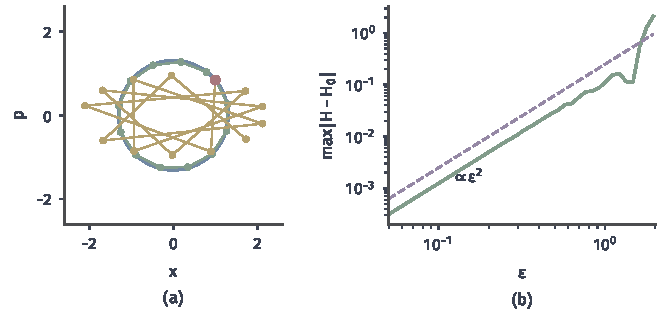
\includegraphics[width=112mm]{figures/07-probability/08-sampling-and-integration/matplotlib/sgen-leapfrog/figure.pdf}
  \caption{标准高斯目标的蛙跳格式，起点为红点$(x,p)=(1,\Phi^{-1}(0.8))$。(a)蓝线是精确的Hamilton轨道（能量等值线），绿色是$\varepsilon=0.5$的$12$步，黄色是$\varepsilon=1.8$的$12$步；(b)轨道总长约为$3$（$L=\operatorname{round}(3/\varepsilon)$）时轨道上的最大能量误差，紫色虚线是斜率为$2$的参考线。}
  \label{fig:sgen-leapfrog}
\end{BookInlineFigure}

轨道长度$L\varepsilon$决定一次能走多远。太短时与随机游走无异；太长时轨道可能绕回起点附近，例如标准高斯的精确轨道周期为$2\pi$，走满一周等于白走。每次提议的成本是$L$次梯度计算，比较方法时应在相同的梯度或密度计算次数下比较。图~\ref{fig:sgen-hmc-rw}在相关系数为$0.95$的二元高斯目标上做了这样的比较：$200$次密度计算的随机游走Metropolis（接受率$0.69$）还在山脊的一端徘徊，$200$次梯度计算的Hamilton采样（$20$次提议，每次$10$步，接受率$0.85$）已在整个椭圆上来回。

\begin{BookInlineFigure}
  \centering
  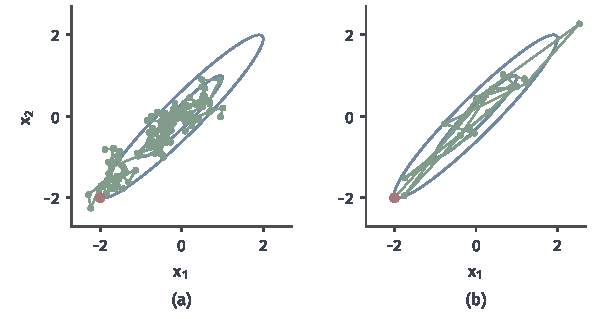
\includegraphics[width=104mm]{figures/07-probability/08-sampling-and-integration/matplotlib/sgen-hmc-rw/figure.pdf}
  \caption{相关系数$0.95$的二元高斯目标，从红点$(-2,-2)$出发，计算量相同。(a)随机游走Metropolis，步长$0.25$，$200$步；(b)Hamilton采样，$\varepsilon=0.18$、$L=10$，$20$次提议。两者都用种子$13$，蓝色椭圆是$1$倍与$2$倍等概率线。}
  \label{fig:sgen-hmc-rw}
\end{BookInlineFigure}

Hamilton采样的适用范围也由它的条件划定。它需要欧氏空间上光滑、处处为正的密度和可以计算的梯度，离散变量或有硬边界的支持都要另行处理。多峰目标中，两个峰之间的低密度区要靠刷新动量时偶尔得到的高能量才能越过，峰间隔得远时同样会长期困在一个峰中。

\section{生成结果的核验}
\label{sec:sgen-checks}

一个生成程序写好之后，怎样确认它给出的是想要的东西？前面几节其实已经区分了两类要核对的性质：直接生成要核对每个样本的分布及样本之间的独立性，链式更新要核对目标是否为不变分布以及链能否走遍目标。此外，实际程序与数学方法之间还隔着停止规则、有限精度和数值近似，它们各自会引入偏差。本节逐项说明怎样核对，以及经验检查能说明什么、不能说明什么。

\paragraph{直接生成：分布与独立性}
直接生成的正确性有完整的数学判据：输出分布满足式~\eqref{eq:sgen-correct-law}。前几节对每种方法都给出了这样的证明，核验时要逐条对照证明用到的条件是否在程序中成立，例如分位数是否对所有$u$有误差界、包络常数是否真正满足式~\eqref{eq:sgen-envelope}、混合采样的两步是否使用了不同的随机数。

独立性来自输入：每个样本只使用自己的一组基础随机数，组与组互不重叠。核对时要看程序是否在样本之间共用了状态，例如为了“节省”而把上一个样本剩余的随机数或中间结果留给下一个样本。只要输入不重叠，同分布且独立就有保证，样本个数再多也不会产生相关。

\paragraph{链式更新：不变性、可达性与相关性}
链的不变性同样可以证明，并且可以对小问题做精确的数值核对。把程序中的接受规则原样用在一个有限状态的小目标上（例如第~\ref{sec:sgen-mh}节的三状态目标），按程序逻辑写出完整的转移矩阵$\bm{K}$，直接计算$\pi\bm{K}-\pi$。它应在舍入误差以内为零。这种核对不依赖任何模拟，能发现遗漏建议比、遗漏拒绝时的重复记录之类的错误：前面已经算出，遗漏建议比会把不变分布变成$(2/15,2/3,1/5)$。

可达性无法用这种方式核对，它是关于整个目标支持的全局性质，要从目标的结构论证，例如说明建议分布能以正概率从任一点走到任一个正概率区域附近。第~\ref{sec:sgen-mh}节与第~\ref{sec:sgen-gibbs}节的两个反例都是每一步都正确、整体却走不通的情形。

即使链从目标分布出发，各个状态的边缘分布都是$\pi$，状态之间也一般相关，不能当作独立样本。图~\ref{fig:sgen-checks}(c)是二元高斯Gibbs采样中$X_1$的样本自相关，与第~\ref{sec:sgen-gibbs}节算出的$\rho^{2k}$一致：$\rho=0.99$时相隔$40$轮仍有约$0.5$的相关。相关性对积分误差的影响是下一章的内容，这里只需记住：链的输出不满足独立样本的假设。

\paragraph{停止规则带来的偏差}
理论上的方法常常假设可以无限地做下去，程序却必须停下来，停止的方式会改变输出分布。

拒绝采样理论上试到接受为止。若程序为了限制时间，最多试$T$次，全部失败时返回最后一个候选，输出就不再服从$\pi$。记接受率为$a$，前$n-1$次失败、第$n$次接受的概率是$(1-a)^{n-1}a$，接受的样本服从$\pi$；$T$次全部失败的概率是$(1-a)^{T}$，此时返回的候选服从“候选在被拒绝条件下”的分布。由定理~\ref{thm:sgen-rejection}的计算，候选被拒绝且落在$A$中的概率是$\int_{A}q-\tfrac1M\int_{A}\widetilde{p}$，记其条件分布为$R$。于是输出分布为
\begin{equation}
  \bigl(1-(1-a)^{T}\bigr)\,\pi+(1-a)^{T}R .
  \label{eq:sgen-capped-rejection}
\end{equation}
偏差的权重$(1-a)^{T}$随$T$几何下降，但永远不为零。以$\operatorname{Beta}(2,2)$的例子计算，$a=2/3$，$R$的密度为
\[
  \frac{1-4x(1-x)}{1/3}=3(1-2x)^{2}.
\]
$T=1$时式~\eqref{eq:sgen-capped-rejection}给出$\tfrac23\cdot6x(1-x)+\tfrac13\cdot3(1-2x)^{2}=1$，即输出就是建议分布本身，这与“只试一次就交出候选”的直觉一致（图~\ref{fig:sgen-capped-rejection}）。

\begin{BookInlineFigure}
  \centering
  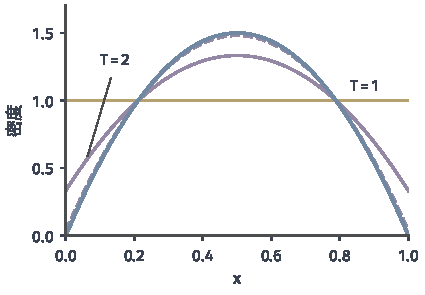
\includegraphics[width=72mm]{figures/07-probability/08-sampling-and-integration/matplotlib/sgen-capped-rejection/figure.pdf}
  \caption{最多试$T$次的拒绝采样的输出密度，目标$\operatorname{Beta}(2,2)$，建议$\operatorname{Unif}(0,1)$，$M=1/4$。黄线$T=1$（等于建议分布），紫色实线$T=2$，紫色虚线$T=4$，蓝线是目标$6x(1-x)$。偏差权重为$(1/3)^{T}$。}
  \label{fig:sgen-capped-rejection}
\end{BookInlineFigure}

链式更新也有同样的问题。从$\mu_0$出发运行$t$步，$X^{(t)}$的分布是$\mu_0K^{t}$，一般不等于$\pi$。第~\ref{sec:sgen-invariance}节的三状态例子从状态$1$出发，$5$步后的分布是$(0.219,0.5,0.281)$，离$\pi=(0.2,0.5,0.3)$还有可见的差距。“等到轨迹看起来稳定再开始记录”是一种依赖于已生成数据的停止规则，它本身也会改变被记录状态的分布。这些偏差有多大、怎样控制，是下一章讨论链初值影响时的主题。

\paragraph{有限精度与数值近似}
每一种数值近似都在数学方法与程序输出之间插入了一个误差，核验时要逐个列出。逆变换中的数值反演按引理~\ref{lem:sgen-inversion-error}改变输出的分布函数，误差界必须对全部$u$成立；协方差因子的舍入误差改变输出的协方差。链式更新中，接受比值若直接用密度相除，可能出现下溢后的$0/0$，应改用对数。Hamilton采样中步长超过稳定范围时轨道发散，表现为能量差变成很大的数或非数值，程序应把它作为拒绝处理并报告，而不是悄悄跳过这一步：跳过等于改变了转移核。

这些近似之外，还有基础随机数本身与理想模型的差距（第~\ref{sec:sgen-uniform}节）。近似生成造成的偏差不会随样本数增加而消失，它与样本数决定的随机波动是两种不同的误差，下一章将分开评价。

\paragraph{经验检查的作用与边界}
直方图、样本矩、自相关与轨迹图是最常用的经验检查。它们能发现问题，却不能证明正确。图~\ref{fig:sgen-checks}给出三种情形。

\begin{BookInlineFigure}
  \centering
  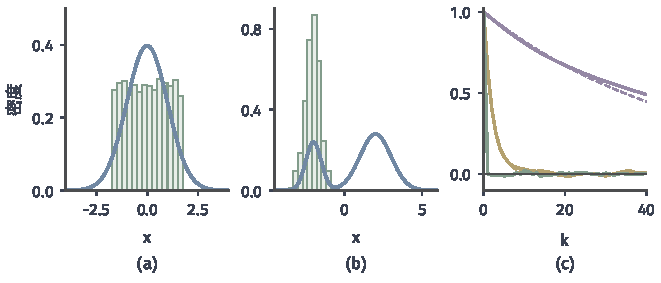
\includegraphics[width=112mm]{figures/07-probability/08-sampling-and-integration/matplotlib/sgen-checks/figure.pdf}
  \caption{经验检查能看出什么。(a)$\operatorname{Unif}(-\sqrt3,\sqrt3)$的$5000$个样本（种子$14$），样本均值$0.006$、方差$1.007$，与$\mathcal{N}(0,1)$（蓝线）的前两阶矩相同，直方图却明显不同；(b)第~\ref{sec:sgen-mh}节步长$0.3$的随机游走Metropolis的前$1000$个状态，直方图是一个干净的单峰，蓝线是混合目标；(c)二元高斯Gibbs采样中$X_1$的样本自相关（$20000$轮，种子$15$），黄线$\rho=0.8$，紫线$\rho=0.99$，虚线是$\rho^{2k}$，绿线是独立样本。}
  \label{fig:sgen-checks}
\end{BookInlineFigure}

(a)说明低阶矩相符不能说明分布正确：均匀分布$\operatorname{Unif}(-\sqrt3,\sqrt3)$的均值为$0$、方差为$1$，与标准高斯相同。若某个“高斯生成器”实际输出的是它，只检查均值与方差永远发现不了，直方图则一眼可见。反过来，直方图只比较到分箱的分辨率，比分箱更细的偏差（例如第~\ref{sec:sgen-transform}节固定轮数二分法造成的离散化）以及远处尾部的偏差，直方图也看不出来。

(b)说明经验检查只能看到已经访问过的区域。链的前$1000$个状态全部在左峰附近，直方图形状规则，与左峰的密度相符；单看这批状态，没有任何迹象提示右边还有一个占$70\%$质量的峰。只有事先知道目标有两个峰，才能看出问题。同理，从不同初值出发的多条链若都没有找到某个区域，它们彼此一致也不能说明那个区域不存在。

(c)说明自相关可以量出链的“记性”有多长，却不能说明链已经走遍了目标：一条困在单峰中的链，在峰内的自相关可能很快衰减。

所以经验检查的作用是排除明显的错误：它们发现的偏差是真实的，没有发现偏差则不构成证明。正确性的依据仍是前面各节的证明，加上对可达性的结构论证；经验检查在此基础上补充核对程序是否忠实地实现了证明中的方法。

\section{本章小结}
\label{sec:sgen-summary}

本章从独立均匀的基础随机数出发，回答了章首的问题：怎样把它们加工成给定分布的样本，以及加工结果是什么性质的样本。方法的选择取决于目标分布提供了哪些可以计算的信息。表~\ref{tab:sgen-methods}把各种方法放在一起比较。

\begin{BookInlineTable}
  \centering
  \small
  \begin{tabular}{@{}llll@{}}
    \toprule
    方法 & 需要的信息 & 输出 & 主要成本与失效 \\
    \midrule
    逆变换 & 分位数或可反演的$F$ & 独立样本 & 数值反演误差、尾部截断 \\
    仿射高斯 & 协方差因子 & 独立样本 & 一次分解，奇异时退化 \\
    分步生成 & 成分或条件分布 & 独立样本 & 各步须用不同随机数 \\
    拒绝采样 & $\widetilde{p}$、建议、包络$M$ & 独立样本 & 平均$M/Z$次试验 \\
    MH & $\widetilde{p}$、建议密度 & 相关的链 & 步长取舍、支持连通 \\
    Gibbs & 完全条件分布 & 相关的链 & 强相关时慢、支持形状 \\
    Hamilton & $\nabla U$、光滑正密度 & 相关的链 & 每步$L$次梯度、步长稳定 \\
    \bottomrule
  \end{tabular}
  \caption{采样生成方法的比较。前四种输出服从目标分布的独立样本；后三种输出以目标为不变分布的链，状态相关，能否走遍目标需另行论证。}
  \label{tab:sgen-methods}
\end{BookInlineTable}

直接生成的三种机制都以推前为核心。变量变换把易抽变量送到目标，正确性由原像规则或可逆映射的换元公式验证；逆变换对一切实值分布成立，分位数可以解析计算时最简便，需要数值反演时，引理~\ref{lem:sgen-inversion-error}说明逐点误差$\delta$怎样把分布函数夹在$F(x\pm\delta)$之间，前提是误差界对所有$u$都成立。高斯样本由独立标准坐标经仿射变换得到，协方差奇异时输出落在低维子空间上，没有密度但分布正确。

分步生成依靠全概率公式与链式分解，关键条件是各步使用互不重叠的随机数；输入独立并不意味着同一样本的坐标独立。拒绝采样只需未归一化密度与有效包络，接受样本精确服从目标，代价是平均$M/Z$次试验，在高维中常因包络过松而无法使用。只要每次都用一组新的基础随机数从头生成，以上方法都给出独立同分布的目标样本。

链式更新换了一种思路：放弃一次造出完整样本，转而构造以目标为不变分布的转移。不变性是一个代数条件，细致平衡是验证它的便利充分条件。Metropolis--Hastings用接受概率$\min\{1,\widetilde{p}(y)q(x\mid y)/(\widetilde{p}(x)q(y\mid x))\}$平衡双向概率流，其中建议比修正了建议本身的偏向，归一化常数约去；Gibbs采样按完全条件分布逐坐标更新，选坐标的概率不能依赖当前状态；Hamilton采样借助辅助动量和保持体积、可逆的蛙跳格式走出远距离的提议，再用能量差修正离散误差。三者都只证明了不变性。

不变性不保证从任意初值到达目标：停在原地的转移、无法越过空隙的建议、被支持形状挡住的坐标更新都是反例。即使从目标出发，链的状态也相互相关。

核验生成结果时，要分别检查输出分布或不变性的证明、链的可达性、停止规则和数值近似带来的偏差。直方图和样本矩能发现错误，但看不到从未访问的区域，也不能代替证明。

链的长期行为，即在什么条件下分布收敛、时间平均收敛以及收敛有多快，由卷九讨论。下一章转向用这些样本计算积分：独立样本平均的误差、近似生成造成的偏差、链初值的影响，以及相关样本平均的方差，都将在那里分别评价。


\chapter{积分误差}
\label{chap:monte-carlo-integration-error}

积分$I=\int_0^1\mathrm{e}^{u}\,\mathrm{d}u$有公式，$I=\mathrm{e}-1\approx1.7183$，正好用来检验随机计算。取五个均匀随机数，把$\mathrm{e}^{u}$在这五点的值平均，得到的数大约是$1.82$；换五个随机数，又得到另一个数。这个数离$1.7183$有多远？取多少个点才能保证误差小于$0.01$？如果生成随机数的程序本身有近似，或者样本来自一条逐步游走的Markov链，答案又会怎样变化？

第~\ref{chap:sample-generation}章解决了“怎样得到样本”。本章假定分布和被积函数都已给定，研究用样本平均代替积分时产生的误差。误差有两个来源：一是样本的实际规律与目标不符造成的系统偏离，二是有限个随机样本带来的波动。前者不会因样本增多而消失，后者随样本增多而缩小，但缩小的速度取决于矩条件和样本之间的依赖。

全章按样本的来源推进。先对独立且精确的样本给出有限样本概率界和渐近误差区间；再分别处理近似生成造成的偏差、Markov链初值造成的偏差，以及链样本相关性对方差的影响；随后说明链平均的误差区间需要哪些条件，运行诊断能发现什么、不能保证什么。最后讨论一次产生一组相关点的方法，把整组的独立重复当作观测单位来估计误差，为第~\ref{chap:variance-reduction}章的抽样设计做准备。

全章使用第~\ref{chap:laws-of-large-numbers}章的大数律、第~\ref{chap:central-limit-theorem}章的中心极限定理、第~\ref{chap:weak-convergence-of-distributions}章的Slutsky定理，以及第~\ref{chap:distribution-comparison}章的总变差距离。

\section{积分的样本估计}
\label{sec:mcerr-estimator}

用随机样本算积分，首先要说清楚算的是什么、用什么去算，以及“误差”指的是哪一个量与哪一个量之差。设$\pi$是取值空间$\mathcal{X}$上的概率分布，$f\colon\mathcal{X}\to\mathbb{R}$可测且$\mathbb{E}_{\pi}\lvert f\rvert<\infty$。要计算的是
\begin{equation}
 I=\mathbb{E}_{\pi}[f]=\int_{\mathcal{X}}f(x)\,\pi(\mathrm{d}x) .
 \label{eq:mcerr-target}
\end{equation}
这里$\pi$与$f$都已完全给定，$I$是一个确定的数，只是不便用公式或网格求积算出。

\paragraph{样本平均}
设某个生成程序产生了$X_1,\dots,X_N$。它们的联合规律由程序决定，称为\emph{实际生成规律}；它可能是$N$个独立的$\pi$样本，也可能各项相关，甚至各项的分布都与$\pi$不同。用函数值的平均
\begin{equation}
 \hat{I}_N=\frac{1}{N}\sum_{i=1}^{N}f(X_i)
 \label{eq:mcerr-estimator}
\end{equation}
近似$I$，这种用随机样本的平均计算积分的方法称为\term{Monte Carlo方法}（Monte Carlo method），$\hat{I}_N$称为$I$的Monte Carlo估计。第~\ref{chap:laws-of-large-numbers}章在四分之一圆的面积上已经用过它。

$\hat{I}_N$中的随机性来自计算过程本身：换一组随机数，结果就会变。这与统计推断不同。统计推断里$\pi$未知，样本是观测到的数据，要由数据推断总体，可参考\BookChapterRef{chap:parametric-statistical-inference}{卷八第1章“参数化统计推断”}。本章的$\pi$是已知的，我们可以随意重新生成样本，问题只在于计算的精度。

\paragraph{偏差与波动}
误差$\hat{I}_N-I$是一个随机变量。设每个$f(X_i)$在实际生成规律下都可积，于是$\mathbb{E}[\hat{I}_N]$有定义，误差可以分成两部分：
\begin{equation}
 \hat{I}_N-I=\underbrace{\bigl(\mathbb{E}[\hat{I}_N]-I\bigr)}_{\text{偏差}}+\underbrace{\bigl(\hat{I}_N-\mathbb{E}[\hat{I}_N]\bigr)}_{\text{随机波动}} .
 \label{eq:mcerr-split}
\end{equation}
第一部分记作$b_N=\mathbb{E}[\hat{I}_N]-I$，称为偏差，它是确定的数，表示重复计算无穷多次以后平均结果离目标多远。第二部分均值为零，表示单次计算围绕自己的平均值摆动多少。$b_N=0$时称$\hat{I}_N$无偏。

偏差只依赖各个$X_i$各自的分布，与它们之间是否独立无关。由期望的线性，
\[
 \mathbb{E}[\hat{I}_N]=\frac1N\sum_{i=1}^{N}\mathbb{E}[f(X_i)] .
\]
所以只要每个$X_i$都服从$\pi$，不论它们怎样相关，$\hat{I}_N$都无偏。反过来，样本之间的依赖只影响第二部分。后面几节正是按这个分工展开的：第~\ref{sec:mcerr-approx}节与第~\ref{sec:mcerr-initial}节处理各项分布偏离$\pi$造成的偏差，第~\ref{sec:mcerr-correlated}节处理依赖对波动的影响。

两部分合在一起时，最常用的尺度是均方误差。

\begin{theorem}[均方误差的分解]
\label{thm:mcerr-mse}
设$\mathbb{E}[\hat{I}_N^{2}]<\infty$。则
\begin{equation}
 \mathbb{E}\bigl[(\hat{I}_N-I)^{2}\bigr]=b_N^{2}+\operatorname{Var}(\hat{I}_N) .
 \label{eq:mcerr-mse}
\end{equation}
\end{theorem}

\begin{proof}
记$m=\mathbb{E}[\hat{I}_N]$。由式~\eqref{eq:mcerr-split}，把平方展开，
\[
 (\hat{I}_N-I)^{2}=(m-I)^{2}+2(m-I)(\hat{I}_N-m)+(\hat{I}_N-m)^{2} .
\]
二阶矩有限保证三项都可积。取期望，中间一项的期望是$2(m-I)\,\mathbb{E}[\hat{I}_N-m]=0$，第一项是常数$b_N^{2}$，最后一项是方差。
\end{proof}

均方根误差$\sqrt{\mathbb{E}[(\hat{I}_N-I)^{2}]}$与$\hat{I}_N$同单位，便于与要求的精度比较。可以把计算想成打靶：偏差是瞄准器装歪了，每一枪都朝同一个方向偏；波动是手抖，弹着点围绕瞄准点散开。打得越多，弹着点的平均越接近瞄准点，却不会自动回到靶心。这个比喻在一点上不准：打靶时看得见靶心，算积分时$I$恰恰未知，所以偏差无法从结果本身读出来，只能从生成规律分析出来。

\paragraph{两个例子}
先看本章开头的积分$I=\int_0^1\mathrm{e}^{u}\,\mathrm{d}u$，即$\pi=\operatorname{Unif}(0,1)$，$f(u)=\mathrm{e}^{u}$。取五个均匀随机数
\[
 u_1=0.37,\quad u_2=0.81,\quad u_3=0.12,\quad u_4=0.55,\quad u_5=0.94 .
\]
对应的函数值是
\[
 1.4477,\quad 2.2479,\quad 1.1275,\quad 1.7333,\quad 2.5600 ,
\]
平均为$\hat{I}_5=1.8233$，误差为$1.8233-1.7183=0.1050$。单看这一个数，分不出误差来自偏差还是波动；要回答这个问题，需要知道$\hat{I}_N$作为随机变量的分布。

第二个例子显示偏差。设目标是$X\sim\operatorname{Exp}(1)$的均值，$f(x)=x$，$I=1$。由第~\ref{chap:sample-generation}章的逆分位数方法，$X=-\ln(1-U)$精确服从$\operatorname{Exp}(1)$。假设某个程序为了避免输出过大，把结果截到$T=2$，实际输出$\tilde{X}=\min\{X,2\}$。由尾概率公式，
\[
 \mathbb{E}[\min\{X,T\}]=\int_0^{T}\mathbb{P}(X>t)\,\mathrm{d}t=\int_0^{T}\mathrm{e}^{-t}\,\mathrm{d}t=1-\mathrm{e}^{-T} .
\]
$T=2$时它等于$0.8647$，所以截断程序的偏差是$b_N=-\mathrm{e}^{-2}=-0.1353$，对每个$N$都一样。

图~\ref{fig:mcerr-bias-spread}把两个程序各运行$20000$次，每次$N=20$。精确程序的估计以$I=1$为中心，样本标准差为$0.2247$；截断程序的估计以$0.8651$为中心，标准差只有$0.1488$，因为截断去掉了大值。按式~\eqref{eq:mcerr-mse}计算，两者的均方误差分别是
\[
 \frac{1}{20}=0.0500,\qquad 0.1353^{2}+\frac{0.4403}{20}=0.0183+0.0220=0.0403 ,
\]
其中$0.4403$是$\min\{X,2\}$的方差（第~\ref{sec:mcerr-approx}节给出计算）。在$N=20$时有偏的程序均方误差反而更小。这说明均方误差一个数掩盖了误差的结构：样本增多以后，波动项缩小而偏差项不变，两者的比较会颠倒过来。

\begin{BookInlineFigure}
 \centering
 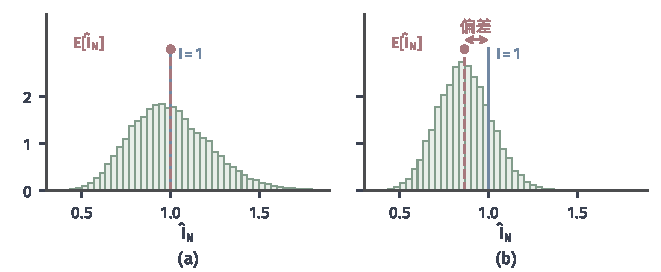
\includegraphics[width=112mm]{figures/07-probability/08-sampling-and-integration/matplotlib/mcerr-bias-spread/figure.pdf}
 \caption{估计$\mathbb{E}[X]$，$X\sim\operatorname{Exp}(1)$，每次用$N=20$个样本，重复$20000$次（种子$3101$）。绿色直方图为$\hat{I}_N$的分布，蓝线为$I=1$，红色虚线与红点为$\hat{I}_N$的平均。(a)精确的逆分位数程序；(b)把输出截到$2$的程序，红色箭头为偏差$-\mathrm{e}^{-2}$。}
 \label{fig:mcerr-bias-spread}
\end{BookInlineFigure}


\section{独立样本的误差}
\label{sec:mcerr-iid}

最理想的情形是生成程序给出独立且精确服从$\pi$的样本$X_1,\dots,X_N$。这时偏差为零：由上一节，每个$X_i$都服从$\pi$，所以$\mathbb{E}[\hat{I}_N]=I$。$f(X_1),f(X_2),\dots$独立同分布且可积，由第~\ref{chap:laws-of-large-numbers}章的强大数律，
\begin{equation}
 \hat{I}_N\xrightarrow{\mathrm{a.s.}}I .
 \label{eq:mcerr-consistency}
\end{equation}
无偏说的是平均意义下没有系统偏离，一致性说的是几乎每一次计算都会随$N$增大而接近$I$。两者都不回答一个实际问题：给定的$N$下误差有多大，或者要达到给定精度需要多大的$N$。回答它需要比可积更多的信息，所需的矩条件也决定了能给出什么样的保证。

\subsection{有限样本误差界}
\label{sec:mcerr-finite-bound}

第一种保证对每个具体的$N$成立，代价是要求$f$的二阶矩有限。记$\sigma_f^{2}=\operatorname{Var}_{\pi}(f)$，即$f(X)$在$X\sim\pi$时的方差。

\begin{theorem}[独立样本平均的误差界]
\label{thm:mcerr-iid-bound}
设$X_1,\dots,X_N$独立且都服从$\pi$，$\mathbb{E}_{\pi}[f^{2}]<\infty$。则
\begin{equation}
 \operatorname{Var}(\hat{I}_N)=\frac{\sigma_f^{2}}{N},\qquad \sqrt{\mathbb{E}\bigl[(\hat{I}_N-I)^{2}\bigr]}=\frac{\sigma_f}{\sqrt{N}} ,
 \label{eq:mcerr-iid-var}
\end{equation}
并且对每个$\varepsilon>0$，
\begin{equation}
 \mathbb{P}\bigl(\lvert\hat{I}_N-I\rvert\geq\varepsilon\bigr)\leq\frac{\sigma_f^{2}}{N\varepsilon^{2}} .
 \label{eq:mcerr-chebyshev}
\end{equation}
\end{theorem}

\begin{proof}
独立随机变量和的方差等于方差之和，所以
\[
 \operatorname{Var}(\hat{I}_N)=\frac{1}{N^{2}}\sum_{i=1}^{N}\operatorname{Var}\bigl(f(X_i)\bigr)=\frac{N\sigma_f^{2}}{N^{2}}=\frac{\sigma_f^{2}}{N} .
\]
偏差为零，由定理~\ref{thm:mcerr-mse}，均方误差等于这个方差，开方得到均方根误差。对$\hat{I}_N$用第~\ref{chap:tail-probabilities}章的Chebyshev不等式，就得到式~\eqref{eq:mcerr-chebyshev}。
\end{proof}

式~\eqref{eq:mcerr-iid-var}是Monte Carlo方法最重要的一个公式。误差按$N^{-1/2}$缩小，与$\mathcal{X}$的维数没有直接关系；维数只通过$\sigma_f$间接进入。精度提高到十倍，样本数要增加到一百倍。反过来解式~\eqref{eq:mcerr-chebyshev}：要使误差超过$\varepsilon$的概率不超过$\delta$，只需
\begin{equation}
 N\geq\frac{\sigma_f^{2}}{\delta\varepsilon^{2}} .
 \label{eq:mcerr-sample-size}
\end{equation}

\paragraph{算一个具体的样本量}
对$f(u)=\mathrm{e}^{u}$，$\pi=\operatorname{Unif}(0,1)$，先求二阶矩
\[
 \mathbb{E}[\mathrm{e}^{2U}]=\int_0^1\mathrm{e}^{2u}\,\mathrm{d}u=\frac{\mathrm{e}^{2}-1}{2}=3.1945 .
\]
再减去$I^{2}=(\mathrm{e}-1)^{2}=2.9525$，得到
\[
 \sigma_f^{2}=3.1945-2.9525=0.2420,\qquad \sigma_f=0.4920 .
\]
$N=100$时均方根误差为$0.0492$，$N=10^{4}$时为$0.00492$。图~\ref{fig:mcerr-rmse-rate}(a)把每个$N$下$1000$次独立重复得到的均方根误差与$\sigma_f/\sqrt{N}$画在双对数坐标中，点落在斜率为$-1/2$的直线上。

取$\varepsilon=0.01$，$\delta=0.05$，式~\eqref{eq:mcerr-sample-size}给出
\[
 N\geq\frac{0.2420}{0.05\times10^{-4}}=48407.1 ,
\]
即$N=48408$足够。图~\ref{fig:mcerr-chebyshev}比较了这个上界与实际概率。实际概率在$N=10^{4}$时已经降到约$0.044$；下一小节的正态近似给出所需样本量约$9298$。Chebyshev界保守了大约五倍，但它对每个$N$、对所有方差为$0.2420$的被积函数都成立，不需要任何极限论证。若$f$有界，第~\ref{chap:tail-probabilities}章的指数矩方法还能把对$\delta$的依赖从$1/\delta$改进为$\ln(1/\delta)$。

\begin{BookInlineFigure}
 \centering
 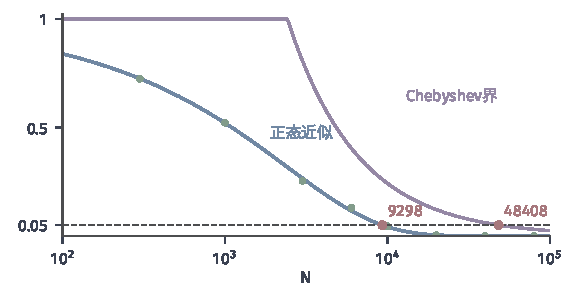
\includegraphics[width=96mm]{figures/07-probability/08-sampling-and-integration/matplotlib/mcerr-chebyshev/figure.pdf}
 \caption{$f(u)=\mathrm{e}^{u}$的样本平均误差至少为$\varepsilon=0.01$的概率。紫线为Chebyshev界$\min\{1,\sigma_f^{2}/(N\varepsilon^{2})\}$，蓝线为正态近似$2(1-\Phi(\varepsilon\sqrt{N}/\sigma_f))$，绿点为每个$N$下$2000$次重复的频率（种子$3104$）。红点标出两条曲线降到$0.05$时的样本量。}
 \label{fig:mcerr-chebyshev}
\end{BookInlineFigure}

\paragraph{二阶矩不可省}
$N^{-1/2}$的尺度完全来自方差有限。只有$\mathbb{E}_{\pi}\lvert f\rvert<\infty$时，式~\eqref{eq:mcerr-consistency}仍然成立，但误差缩小的速度可以慢得多。取$f(u)=u^{-3/4}$，$\pi=\operatorname{Unif}(0,1)$，则
\[
 I=\int_0^1u^{-3/4}\,\mathrm{d}u=4,\qquad \mathbb{E}[f(U)^{2}]=\int_0^1u^{-3/2}\,\mathrm{d}u=\infty .
\]
$f$在$0$附近趋于无穷，偶尔抽到很小的$u$，就产生一个很大的函数值。

这些大值决定了误差的尺度。$f(U)>t$当且仅当$U<t^{-4/3}$，所以
\[
 \mathbb{P}\bigl(f(U)>t\bigr)=t^{-4/3},\qquad t\geq1 .
\]
$N$个样本中至少有一个超过$t$的概率约为$Nt^{-4/3}$，它在$t\approx N^{3/4}$时变为一的量级。于是$N$个样本中最大的函数值通常在$N^{3/4}$附近，它对平均的贡献约为$N^{3/4}/N=N^{-1/4}$。每个尺度上都以不可忽略的概率出现这样的大项，平均的误差也就按$N^{-1/4}$而不是$N^{-1/2}$缩小。把这个论证写严格，需要独立和在无穷方差下的极限理论，篇幅较长，读者可查阅~\scite{math-kallenberg2021probability}。

图~\ref{fig:mcerr-heavy-paths}(a)是五次运行的运行平均：路径大部分时间偏低，每遇到一个很小的$u$就向上跳一次，然后慢慢回落。图(b)画出最大单项对平均的贡献$\max_{i\leq N}f(U_i)/N$，它沿着$N^{-1/4}$下降。图~\ref{fig:mcerr-rmse-rate}(b)用中位绝对误差衡量精度（均方误差在这里是无穷），它从$N=100$时的$0.986$降到$N=10^{5}$时的$0.172$，比值$5.73$与$1000^{1/4}=5.62$相符。按这个速度，误差缩小到十分之一要把样本数增加一万倍。

\begin{BookInlineFigure}
 \centering
 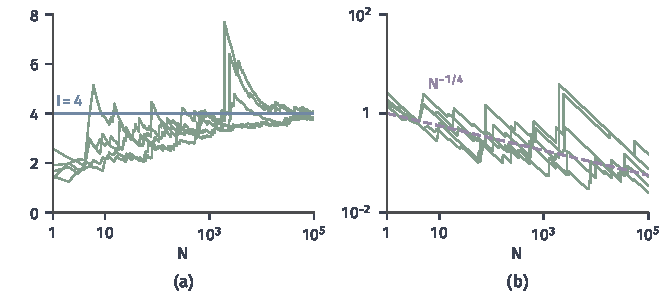
\includegraphics[width=112mm]{figures/07-probability/08-sampling-and-integration/matplotlib/mcerr-heavy-paths/figure.pdf}
 \caption{$f(u)=u^{-3/4}$的五次独立运行（种子$3105$至$3109$），横轴为对数刻度。(a)运行平均（绿线）与$I=4$（蓝线）；(b)最大单项的贡献$\max_{i\leq N}f(U_i)/N$（绿线）与参考线$N^{-1/4}$（紫色虚线），纵轴为对数刻度。}
 \label{fig:mcerr-heavy-paths}
\end{BookInlineFigure}

\begin{BookInlineFigure}
 \centering
 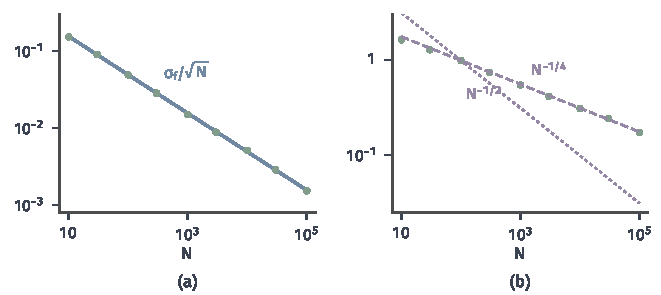
\includegraphics[width=112mm]{figures/07-probability/08-sampling-and-integration/matplotlib/mcerr-rmse-rate/figure.pdf}
 \caption{误差随样本数的变化，双对数坐标，每个$N$重复$1000$次。(a)$f(u)=\mathrm{e}^{u}$：绿点为模拟的均方根误差（种子$3102$），蓝线为$\sigma_f/\sqrt{N}$；(b)$f(u)=u^{-3/4}$：绿点为中位绝对误差（种子$3103$），紫色虚线与点线分别是斜率$-1/4$与$-1/2$的参考线。}
 \label{fig:mcerr-rmse-rate}
\end{BookInlineFigure}

\subsection{渐近误差区间}
\label{sec:mcerr-asymptotic-interval}

Chebyshev界保守，因为它只用了方差。样本数较大时，中心极限定理给出误差的近似分布，从而给出更紧的误差范围。实际计算中$\sigma_f$通常未知，要用同一批样本估计它。样本函数值的样本方差记为
\begin{equation}
 S_N^{2}=\frac{1}{N-1}\sum_{i=1}^{N}\bigl(f(X_i)-\hat{I}_N\bigr)^{2},\qquad N\geq2 .
 \label{eq:mcerr-sample-var}
\end{equation}

\begin{theorem}[独立样本的渐近误差区间]
\label{thm:mcerr-iid-clt}
设$X_1,X_2,\dots$独立且都服从$\pi$，$0<\sigma_f^{2}<\infty$。则
\begin{equation}
 \frac{\sqrt{N}\,(\hat{I}_N-I)}{S_N}\xrightarrow{\mathrm{d}}\mathcal{N}(0,1) .
 \label{eq:mcerr-studentized}
\end{equation}
因此对$0<\alpha<1$及$z=\Phi^{-1}(1-\alpha/2)$，
\begin{equation}
 \lim_{N\to\infty}\mathbb{P}\Bigl(I\in\Bigl[\hat{I}_N-\frac{zS_N}{\sqrt{N}},\ \hat{I}_N+\frac{zS_N}{\sqrt{N}}\Bigr]\Bigr)=1-\alpha .
 \label{eq:mcerr-iid-interval}
\end{equation}
\end{theorem}

\begin{proof}
$f(X_i)$独立同分布，方差为有限正数$\sigma_f^{2}$。由第~\ref{chap:central-limit-theorem}章独立同分布的中心极限定理，
\[
 \frac{\sqrt{N}\,(\hat{I}_N-I)}{\sigma_f}\xrightarrow{\mathrm{d}}\mathcal{N}(0,1) .
\]
由第~\ref{chap:laws-of-large-numbers}章样本方差的强大数律，$S_N^{2}\to\sigma_f^{2}$几乎必然成立，因而$\sigma_f/S_N\to1$依概率成立（$S_N=0$的概率趋于零，在该事件上任意规定比值即可）。式~\eqref{eq:mcerr-studentized}的左边是上式左边乘以$\sigma_f/S_N$，由第~\ref{chap:weak-convergence-of-distributions}章的Slutsky定理，乘积依分布收敛到$\mathcal{N}(0,1)$。

标准正态分布函数连续，由同一章的分布函数判据，对每个$z$，
\[
 \mathbb{P}\Bigl(\Bigl\lvert\frac{\sqrt{N}(\hat{I}_N-I)}{S_N}\Bigr\rvert\leq z\Bigr)\to\Phi(z)-\Phi(-z)=1-\alpha .
\]
左边的事件正是$I$落在式~\eqref{eq:mcerr-iid-interval}的区间中。
\end{proof}

式~\eqref{eq:mcerr-iid-interval}中的区间称为\term{渐近误差区间}（asymptotic error interval），$1-\alpha$称为名义覆盖概率；$\alpha=0.05$时$z=1.96$。区间宽度与$S_N/\sqrt{N}$成正比，后者称为估计的标准误差。它与Chebyshev界的区别在于保证的类型：Chebyshev界对每个$N$成立但偏松，渐近区间只在$N\to\infty$时给出正确的覆盖概率，对固定的$N$没有任何保证。若$\sigma_f$已知且三阶矩有限，第~\ref{chap:central-limit-theorem}章的Berry--Esseen界给出正态近似误差按$N^{-1/2}$缩小的上界；改用$S_N$以后还要加上方差估计的误差。

\paragraph{五个点的区间}
用上一节的五个均匀随机数。函数值的平均为$1.8233$，由式~\eqref{eq:mcerr-sample-var}，
\[
 S_5^{2}=0.3391,\qquad S_5=0.5823 .
\]
$\alpha=0.05$时区间半宽为
\[
 \frac{1.96\times0.5823}{\sqrt5}=0.5104 ,
\]
区间为$[1.3129,\,2.3337]$，包含$I=1.7183$。但这一次包含不说明区间可靠。图~\ref{fig:mcerr-rare-coverage}(b)的蓝线是每个$N$下$20000$次重复的实际覆盖频率：$N=5$时只有$0.868$，$N=20$时为$0.935$，$N\geq100$以后才与$0.95$相差无几。

\paragraph{稀有的大贡献}
覆盖概率接近名义值所需的样本数可以大得多。设$\pi=\operatorname{Unif}(0,1)$，
\[
 f(u)=1+1000\cdot\mathbf{1}_{\{u>0.999\}} .
\]
它有界，各阶矩都有限，定理~\ref{thm:mcerr-iid-clt}的条件全部满足。积分与方差分别是
\[
 I=1+1000\times0.001=2,\qquad \sigma_f^{2}=1000^{2}\times0.001\times0.999=999 .
\]
积分的一半来自一个概率只有千分之一的区域。

取$N=500$。一次也没有抽到$u>0.999$的概率是
\[
 0.999^{500}=\mathrm{e}^{500\ln0.999}=0.6064 .
\]
在这个事件上，所有函数值都等于$1$，于是$\hat{I}_N=1$，$S_N=0$，区间退化为单点$\{1\}$，不包含$I=2$。计算者看到的是一组完全一致的函数值和零标准误差，没有任何迹象显示有问题。

若恰好抽到一次，$\hat{I}_N=1+1000/500=3$。$499$个值与平均相差$-2$，一个值相差$998$，所以
\[
 S_N^{2}=\frac{499\times4+998^{2}}{499}=\frac{998000}{499}=2000 ,
\]
区间半宽为$1.96\sqrt{2000/500}=3.92$，区间$[-0.92,\,6.92]$包含$2$。把抽中次数服从$\operatorname{Bin}(500,0.001)$的各种情形逐一相加，$N=500$时的实际覆盖概率只有$0.393$。

图~\ref{fig:mcerr-rare-coverage}(b)的黄线是这个覆盖概率随$N$的变化，按二项分布精确求和得到。$N=10^{3}$时为$0.632$，$N=10^{4}$时才到$0.926$。图(a)是五次运行的运行平均：每条路径都先平稳地停在$1$，直到第一次抽中才突然跳起。在跳起之前，运行平均、样本方差和区间都“看起来稳定”。

即使把同一计算独立重复五次，五次都没有抽中的概率仍有$0.6064^{5}=0.082$。重复运行可以发现运行之间的分歧，但发现不了每次运行都漏掉的东西。定理~\ref{thm:mcerr-iid-clt}在这里并没有失效，它只说$N$足够大时覆盖概率接近名义值；“足够大”要比$1/0.001$大很多，而这个尺度是由$f$的结构决定的，从样本中看不出来。能防止这类错误的，是对$f$与$\pi$本身的分析，例如知道函数值的上界或贡献集中的区域，第~\ref{chap:variance-reduction}章的重要性采样正是利用这类信息。

\begin{BookInlineFigure}
 \centering
 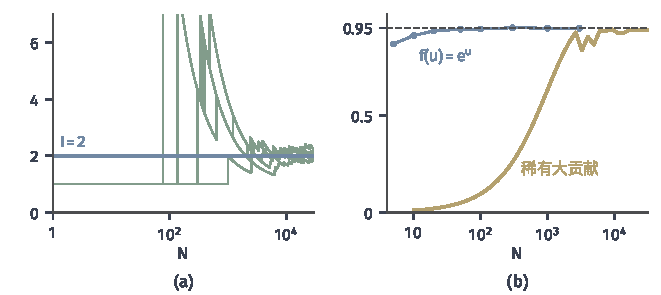
\includegraphics[width=112mm]{figures/07-probability/08-sampling-and-integration/matplotlib/mcerr-rare-coverage/figure.pdf}
 \caption{稀有大贡献$f(u)=1+1000\cdot\mathbf{1}_{\{u>0.999\}}$，$I=2$。(a)五次独立运行的运行平均（绿线，种子$3110$至$3114$）与$I$（蓝线），横轴为对数刻度；(b)渐近区间$\hat{I}_N\pm1.96S_N/\sqrt{N}$的实际覆盖概率：黄线为稀有大贡献的精确值，蓝线为$f(u)=\mathrm{e}^{u}$在每个$N$下$20000$次重复的频率（种子$3115$），虚线为名义值$0.95$。}
 \label{fig:mcerr-rare-coverage}
\end{BookInlineFigure}


\section{近似生成的偏差}
\label{sec:mcerr-approx}

实际程序很少精确地服从$\pi$。分位数没有解析式时要数值反演，连续时间的动态要离散化，有时还会像上一节的例子那样为了数值安全截断输出。设程序独立地产生服从$\tilde{\pi}$的样本，$\tilde{\pi}$与$\pi$接近但不相等。对在两种分布下都可积的$f$，记
\begin{equation}
 b=\mathbb{E}_{\tilde{\pi}}[f]-\mathbb{E}_{\pi}[f] .
 \label{eq:mcerr-approx-bias}
\end{equation}
这是由生成规律本身带来的积分偏差，与样本数无关。

\paragraph{偏差不随样本数消失}
样本独立且都服从$\tilde{\pi}$，第~\ref{sec:mcerr-iid}节的结论对$\tilde{\pi}$成立：$\hat{I}_N$几乎必然收敛到$\mathbb{E}_{\tilde{\pi}}[f]=I+b$，而不是$I$。若$\mathbb{E}_{\tilde{\pi}}[f^{2}]<\infty$，由定理~\ref{thm:mcerr-mse}，
\begin{equation}
 \mathbb{E}\bigl[(\hat{I}_N-I)^{2}\bigr]=b^{2}+\frac{\operatorname{Var}_{\tilde{\pi}}(f)}{N}\geq b^{2} .
 \label{eq:mcerr-approx-mse}
\end{equation}
增加同一近似方法的样本数只能压低第二项，均方误差最终停在$b^{2}$。

回到截断程序$\tilde{X}=\min\{X,2\}$。它的二阶矩可以由尾概率算出：
\[
 \mathbb{E}[\min\{X,T\}^{2}]=\int_0^{T}2t\,\mathrm{e}^{-t}\,\mathrm{d}t=2\bigl(1-(1+T)\mathrm{e}^{-T}\bigr) .
\]
$T=2$时它等于$1.1880$，减去均值的平方$0.8647^{2}=0.7476$，得到
\[
 \operatorname{Var}_{\tilde{\pi}}(f)=0.4403,\qquad b^{2}=\mathrm{e}^{-4}=0.0183 .
\]
两项在$N=0.4403/0.0183\approx24$时相等。样本数超过几十以后，误差几乎全由偏差决定。

图~\ref{fig:mcerr-approx-bias}(a)中五条运行平均都收敛到$1-\mathrm{e}^{-2}$，离$I=1$始终差$0.135$。图(b)比较两个程序的均方根误差：精确程序沿$1/\sqrt{N}$一直下降，截断程序在$N$超过几十后变平，停在$\lvert b\rvert$。这时只看运行平均是否稳定、标准误差是否很小，会得到一个精确地错了的答案。

\begin{BookInlineFigure}
 \centering
 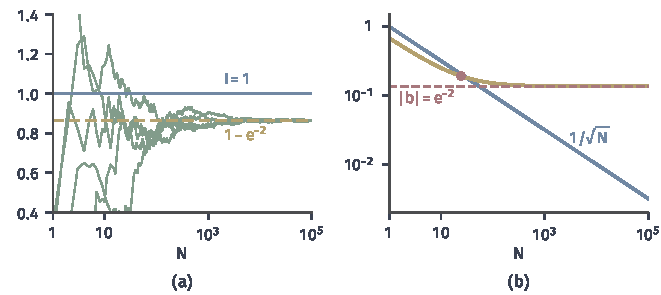
\includegraphics[width=112mm]{figures/07-probability/08-sampling-and-integration/matplotlib/mcerr-approx-bias/figure.pdf}
 \caption{截断程序$\min\{X,2\}$估计$\mathbb{E}[X]=1$，$X\sim\operatorname{Exp}(1)$，横轴为对数刻度。(a)五次运行的运行平均（绿线，种子$3116$至$3120$），蓝线为$I=1$，黄色虚线为$\tilde{\pi}$下的均值$1-\mathrm{e}^{-2}$；(b)均方根误差的精确值：蓝线为精确程序的$1/\sqrt{N}$，黄线为截断程序的$\sqrt{b^{2}+0.4403/N}$，红色虚线为$\lvert b\rvert=\mathrm{e}^{-2}$，红点标出方差项等于$b^{2}$的$N\approx24$。}
 \label{fig:mcerr-approx-bias}
\end{BookInlineFigure}

\paragraph{有界被积函数}
偏差无法从样本中读出，只能从$\tilde{\pi}$与$\pi$的差别估计出来。第~\ref{chap:distribution-comparison}章的总变差正好衡量这种差别：对有界的$f$，记$\operatorname{osc}(f)=\sup f-\inf f$，那里证明了
\begin{equation}
 \lvert b\rvert=\bigl\lvert\mathbb{E}_{\tilde{\pi}}[f]-\mathbb{E}_{\pi}[f]\bigr\rvert\leq\operatorname{osc}(f)\,d_{\mathrm{TV}}(\tilde{\pi},\pi)\leq2\sup\lvert f\rvert\,d_{\mathrm{TV}}(\tilde{\pi},\pi) .
 \label{eq:mcerr-tv-bound}
\end{equation}
所以只要知道近似分布与目标的总变差，就同时控制了所有有界被积函数的偏差。

截断程序的总变差可以直接算出。$\tilde{\pi}$在$[0,2)$上与$\pi$有相同的密度，把$\pi$在$(2,\infty)$上的质量$\mathrm{e}^{-2}$全部堆到点$2$上，如图~\ref{fig:mcerr-tv-bias}(a)。对任一事件$A$，差别只来自$A$与$\{2\}$、$(2,\infty)$的交，所以
\[
 \lvert\tilde{\pi}(A)-\pi(A)\rvert\leq\mathrm{e}^{-2},
\]
取$A=(2,\infty)$时等号成立，所以
\[
 d_{\mathrm{TV}}(\tilde{\pi},\pi)=\mathrm{e}^{-2} .
\]
对$f=\mathbf{1}_{\{x>2\}}$，$\operatorname{osc}(f)=1$，偏差恰为$-\mathrm{e}^{-2}$，式~\eqref{eq:mcerr-tv-bound}取到等号；对$f=\mathbf{1}_{\{x>1\}}$，截断不改变事件$\{X>1\}$，偏差为零。

\paragraph{无界被积函数}
对无界的$f$，总变差小并不能保证偏差小。设$\varepsilon\in(0,1)$，$c>1$，令近似分布为
\[
 \tilde{\pi}_{\varepsilon}=(1-\varepsilon)\,\pi+\varepsilon\,\delta_{c},\qquad \pi=\operatorname{Exp}(1) ,
\]
即以概率$1-\varepsilon$正常生成，以概率$\varepsilon$输出一个远处的值$c$。对任一事件$A$，
\[
 \lvert\tilde{\pi}_{\varepsilon}(A)-\pi(A)\rvert=\varepsilon\,\lvert\delta_{c}(A)-\pi(A)\rvert\leq\varepsilon ,
\]
所以$d_{\mathrm{TV}}\leq\varepsilon$。对$f(x)=x$，偏差却是$\varepsilon(c-1)$。取$c=1/\varepsilon^{2}$，总变差趋于零时偏差$1/\varepsilon-\varepsilon$趋于无穷。

图~\ref{fig:mcerr-tv-bias}(b)对照了这两种情形：有界的$f$的偏差随$\varepsilon$线性缩小，$f(x)=x$的偏差反而增大。问题出在少量质量被放到了很远的地方。总变差只问“同一事件的概率差多少”，不问质量移到了哪里；无界函数却对远处的质量非常敏感。

\begin{BookInlineFigure}
 \centering
 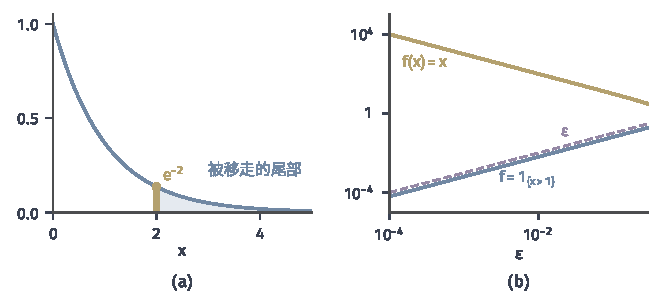
\includegraphics[width=112mm]{figures/07-probability/08-sampling-and-integration/matplotlib/mcerr-tv-bias/figure.pdf}
 \caption{总变差与积分偏差。(a)$\operatorname{Exp}(1)$的密度（蓝线）；截断程序把浅蓝区域中的尾部质量移到点$2$，形成质量为$\mathrm{e}^{-2}$的原子（黄色竖线，高度表示质量）。(b)近似分布$(1-\varepsilon)\operatorname{Exp}(1)+\varepsilon\delta_{1/\varepsilon^{2}}$的总变差不超过$\varepsilon$（紫色虚线）；蓝线为$f=\mathbf{1}_{\{x>1\}}$的偏差$\varepsilon(1-\mathrm{e}^{-1})$，黄线为$f(x)=x$的偏差$1/\varepsilon-\varepsilon$，双对数坐标。}
 \label{fig:mcerr-tv-bias}
\end{BookInlineFigure}

要让总变差重新起作用，需要控制两种分布在远处的质量。下面用二阶矩给出一个简单的结论。

\begin{lemma}[矩控制下的偏差界]
\label{lem:mcerr-moment-tv}
设$\mathbb{E}_{\pi}[f^{2}]\leq m$，$\mathbb{E}_{\tilde{\pi}}[f^{2}]\leq m$，记$d=d_{\mathrm{TV}}(\tilde{\pi},\pi)$。则
\begin{equation}
 \bigl\lvert\mathbb{E}_{\tilde{\pi}}[f]-\mathbb{E}_{\pi}[f]\bigr\rvert\leq4\sqrt{m\,d} .
 \label{eq:mcerr-moment-tv}
\end{equation}
\end{lemma}

\begin{proof}
$d=0$时两分布相同，结论成立。设$d>0$，固定截断水平$t>0$，把$f$分成有界部分与尾部：
\[
 f=f\,\mathbf{1}_{\{\lvert f\rvert\leq t\}}+f\,\mathbf{1}_{\{\lvert f\rvert>t\}} .
\]
有界部分的振幅不超过$2t$，由式~\eqref{eq:mcerr-tv-bound}，它在两分布下的期望差不超过$2td$。

尾部在$\lvert f\rvert>t$时满足$\lvert f\rvert\leq f^{2}/t$，所以对$\pi$与$\tilde{\pi}$都有
\[
 \bigl\lvert\mathbb{E}\bigl[f\,\mathbf{1}_{\{\lvert f\rvert>t\}}\bigr]\bigr\rvert\leq\frac{\mathbb{E}[f^{2}]}{t}\leq\frac{m}{t} .
\]
两分布下的尾部期望之差不超过$2m/t$。合起来，偏差不超过$2td+2m/t$。取$t=\sqrt{m/d}$，两项都等于$2\sqrt{md}$。
\end{proof}

证明里的截断水平体现了两种误差的折中：$t$越大，有界部分越宽，总变差的作用被放大；$t$越小，留在尾部的质量越多。界$4\sqrt{md}$随$d$按平方根缩小，比有界情形的线性缩小慢，这是为控制尾部付出的代价。对截断程序，$f(x)=x$在两分布下的二阶矩分别是$2$和$1.188$，取$m=2$，界为
\[
 4\sqrt{2\times0.1353}=2.081 ,
\]
远大于实际的$0.1353$，但它不依赖任何具体计算。对$\tilde{\pi}_{\varepsilon}$，二阶矩至少为$\varepsilon c^{2}=\varepsilon^{-3}$，代入后界的量级是$4/\varepsilon$，与实际偏差的量级一致：矩条件正好抓住了远处质量的作用。

\paragraph{近似转移}
用Markov链采样时，近似发生在转移这一步：理论上的转移核$K$以$\pi$为不变分布，实际程序执行的却是另一个核$\tilde{K}$。这时要先回答一个更基本的问题：$\tilde{K}$有没有不变分布，有的话它离$\pi$多远。链跑得再久，平均也只能趋向$\tilde{K}$自己的长期规律。

看一个可以算到底的例子。目标是$\pi=\mathcal{N}(0,1)$，某个由连续时间动态离散化得到的更新为
\[
 X^{(t+1)}=(1-h)X^{(t)}+\sqrt{2h}\,\xi^{(t+1)} ,
\]
其中$\xi^{(1)},\xi^{(2)},\dots$独立且服从$\mathcal{N}(0,1)$，与$X^{(0)}$独立，$h>0$是步长。若$X^{(t)}\sim\mathcal{N}(0,v)$，则$X^{(t+1)}\sim\mathcal{N}(0,(1-h)^{2}v+2h)$。令两者相等，
\[
 v=(1-h)^{2}v+2h,\qquad v=\frac{2h}{1-(1-h)^{2}}=\frac{2}{2-h},\qquad 0<h<2 .
\]
所以$0<h<2$时，$\mathcal{N}(0,2/(2-h))$是这个近似转移的不变分布，而$\pi$不是。

从任意$x$出发，展开递推得到
\[
 X^{(t)}=(1-h)^{t}x+\sum_{j=1}^{t}(1-h)^{t-j}\sqrt{2h}\,\xi^{(j)} ,
\]
它服从均值为$(1-h)^{t}x$、方差为$2h\sum_{j<t}(1-h)^{2j}$的高斯分布。$\lvert1-h\rvert<1$时，均值趋于零，方差趋于$v$，链确实趋向这个不变分布。取$h=0.5$，$v=4/3$。对$f(x)=x^{2}$，偏差为$4/3-1=1/3$；对有界的$f=\mathbf{1}_{\{\lvert x\rvert\leq1\}}$，
\[
 \mathbb{P}_{\mathcal{N}(0,4/3)}\bigl(\lvert X\rvert\leq1\bigr)=2\Phi\bigl(\sqrt{3}/2\bigr)-1=0.6135 ,
\]
而目标值是$2\Phi(1)-1=0.6827$，偏差为$-0.0692$。图~\ref{fig:mcerr-approx-chain}(b)中，$10^{5}$步的直方图贴合的是$\mathcal{N}(0,4/3)$，不是$\pi$。

$h\geq2$时，不变分布根本不存在。设$\mu$是不变分布，$\phi$是它的特征函数，则$X\sim\mu$与独立的$\xi$满足$(1-h)X+\sqrt{2h}\,\xi\sim\mu$，即
\[
 \phi(s)=\phi\bigl((1-h)s\bigr)\,\mathrm{e}^{-hs^{2}} .
\]
记$c=\lvert1-h\rvert\geq1$。特征函数的模不超过$1$，把上式反复代入$k$次，
\[
 \lvert\phi(s)\rvert\leq\exp\Bigl(-hs^{2}\sum_{j=0}^{k-1}c^{2j}\Bigr)\leq\mathrm{e}^{-khs^{2}} .
\]
令$k\to\infty$，对每个$s\neq0$得$\phi(s)=0$。这与特征函数在$0$处连续且$\phi(0)=1$矛盾。图~\ref{fig:mcerr-approx-chain}(a)画出不变方差$2/(2-h)$，它在$h\to2$时趋于无穷。

\begin{BookInlineFigure}
 \centering
 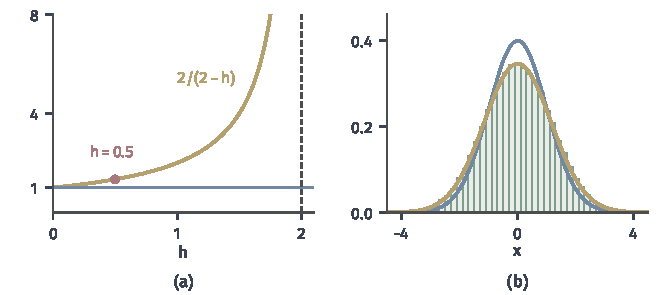
\includegraphics[width=112mm]{figures/07-probability/08-sampling-and-integration/matplotlib/mcerr-approx-chain/figure.pdf}
 \caption{近似转移$X'=(1-h)X+\sqrt{2h}\,\xi$，目标为$\mathcal{N}(0,1)$。(a)不变分布的方差$2/(2-h)$（黄线）与目标方差$1$（蓝线），灰色虚线为$h=2$，红点为$h=0.5$；(b)$h=0.5$时从$0$出发运行$10^{5}$步的直方图（绿色，种子$3121$），蓝线为目标密度，黄线为不变分布$\mathcal{N}(0,4/3)$的密度。}
 \label{fig:mcerr-approx-chain}
\end{BookInlineFigure}

这个例子显示了近似链需要分两步检查。先确认近似转移存在不变分布、并且链会趋向它；再估计它与$\pi$的差，必要时减小步长或用第~\ref{chap:sample-generation}章的Metropolis接受步骤校正，使$\pi$恢复为精确的不变分布。两步都与运行长度无关。


\section{链初值的影响}
\label{sec:mcerr-initial}

现在设转移是精确的。第~\ref{chap:sample-generation}章用转移核$K(x,A)$描述链：当前状态为$x$时，下一状态落入$A$的概率为$K(x,A)$。若
\[
 \int_{\mathcal{X}}K(x,A)\,\pi(\mathrm{d}x)=\pi(A)\qquad\text{对每个事件}A ,
\]
就称$\pi$是不变分布。链从$X^{(0)}$出发，依次生成$X^{(1)},X^{(2)},\dots$，用
\begin{equation}
 \hat{I}_N=\frac1N\sum_{t=1}^{N}f\bigl(X^{(t)}\bigr)
 \label{eq:mcerr-chain-average}
\end{equation}
估计$I$。这一节研究链从哪里出发怎样影响这个平均的偏差。

\paragraph{从目标分布出发}
若$X^{(0)}\sim\pi$，由不变性，$X^{(1)}$的分布是
\[
 \mathbb{P}(X^{(1)}\in A)=\int K(x,A)\,\pi(\mathrm{d}x)=\pi(A) ,
\]
依次类推，每个$X^{(t)}$都服从$\pi$。由第~\ref{sec:mcerr-estimator}节，偏差只看各项的分布，所以$\hat{I}_N$无偏，尽管各项高度相关。这样的链称为平稳的：任意时刻的状态都服从$\pi$。

\paragraph{从一般初值出发}
实际中能精确从$\pi$出发，往往就不需要链了。设$X^{(0)}\sim\mu$。记$K^{t}(x,\cdot)$为从$x$出发$t$步后状态的分布，则$X^{(t)}$的分布是$\mu K^{t}=\int\mu(\mathrm{d}x)\,K^{t}(x,\cdot)$，一般不等于$\pi$。设各项可积，偏差为
\begin{equation}
 b_N=\frac1N\sum_{t=1}^{N}\Bigl(\mathbb{E}_{\mu K^{t}}[f]-I\Bigr) .
 \label{eq:mcerr-initial-bias}
\end{equation}
偏差的大小取决于边缘分布$\mu K^{t}$趋近$\pi$的快慢。

\paragraph{一条可以算到底的链}
下面这条链贯穿本章后半部分。取$\pi=\mathcal{N}(0,1)$，$\lvert\rho\rvert<1$，令
\begin{equation}
 X^{(t+1)}=\rho X^{(t)}+\sqrt{1-\rho^{2}}\,\xi^{(t+1)} ,
 \label{eq:mcerr-ar1}
\end{equation}
其中$\xi^{(t)}$独立且服从$\mathcal{N}(0,1)$，与$X^{(0)}$独立。若$X^{(t)}\sim\mathcal{N}(0,1)$，则$X^{(t+1)}$服从均值为$0$、方差为$\rho^{2}+(1-\rho^{2})=1$的高斯分布，所以$\pi$是不变分布。$\rho$越接近$1$，每步保留的旧状态越多，链移动越慢。

从$X^{(0)}=x_0$出发，展开递推，
\[
 X^{(t)}=\rho^{t}x_0+\sqrt{1-\rho^{2}}\sum_{j=1}^{t}\rho^{t-j}\xi^{(j)} .
\]
后一项是独立高斯变量的线性组合，方差为$(1-\rho^{2})\sum_{j=0}^{t-1}\rho^{2j}=1-\rho^{2t}$，所以
\begin{equation}
 K^{t}(x_0,\cdot)=\mathcal{N}\bigl(\rho^{t}x_0,\ 1-\rho^{2t}\bigr) .
 \label{eq:mcerr-ar1-marginal}
\end{equation}
均值以几何速度$\rho^{t}$忘掉初值。对$f(x)=x$，$I=0$，由式~\eqref{eq:mcerr-initial-bias}，偏差为几何级数之和：
\[
 b_N=\frac{x_0}{N}\sum_{t=1}^{N}\rho^{t}=\frac{x_0\,\rho\,(1-\rho^{N})}{N(1-\rho)} .
\]

取$\rho=0.9$，$x_0=10$。偏差约为$90/N$：
\[
 b_{100}=0.900,\qquad b_{1000}=0.0900 .
\]
第~\ref{sec:mcerr-long-run}小节会算出平稳时这条链平均的标准差约为$\sqrt{19/N}$，$N=100$时为$0.436$，比偏差还小。偏差按$1/N$缩小，标准差按$1/\sqrt{N}$缩小，所以记录足够长时初值的影响终将被波动淹没，但在中等长度上它可以是误差的主要部分。图~\ref{fig:mcerr-burnin}(a)是$20$条从$10$出发的路径，它们沿着$0.9^{t}\times10$向$0$靠拢，大约$40$步以后才混入平稳的波动带。

\paragraph{舍弃初始一段}
常用的办法是先运行$b$步不记录，再平均接下来的$N$个状态，被舍弃的这一段称为\term{预烧期}（burn-in period）。对上面的链，平均$X^{(b+1)},\dots,X^{(b+N)}$的偏差是
\[
 \frac{x_0\,\rho^{b+1}(1-\rho^{N})}{N(1-\rho)} .
\]
$N=100$时，$b=20$把偏差从$0.900$降到$0.109$，$b=50$降到$0.0046$，如图~\ref{fig:mcerr-burnin}(b)。

\begin{BookInlineFigure}
 \centering
 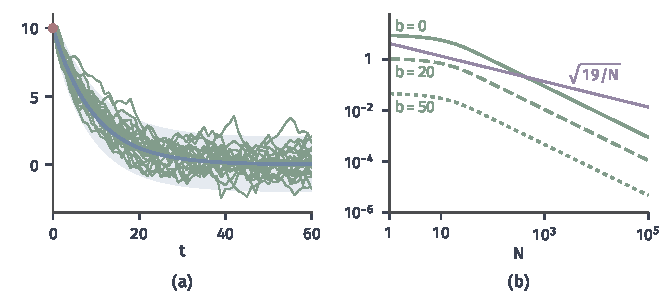
\includegraphics[width=112mm]{figures/07-probability/08-sampling-and-integration/matplotlib/mcerr-burnin/figure.pdf}
 \caption{链~\eqref{eq:mcerr-ar1}在$\rho=0.9$时从$x_0=10$（红点）出发。(a)$20$条路径（绿线，种子$3122$），蓝线为边缘均值$0.9^{t}x_0$，浅蓝带为边缘均值加减两倍边缘标准差；(b)舍弃前$b$步后平均$N$步的偏差精确值（绿色实线、虚线、点线分别为$b=0,20,50$），紫线为平稳时的标准差$\sqrt{19/N}$，双对数坐标。}
 \label{fig:mcerr-burnin}
\end{BookInlineFigure}

预烧期之所以有效，是因为这里知道边缘分布以$\rho^{t}$的速度靠近$\pi$。一般地，若对有界的$f$已知$d_{\mathrm{TV}}(\mu K^{t},\pi)\leq Cr^{t}$，$0<r<1$，由式~\eqref{eq:mcerr-tv-bound}与式~\eqref{eq:mcerr-initial-bias}，舍弃$b$步后
\begin{equation}
 \lvert b_N\rvert\leq\frac{\operatorname{osc}(f)}{N}\sum_{t=b+1}^{b+N}Cr^{t}\leq\frac{\operatorname{osc}(f)\,C\,r^{b+1}}{N(1-r)} .
 \label{eq:mcerr-burnin-bound}
\end{equation}
没有这类收敛控制，预烧期就没有依据。最极端的例子是始终停在原地的转移$K(x,\cdot)=\delta_{x}$：每个分布都是它的不变分布，但从$x_0$出发的链永远停在$x_0$，舍弃多少步都不改变$\hat{I}_N=f(x_0)$。第~\ref{sec:mcerr-diagnostics}小节还会看到更隐蔽的情形：链在一个局部区域内看起来已经平稳，却始终没有到达目标的另一部分。

即使有收敛控制，舍弃之后剩下的样本也不是精确平稳的。在式~\eqref{eq:mcerr-ar1-marginal}中，任何有限的$t$都有$1-\rho^{2t}<1$，$K^{t}(x_0,\cdot)$从来不等于$\pi$。预烧期只是把偏差压到可以忽略的量级，这个量级需要由式~\eqref{eq:mcerr-burnin-bound}这样的估计给出。

\paragraph{无界被积函数}
式~\eqref{eq:mcerr-burnin-bound}要求$f$有界。对无界的$f$，即使$\mu K^{t}$收敛到$\pi$，期望也未必收敛。第~\ref{chap:random-variable-convergence}章与第~\ref{chap:weak-convergence-of-distributions}章说明，分布收敛之外还需要$f(X^{(t)})$一致可积，才能保证$\mathbb{E}[f(X^{(t)})]\to\mathbb{E}_{\pi}[f]$。

仍用链~\eqref{eq:mcerr-ar1}，但让$X^{(0)}$服从二阶矩无穷的分布，例如标准Cauchy分布，取$f(x)=x^{2}$。$X^{(t)}=\rho^{t}X^{(0)}+G_t$，其中$G_t$是与$X^{(0)}$独立的高斯变量。给定$G_t$时，$\rho^{t}X^{(0)}+G_t$的二阶矩为无穷，所以对每个$t$，
\[
 \mathbb{E}\bigl[(X^{(t)})^{2}\bigr]=\infty .
\]
另一方面，$\rho^{t}X^{(0)}\to0$依概率成立，由Slutsky定理，$X^{(t)}$依分布收敛到$\mathcal{N}(0,1)$。于是对每个$N$和每个预烧期长度，$\mathbb{E}[\hat{I}_N]=\infty$，偏差没有意义，舍弃初始段也无济于事。初值的尾部经过任意有限步都没有被完全忘掉，正是这种残留破坏了一致可积性。


\section{相关平均的方差}
\label{sec:mcerr-correlated}

上一节处理的是链平均的偏差，现在把它放在一边，假定链从$\pi$出发，于是$\hat{I}_N$无偏，误差只剩随机波动。链的相邻状态相关，式~\eqref{eq:mcerr-iid-var}的推导用到了独立性，不能照搬。相关性究竟让波动变大还是变小，变多少？先对固定的$N$精确计算方差，再看$N$很大时它的主要部分。

\subsection{平稳平均的方差}
\label{sec:mcerr-stationary-var}

设链平稳，$\mathbb{E}_{\pi}[f^{2}]<\infty$。对任意时刻$s$，$X^{(s)}\sim\pi$，并且从$X^{(s)}$往后按同一个核演化，所以$(X^{(s)},X^{(s+k)})$与$(X^{(0)},X^{(k)})$有相同的联合分布。于是两时刻函数值的协方差只依赖时间差$k$，记
\begin{equation}
 \gamma_k=\operatorname{Cov}_{\pi}\bigl(f(X^{(0)}),f(X^{(k)})\bigr),\qquad k=0,1,2,\dots
 \label{eq:mcerr-autocov}
\end{equation}
它称为$f$沿链的\term{自协方差}（autocovariance）。$\gamma_0=\operatorname{Var}_{\pi}(f)$，由Cauchy--Schwarz不等式，$\lvert\gamma_k\rvert\leq\gamma_0$。

\begin{theorem}[平稳平均的方差]
\label{thm:mcerr-stationary-var}
设链平稳，$\mathbb{E}_{\pi}[f^{2}]<\infty$。则对每个$N\geq1$，
\begin{equation}
 \operatorname{Var}(\hat{I}_N)=\frac1N\Bigl[\gamma_0+2\sum_{k=1}^{N-1}\Bigl(1-\frac{k}{N}\Bigr)\gamma_k\Bigr] .
 \label{eq:mcerr-stationary-var}
\end{equation}
\end{theorem}

\begin{proof}
记$Y_t=f(X^{(t)})$。和的方差等于全部协方差之和，
\[
 \operatorname{Var}\Bigl(\sum_{t=1}^{N}Y_t\Bigr)=\sum_{s=1}^{N}\sum_{t=1}^{N}\operatorname{Cov}(Y_s,Y_t)=\sum_{s=1}^{N}\sum_{t=1}^{N}\gamma_{\lvert s-t\rvert} .
\]
在$N\times N$的下标方阵中，$\lvert s-t\rvert=0$的格子有$N$个（对角线）；对$1\leq k\leq N-1$，$\lvert s-t\rvert=k$的格子在对角线两侧各有$N-k$个。按$k$合并，
\[
 \operatorname{Var}\Bigl(\sum_{t=1}^{N}Y_t\Bigr)=N\gamma_0+2\sum_{k=1}^{N-1}(N-k)\gamma_k .
\]
两边除以$N^{2}$即得。
\end{proof}

与独立情形比较，式~\eqref{eq:mcerr-stationary-var}多了方括号里的求和。各$\gamma_k$为正时，方差大于$\gamma_0/N$：相邻状态差不多，第二个样本带来的新信息少于一个独立样本，好比反复询问同一户人家。各$\gamma_k$正负交替时，方差可以小于$\gamma_0/N$：相邻状态落在两侧，平均时互相抵消。所以链输出的方差既可能比独立平均大，也可能比它小；直接把$S_N^{2}/N$当作链平均的方差，没有任何依据。

\paragraph{例子中的自协方差}
对链~\eqref{eq:mcerr-ar1}与$f(x)=x$，$X^{(k)}$等于$\rho^{k}X^{(0)}$加上一个与$X^{(0)}$独立的项，所以
\[
 \gamma_k=\operatorname{Cov}\bigl(X^{(0)},\rho^{k}X^{(0)}\bigr)=\rho^{k} .
\]
对$f(x)=x^{2}$，记$Z$为与$X^{(0)}$独立的标准正态变量，$X^{(k)}=\rho^{k}X^{(0)}+\sqrt{1-\rho^{2k}}\,Z$，平方后
\[
 (X^{(k)})^{2}=\rho^{2k}(X^{(0)})^{2}+2\rho^{k}\sqrt{1-\rho^{2k}}\,X^{(0)}Z+(1-\rho^{2k})Z^{2} .
\]
与$(X^{(0)})^{2}$求协方差时，第二项的协方差是$\mathbb{E}[(X^{(0)})^{3}]\,\mathbb{E}[Z]=0$，第三项与$X^{(0)}$独立，只剩第一项。标准正态变量平方的方差是$2$，所以$\gamma_k=2\rho^{2k}$。

\paragraph{四步的平均}
取$N=4$，$f(x)=x$。$\rho=0.9$时，由式~\eqref{eq:mcerr-stationary-var}，
\[
 \operatorname{Var}(\hat{I}_4)=\frac14\bigl[1+2(0.75\times0.9+0.5\times0.81+0.25\times0.729)\bigr]=\frac{3.5245}{4}=0.8811 .
\]
$\rho=-0.5$时，
\[
 \operatorname{Var}(\hat{I}_4)=\frac14\bigl[1+2(-0.75\times0.5+0.5\times0.25-0.25\times0.125)\bigr]=\frac{0.4375}{4}=0.1094 .
\]
同样长度的独立平均方差是$0.25$。正相关的链把方差放大到约$3.5$倍，负相关的链把它缩小到约$0.44$倍。

图~\ref{fig:mcerr-ar-paths}用同一串噪声画出三条平稳链。$\rho=0.9$的路径缓慢起伏，$80$步的平均为$0.45$；$\rho=0$即独立样本，平均为$0.097$；$\rho=-0.5$的路径在$0$两侧来回跳，平均只有$0.055$。图~\ref{fig:mcerr-autocov}(a)画出两种$\rho$下的$\gamma_k$。

\begin{BookInlineFigure}
 \centering
 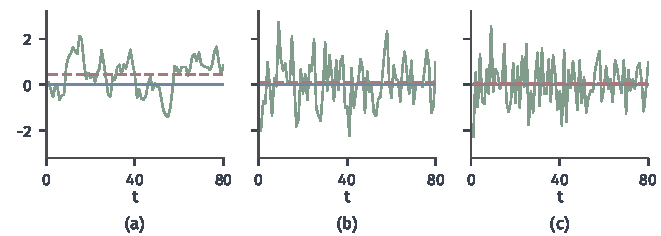
\includegraphics[width=112mm]{figures/07-probability/08-sampling-and-integration/matplotlib/mcerr-ar-paths/figure.pdf}
 \caption{平稳链~\eqref{eq:mcerr-ar1}的$80$步路径（绿线），三图使用同一串噪声与初值（种子$3129$）。(a)$\rho=0.9$；(b)$\rho=0$；(c)$\rho=-0.5$。蓝线为$I=0$，红色虚线为$80$步的平均。}
 \label{fig:mcerr-ar-paths}
\end{BookInlineFigure}

\subsection{长期方差}
\label{sec:mcerr-long-run}

链平均的方差公式~\eqref{eq:mcerr-stationary-var}含有$N$个项，比较两条链或两个被积函数时不方便。$N$很大时，权重$1-k/N$对固定的$k$趋于$1$，方括号趋于一个与$N$无关的数，它就是比较精度时需要的量。

\begin{definition}[长期方差]
\label{def:mcerr-long-run}
设链平稳，$\mathbb{E}_{\pi}[f^{2}]<\infty$，且$\sum_{k\geq1}\lvert\gamma_k\rvert<\infty$。称
\begin{equation}
 \sigma_{\mathrm{LR}}^{2}=\gamma_0+2\sum_{k=1}^{\infty}\gamma_k
 \label{eq:mcerr-long-run}
\end{equation}
为$f$沿链的\term{长期方差}（long-run variance）。
\end{definition}

\begin{theorem}[方差的极限]
\label{thm:mcerr-long-run-limit}
在定义~\ref{def:mcerr-long-run}的条件下，
\begin{equation}
 \lim_{N\to\infty}N\operatorname{Var}(\hat{I}_N)=\sigma_{\mathrm{LR}}^{2} .
 \label{eq:mcerr-nvar-limit}
\end{equation}
\end{theorem}

\begin{proof}
由式~\eqref{eq:mcerr-stationary-var}与式~\eqref{eq:mcerr-long-run}，
\[
 N\operatorname{Var}(\hat{I}_N)-\sigma_{\mathrm{LR}}^{2}=-2\sum_{k=N}^{\infty}\gamma_k-2\sum_{k=1}^{N-1}\frac{k}{N}\gamma_k .
\]
第一项是收敛级数的尾部，趋于零。第二项中第$k$项$(k/N)\gamma_k\mathbf{1}_{\{k<N\}}$的绝对值不超过$\lvert\gamma_k\rvert$，而且对固定的$k$，它随$N\to\infty$趋于零。$\lvert\gamma_k\rvert$可和，由支配收敛定理（用于计数测度上的级数），第二项也趋于零。
\end{proof}

于是$N$大时$\operatorname{Var}(\hat{I}_N)\approx\sigma_{\mathrm{LR}}^{2}/N$，链平均仍按$N^{-1/2}$收缩，只是把独立情形的$\gamma_0$换成了$\sigma_{\mathrm{LR}}^{2}$。对链~\eqref{eq:mcerr-ar1}与$f(x)=x$，
\[
 \sigma_{\mathrm{LR}}^{2}=1+2\sum_{k=1}^{\infty}\rho^{k}=1+\frac{2\rho}{1-\rho}=\frac{1+\rho}{1-\rho} .
\]
$\rho=0.9$时为$19$，$\rho=-0.5$时为$1/3$。图~\ref{fig:mcerr-autocov}(b)画出$N\operatorname{Var}(\hat{I}_N)$的精确值：$\rho=0.9$时，$N=4$为$3.52$，$N=100$为$17.20$，$N=1000$为$18.82$，逐步接近$19$。接近的快慢由$\gamma_k$衰减的快慢决定。

\begin{BookInlineFigure}
 \centering
 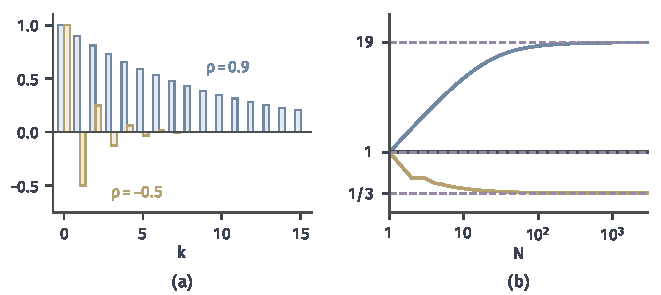
\includegraphics[width=112mm]{figures/07-probability/08-sampling-and-integration/matplotlib/mcerr-autocov/figure.pdf}
 \caption{平稳链~\eqref{eq:mcerr-ar1}与$f(x)=x$。(a)自协方差$\gamma_k=\rho^{k}$，蓝色为$\rho=0.9$，黄色为$\rho=-0.5$；(b)由式~\eqref{eq:mcerr-stationary-var}算出的$N\operatorname{Var}(\hat{I}_N)$，蓝、灰、黄线分别对应$\rho=0.9,0,-0.5$，紫色虚线为长期方差$19,1,1/3$，双对数坐标。}
 \label{fig:mcerr-autocov}
\end{BookInlineFigure}

\paragraph{可和条件不成立时}
协方差不可和时，方差的极限可以不存在。考虑状态空间$\{0,1\}$上始终停在原地的链，从$\pi=(1/2,1/2)$出发，取$f$为状态$1$的示性函数。每一步的状态都等于$X^{(0)}$，所以$\gamma_k=1/4$对所有$k$成立，级数发散；实际上$\hat{I}_N=f(X^{(0)})$，$\operatorname{Var}(\hat{I}_N)=1/4$根本不随$N$缩小，$N\operatorname{Var}(\hat{I}_N)\to\infty$。

\paragraph{方差极限不是正态极限}
定理~\ref{thm:mcerr-long-run-limit}只说明了二阶矩的尺度，没有说$\sqrt{N}(\hat{I}_N-I)$的分布趋于正态。独立情形下这一步由中心极限定理完成，链的情形还需要关于链与$f$的附加条件，第~\ref{sec:mcerr-chain-clt}小节会给出一个满足可和条件、极限却不是正态的例子。

\subsection{有效样本量}
\label{sec:mcerr-ess}

长期方差告诉我们链平均的方差约为$\sigma_{\mathrm{LR}}^{2}/N$。把它与同样被积函数的独立平均$\gamma_0/N$比较，可以换算成“相当于多少个独立样本”。

\begin{definition}[有效样本量]
\label{def:mcerr-ess}
在定义~\ref{def:mcerr-long-run}的条件下，设$0<\gamma_0<\infty$，$0<\sigma_{\mathrm{LR}}^{2}<\infty$。长度为$N$的平稳链平均的\term{有效样本量}（effective sample size）为
\begin{equation}
 N_{\mathrm{eff}}=\frac{N\gamma_0}{\sigma_{\mathrm{LR}}^{2}} .
 \label{eq:mcerr-ess}
\end{equation}
\end{definition}

由式~\eqref{eq:mcerr-nvar-limit}，$\operatorname{Var}(\hat{I}_N)\approx\gamma_0/N_{\mathrm{eff}}$，即链平均与$N_{\mathrm{eff}}$个独立样本的平均有相同的渐近方差。表~\ref{tab:mcerr-ess}列出链~\eqref{eq:mcerr-ar1}上两个被积函数的$N_{\mathrm{eff}}/N$。$f(x)=x^{2}$的长期方差由$\gamma_k=2\rho^{2k}$求和得到：
\[
 \sigma_{\mathrm{LR}}^{2}=2+4\sum_{k=1}^{\infty}\rho^{2k}=\frac{2(1+\rho^{2})}{1-\rho^{2}} .
\]

\begin{BookInlineTable}
 \centering
 \caption{链~\eqref{eq:mcerr-ar1}上两个被积函数的长期方差与有效样本量}
 \label{tab:mcerr-ess}
 \begin{tabular}{lcccc}
  \toprule
  & \multicolumn{2}{c}{$\rho=0.9$} & \multicolumn{2}{c}{$\rho=-0.5$} \\
  & $\sigma_{\mathrm{LR}}^{2}$ & $N_{\mathrm{eff}}/N$ & $\sigma_{\mathrm{LR}}^{2}$ & $N_{\mathrm{eff}}/N$ \\
  \midrule
  $f(x)=x$，$\gamma_0=1$ & $19$ & $0.053$ & $1/3$ & $3$ \\
  $f(x)=x^{2}$，$\gamma_0=2$ & $19.05$ & $0.105$ & $10/3$ & $0.6$ \\
  \bottomrule
 \end{tabular}
\end{BookInlineTable}

这张表说明了有效样本量的几个特点。

第一，它依赖被积函数。同一条$\rho=-0.5$的链，估计均值时一个状态顶三个独立样本，估计二阶矩时只顶$0.6$个：$f(x)=x$的自协方差正负交替，平方以后$\gamma_k=2\rho^{2k}$全为正。$\rho=0.9$时两者也相差一倍。所以说“这条链的有效样本量”而不指明$f$是不完整的。

第二，它可以超过$N$。负相关时$\sigma_{\mathrm{LR}}^{2}<\gamma_0$，$N_{\mathrm{eff}}>N$。因此它不是记录中“真正独立的样本”的个数，只是渐近方差的一种换算。

第三，它需要估计。实际中$\gamma_0$与$\sigma_{\mathrm{LR}}^{2}$都未知，要从记录中估计，估计误差会直接传给$N_{\mathrm{eff}}$，下一节讨论怎样估计长期方差。

第四，它不能证明链已收敛。有效样本量是在链平稳的前提下定义的，用记录估计时，它反映的是链在已到过区域内的相关程度。一条被困在目标局部的链，可以有很大的估计有效样本量，第~\ref{sec:mcerr-diagnostics}小节会看到这样的例子。


\section{相关平均的误差区间}
\label{sec:mcerr-chain-interval}

独立样本的渐近误差区间由三块拼成：中心极限定理给出正态极限，样本方差一致地估计极限方差，Slutsky定理把两者合在一起。链平均要得到类似的区间，三块都要重新检查。正态极限不再由独立性自动保证；极限方差变成了长期方差$\sigma_{\mathrm{LR}}^{2}$，样本方差不再适用；此外，链是否已经到过目标的重要区域，单凭记录无法确认。本节依次处理这三点。

\subsection{链平均的正态近似}
\label{sec:mcerr-chain-clt}

先在有限状态空间上看清楚正态极限需要什么条件。设链的状态集$\mathcal{X}$有限，转移概率为$K(x,y)$。若对任意两个状态$x,y$，从$x$出发都能以正概率在有限步内到达$y$，称链\term{不可约}（irreducible）；若对每个状态$x$，所有满足$K^{t}(x,x)>0$的步数$t$的最大公因子为$1$，称链\term{非周期}（aperiodic）。不可约保证链不会被困在一部分状态里，非周期保证它不会在几组状态之间按固定节拍轮转。

卷九将证明：有限、不可约且非周期的链有唯一的不变分布$\pi$，并且从任意初值出发，$K^{t}(x,\cdot)$以几何速度趋于$\pi$：存在$C<\infty$与$r<1$，使$d_{\mathrm{TV}}(K^{t}(x,\cdot),\pi)\leq Cr^{t}$对所有$x$成立。由此可得$\lvert\gamma_k\rvert\leq C'r^{k}$，长期方差的级数绝对收敛。在这个基础上有下面的定理。

\begin{theorem}[有限状态链的中心极限定理]
\label{thm:mcerr-finite-clt}
设链的状态集有限，不可约且非周期，不变分布为$\pi$。则对任意$f\colon\mathcal{X}\to\mathbb{R}$与任意初始分布，
\begin{equation}
 \sqrt{N}\,\bigl(\hat{I}_N-I\bigr)\xrightarrow{\mathrm{d}}\mathcal{N}\bigl(0,\sigma_{\mathrm{LR}}^{2}\bigr) ,
 \label{eq:mcerr-finite-clt}
\end{equation}
其中$\sigma_{\mathrm{LR}}^{2}$由式~\eqref{eq:mcerr-long-run}按平稳链计算；$\sigma_{\mathrm{LR}}^{2}=0$时极限理解为$0$处的单点分布。
\end{theorem}

这个定理的证明需要卷九才系统建立的鞅工具，这里说明它的机制。对有限不可约链，方程$g(x)-\sum_yK(x,y)g(y)=f(x)-I$总有解$g$。记$Kg(x)=\sum_yK(x,y)g(y)$，把$f-I=g-Kg$代入部分和并错开一项，
\[
 \sum_{t=1}^{N}\bigl(f(X^{(t)})-I\bigr)=\sum_{t=1}^{N}D_t+Kg(X^{(0)})-Kg(X^{(N)}),\qquad D_t=g(X^{(t)})-Kg(X^{(t-1)}) .
\]
有限状态上$g$有界，末尾两项除以$\sqrt{N}$后趋于零。每个$D_t$在给定此前全部状态时条件均值为零：链在这些增量上不再“记得”过去的方向。这样的增量和满足与独立和类似的中心极限定理，增量的平稳方差恰好等于$\sigma_{\mathrm{LR}}^{2}$。完整的论证可参考\BookChapterRef{chap:discrete-time-stochastic-processes}{卷九第3章“离散时间随机过程”}。

\paragraph{两状态链}
取状态$\{0,1\}$，$K(0,1)=a$，$K(1,0)=b$，$0<a+b<2$，$f$为状态$1$的示性函数，如图~\ref{fig:mcerr-two-state}(a)。记$p_k=\mathbb{P}(X^{(k)}=1)$，一步转移给出
\[
 p_{k+1}=(1-b)\,p_k+a\,(1-p_k)=a+\lambda p_k,\qquad \lambda=1-a-b .
\]
不动点是$\pi_1=a/(a+b)$，且$p_{k+1}-\pi_1=\lambda(p_k-\pi_1)$。从状态$1$出发，$p_0-\pi_1=\pi_0$，所以
\[
 \mathbb{P}\bigl(X^{(k)}=1\mid X^{(0)}=1\bigr)=\pi_1+\pi_0\lambda^{k} .
\]

平稳时，自协方差为
\[
 \gamma_k=\pi_1\bigl(\pi_1+\pi_0\lambda^{k}\bigr)-\pi_1^{2}=\pi_0\pi_1\lambda^{k} ,
\]
求和得到
\begin{equation}
 \sigma_{\mathrm{LR}}^{2}=\pi_0\pi_1\Bigl(1+\frac{2\lambda}{1-\lambda}\Bigr)=\pi_0\pi_1\,\frac{1+\lambda}{1-\lambda} .
 \label{eq:mcerr-two-state-lrv}
\end{equation}
取$a=0.1$，$b=0.2$：$\pi=(2/3,1/3)$，$\lambda=0.7$，$\gamma_0=2/9\approx0.222$，
\[
 \sigma_{\mathrm{LR}}^{2}=\frac29\times\frac{1.7}{0.3}=\frac{34}{27}\approx1.259,\qquad \frac{N_{\mathrm{eff}}}{N}=\frac{0.3}{1.7}\approx0.176 .
\]
图~\ref{fig:mcerr-chain-clt}(a)从状态$0$出发运行$20000$条长度$N=2000$的链，$\sqrt{N}(\hat{I}_N-1/3)$的样本方差为$1.267$，直方图贴合$\mathcal{N}(0,34/27)$。若误用单个函数值的方差$2/9$，区间会窄到应有宽度的$\sqrt{(2/9)/(34/27)}\approx0.42$倍。

\begin{BookInlineFigure}
 \centering
 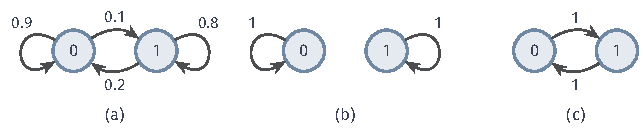
\includegraphics[width=109mm]{figures/07-probability/08-sampling-and-integration/tikz/mcerr-two-state/figure.pdf}
 \caption{两状态链的转移图，箭头上的数为转移概率。(a)$a=0.1$，$b=0.2$，不可约且非周期；(b)$a=b=0$，两个状态各自吸收，链可约；(c)$a=b=1$，不可约但周期为$2$。}
 \label{fig:mcerr-two-state}
\end{BookInlineFigure}

图~\ref{fig:mcerr-two-state}(b)与(c)是条件不成立的两种情形。可约链（$a=b=0$）就是上一节始终停在原地的例子，$\hat{I}_N=f(X^{(0)})$，既不趋于$I$，也没有正态极限。周期链（$a=b=1$）在$0,1$之间严格交替，从$\pi$出发时$\lambda=-1$，式~\eqref{eq:mcerr-two-state-lrv}给出$\sigma_{\mathrm{LR}}^{2}=0$：$N$为偶数时$\hat{I}_N$恰好等于$1/2$，误差比$N^{-1/2}$小得多，正态近似退化。从固定的状态$0$出发时，$X^{(t)}$的分布在两个单点之间来回切换，永远不趋于$\pi$，时间平均却仍然收敛。可见非周期性主要关系到边缘分布的收敛，不可约性关系到时间平均能否看到整个目标。

\paragraph{一般状态空间}
状态连续时，“以几何速度趋于目标”需要允许依赖初值的常数。若存在$r<1$与函数$M(x)$，对$\pi$几乎所有的$x$有$M(x)<\infty$，且
\begin{equation}
 d_{\mathrm{TV}}\bigl(K^{t}(x,\cdot),\pi\bigr)\leq M(x)\,r^{t},\qquad t=1,2,\dots ,
 \label{eq:mcerr-geometric-ergodic}
\end{equation}
就称链\term{几何遍历}（geometrically ergodic）。式中$t$步后的转移分布与目标之间的总变差按几何速度衰减，衰减的比例不依赖初值，起点越远只是常数$M(x)$越大。

链~\eqref{eq:mcerr-ar1}是几何遍历的。由式~\eqref{eq:mcerr-ar1-marginal}，$K^{t}(x,\cdot)$与$\pi$只差均值$\rho^{t}x$和方差$1-\rho^{2t}$。图~\ref{fig:mcerr-geo-ergodic}用数值积分算出$\rho=0.9$时的总变差：从$x=3$与$x=10$出发，曲线最终与$0.9^{t}$平行，起点越远曲线越高；从$x=0$出发，均值没有偏离，只剩方差的差别，衰减得更快，按$0.81^{t}$下降。

\begin{BookInlineFigure}
 \centering
 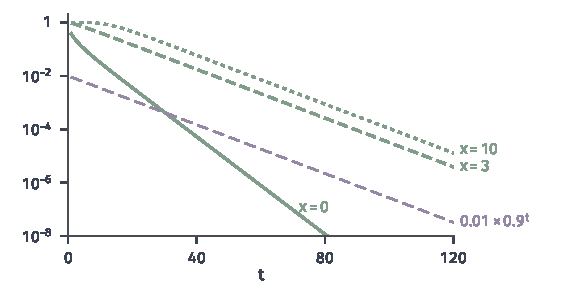
\includegraphics[width=96mm]{figures/07-probability/08-sampling-and-integration/matplotlib/mcerr-geo-ergodic/figure.pdf}
 \caption{链~\eqref{eq:mcerr-ar1}在$\rho=0.9$时，$t$步转移分布$\mathcal{N}(0.9^{t}x,1-0.81^{t})$与$\mathcal{N}(0,1)$的总变差（数值积分），绿色实线、虚线、点线分别为$x=0,3,10$；紫色虚线为参考斜率$0.01\times0.9^{t}$，纵轴为对数刻度。}
 \label{fig:mcerr-geo-ergodic}
\end{BookInlineFigure}

几何遍历配合比二阶稍强的矩条件，就足以给出正态极限。

\begin{theorem}[几何遍历链的中心极限定理]
\label{thm:mcerr-geo-clt}
设链以$\pi$为不变分布且几何遍历，$f$满足$\mathbb{E}_{\pi}\lvert f\rvert^{2+\delta}<\infty$，其中$\delta>0$。则平稳自协方差绝对可和，$\sigma_{\mathrm{LR}}^{2}<\infty$，并且链从$\pi$出发时
\begin{equation}
 \sqrt{N}\,\bigl(\hat{I}_N-I\bigr)\xrightarrow{\mathrm{d}}\mathcal{N}\bigl(0,\sigma_{\mathrm{LR}}^{2}\bigr) .
 \label{eq:mcerr-geo-clt}
\end{equation}
\end{theorem}

证明要估计相隔$k$步的两个函数值之间的依赖如何随$k$衰减，再用前面提到的鞅增量分解，篇幅较长，读者可查阅~\scite{math-meyn2009markov}。在卷九所讨论的常返条件下，结论对任意初始分布也成立。矩条件中的$\delta$一般不能取为零：对某些几何遍历的链，只满足$\mathbb{E}_{\pi}[f^{2}]<\infty$的$f$可以使$\sigma_{\mathrm{LR}}^{2}=\infty$，这类反例的构造较复杂。对链~\eqref{eq:mcerr-ar1}，$f(x)=x$或$x^{2}$的各阶矩都有限，定理适用，$f(x)=x$的极限方差就是$19$。

\paragraph{可和协方差不足以给出正态极限}
第~\ref{sec:mcerr-long-run}小节的方差极限只用了协方差绝对可和。下面的例子说明，仅有这一条不能推出正态极限。链的状态是一对$(W,Y)$。初始时$W$以各$1/2$的概率取$1$或$3$，此后永不改变；每一步$Y$重新抽取为$W\varepsilon$，其中$\varepsilon\sim\mathcal{N}(0,1)$与过去独立。转移核是
\[
 K\bigl((w,y),\cdot\bigr)=\delta_{w}\otimes\mathcal{N}(0,w^{2}) ,
\]
不变分布是“$W$各以$1/2$取$1,3$，给定$W$后$Y\sim\mathcal{N}(0,W^{2})$”。

取$f(w,y)=y$，$I=0$。平稳时
\[
 \gamma_0=\mathbb{E}[W^{2}]=5,\qquad \gamma_k=\mathbb{E}\bigl[W^{2}\varepsilon_0\varepsilon_k\bigr]=0\quad(k\geq1) ,
\]
自协方差除$\gamma_0$外全为零，绝对可和，长期方差$\sigma_{\mathrm{LR}}^{2}=5$，而且$N\operatorname{Var}(\hat{I}_N)$对每个$N$都等于$5$。可是
\[
 \sqrt{N}\,\hat{I}_N=W\cdot\frac{1}{\sqrt{N}}\sum_{t=1}^{N}\varepsilon_t ,
\]
后一个因子精确服从$\mathcal{N}(0,1)$且与$W$独立，所以$\sqrt{N}\hat{I}_N$对每个$N$都服从两个正态分布的等权混合，不是正态分布。它的四阶矩是$3\mathbb{E}[W^{4}]=123$，而方差为$5$的正态分布四阶矩是$75$。图~\ref{fig:mcerr-chain-clt}(b)中直方图中间更尖、两侧更厚，与$\mathcal{N}(0,5)$明显不同。原因是这条链可约：$W$一旦选定就再也不变，时间平均永远记得它。

\begin{BookInlineFigure}
 \centering
 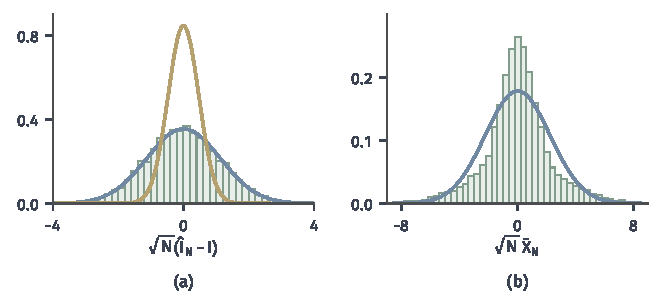
\includegraphics[width=112mm]{figures/07-probability/08-sampling-and-integration/matplotlib/mcerr-chain-clt/figure.pdf}
 \caption{链平均的极限分布。(a)两状态链$a=0.1$，$b=0.2$，从状态$0$出发，$N=2000$，$20000$条独立链（种子$3124$）的$\sqrt{N}(\hat{I}_N-1/3)$（绿色直方图），蓝线为$\mathcal{N}(0,34/27)$，黄线为误用单值方差的$\mathcal{N}(0,2/9)$；(b)可约链$(W,Y)$的$\sqrt{N}\hat{I}_N=WZ$的$20000$次抽样（绿色，种子$3125$），蓝线为$\mathcal{N}(0,5)$。}
 \label{fig:mcerr-chain-clt}
\end{BookInlineFigure}

\subsection{长期方差的估计}
\label{sec:mcerr-lrv-estimation}

即使中心极限定理成立，误差区间还需要$\sigma_{\mathrm{LR}}^{2}$的值。普通样本方差$S_N^{2}$估计的是$\gamma_0$，不是$\sigma_{\mathrm{LR}}^{2}$；用$S_N^{2}/N$作链平均的方差，在正相关时会把误差低估。下面两种估计都从同一条记录出发，分别从“分块”和“求和”两个方向逼近长期方差。

\paragraph{批均值}
由定理~\ref{thm:mcerr-long-run-limit}，长度为$b$的一段平稳记录，其平均的方差约为$\sigma_{\mathrm{LR}}^{2}/b$。若$b$远大于相关性的持续长度，相隔一段的两段平均几乎不相关。把记录切成$a$段，每段长$b$，$N=ab$，第$j$段的平均记为$\bar{Y}_j$。这$a$个段均值近似为方差$\sigma_{\mathrm{LR}}^{2}/b$的独立观测，于是它们的样本方差乘以$b$就估计了$\sigma_{\mathrm{LR}}^{2}$：
\begin{equation}
 \hat{\sigma}_{\mathrm{BM}}^{2}=\frac{b}{a-1}\sum_{j=1}^{a}\bigl(\bar{Y}_j-\hat{I}_N\bigr)^{2} .
 \label{eq:mcerr-batch-means}
\end{equation}
这种方法称为\term{批均值法}（batch means method）。$b=1$时每段只有一个值，式~\eqref{eq:mcerr-batch-means}退回普通样本方差$S_N^{2}$。

下面用一段短记录演示计算。两状态链（$a=0.1$，$b=0.2$）从不变分布出发运行$16$步（种子$3144$），$f$为状态$1$的示性函数，记录为
\[
 0,0,0,0,\ 0,0,1,0,\ 1,1,1,1,\ 1,0,0,0 .
\]
其中有六个$1$，$\hat{I}_{16}=6/16=0.375$。先算普通样本方差：六个值与平均相差$0.625$，十个值相差$-0.375$，
\[
 S_{16}^{2}=\frac{6\times0.625^{2}+10\times0.375^{2}}{15}=\frac{3.75}{15}=0.25 .
\]
再取段长$4$，分成四段，如图~\ref{fig:mcerr-batches}。段均值为
\[
 \bar{Y}_1=0,\quad \bar{Y}_2=0.25,\quad \bar{Y}_3=1,\quad \bar{Y}_4=0.25 .
\]
它们与$\hat{I}_{16}$的差的平方和为
\[
 0.375^{2}+0.125^{2}+0.625^{2}+0.125^{2}=0.5625 ,
\]
代入式~\eqref{eq:mcerr-batch-means}，
\[
 \hat{\sigma}_{\mathrm{BM}}^{2}=\frac{4}{3}\times0.5625=0.75 .
\]
两种估计给出的标准误差分别是
\[
 \sqrt{0.25/16}=0.125,\qquad \sqrt{0.75/16}=0.217 .
\]
真实的$\sigma_{\mathrm{LR}}^{2}=1.259$，平稳时的标准误差为$\sqrt{1.259/16}=0.281$。普通样本方差把它低估了一半以上；批均值的方向是对的，但只有四段，估计本身很粗糙。

\begin{BookInlineFigure}
 \centering
 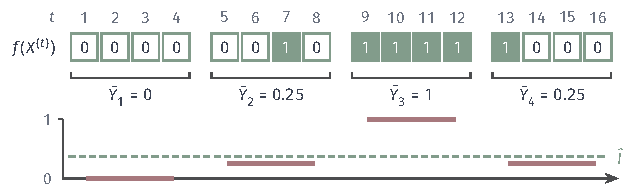
\includegraphics[width=107mm]{figures/07-probability/08-sampling-and-integration/tikz/mcerr-batches/figure.pdf}
 \caption{批均值的计算。上排为两状态链$16$步的函数值$f(X^{(t)})$（绿色方格为$1$），按长度$4$分成四段；下方红色横线为各段平均$\bar{Y}_j$，绿色虚线为总平均$\hat{I}=0.375$。段均值之间的离散程度反映了长期方差。}
 \label{fig:mcerr-batches}
\end{BookInlineFigure}

\paragraph{截断的自协方差和}
另一条路是直接按定义~\ref{def:mcerr-long-run}求和。由记录估计自协方差
\[
 \hat{\gamma}_k=\frac1N\sum_{t=1}^{N-k}\bigl(f(X^{(t)})-\hat{I}_N\bigr)\bigl(f(X^{(t+k)})-\hat{I}_N\bigr) ,
\]
再截断到$L$步：
\begin{equation}
 \hat{\sigma}_{L}^{2}=\hat{\gamma}_0+2\sum_{k=1}^{L}w_k\,\hat{\gamma}_k .
 \label{eq:mcerr-truncated-sum}
\end{equation}
权重$w_k=1$是直接截断；取$w_k=1-k/(L+1)$可以保证估计非负。不能对所有$k\leq N-1$求和：大$k$的$\hat{\gamma}_k$只由很少几对数据算出，噪声很大，全部加起来以后误差不随$N$缩小。

\paragraph{块长与截断的选择}
两种估计都面临同一个取舍。块长$b$或截断$L$太小，漏掉了尚未衰减的相关，估计偏低；太大，段数太少或加入太多噪声项，估计波动很大。图~\ref{fig:mcerr-lrv-estimates}在链~\eqref{eq:mcerr-ar1}（$\rho=0.9$）上用十条长度$2^{16}$的记录演示：$b=1$时批均值约为$\gamma_0=1$；$b=128$时十次的平均为$17.7$，仍偏低；$b=512$时平均为$18.7$，十次的标准差为$1.6$；$b=4096$时只剩$16$段，标准差增大到$7.9$。截断和的情形相同，$L$约为$60$时最稳定。

\begin{BookInlineFigure}
 \centering
 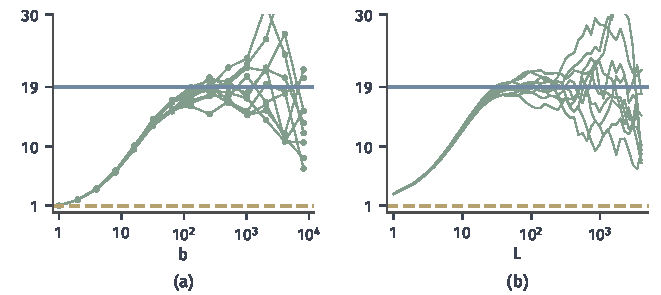
\includegraphics[width=112mm]{figures/07-probability/08-sampling-and-integration/matplotlib/mcerr-lrv-estimates/figure.pdf}
 \caption{长期方差的两种估计，链~\eqref{eq:mcerr-ar1}，$\rho=0.9$，$f(x)=x$，十条长度$N=2^{16}$的平稳记录（绿线，种子$3130$）。(a)批均值估计随块长$b$的变化；(b)直接截断的自协方差和随截断步数$L$的变化。蓝线为$\sigma_{\mathrm{LR}}^{2}=19$，黄色虚线为$\gamma_0=1$，横轴为对数刻度。}
 \label{fig:mcerr-lrv-estimates}
\end{BookInlineFigure}

要使估计一致，$b$与$a=N/b$都必须随$N$趋于无穷，例如$b$取$\sqrt{N}$的量级；截断和则要求$L\to\infty$且$L/N\to0$。此外还需要链以足够快的速度遍历，$f$满足比二阶更高的矩条件。证明需要把链的部分和与连续时间的随机路径作细致比较，超出本卷范围。

\paragraph{链平均的误差区间}
把三块拼起来：只有在链平均满足中心极限定理、$\sigma_{\mathrm{LR}}^{2}>0$且$\hat{\sigma}^{2}$是一致估计时，由Slutsky定理，
\[
 \frac{\sqrt{N}\,(\hat{I}_N-I)}{\hat{\sigma}}\xrightarrow{\mathrm{d}}\mathcal{N}(0,1) ,
\]
从而区间$\hat{I}_N\pm z\hat{\sigma}/\sqrt{N}$的覆盖概率趋于$1-\alpha$。这里的$\hat{\sigma}^{2}$是$\hat{\sigma}_{\mathrm{BM}}^{2}$或$\hat{\sigma}_{L}^{2}$，不能用$S_N^{2}$代替。三个条件中任何一个不成立，区间都没有保证：可约链没有正态极限，周期链可能$\sigma_{\mathrm{LR}}^{2}=0$，块长不当则方差估计不一致。

\subsection{运行诊断的边界}
\label{sec:mcerr-diagnostics}

上面的条件涉及链的遍历性质，通常无法从记录中验证。实践中用一些运行诊断来发现问题，它们各有用处，也各有盲区。

\paragraph{一个双峰目标}
取$\pi$为$\mathcal{N}(-5,1)$与$\mathcal{N}(5,1)$的等权混合，$f(x)=x$，$I=0$。用第~\ref{chap:sample-generation}章的随机游走Metropolis算法：从当前状态$x$提出候选$y=x+\eta$，$\eta\sim\mathcal{N}(0,1)$，以概率$\min\{1,\tilde{p}(y)/\tilde{p}(x)\}$接受，否则留在$x$，其中$\tilde{p}$是$\pi$的密度。这条链以$\pi$为不变分布，并且候选可以到达任何位置，理论上能在两个峰之间往返。问题在于两峰之间密度很低：$x=0$处的密度只有峰值的$2\mathrm{e}^{-12.5}\approx7\times10^{-6}$倍，每一步只能移动一个单位左右，穿越低谷需要连续多次接受向下的移动，这几乎不会发生。

图~\ref{fig:mcerr-bimodal-traces}(a)从$-7,-3,3,7$出发运行四条链，每条$5000$步（种子$3131$），接受率约为$0.70$。四条链没有一次穿过$0$：两条留在左峰，平均为$-5.00$与$-5.01$；两条留在右峰，平均为$5.05$与$4.95$。链间的分歧明白地暴露了问题。把四条链合在一起，平均为$-0.004$，碰巧接近$0$，但这只是因为初值恰好两边各两个；若三条从左边出发，合并平均就在$-2.5$附近。两峰各占多少质量，这些记录完全没有测量到。

图(b)把四条链都放在左侧，从$-7,-6,-4,-3$出发（种子$3132$）。四条链的平均分别为$-4.98,-4.98,-5.03,-4.94$，彼此一致；轨迹看起来平稳，运行平均早已停住，每条链的估计有效样本量也不小。所有诊断都通过了，答案却是$-4.98$而不是$0$。

\begin{BookInlineFigure}
 \centering
 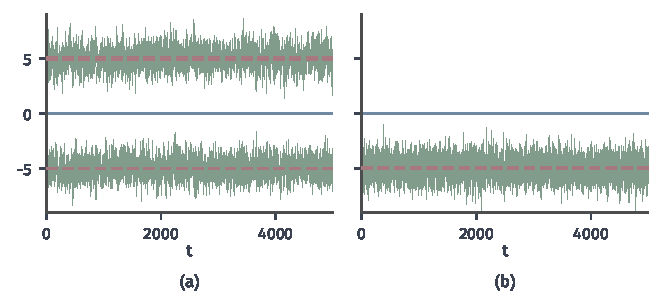
\includegraphics[width=112mm]{figures/07-probability/08-sampling-and-integration/matplotlib/mcerr-bimodal-traces/figure.pdf}
 \caption{双峰目标$\frac12\mathcal{N}(-5,1)+\frac12\mathcal{N}(5,1)$上的随机游走Metropolis链，每条$5000$步。绿线为轨迹，红色虚线为每条链的平均，蓝线为$I=0$。(a)从$-7,-3,3,7$出发（种子$3131$）；(b)从$-7,-6,-4,-3$出发（种子$3132$）。}
 \label{fig:mcerr-bimodal-traces}
\end{BookInlineFigure}

\paragraph{各种诊断能看到什么}
表~\ref{tab:mcerr-diagnostics}总结了常用的几种诊断。比较多次运行时，常同时看链间平均的差异与链内的波动：若链间差异远大于链内波动所能解释的范围，说明各链还没有忘掉初值或停在不同区域。\term{轨迹图}（trace plot）即状态随步数的曲线，\term{运行均值}（running mean）即前$t$步平均随$t$的曲线。

\begin{BookInlineTable}
 \centering
 \caption{运行诊断的作用与盲区}
 \label{tab:mcerr-diagnostics}
 \begin{tabular}{p{25mm}p{36mm}p{36mm}}
  \toprule
  诊断 & 能发现 & 不能发现 \\
  \midrule
  不同初值的多次运行 & 初值影响，停在不同区域 & 所有初值都未到达的区域 \\
  轨迹图 & 趋势，缓慢移动，停滞 & 从未访问的区域 \\
  运行均值 & 尚未稳定的漂移 & 稳定在错误值上 \\
  估计的有效样本量 & 强相关，方差估计不稳 & 只在局部区域混合良好 \\
  \bottomrule
 \end{tabular}
\end{BookInlineTable}

这些诊断共同的盲区是：有限的记录只能告诉我们链去过哪里，不能告诉我们还有哪里没去。双峰例子里，记录中没有任何信息提示右边还有一半质量；第~\ref{sec:mcerr-asymptotic-interval}小节的稀有大贡献是同一现象在独立样本中的版本。所以诊断的结论只能是否定性的：诊断失败说明有问题，诊断通过不说明没有问题。误差区间所需的遍历性与矩条件，需要从目标与转移的结构分析得到，例如知道目标的峰在哪里，或者证明转移满足几何遍历；运行诊断不能替代这些理论条件。


\section{整组随机化的误差}
\label{sec:mcerr-replication}

有些采样方法一次产生一组彼此相关的点：每个点单独看都服从目标分布，但点与点之间被有意安排，使整组覆盖得更均匀。第~\ref{chap:variance-reduction}章的拉丁超立方采样与随机化准Monte Carlo都属于这一类。这样的组内平均无偏，方差却不能用独立公式计算，同一组点的样本方差也不反映它。办法是把整组当作一个观测单位，独立地重复整个构造。

\paragraph{整体平移的网格}
用一个最简单的构造说明。目标仍是$I=\int_0^1\mathrm{e}^{u}\,\mathrm{d}u$。取$n$个等距点$a_i=(i-1)/n$，$i=1,\dots,n$，再取一个$\Delta\sim\operatorname{Unif}(0,1)$，把所有点一起平移并按模$1$回绕：
\[
 U_i=(a_i+\Delta)\bmod1 .
\]
对固定的$a\in[0,1)$与$s\in[0,1]$，使$(a+\Delta)\bmod1\leq s$的$\Delta$构成$[0,1)$中总长度为$s$的一个或两个区间，所以每个$U_i$都服从$\operatorname{Unif}(0,1)$。由第~\ref{sec:mcerr-estimator}节，组平均
\[
 Q=\frac1n\sum_{i=1}^{n}f(U_i)
\]
是$I$的无偏估计。但这些点完全不独立：知道一个点，就知道了整组。

$n=4$时，组平均只依赖$\Delta'=\Delta\bmod\tfrac14$：四个点就是$\Delta'+j/4$，$j=0,1,2,3$。对$f(u)=\mathrm{e}^{u}$，等比求和给出
\begin{equation}
 Q=\frac{\mathrm{e}^{\Delta'}}{4}\sum_{j=0}^{3}\mathrm{e}^{j/4}=c\,\mathrm{e}^{\Delta'},\qquad c=\frac{\mathrm{e}-1}{4(\mathrm{e}^{1/4}-1)}=1.5124 .
 \label{eq:mcerr-shift-q}
\end{equation}
四个点均匀地分布在$[0,1)$上，相互弥补，$\operatorname{Var}(Q)=0.01536$；同样四个独立均匀点的平均，方差是$\sigma_f^{2}/4=0.0605$，大了约四倍。组内的依赖正是精度提高的来源，也正是它使独立公式失效。

\subsection{组间方差}
\label{sec:mcerr-between-var}

固定每组点数$n$，用独立的随机数重复同一个随机化规则$R$次，得到组估计$Q_1,\dots,Q_R$。它们独立同分布，每一个都是一次完整构造的结果。

\begin{theorem}[组间方差估计]
\label{thm:mcerr-between-var}
设$Q_1,\dots,Q_R$独立同分布，$\mathbb{E}[Q_1]=I$，$\mathbb{E}[Q_1^{2}]<\infty$，$R\geq2$。令
\begin{equation}
 \bar{Q}=\frac1R\sum_{r=1}^{R}Q_r,\qquad s_Q^{2}=\frac{1}{R-1}\sum_{r=1}^{R}\bigl(Q_r-\bar{Q}\bigr)^{2} .
 \label{eq:mcerr-between}
\end{equation}
则$\mathbb{E}[\bar{Q}]=I$，并且
\begin{equation}
 \operatorname{Var}(\bar{Q})=\frac{\operatorname{Var}(Q_1)}{R},\qquad \mathbb{E}\Bigl[\frac{s_Q^{2}}{R}\Bigr]=\operatorname{Var}(\bar{Q}) .
 \label{eq:mcerr-between-unbiased}
\end{equation}
\end{theorem}

\begin{proof}
前两条是独立同分布变量平均的期望与方差，与定理~\ref{thm:mcerr-iid-bound}的证明相同。记$v=\operatorname{Var}(Q_1)$。把每一项写成$Q_r-\bar{Q}=(Q_r-I)-(\bar{Q}-I)$，展开平方和，并利用$\sum_r(Q_r-I)=R(\bar{Q}-I)$，
\[
 \sum_{r=1}^{R}\bigl(Q_r-\bar{Q}\bigr)^{2}=\sum_{r=1}^{R}(Q_r-I)^{2}-R\,(\bar{Q}-I)^{2} .
\]
取期望，第一项为$Rv$，第二项为$R\cdot v/R=v$，所以
\[
 \mathbb{E}\Bigl[\sum_{r=1}^{R}\bigl(Q_r-\bar{Q}\bigr)^{2}\Bigr]=(R-1)\,v .
\]
除以$R-1$得$\mathbb{E}[s_Q^{2}]=v$，再除以$R$即得结论。
\end{proof}

定理只用到组与组之间的独立，对组内点的依赖没有任何要求。这正是需要的分工：组内怎样安排由设计决定，误差由组间的波动来度量。反过来，把$nR$个点混在一起求样本方差再除以$nR$，相当于假装这些点彼此独立，没有依据。

\paragraph{四组的计算}
取$n=4$，$R=4$，四次平移为
\[
 \Delta_1=0.37,\quad \Delta_2=0.81,\quad \Delta_3=0.19,\quad \Delta_4=0.64 ,
\]
如图~\ref{fig:mcerr-group-shift}(a)。按模$\tfrac14$约化，$\Delta'$依次为$0.12,0.06,0.19,0.14$。代入式~\eqref{eq:mcerr-shift-q}，
\[
 Q_1=1.7053,\quad Q_2=1.6060,\quad Q_3=1.8289,\quad Q_4=1.7397 .
\]
总平均为$\bar{Q}=1.7200$，与$I=1.7183$相差$0.0017$。各组与总平均的差是$-0.0147,-0.1140,0.1089,0.0198$，由式~\eqref{eq:mcerr-between}，
\[
 s_Q^{2}=0.008491,\qquad \frac{s_Q^{2}}{R}=0.002123,\qquad \sqrt{s_Q^{2}/R}=0.0461 .
\]
真实的$\operatorname{Var}(\bar{Q})=0.01536/4=0.00384$，标准差为$0.0620$；只有四组时，估计值$0.0461$偏小，但这是随机波动，不是系统偏差。

若把$16$个函数值当作独立样本，它们的样本方差为$0.2483$，除以$16$得$0.01552$，标准误差$0.1246$，是真实值的两倍。它实际上估计的是$16$个独立点的方差$\sigma_f^{2}/16$，完全没有反映网格带来的改进。这里组内点相互弥补，独立公式高估了误差；若组内点彼此相似，例如一段链记录，独立公式就会低估误差。两个方向的错误都来自同一个原因：用组内的离散程度代替了组间的波动。

图~\ref{fig:mcerr-group-shift}(b)把整个实验（每次$R=4$组）重复$5000$次。正确估计$s_Q^{2}/R$的平均为$0.00382$，与真实值$0.00384$一致，但分布很宽，因为每次只有四个组估计；混合估计集中在$0.0159$附近，稳定地错了四倍。

\begin{BookInlineFigure}
 \centering
 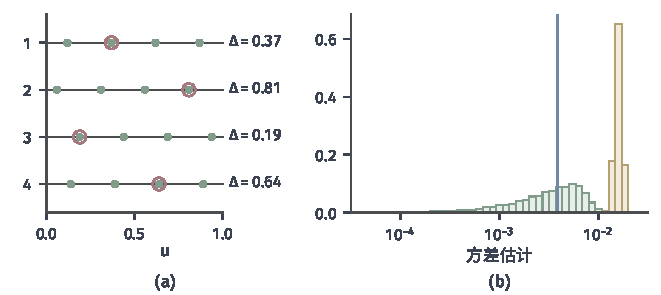
\includegraphics[width=112mm]{figures/07-probability/08-sampling-and-integration/matplotlib/mcerr-group-shift/figure.pdf}
 \caption{整体平移网格估计$\int_0^1\mathrm{e}^{u}\,\mathrm{d}u$，每组$n=4$点。(a)四组点（绿点），红圈为各组的平移量$\Delta_r$；(b)整个实验（$R=4$）重复$5000$次（种子$3133$）：绿色为$s_Q^{2}/R$的分布，黄色为把$16$个值当作独立样本的估计，蓝线为真实的$\operatorname{Var}(\bar{Q})=0.00384$，横轴为对数刻度。}
 \label{fig:mcerr-group-shift}
\end{BookInlineFigure}

\subsection{渐近误差区间}
\label{sec:mcerr-replication-interval}

组估计$Q_1,\dots,Q_R$是独立同分布的观测，第~\ref{sec:mcerr-asymptotic-interval}小节的结论可以原样搬过来，只是把“样本”换成“整组”，把样本数$N$换成重复数$R$。若$n$固定，$0<\operatorname{Var}(Q_1)<\infty$，则由定理~\ref{thm:mcerr-iid-clt}，$R\to\infty$时
\begin{equation}
 \frac{\sqrt{R}\,(\bar{Q}-I)}{s_Q}\xrightarrow{\mathrm{d}}\mathcal{N}(0,1) ,
 \label{eq:mcerr-replication-clt}
\end{equation}
区间$\bar{Q}\pm z\,s_Q/\sqrt{R}$的覆盖概率趋于$1-\alpha$。

上面的四组给出区间
\[
 1.7200\pm1.96\times0.0461=[1.6297,\,1.8103] ,
\]
包含$I$。但$R=4$离“$R\to\infty$”很远。由式~\eqref{eq:mcerr-shift-q}，$Q$是$\Delta'$的指数函数，取值在一个有界区间内，并不服从正态分布。用$20$万次重复实验（种子$3134$）估计，这个区间的实际覆盖概率在$R=4$时为$0.840$，$R=10$时为$0.917$，$R=30$时为$0.939$，$R=100$时为$0.947$。

对少量重复，常见的做法是把$z$换成自由度为$R-1$的t分布分位数，$R=4$时为$3.182$。若各组估计恰好服从正态分布，这能给出精确的覆盖概率；但组估计一般不是正态的，本例中这样做的覆盖概率是$0.929$，仍低于$0.95$。所以少量整组重复只能给出近似的误差范围，不提供有限样本下的精确覆盖保证。

这一节的结论可以概括为两条。第一，组内点边缘分布正确只保证无偏，不意味着它们彼此独立，组内的样本方差不衡量估计的误差。第二，独立重复的整组是误差估计的基本单位，误差区间的可靠程度由重复数$R$决定，而不是由总点数$nR$决定。第~\ref{chap:variance-reduction}章设计组内结构以减小$\operatorname{Var}(Q)$时，都按这里的方式估计误差。


\section{本章小结}
\label{sec:mcerr-summary}

Monte Carlo估计$\hat{I}_N$的误差总是分成偏差与随机波动两部分。偏差只取决于各个样本的分布是否等于$\pi$，与样本是否独立无关；波动取决于样本之间的依赖与被积函数的矩。两部分必须分别评价：增加样本数只压低波动，从不消除偏差，而偏差又无法从输出本身读出。

\paragraph{各种来源的误差}
表~\ref{tab:mcerr-summary}按样本来源列出本章的主要结论。

\begin{BookInlineTable}
 \centering
 \caption{不同样本来源下的误差}
 \label{tab:mcerr-summary}
 \begin{tabular}{lll}
  \toprule
  样本来源 & 偏差 & 波动的尺度 \\
  \midrule
  独立、精确 & 零 & $\sigma_f^{2}/N$，需二阶矩 \\
  独立、近似$\tilde{\pi}$ & $\mathbb{E}_{\tilde{\pi}}f-\mathbb{E}_{\pi}f$，不随$N$变 & $\operatorname{Var}_{\tilde{\pi}}(f)/N$ \\
  链、从一般初值出发 & 由边缘分布的收敛速度控制 & 同下 \\
  链、平稳 & 零 & 渐近为$\sigma_{\mathrm{LR}}^{2}/N$ \\
  整组随机化 & 零（各点边缘正确时） & $\operatorname{Var}(Q)/R$ \\
  \bottomrule
 \end{tabular}
\end{BookInlineTable}

\paragraph{保证的类型}
独立样本有两类保证。Chebyshev界对每个$N$成立，只需二阶矩，但偏松；渐近误差区间更紧，但只在$N\to\infty$时给出名义覆盖，稀有的大贡献可以使所需的$N$大到无法从样本中察觉。只有一阶矩时大数律仍成立，但误差可以按慢于$N^{-1/2}$的速度缩小。

近似生成的偏差由总变差控制，前提是被积函数有界；无界时还要控制两种分布的尾部或矩。近似转移先要确认存在不变分布，再估计它与$\pi$的差别。

链平均的初值偏差需要边缘分布趋于$\pi$的速度估计，舍弃初始一段只有在这种估计下才有依据，对无界函数还需要一致可积。平稳链平均的方差由自协方差决定，长期方差是它的极限，有效样本量是它的换算，三者都依赖被积函数。链平均的误差区间同时需要中心极限定理、正的长期方差和一致的长期方差估计；运行诊断只能发现问题，不能证明链已遍历目标。

一次产生一组相关点的方法，以独立重复的整组为观测单位，用组间的样本方差估计误差，可靠程度由重复数决定。

\paragraph{与后续各章的关系}
第~\ref{chap:variance-reduction}章改变抽样分布、估计公式或抽样机制来减小波动，每一种改变都会改变估计量的分布，因而都要按本章的方式重新检查偏差、矩条件和样本之间的依赖。第~\ref{chap:expectation-gradient-estimation}章估计期望的导数时，近似采样带来的偏差同样不能靠样本数消除。第~\ref{chap:sampling-budget-method-selection}章在给定预算下分配样本，所比较的正是本章给出的偏差与方差。


\chapter{方差控制}
\label{chap:variance-reduction}

设$X\sim\operatorname{Exp}(1)$，要算$I=\mathbb{P}(X>4)=\mathrm{e}^{-4}\approx0.0183$。按第~\ref{chap:monte-carlo-integration-error}章的做法，独立生成$n$个$X_i$，数一数有多少个超过$4$，再除以$n$。每个样本的示性值方差是$I(1-I)\approx0.0180$，于是相对误差约为
\[
 \frac{\sqrt{I(1-I)/n}}{I}=\sqrt{\frac{1-I}{nI}} .
\]
$n=1000$时这个量约为$0.23$：一千个样本里平均只有$18$个落进尾部，估计值上下浮动两成多。要把相对误差压到$1\%$，需要约$5.4\times10^{5}$个样本。

问题出在样本的去向。绝大多数样本落在$[0,4]$里，对积分没有任何贡献，只有极少数样本决定了估计值。如果能让更多样本落进尾部，再按某种方式扣回多抽的比例，同样的计算量就能得到更稳定的结果。另一个例子是
\[
 I=\int_0^1\mathrm{e}^{u}\,\mathrm{d}u=\mathrm{e}-1 .
\]
被积函数随$u$单调增加，大部分波动只是“$u$偏大还是偏小”造成的，这部分波动有办法预先抵消。

本章固定待算的积分，研究怎样重新安排随机计算，使得同样的预算下估计的方差更小。第~\ref{sec:vr-comparison}节先说明比较的口径：方差要与成本一起比较，有偏的估计还要计入偏差。随后分三个方向。改变分布：从另一个分布抽样，再用权重恢复原积分。改变计算公式：减去期望已知的辅助量，或把一部分随机性用条件平均消去。改变抽样机制：把基础随机数按层、按点集或成对地安排，控制样本落在哪里以及样本之间的协方差。

尾概率和$\mathrm{e}^{u}$两个例子贯穿全章，另有几个专门的例子说明方法的失效情形。全章用到第~\ref{chap:conditional-expectation}章的条件期望与全方差公式、第~\ref{chap:laws-of-large-numbers}章的大数律、第~\ref{chap:central-limit-theorem}章的中心极限定理，以及第~\ref{chap:sample-generation}章的生成方法；误差的基本分解取自第~\ref{chap:monte-carlo-integration-error}章。

\section{方差比较的条件}
\label{sec:vr-comparison}

说一种方法“方差更小”之前，先要讲清楚和什么比、在什么预算下比。一种方法每个样本的方差只有原来的一半，但每个样本的计算时间是原来的三倍，它在同样的时间内得到的结果反而更差。另一种方法方差很小，却有偏差，单看方差会高估它。本节规定全章比较估计量的口径。

\paragraph{基准}
前两章把目标分布记作$\pi$；本章常要同时处理目标与另一个抽样分布的密度，因此把目标分布记作$P$，密度记作$p$。

固定样本空间$\mathcal{X}$上的概率分布$P$与函数$f$，设$f$在$P$下可积，待算的积分是
\[
 I=\mathbb{E}_P[f(X)] .
\]
基准是第~\ref{chap:monte-carlo-integration-error}章的独立样本平均：$X_1,\dots,X_n$独立且都服从$P$，
\[
 \hat{I}_n=\frac1n\sum_{i=1}^{n}f(X_i) .
\]
估计$\hat{I}_n$无偏；若再有$\mathbb{E}_P[f(X)^2]<\infty$，记$\sigma^2=\operatorname{Var}_P(f(X))$，则$\operatorname{Var}(\hat{I}_n)=\sigma^2/n$。本章的方法都在这一基准上改动，并且大多保留一个结构：估计量由若干个相互独立的“单元”平均而成。单元可以是一个样本，也可以是一对样本、一组分层样本或一个随机化点集。

\paragraph{方差乘成本}
设一个单元输出随机变量$Y$，满足$\mathbb{E}[Y]=I$与$v=\operatorname{Var}(Y)<\infty$，生成一个单元的平均成本为$c>0$。成本按实际计算计入：生成基础随机数、把它变换成样本、求$f$的值，以及权重、辅助函数、密度等额外计算。总预算为$C$时可以算$m=C/c$个独立单元（暂不计取整），平均值的方差为
\begin{equation}
 \operatorname{Var}\Bigl(\frac1m\sum_{k=1}^{m}Y_k\Bigr)=\frac{v}{m}=\frac{v\,c}{C} .
 \label{eq:vr-work-variance}
\end{equation}
预算固定时，决定精度的是乘积$v\,c$，而不是$v$本身。两种无偏方法A与B相比，定义B相对于A的\term{相对效率}（relative efficiency）为
\begin{equation}
 \operatorname{eff}(\mathrm{B}:\mathrm{A})=\frac{v_{\mathrm{A}}\,c_{\mathrm{A}}}{v_{\mathrm{B}}\,c_{\mathrm{B}}} .
 \label{eq:vr-relative-efficiency}
\end{equation}
它的含义是：要达到同样的方差，A所需的预算是B的$\operatorname{eff}(\mathrm{B}:\mathrm{A})$倍。

\paragraph{预备成本}
有些方法在正式计算前要做一次准备，例如试运行、拟合一个分布或估计一个系数。若准备的成本是固定的$C_0$，正式计算只剩$C-C_0$，式~\eqref{eq:vr-work-variance}成为$v\,c/(C-C_0)$。于是预算较小时准备可能得不偿失，预算较大时它的分摊成本才变得可以忽略。

\paragraph{尾概率的例子}
回到导言的$I=\mathbb{P}(X>4)$。直接平均记为方法A，第~\ref{sec:vr-change-distribution}节改从另一个分布抽样并乘以权重的方法记为B，在那里会算出B的单样本方差。两种方法的参数为
\[
 v_{\mathrm{A}}=0.01798,\quad c_{\mathrm{A}}=1;\qquad v_{\mathrm{B}}=0.001749,\quad c_{\mathrm{B}}=1.5 .
\]
其中$v_{\mathrm{A}}=I(1-I)$，$c_{\mathrm{B}}=1.5$假设求权重使单样本成本增加一半；另设选择抽样分布的试运行花费$C_0=2000$。不计准备时，
\[
 \operatorname{eff}(\mathrm{B}:\mathrm{A})=\frac{0.01798\times1}{0.001749\times1.5}\approx6.9 .
\]
计入准备时，两者方差相等的预算由下式确定：
\[
 \frac{0.01798}{C}=\frac{0.001749\times1.5}{C-2000} .
\]
解得$C\approx2342$。图~\ref{fig:vr-budget-crossover}画出两种方法的相对均方根误差随预算的变化：预算低于交点时，准备几乎吃掉全部预算，新方法更差；预算到$10^{5}$时，直接平均的相对误差约为$2.3\%$，新方法约为$0.89\%$。

\begin{BookInlineFigure}
 \centering
 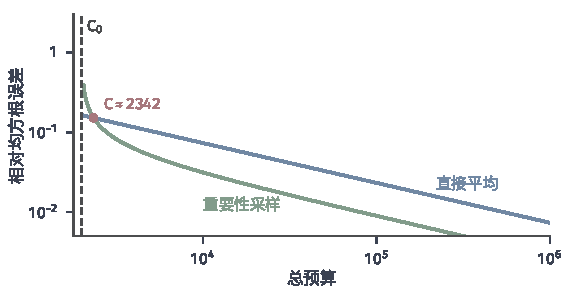
\includegraphics[width=96mm]{figures/07-probability/08-sampling-and-integration/matplotlib/vr-budget-crossover/figure.pdf}
 \caption{$I=\mathbb{P}(X>4)$，$X\sim\operatorname{Exp}(1)$，相对均方根误差$\sqrt{v\,c/(C-C_0)}/I$随总预算$C$的变化，双对数坐标。蓝线为直接平均（$v=0.01798$，$c=1$，$C_0=0$），绿线为第~\ref{sec:vr-change-distribution}节的加权估计（$v=0.001749$，$c=1.5$，$C_0=2000$），虚线标出$C_0$，红点为两者相等的预算。}
 \label{fig:vr-budget-crossover}
\end{BookInlineFigure}

\paragraph{二阶矩要逐项核对}
式~\eqref{eq:vr-work-variance}要求$v<\infty$。本章的每一种改动都会改变单元的形式：乘以权重、减去辅助量、换成条件平均或成对平均。原积分存在只说明$\mathbb{E}[\lvert Y\rvert]<\infty$，不说明$\mathbb{E}[Y^2]<\infty$。方差为无穷时，式~\eqref{eq:vr-relative-efficiency}失去意义，误差也不再按$m^{-1/2}$缩小。所以每引入一种估计量，都要单独检查它的二阶矩。

\paragraph{有偏的估计}
有些估计量不是无偏的，例如用同一批样本估计系数再代回，或者用两个平均值的比值作估计。这时比较的对象是均方误差，由第~\ref{chap:monte-carlo-integration-error}章，
\[
 \mathbb{E}\bigl[(\hat{I}-I)^2\bigr]=\bigl(\mathbb{E}[\hat{I}]-I\bigr)^2+\operatorname{Var}(\hat{I}) .
\]
常见的情形是偏差与$1/n$同阶而方差与$1/n$同阶，偏差的平方是$1/n^2$阶，样本量大时可以忽略。但样本量小时两者可能相当。另一个陷阱是：把内部样本量固定的有偏估计独立重复$R$次再平均，方差按$1/R$缩小，偏差却原样保留。这类估计的偏差要按内部样本量单独分析。

\paragraph{三个改动的位置}
一次随机计算可以看成一条流水线：基础随机数$\bm{U}$经生成映射$T$变成样本$X=T(\bm{U})$，求值得到$f(X)$，再取平均。图~\ref{fig:vr-three-routes}标出本章三类方法改动的位置。改变分布作用在生成这一步，样本改从别的分布抽取；改变计算公式作用在求值这一步，被平均的量不再是$f(X)$；改变抽样机制作用在基础随机数上，改变的是各个$\bm{U}$之间的安排。三类改动可以组合，组合后要按本节的口径重新检查期望、二阶矩和成本；在实际预算下怎样分配试运行与正式计算、怎样在方法之间取舍，由第~\ref{chap:sampling-budget-method-selection}章统一讨论。

\begin{BookInlineFigure}
 \centering
 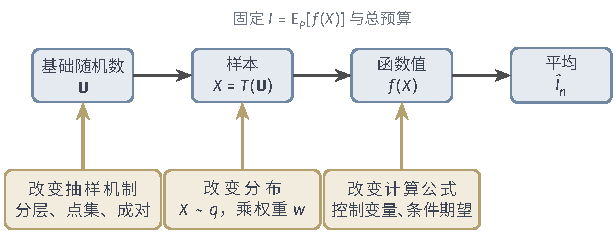
\includegraphics[width=104mm]{figures/07-probability/08-sampling-and-integration/tikz/vr-three-routes/figure.pdf}
 \caption{一次随机计算的流水线与三类方差控制方法的作用位置。上排是基础随机数、样本、函数值与平均；下排黄色框分别改动基础随机数的安排、样本的分布与被平均的量。积分$I$与总预算在比较中保持不变。}
 \label{fig:vr-three-routes}
\end{BookInlineFigure}


\section{改变分布}
\label{sec:vr-change-distribution}

尾概率$\mathbb{P}(X>4)$难算，是因为按$P$抽样时样本几乎从不进入尾部。一个自然的想法是换一个更常落进尾部的分布来抽样。这样抽到的样本不再服从$P$，直接求平均会高估尾概率；但每个样本被“多抽”了多少是已知的，可以按比例把它的贡献折回去。

用质量的语言说：$P$把单位质量按密度$p$摊在样本空间上，新分布把同样的单位质量按密度$q$重新摊开。一个按$q$抽到的样本点$x$，代表它附近$q$那么多的质量；要让它替$P$说话，就要给它乘上$p(x)/q(x)$。$q$比$p$大的地方样本来得勤，每个样本分量轻；$q$比$p$小的地方样本来得少，每个样本分量重。这种做法称为\term{重要性采样}（importance sampling）。本节先验证折算的公式，再研究怎样选择新分布，最后处理目标密度只知道到一个常数倍的情形。

\subsection{换测度与权重}
\label{sec:vr-change-of-measure}

设样本空间$\mathcal{X}$上有参考测度$\mu$：$\mathcal{X}=\mathbb{R}^{d}$时取Lebesgue测度，$\mathcal{X}$可数时取计数测度。目标分布$P$关于$\mu$有密度$p$，另取一个容易抽样、密度$q$可以计算的分布$Q$，称为建议分布（第~\ref{chap:sample-generation}章的拒绝采样已经用过这个名称）。

\begin{definition}[重要性采样估计]
\label{def:vr-importance-sampling}
设$\{x:f(x)p(x)\neq0\}\subseteq\{x:q(x)>0\}$（允许相差一个$\mu$零测集）。称
\begin{equation}
 w(x)=\begin{cases}p(x)/q(x), & q(x)>0,\\ 0, & q(x)=0\end{cases}
 \label{eq:vr-importance-weight}
\end{equation}
为\term{重要性权重}（importance weight）。对独立且都服从$Q$的$X_1,\dots,X_n$，称
\begin{equation}
 \hat{I}_n^{\mathrm{IS}}=\frac1n\sum_{i=1}^{n}f(X_i)\,w(X_i)
 \label{eq:vr-is-estimator}
\end{equation}
为$I$的重要性采样估计。
\end{definition}

定义中的包含关系称为覆盖条件：凡是$fp$不为零、对积分有贡献的地方，建议分布都必须有正密度。$q=0$处的权重取值无关紧要，因为按$Q$抽样几乎不会落到那里。

\begin{theorem}[换测度恒等式]
\label{thm:vr-change-of-measure}
设覆盖条件成立且$\mathbb{E}_P[\lvert f(X)\rvert]<\infty$。则$f w$在$Q$下可积，
\begin{equation}
 \mathbb{E}_Q[f(X)w(X)]=\mathbb{E}_P[f(X)]=I ,
 \label{eq:vr-change-of-measure}
\end{equation}
所以$\hat{I}_n^{\mathrm{IS}}$无偏，并且当$n\to\infty$时$\hat{I}_n^{\mathrm{IS}}\xrightarrow{\mathrm{a.s.}}I$。若进一步有
\begin{equation}
 M(q)=\mathbb{E}_Q\bigl[f(X)^2w(X)^2\bigr]=\int_{\{q>0\}}\frac{f^2p^2}{q}\,\mathrm{d}\mu<\infty ,
 \label{eq:vr-is-second-moment}
\end{equation}
则
\begin{equation}
 \operatorname{Var}\bigl(\hat{I}_n^{\mathrm{IS}}\bigr)=\frac{M(q)-I^2}{n} .
 \label{eq:vr-is-variance}
\end{equation}
\end{theorem}

\begin{proof}
记$S=\{q>0\}$。在$S$上$w\,q=p$，所以
\[
 \mathbb{E}_Q\bigl[\lvert f w\rvert\bigr]=\int_S\lvert f\rvert\frac{p}{q}\,q\,\mathrm{d}\mu=\int_S\lvert f\rvert p\,\mathrm{d}\mu .
\]
由覆盖条件，$S$之外$\lvert f\rvert p$几乎处处为零，右边等于$\mathbb{E}_P[\lvert f\rvert]<\infty$。去掉绝对值重复同样的计算，得到式~\eqref{eq:vr-change-of-measure}。

于是$f(X_i)w(X_i)$是独立同分布、期望为$I$的可积变量。对它们的平均取期望得到无偏性；由第~\ref{chap:laws-of-large-numbers}章的强大数律得到几乎必然收敛。二阶矩有限时，单项方差为$M(q)-I^2$，独立平均的方差除以$n$。
\end{proof}

在$S$上，$w$正是$P$相对于$Q$的密度，式~\eqref{eq:vr-change-of-measure}就是\BookChapterRef{chap:measure-densities}{卷四第8章“测度的密度”}中换测度公式的一个特例。定理的两部分条件不同：无偏和一致只需要原积分绝对收敛；方差有限需要式~\eqref{eq:vr-is-second-moment}，这是加权变量在$Q$下的二阶矩，与$f$在$P$下的二阶矩不是一回事。

\paragraph{手算一遍}
用导言的尾概率演示。目标$p(x)=\mathrm{e}^{-x}$（$x>0$），$f=\mathbf{1}_{\{x>4\}}$。取建议分布$Q=\operatorname{Exp}(1/4)$，平均值为$4$，比目标常进尾部。它的密度和权重是
\[
 q(x)=\tfrac14\mathrm{e}^{-x/4},\qquad w(x)=\frac{\mathrm{e}^{-x}}{\tfrac14\mathrm{e}^{-x/4}}=4\mathrm{e}^{-3x/4} .
\]
下面用五个均匀随机数逐步演示：
\[
 u=0.37,\quad 0.81,\quad 0.06,\quad 0.52,\quad 0.23 .
\]
按第~\ref{chap:sample-generation}章的逆分位数方法，$x=-4\ln u$服从$\operatorname{Exp}(1/4)$，得到
\[
 x_1=3.977,\quad x_2=0.843,\quad x_3=11.254,\quad x_4=2.616,\quad x_5=5.879 .
\]
只有$x_3$和$x_5$超过$4$，它们的权重分别是
\[
 w(x_3)=4\mathrm{e}^{-8.440}=0.00086,\qquad w(x_5)=4\mathrm{e}^{-4.409}=0.04867 .
\]
其余三项$f=0$。于是
\[
 \hat{I}_5^{\mathrm{IS}}=\frac{0.00086+0.04867}{5}=0.00991 .
\]
真值是$0.01832$。五个样本的估计当然粗糙，但它不是零。用同样五个$u$按$x=-\ln u$生成$\operatorname{Exp}(1)$样本，得到的五个值都小于$3$，直接平均给出$0$。

\begin{BookInlineFigure}
 \centering
 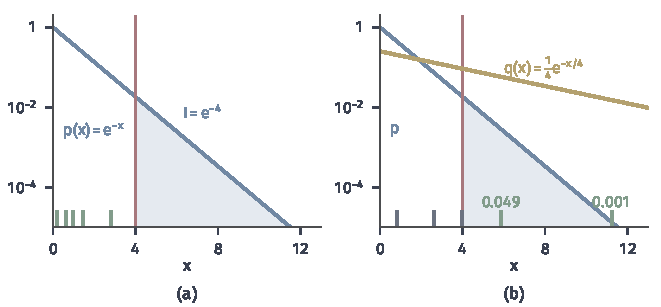
\includegraphics[width=112mm]{figures/07-probability/08-sampling-and-integration/matplotlib/vr-is-tail/figure.pdf}
 \caption{尾概率$I=\mathbb{P}(X>4)$的两种抽样，纵轴为对数刻度。蓝线为目标密度$p(x)=\mathrm{e}^{-x}$，浅蓝区域是$x>4$的尾部，红线是阈值。(a)用$u=0.37,0.81,0.06,0.52,0.23$按$x=-\ln u$生成的五个样本（绿色短线），全部落在阈值左侧。(b)同一组$u$按$x=-4\ln u$从黄线所示的$q$生成；越过阈值的两个样本为绿色并标出权重$w=4\mathrm{e}^{-3x/4}$，其余为灰色。}
 \label{fig:vr-is-tail}
\end{BookInlineFigure}

图~\ref{fig:vr-is-tail}对比了两种抽样。要算这一估计的方差，按式~\eqref{eq:vr-is-second-moment}在尾部积分：
\[
 M(q)=\int_4^{\infty}\frac{\mathrm{e}^{-2x}}{\tfrac14\mathrm{e}^{-x/4}}\,\mathrm{d}x=4\int_4^{\infty}\mathrm{e}^{-7x/4}\,\mathrm{d}x=\frac{16}{7}\mathrm{e}^{-7}\approx0.002084 .
\]
减去$I^2\approx0.000335$，单样本方差约为$0.001749$，只有直接平均的$0.01798$的$1/10.3$。这正是第~\ref{sec:vr-comparison}节例子中用到的数值。

\paragraph{覆盖条件去掉会怎样}
若建议分布只在$(0,6)$上有正密度，例如把$\operatorname{Exp}(1/4)$截断在$6$以内，$x>6$这部分尾部永远抽不到。重复定理的证明，估计的期望变为
\[
 \int_{\{q>0\}}f p\,\mathrm{d}\mu=\int_4^{6}\mathrm{e}^{-x}\,\mathrm{d}x=\mathrm{e}^{-4}-\mathrm{e}^{-6}\approx0.01584 ,
\]
比$I$少了$\mathrm{e}^{-6}/\mathrm{e}^{-4}\approx13.5\%$。这一偏差不随$n$减小，样本再多也只是越来越准地算出一个错误的数。

\paragraph{无偏而方差无穷}
仍对同一尾概率，改取$Q=\operatorname{Exp}(\lambda)$。对一般的$\lambda>0$，
\[
 M(q)=\int_4^{\infty}\frac{\mathrm{e}^{-2x}}{\lambda\mathrm{e}^{-\lambda x}}\,\mathrm{d}x=\frac1\lambda\int_4^{\infty}\mathrm{e}^{-(2-\lambda)x}\,\mathrm{d}x .
\]
$\lambda<2$时积分有限；$\lambda\geq2$时被积函数不衰减，$M(q)=\infty$。覆盖条件对每个$\lambda$都成立，所以估计都无偏、都收敛；但$\lambda\geq2$时方差为无穷。

$\lambda=2.5$时问题看得很清楚。建议样本进入尾部的概率只有$\mathrm{e}^{-10}\approx4.5\times10^{-5}$，而一旦进入，权重$w=0.4\mathrm{e}^{1.5x}$至少是$0.4\mathrm{e}^{6}\approx161$。估计值大部分时间是零，偶尔被一个巨大的权重拉高。图~\ref{fig:vr-is-running-mean}比较了两种$\lambda$下的运行平均：$\lambda=1/4$的三条路径平稳地收拢到真值；$\lambda=2.5$的三条路径在$n=2\times10^{5}$时分别只有$8$、$9$、$16$个尾部样本，终值为真值的$0.85$、$0.67$、$1.41$倍，路径呈台阶状跳动。

\begin{BookInlineFigure}
 \centering
 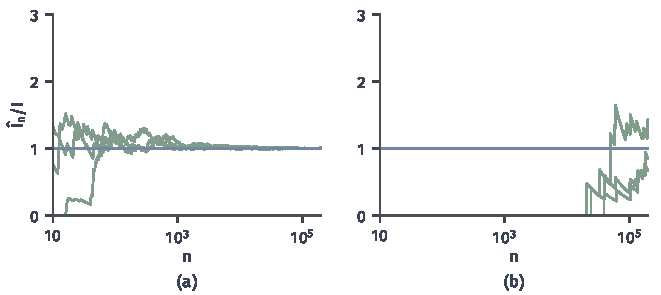
\includegraphics[width=112mm]{figures/07-probability/08-sampling-and-integration/matplotlib/vr-is-running-mean/figure.pdf}
 \caption{重要性采样估计的运行平均除以真值$I=\mathrm{e}^{-4}$，横轴为样本数（对数刻度），每图三条路径（种子11、12、13）。(a)$Q=\operatorname{Exp}(1/4)$，加权变量方差有限；(b)$Q=\operatorname{Exp}(2.5)$，估计仍无偏但加权变量的二阶矩为无穷。蓝线标出比值$1$。}
 \label{fig:vr-is-running-mean}
\end{BookInlineFigure}

\subsection{建议分布的选择}
\label{sec:vr-proposal-choice}

上一小节说明，权重公式正确只保证无偏；估计好不好，取决于式~\eqref{eq:vr-is-second-moment}的二阶矩$M(q)$。选择建议分布分两步。先从$M(q)$出发问：什么样的$q$最好？答案通常无法直接使用，于是再问：怎样用一次试运行拟合出一个可用的$q$，并且不破坏正式估计的性质？

\subsubsection{理想建议分布}
\label{sec:vr-ideal-proposal}

单样本方差是$M(q)-I^2$，其中$I$与$q$无关，所以比较建议分布就是比较$M(q)$。式~\eqref{eq:vr-is-second-moment}的被积函数是$f^2p^2/q$：分子大的地方，$q$也必须大，否则这一项会被放大。分子由$\lvert f\rvert p$决定，它衡量的是每个位置对积分的贡献，而不是样本在$P$下出现的频繁程度。

\begin{theorem}[理想建议分布]
\label{thm:vr-ideal-proposal}
设$0<\mathbb{E}_P[\lvert f(X)\rvert]<\infty$。对每个满足覆盖条件的密度$q$，
\begin{equation}
 M(q)\geq\bigl(\mathbb{E}_P[\lvert f(X)\rvert]\bigr)^2 ,
 \label{eq:vr-is-lower-bound}
\end{equation}
等号当且仅当$q$与
\begin{equation}
 q^{*}(x)=\frac{\lvert f(x)\rvert\,p(x)}{\mathbb{E}_P[\lvert f(X)\rvert]}
 \label{eq:vr-ideal-proposal}
\end{equation}
$\mu$几乎处处相等时成立。
\end{theorem}

\begin{proof}
记$S=\{q>0\}$，$a=\mathbb{E}_P[\lvert f\rvert]$。由覆盖条件，$a=\int_S\lvert f\rvert p\,\mathrm{d}\mu$。把被积函数拆成两个因子，用Cauchy--Schwarz不等式：
\[
 a=\int_S\frac{\lvert f\rvert p}{\sqrt{q}}\cdot\sqrt{q}\,\mathrm{d}\mu\leq\Bigl(\int_S\frac{f^2p^2}{q}\,\mathrm{d}\mu\Bigr)^{1/2}\Bigl(\int_S q\,\mathrm{d}\mu\Bigr)^{1/2} .
\]
右边第二个因子是$1$，第一个因子是$M(q)^{1/2}$，平方即得式~\eqref{eq:vr-is-lower-bound}。

等号成立当且仅当两个因子在$S$上几乎处处成比例，即存在常数$k$使$\lvert f\rvert p=k\,q$在$S$上几乎处处成立。两边在$S$上积分，得$k=a$，所以$q=\lvert f\rvert p/a$在$S$上几乎处处成立。在$S$之外$q=0$，而由覆盖条件$\lvert f\rvert p$也几乎处处为零。所以$q=q^{*}$几乎处处成立。反过来，$q=q^{*}$时直接计算得$M(q^{*})=a^2$。
\end{proof}

最小的单样本方差是$a^2-I^2$。$f$在$P$下几乎必然不变号时$\lvert I\rvert=a$，最小方差为零：每个样本的$f w$恰好等于$I$。$f$变号时$a>\lvert I\rvert$，即使用理想建议，方差也不为零。

\paragraph{尾概率：零方差与循环}
尾概率中$f=\mathbf{1}_{\{x>4\}}$不变号，$a=I=\mathrm{e}^{-4}$，理想建议是
\[
 q^{*}(x)=\frac{\mathrm{e}^{-x}\mathbf{1}_{\{x>4\}}}{\mathrm{e}^{-4}}=\mathrm{e}^{-(x-4)}\mathbf{1}_{\{x>4\}} ,
\]
也就是在$X>4$条件下$X$的分布。按它抽样，每个样本都落在尾部，权重是常数：
\[
 w(x)=\frac{\mathrm{e}^{-x}}{\mathrm{e}^{-(x-4)}}=\mathrm{e}^{-4},\qquad x>4 .
\]
一个样本就给出精确的$I$。问题在于$q^{*}$的归一化常数正是$a=I$：写出$q^{*}$，等于已经知道了答案。这里能写出来，只是因为指数分布的尾部恰好还是指数分布。一般地，理想建议告诉我们抽样应当往哪里集中，而不是一个可以直接使用的分布。

\paragraph{变号的被积函数}
取$P=\mathcal{N}(0,1)$，$f(x)=x$，$I=0$。此时$a=\mathbb{E}\lvert X\rvert=\sqrt{2/\pi}$，理想建议
\[
 q^{*}(x)=\frac{\lvert x\rvert\varphi(x)}{\sqrt{2/\pi}}
\]
在原点处为零、在$\pm1$附近各有一个峰。它的单样本方差是
\[
 a^2-I^2=\frac{2}{\pi}\approx0.637 ,
\]
比直接平均的$\operatorname{Var}(X)=1$小，但不为零：正负两部分的样本各自带着符号，平均时仍有波动。若把$f$拆成正部$f^{+}=\max\{f,0\}$与负部$f^{-}=\max\{-f,0\}$，分别用各自的理想建议计算再相减，两部分都是零方差。图~\ref{fig:vr-ideal-proposal}画出两个例子中的$p$、贡献$\lvert f\rvert p$与$q^{*}$。

\begin{BookInlineFigure}
 \centering
 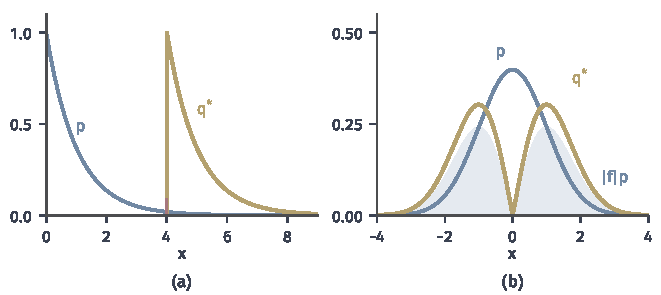
\includegraphics[width=112mm]{figures/07-probability/08-sampling-and-integration/matplotlib/vr-ideal-proposal/figure.pdf}
 \caption{理想建议分布$q^{*}=\lvert f\rvert p/\mathbb{E}_P\lvert f\rvert$（黄线）与目标密度$p$（蓝线）。(a)$p(x)=\mathrm{e}^{-x}$，$f=\mathbf{1}_{\{x>4\}}$：$q^{*}$是平移到$4$的指数密度，贡献$\lvert f\rvert p$为$x>4$下方面积$\mathrm{e}^{-4}$，在此刻度下几乎看不见。(b)$p=\mathcal{N}(0,1)$，$f(x)=x$：浅蓝区域为$\lvert x\rvert\varphi(x)$，$q^{*}$是它除以$\sqrt{2/\pi}$，在原点为零。}
 \label{fig:vr-ideal-proposal}
\end{BookInlineFigure}

\paragraph{在分布族内选择}
既然$q^{*}$通常不可用，退一步在一个可采样的族中找使$M(q)$最小的成员。尾概率中取$Q=\operatorname{Exp}(\lambda)$，上一小节已经算出，$0<\lambda<2$时
\begin{equation}
 v(\lambda)=M(q_\lambda)-I^2=\frac{\mathrm{e}^{-4(2-\lambda)}}{\lambda(2-\lambda)}-\mathrm{e}^{-8} .
 \label{eq:vr-exp-family-variance}
\end{equation}
对第一项取对数，得到$4\lambda-8-\ln\lambda-\ln(2-\lambda)$，令它的导数为零：
\[
 4-\frac1\lambda+\frac{1}{2-\lambda}=0 .
\]
两边乘$\lambda(2-\lambda)$整理，得
\[
 4\lambda^2-10\lambda+2=0 .
\]
在$(0,2)$内的根是$\lambda^{*}=(5-\sqrt{17})/4\approx0.219$，此时$v(\lambda^{*})\approx0.001730$，比直接平均小$10.4$倍。$\lambda^{*}$对应的平均值$1/\lambda^{*}\approx4.56$略大于阈值$4$：抽样集中在尾部的起点附近，那里正是$\lvert f\rvert p$最大的地方。

\begin{BookInlineFigure}
 \centering
 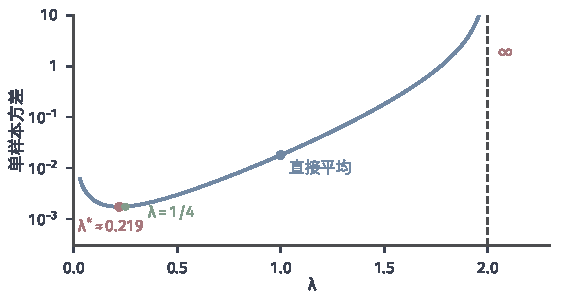
\includegraphics[width=96mm]{figures/07-probability/08-sampling-and-integration/matplotlib/vr-is-second-moment/figure.pdf}
 \caption{尾概率$\mathbb{P}(X>4)$用$Q=\operatorname{Exp}(\lambda)$作建议时的单样本方差$v(\lambda)$，纵轴为对数刻度。蓝点$\lambda=1$即直接平均，红点为最优$\lambda^{*}\approx0.219$，绿点为正文例子用的$\lambda=1/4$；虚线$\lambda=2$右侧方差为无穷。}
 \label{fig:vr-is-second-moment}
\end{BookInlineFigure}

图~\ref{fig:vr-is-second-moment}画出$v(\lambda)$。曲线有两个陡峭的方向。$\lambda\to0$时建议分布摊得过宽，大部分样本落在远离阈值、贡献极小的地方；$\lambda\to2$时建议分布的尾部衰减得和$p^2$一样快，权重平方在远处不再衰减，二阶矩发散。后一种情形是更危险的一侧：它不表现为估计变差一点，而是方差直接变为无穷。

\paragraph{尾部过轻}
这个现象有一般的形式。$f$有界时，$M(q)\leq\sup\lvert f\rvert^2\,\mathbb{E}_P[w]$，若$q$的尾部至少和$p$一样重，使$w=p/q$有界，则$M(q)$有限。反之，若在某个方向上$q$比$p$衰减得快很多，$w$在那里无界，$f^2p^2/q$可能不可积。所以选建议分布时，宁可尾部偏重，不可偏轻。

\subsubsection{试运行中的拟合}
\label{sec:vr-pilot-fitting}

当理想建议无法直接写出时，可以先用一个覆盖面足够宽的分布$q_0$做一次试运行，从试运行样本中看出贡献集中在哪里，再从一个可采样、密度可计算的族中挑出与$q^{*}$相近的成员。

\paragraph{主要思想}
设$Y_1,\dots,Y_m$独立且都服从$q_0$，$q_0$覆盖$fp$。记
\begin{equation}
 c_j=\frac{\lvert f(Y_j)\rvert\,p(Y_j)}{q_0(Y_j)},\qquad j=1,\dots,m .
 \label{eq:vr-pilot-contribution}
\end{equation}
由换测度恒等式，对任意使积分存在的函数$g$，
\[
 \mathbb{E}_{q_0}\bigl[c\,g(Y)\bigr]=\int\lvert f\rvert p\,g\,\mathrm{d}\mu=a\,\mathbb{E}_{q^{*}}[g] .
\]
所以以$c_j$为权重的加权平均$\sum_j c_jg(Y_j)/\sum_j c_j$近似$\mathbb{E}_{q^{*}}[g]$：带权重$c_j$的试运行样本是$q^{*}$的一个粗略画像，$c_j$可以看成第$j$个试运行点对积分的贡献。

拟合时在族中挑出各项矩与这个画像一致的成员。以方差为$1$的正态位置族$\mathcal{N}(m,1)$为例，与$q^{*}$的KL散度为
\[
 D_{\mathrm{KL}}\bigl(q^{*}\Vert\mathcal{N}(m,1)\bigr)=\int q^{*}\ln q^{*}\,\mathrm{d}x+\frac12\ln(2\pi)+\frac12\mathbb{E}_{q^{*}}\bigl[(X-m)^2\bigr] .
\]
只有最后一项依赖$m$，它在$m=\mathbb{E}_{q^{*}}[X]$时最小。把$\mathbb{E}_{q^{*}}[X]$换成加权平均，就得到以贡献为权重的均值。用KL散度逼近一个分布的一般讨论见第~\ref{chap:distribution-approximation}章。

贡献集中在几个分离的区域时，每个区域配一个成分，成分的权重取该区域贡献所占的比例。再留一份$q_0$本身作为\term{防御性混合}（defensive mixture）成分：
\begin{equation}
 q=\alpha\,q_0+(1-\alpha)\sum_{k=1}^{K}\pi_k\,\mathcal{N}(m_k,1),\qquad 0<\alpha<1 .
 \label{eq:vr-defensive-mixture}
\end{equation}
这一份保证了$q\geq\alpha q_0$，于是$w=p/q\leq p/(\alpha q_0)$：只要$p/q_0$有界，权重就有界，拟合得再差，二阶矩也不会发散；试运行没有看到的区域，也仍以$\alpha q_0$的密度被抽到。

\paragraph{计算过程}
下面结合一个两区域的例子写出计算过程。目标$P=\mathcal{N}(0,1)$，
\[
 f(x)=\mathbf{1}_{\{x<-2.5\}}+\mathbf{1}_{\{x>3\}} ,
\]
真值$I=\Phi(-2.5)+1-\Phi(3)=0.006210+0.001350=0.007560$，左侧贡献占$82\%$。直接平均的单样本方差为$I(1-I)\approx0.007502$。

\needspace{6\baselineskip}
\paragraph{变量}
\begin{itemize}
 \item 试运行分布$q_0$与试运行样本$Y_1,\dots,Y_m$；例中$q_0=\mathcal{N}(0,3^2)$，$m=30$。
 \item 贡献$c_j$，按式~\eqref{eq:vr-pilot-contribution}计算，长度为$m$的非负数组。
 \item 区域划分及区域数$K$；例中按符号分为左右两区，$K=2$。
 \item 拟合参数：成分权重$\pi_k$与成分均值$m_k$，$k=1,\dots,K$；防御比例$\alpha$，例中$\alpha=0.2$。
\end{itemize}

\needspace{6\baselineskip}
\paragraph{步骤}
\begin{enumerate}
 \item \textbf{试运行。}抽取$Y_1,\dots,Y_m\sim q_0$，计算各$c_j$。例中（种子3）$30$个点里有$9$个落进贡献区，其中只有$4$个的贡献不可忽略：
 \[
 \begin{array}{lcccc}
  y_j & -3.165 & -2.596 & 3.007 & 4.637\\
  c_j & 0.03492 & 0.15020 & 0.05394 & 0.00021
 \end{array}
 \]
 另外$5$个点落在$\lvert y\rvert>5.8$处，那里$p$极小，贡献都小于$10^{-6}$。

 \item \textbf{按区域汇总。}对每个区域$k$计算贡献之和$s_k$。例中
 \[
  s_1=0.03492+0.15020=0.18512,\qquad s_2=0.05394+0.00021=0.05415 .
 \]

 \item \textbf{成分权重。}取$\pi_k=s_k/\sum_l s_l$。例中
 \[
  \pi_1=\frac{0.18512}{0.23927}=0.774,\qquad \pi_2=0.226 .
 \]
 真实比例是$0.821$与$0.179$，三十个试运行点给出的估计已经大致正确。

 \item \textbf{成分均值。}取$m_k=\sum_{j\in k}c_jy_j/s_k$。例中
 \[
  m_1=\frac{0.03492\times(-3.165)+0.15020\times(-2.596)}{0.18512}=-2.703 ,
 \]
 同样算得$m_2=3.013$。

 \item \textbf{组装建议。}代入式~\eqref{eq:vr-defensive-mixture}。例中
 \[
  q=0.2\,\mathcal{N}(0,3^2)+0.8\bigl[0.774\,\mathcal{N}(-2.703,1)+0.226\,\mathcal{N}(3.013,1)\bigr] .
 \]
\end{enumerate}
最终得到的$q$由数值积分算得单样本方差$M(q)-I^2\approx1.99\times10^{-4}$，是直接平均的$1/37.7$。这里$p/q_0=3\mathrm{e}^{-4x^2/9}\leq3$，所以权重不超过$3/\alpha=15$。图~\ref{fig:vr-mixture-fit}左图是试运行点及其贡献，右图把拟合的$q$与$q^{*}$放在一起。

\begin{BookInlineFigure}
 \centering
 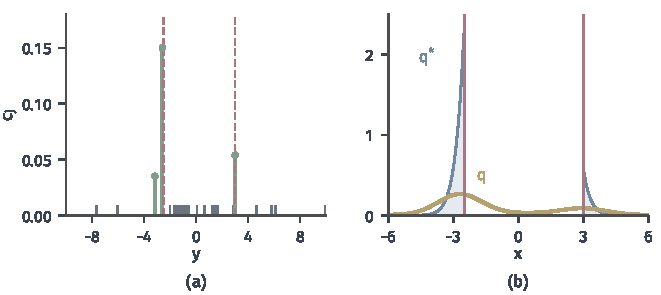
\includegraphics[width=112mm]{figures/07-probability/08-sampling-and-integration/matplotlib/vr-mixture-fit/figure.pdf}
 \caption{两区域贡献的建议拟合，$P=\mathcal{N}(0,1)$，$f=\mathbf{1}_{\{x<-2.5\}}+\mathbf{1}_{\{x>3\}}$，红色虚线或实线为两个阈值。(a)$q_0=\mathcal{N}(0,3^2)$的$30$个试运行点（种子3）：灰色短线为贡献可忽略的点，绿色竖线高度为贡献$c_j$。(b)蓝线与浅蓝区域为理想建议$q^{*}=fp/I$，黄线为拟合的防御性混合$q$。}
 \label{fig:vr-mixture-fit}
\end{BookInlineFigure}

\paragraph{没看到不等于没有}
试运行的范围不够时，拟合会漏掉区域。把试运行分布换成较窄的$q_0=\mathcal{N}(0,1.5^2)$，同样抽$30$个点（种子0），只有一个点$-3.488$落进左区，没有点越过$3$。按上面的步骤只能拟合出左侧一个成分$\mathcal{N}(-3.488,1)$。若不留防御成分，右区$x>3$只能靠这个远在左边的成分偶尔覆盖，单样本方差约为$1.3\times10^{5}$，是直接平均的$1.8\times10^{7}$倍；留下$\alpha=0.2$的$q_0$后，方差降为约$7.4\times10^{-4}$，仍比直接平均好约$10$倍。试运行中某个区域一个点也没有，只说明$m$个点没有落到那里，不说明那里对积分没有贡献。

\subsubsection{固定建议后的估计}
\label{sec:vr-fixed-proposal}

拟合出的$q$依赖试运行样本，本身是随机的。正式估计必须说明：在$q$随机的情况下，加权平均还是否无偏、方差怎样计算。

把试运行的全部结果记为$D=(Y_1,\dots,Y_m)$，拟合的建议记为$q_D$。正式计算在给定$D$后，用一组与$D$独立的新随机数抽取$X_1,\dots,X_n\sim q_D$，再计算
\[
 \hat{I}_n^{\mathrm{IS}}=\frac1n\sum_{i=1}^{n}f(X_i)\frac{p(X_i)}{q_D(X_i)} .
\]
图~\ref{fig:vr-two-stage}画出这一两阶段结构。

\begin{BookInlineFigure}
 \centering
 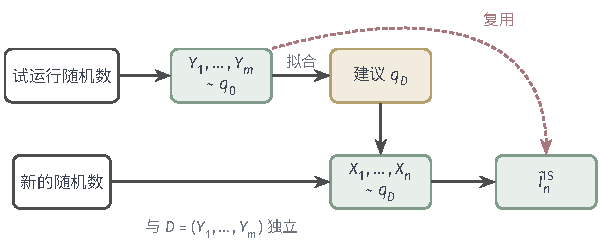
\includegraphics[width=102mm]{figures/07-probability/08-sampling-and-integration/tikz/vr-two-stage/figure.pdf}
 \caption{两阶段重要性采样。试运行随机数产生$D=(Y_1,\dots,Y_m)$并拟合建议$q_D$；正式样本由与$D$独立的新随机数按$q_D$生成。红色虚线表示把试运行点直接混入正式估计，这样做会破坏下面的条件无偏性。}
 \label{fig:vr-two-stage}
\end{BookInlineFigure}

\begin{theorem}[两阶段估计的无偏性]
\label{thm:vr-two-stage}
设$\mathbb{E}_P[\lvert f\rvert]<\infty$，对几乎每个试运行结果$D$，$q_D$都覆盖$fp$，且正式样本所用的随机数与$D$独立。则
\begin{equation}
 \mathbb{E}\bigl[\hat{I}_n^{\mathrm{IS}}\bigm|D\bigr]=I,\qquad \mathbb{E}\bigl[\hat{I}_n^{\mathrm{IS}}\bigr]=I .
 \label{eq:vr-two-stage-unbiased}
\end{equation}
若再有$\mathbb{E}[M(q_D)]<\infty$，则
\begin{equation}
 \operatorname{Var}\bigl(\hat{I}_n^{\mathrm{IS}}\bigr)=\frac{\mathbb{E}[M(q_D)]-I^2}{n} .
 \label{eq:vr-two-stage-variance}
\end{equation}
\end{theorem}

\begin{proof}
正式样本可以写成$X_i=T(D,\bm{U}_i)$，其中$\bm{U}_1,\dots,\bm{U}_n$与$D$独立，且对固定的$d$，$T(d,\bm{U}_i)$服从$q_d$。由第~\ref{chap:conditional-distributions}章，$\bm{U}_i$与$D$独立时，给定$D=d$的条件期望可以把$d$代入后只对$\bm{U}_i$求期望。对固定的$d$，这是建议$q_d$下的普通重要性采样，由定理~\ref{thm:vr-change-of-measure}，它的期望是$I$。这就是式~\eqref{eq:vr-two-stage-unbiased}的第一式；再用全期望公式得到第二式。

同样，给定$D=d$时的条件方差是$(M(q_d)-I^2)/n$。由全方差公式，总方差等于条件方差的期望加条件期望的方差；条件期望恒为$I$，后一项为零，于是得到式~\eqref{eq:vr-two-stage-variance}。
\end{proof}

定理中两个条件的作用不同。“对每个$D$都覆盖”保证无论试运行结果如何，正式估计都不偏；防御性混合使这一条自动成立，因为$q_D\geq\alpha q_0$而$q_0$覆盖$fp$。“新随机数与$D$独立”保证条件化以后正式样本确实服从$q_D$。在固定$D$下，正式样本的$f w$值独立同分布，用它们的样本方差除以$n$就可以估计条件方差。

\paragraph{复用试运行点}
如果把试运行点$Y_j$也代入同一个加权公式，即在正式平均中加入$f(Y_j)p(Y_j)/q_D(Y_j)$，问题出在两处：$Y_j$并不服从$q_D$，而是服从$q_0$；$q_D$又是由$Y_j$拟合出来的，在$Y_j$附近往往偏大。这一项的期望一般不等于$I$。试运行点可以利用，但要用它实际来源的密度：$f$非负时，$\sum_jc_j/m$就是基于$q_0$的一个无偏估计，例中为$0.00798$。正式估计在给定$D$时的条件期望恒为$I$，所以两者不相关，可以按固定的比例合并。

\paragraph{混合形式不保证有限方差}
式~\eqref{eq:vr-two-stage-variance}要求$\mathbb{E}[M(q_D)]<\infty$，这要对试运行的每种可能结果检查。混合本身不能保证这一点。仍用上面的两区域例子，如果在步骤4中同时用加权方差拟合每个成分的方差，左右两个成分的标准差分别只有$0.223$与$0.103$。没有防御成分时，$q$在远处按$\mathrm{e}^{-x^2/(2\times0.223^2)}$衰减，比$p^2\propto\mathrm{e}^{-x^2}$快得多，左区上$p^2/q$不可积，$M(q)=\infty$。加上$\alpha=0.2$的$q_0=\mathcal{N}(0,3^2)$后，权重有界，单样本方差约为$7.7\times10^{-5}$。起作用的是一个尾部足够重的成分，而不是混合这一形式。

试运行越长，拟合越可靠，但它的成本也计入总预算。试运行与正式计算之间怎样分配预算，由第~\ref{chap:sampling-budget-method-selection}章讨论。

\subsection{自归一化估计}
\label{sec:vr-self-normalized}

许多目标分布只知道到一个常数倍：能算$\widetilde{p}(x)\geq0$，而$p=\widetilde{p}/Z$中的归一化常数
\[
 Z=\int\widetilde{p}\,\mathrm{d}\mu,\qquad 0<Z<\infty
\]
无法直接计算。第~\ref{chap:sample-generation}章的拒绝采样与Metropolis--Hastings采样都只用到$\widetilde{p}$。这时权重$p/q$算不出来，只能算$\widetilde{w}=\widetilde{p}/q=Zw$。

办法是用同一批样本同时估计$Z$。由换测度恒等式，$\mathbb{E}_Q[\widetilde{w}]=Z$，$\mathbb{E}_Q[\widetilde{w}f]=ZI$，两者相除，未知的$Z$约去。

\begin{definition}[自归一化估计]
\label{def:vr-self-normalized}
设$q$覆盖整个目标，即$\{\widetilde{p}>0\}\subseteq\{q>0\}$。对独立且都服从$Q$的$X_1,\dots,X_n$，记$\widetilde{w}_i=\widetilde{p}(X_i)/q(X_i)$，称
\begin{equation}
 \hat{I}_n^{\mathrm{SN}}=\frac{\sum_{i=1}^{n}\widetilde{w}_i\,f(X_i)}{\sum_{i=1}^{n}\widetilde{w}_i}
 \label{eq:vr-self-normalized}
\end{equation}
为\term{自归一化重要性采样}（self-normalized importance sampling）估计；分母为零时规定估计值为$0$。
\end{definition}

覆盖的要求比定义~\ref{def:vr-importance-sampling}更强：分母要估计整个$Z$，所以凡是$\widetilde{p}>0$的地方都要覆盖，不能只覆盖$f\widetilde{p}\neq0$的部分。

\begin{theorem}[自归一化估计的一致性]
\label{thm:vr-sn-consistency}
设$q$覆盖整个目标且$\mathbb{E}_P[\lvert f\rvert]<\infty$。则$\hat{I}_n^{\mathrm{SN}}\xrightarrow{\mathrm{a.s.}}I$。
\end{theorem}

\begin{proof}
由换测度恒等式，$\widetilde{w}$与$\widetilde{w}f$在$Q$下可积，期望分别是$Z$与$ZI$。由强大数律，几乎必然有
\[
 \frac1n\sum_{i=1}^{n}\widetilde{w}_i\to Z,\qquad \frac1n\sum_{i=1}^{n}\widetilde{w}_if(X_i)\to ZI .
\]
因为$Z>0$，在这些样本点上分母从某个$n$起为正，比值收敛到$ZI/Z=I$。
\end{proof}

\paragraph{有限样本的偏差}
比值的期望一般不是期望的比值。最极端的情形是$n=1$：只要$\widetilde{w}_1>0$，式~\eqref{eq:vr-self-normalized}就等于$f(X_1)$，于是估计的期望是$f$在$Q$下（限制在$\widetilde{w}>0$上）的平均，而不是在$P$下的平均。另一种有限样本现象是分母为零：若$\widetilde{p}$在$q$的支撑上有一部分为零，所有样本都可能落在那里，这时估计没有信息。

用一个能手算的例子看这些量。目标$\widetilde{p}(x)=x^2\mathrm{e}^{-x}$（$x>0$），它是$\operatorname{Gamma}(3,1)$的未归一化密度，$Z=2$；要算$I=\mathbb{E}_P[X]=3$。建议$Q=\operatorname{Exp}(1/2)$，于是
\[
 q(x)=\tfrac12\mathrm{e}^{-x/2},\qquad \widetilde{w}(x)=2x^2\mathrm{e}^{-x/2} .
\]
$n=1$时估计的期望是$\mathbb{E}_Q[X]=2$，偏差为$-1$。仍用前面那五个均匀数，按$x=-2\ln u$生成五个建议样本：
\[
 x=1.989,\quad 0.421,\quad 5.627,\quad 1.308,\quad 2.939 .
\]
对应的权重为
\[
 \widetilde{w}=2.926,\quad 0.288,\quad 3.799,\quad 1.779,\quad 3.974 .
\]
权重和为$12.766$，加权和$\sum\widetilde{w}_ix_i=41.326$，于是
\[
 \hat{I}_5^{\mathrm{SN}}=\frac{41.326}{12.766}=3.237 .
\]
副产品是$Z$的无偏估计$12.766/5=2.553$。

\paragraph{渐近误差}
把误差写成
\[
 \hat{I}_n^{\mathrm{SN}}-I=\frac{\frac1n\sum_{i=1}^{n}\widetilde{w}_i\bigl(f(X_i)-I\bigr)}{\frac1n\sum_{i=1}^{n}\widetilde{w}_i} .
\]
分子是独立同分布变量$\widetilde{w}(f-I)$的平均，它的期望是$ZI-IZ=0$。若中心化加权量的二阶矩
\begin{equation}
 \tau^2=\mathbb{E}_Q\bigl[\widetilde{w}(X)^2\bigl(f(X)-I\bigr)^2\bigr]<\infty ,
 \label{eq:vr-sn-tau}
\end{equation}

由第~\ref{chap:central-limit-theorem}章的中心极限定理，分子乘以$\sqrt{n}$依分布收敛到$\mathcal{N}(0,\tau^2)$；分母几乎必然收敛到$Z$。由第~\ref{chap:weak-convergence-of-distributions}章的Slutsky定理，
\begin{equation}
 \sqrt{n}\,\bigl(\hat{I}_n^{\mathrm{SN}}-I\bigr)\xrightarrow{\mathrm{d}}\mathcal{N}\Bigl(0,\frac{\tau^2}{Z^2}\Bigr) .
 \label{eq:vr-sn-clt}
\end{equation}
要检查的是$\widetilde{w}(f-I)$的二阶矩，而不是$\widetilde{w}f$的二阶矩：减去$I$以后，大权重落在$f\approx I$处的样本不再放大误差。式~\eqref{eq:vr-sn-clt}是渐近结论，它不给出任何固定$n$下的覆盖保证。

把分母写成$Z(1+\delta)$，$\delta$是分母的相对误差，展开$1/(1+\delta)\approx1-\delta$并取期望，可以得到偏差的主项：
\begin{equation}
 \mathbb{E}\bigl[\hat{I}_n^{\mathrm{SN}}\bigr]-I\approx-\frac{\mathbb{E}_Q\bigl[\widetilde{w}^2(f-I)\bigr]}{nZ^2} .
 \label{eq:vr-sn-bias}
\end{equation}
它是分子与分母协方差的结果。这只是主项：严格化需要控制分母接近零的事件以及展开的余项。例中数值积分给出$\tau^2/Z^2\approx3.687$，偏差系数$\approx-0.527$。偏差的平方与$1/n^2$同阶，方差与$1/n$同阶，样本量大时偏差可以忽略。图~\ref{fig:vr-snis}(a)用$4\times10^{4}$次独立重复验证了这两个阶：$n\geq8$时偏差与$0.527/n$吻合，$n=2$时偏差约为$0.48$，主项公式在这样小的样本下并不准确。顺便比较，直接从$\operatorname{Gamma}(3,1)$抽样时单样本方差是$3$，这里的渐近方差$3.687$稍大。

\begin{BookInlineFigure}
 \centering
 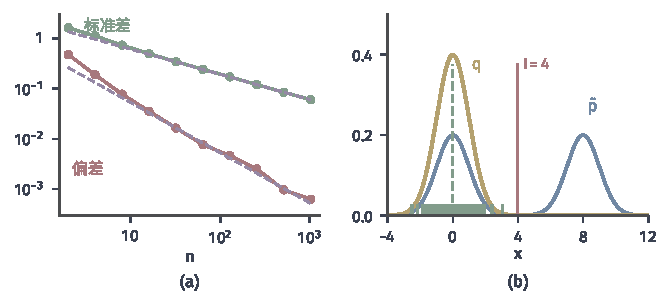
\includegraphics[width=112mm]{figures/07-probability/08-sampling-and-integration/matplotlib/vr-snis/figure.pdf}
 \caption{自归一化估计的偏差与覆盖问题。(a)目标$\operatorname{Gamma}(3,1)$，$f(x)=x$，建议$\operatorname{Exp}(1/2)$；每个$n$独立重复$4\times10^{4}$次（种子5），绿线为估计的标准差，红线为偏差的绝对值，紫色虚线为渐近参照$\sqrt{3.687/n}$与$0.527/n$。(b)目标$\widetilde{p}=\tfrac12\varphi(x)+\tfrac12\varphi(x-8)$（蓝线），建议$\mathcal{N}(0,1)$（黄线）；绿色短线为前$200$个建议样本，绿色虚线为$n=1000$时的估计值，红线为真值$4$。}
 \label{fig:vr-snis}
\end{BookInlineFigure}

\paragraph{权重的有效样本量看不到漏掉的区域}
实践中常用权重计算
\[
 n_{\mathrm{w}}=\frac{\bigl(\sum_{i=1}^{n}\widetilde{w}_i\bigr)^2}{\sum_{i=1}^{n}\widetilde{w}_i^2} .
\]
它介于$1$与$n$之间：权重全相等时为$n$，一个权重压倒其余时接近$1$。上面的五点例子中$n_{\mathrm{w}}=3.88$。它衡量的是已经抽到的样本之间权重的分散程度，看不到没有抽到的地方。

图~\ref{fig:vr-snis}(b)是一个反例。目标是两个相距$8$的正态峰的等权混合，真值$\mathbb{E}_P[X]=4$；建议$\mathcal{N}(0,1)$只盖住左峰。覆盖条件成立（$q$处处为正），所以定理~\ref{thm:vr-sn-consistency}保证估计最终收敛到$4$。但权重
\[
 \widetilde{w}(x)=\tfrac12+\tfrac12\mathrm{e}^{8x-32}
\]
只在$x>4$附近才明显偏离$\tfrac12$，而建议样本进入那里的概率约为$3\times10^{-5}$。$n=1000$（种子6）时，估计值为$-0.012$，而$n_{\mathrm{w}}=1000.0$：所有权重几乎相同，指标显示“完美”，估计却错了整整一个峰。经验指标稳定不能证明建议分布覆盖了目标的重要区域。


\section{改变计算公式}
\label{sec:vr-change-formula}

上一节保持被平均的对象不变，改变样本从哪里来。本节反过来：样本仍按$P$抽取，但不再直接平均$f(X)$，而是平均另一个期望同为$I$、波动更小的量。构造这样的量有两条路。一是找一个与$f$同步起伏、期望已知的辅助量，把可以预测的那部分波动减掉；二是把输入中的一部分随机性用条件平均精确地算掉，只对剩下的部分抽样。两种做法都会增加每个样本的计算，比较时要按第~\ref{sec:vr-comparison}节计入成本。

\subsection{控制变量}
\label{sec:vr-control-variates}

回到导言的第二个例子：
\[
 I=\int_0^1\mathrm{e}^{u}\,\mathrm{d}u=\mathrm{e}-1 .
\]
按$U\sim\operatorname{Unif}(0,1)$抽样，$\mathrm{e}^{U}$的方差为
\[
 \sigma^2=\mathbb{E}\bigl[\mathrm{e}^{2U}\bigr]-(\mathrm{e}-1)^2=\frac{\mathrm{e}^2-1}{2}-(\mathrm{e}-1)^2\approx0.2420 .
\]
这些波动的主要来源一目了然：$U$偏大，$\mathrm{e}^{U}$就偏大。而$U$本身的期望$1/2$是已知的。如果某次抽到的$U$比$1/2$大了$0.1$，就可以预先判断$\mathrm{e}^{U}$大约偏高了$0.1$乘以某个斜率，把这一部分减掉。

\begin{definition}[控制变量估计]
\label{def:vr-control-variate}
设$h$是一个在$P$下期望$\mu_h=\mathbb{E}_P[h(X)]$已知的函数，$\beta$为实数。对独立且都服从$P$的$X_1,\dots,X_n$，称
\begin{equation}
 \hat{I}_n^{\mathrm{CV}}(\beta)=\frac1n\sum_{i=1}^{n}\Bigl[f(X_i)-\beta\bigl(h(X_i)-\mu_h\bigr)\Bigr]
 \label{eq:vr-control-variate}
\end{equation}
为以$h$为\term{控制变量}（control variate）、系数为$\beta$的估计。
\end{definition}

减去的量期望为零，所以对任意固定的$\beta$，估计都无偏。要选的是使方差最小的$\beta$。

\begin{theorem}[控制变量的最优系数]
\label{thm:vr-control-variate}
设$\mathbb{E}_P[f^2]<\infty$，$\mathbb{E}_P[h^2]<\infty$，$\sigma_h^2=\operatorname{Var}_P(h)>0$，记$\sigma_f^2=\operatorname{Var}_P(f)$，$\gamma=\operatorname{Cov}_P(f,h)$。对固定的$\beta$，
\begin{equation}
 n\operatorname{Var}\bigl(\hat{I}_n^{\mathrm{CV}}(\beta)\bigr)=\sigma_f^2-2\beta\gamma+\beta^2\sigma_h^2 .
 \label{eq:vr-cv-variance}
\end{equation}
它在
\begin{equation}
 \beta^{*}=\frac{\gamma}{\sigma_h^2}
 \label{eq:vr-cv-beta}
\end{equation}
处取到最小值$\sigma_f^2(1-\rho^2)$，其中$\rho=\gamma/(\sigma_f\sigma_h)$是$f(X)$与$h(X)$的相关系数（$\sigma_f=0$时最小值为$0$）。
\end{theorem}

\begin{proof}
单项$f-\beta(h-\mu_h)$的方差由方差与协方差的双线性得到$\sigma_f^2-2\beta\gamma+\beta^2\sigma_h^2$，独立平均再除以$n$，这是式~\eqref{eq:vr-cv-variance}。对$\beta$配方：
\[
 \sigma_f^2-2\beta\gamma+\beta^2\sigma_h^2=\sigma_h^2\Bigl(\beta-\frac{\gamma}{\sigma_h^2}\Bigr)^2+\sigma_f^2-\frac{\gamma^2}{\sigma_h^2} .
\]
第一项非负，在$\beta=\beta^{*}$时为零。最小值$\sigma_f^2-\gamma^2/\sigma_h^2$在$\sigma_f>0$时写成$\sigma_f^2(1-\rho^2)$。
\end{proof}

\paragraph{这是一次投影}
把中心化的$f-I$与$h-\mu_h$看成平方可积随机变量空间中的两个向量，$\beta^{*}(h-\mu_h)$正是$f-I$在$h-\mu_h$方向上的正交投影，剩下的$f-I-\beta^{*}(h-\mu_h)$与$h$不相关。也可以说：用$h$对$f$作线性回归，$\beta^{*}$是回归斜率，控制变量估计平均的是回归残差加上$I$。$h$能解释$f$的方差比例为$\rho^2$，这部分被消去，只剩$1-\rho^2$。同时用$k$个控制变量$\bm{h}=(h_1,\dots,h_k)$时，若它们的协方差矩阵$\bm{\Sigma}_{\bm{h}}$可逆，同样配方可得最优系数向量$\bm{\Sigma}_{\bm{h}}^{-1}\operatorname{Cov}_P(\bm{h},f)$，即向$k$维子空间的投影。

\paragraph{例子的数值}
对$f(u)=\mathrm{e}^{u}$与$h(u)=u$，$\mu_h=1/2$，$\sigma_h^2=1/12$。由分部积分，
\[
 \mathbb{E}\bigl[U\mathrm{e}^{U}\bigr]=\int_0^1u\mathrm{e}^{u}\,\mathrm{d}u=\bigl[(u-1)\mathrm{e}^{u}\bigr]_0^1=1 .
\]
于是
\[
 \gamma=1-\frac{\mathrm{e}-1}{2}\approx0.14086,\qquad \beta^{*}=12\gamma\approx1.6903 .
\]
最小方差为
\[
 \sigma_f^2-\frac{\gamma^2}{\sigma_h^2}=0.24204-12\times0.14086^2\approx0.003940 ,
\]
$\rho^2\approx0.984$，方差降为原来的$1/61$。$h(U)=U$在抽样时已经得到，几乎不增加成本，相对效率约为$61$。

图~\ref{fig:vr-control-variate}(a)显示了抵消是怎样发生的：蓝色的$\mathrm{e}^{u}$在$[0,1]$上从$1$升到$2.72$，减去紫色直线$I+\beta^{*}(u-\tfrac12)$的倾斜部分后，绿色的被平均函数只在$1.65$到$1.88$之间变化。剩下的波动来自$\mathrm{e}^{u}$的弯曲，线性的$h$抵消不了它。图(b)是式~\eqref{eq:vr-cv-variance}作为$\beta$的函数：一条开口向上的抛物线，$\beta=0$是直接平均，$\beta^{*}$处取最小。

\begin{BookInlineFigure}
 \centering
 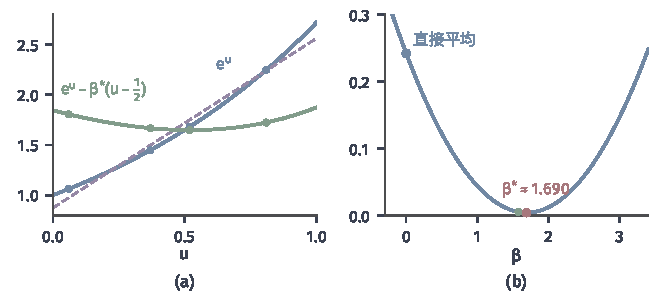
\includegraphics[width=112mm]{figures/07-probability/08-sampling-and-integration/matplotlib/vr-control-variate/figure.pdf}
 \caption{以$h(U)=U$为控制变量计算$\int_0^1\mathrm{e}^{u}\,\mathrm{d}u$。(a)蓝线为$\mathrm{e}^{u}$，紫色虚线为$I+\beta^{*}(u-\tfrac12)$，绿线为$\mathrm{e}^{u}-\beta^{*}(u-\tfrac12)$；圆点标出$u=0.37,0.81,0.06,0.52$处的值。(b)单样本方差$\sigma_f^2-2\beta\gamma+\beta^2/12$随$\beta$的变化：蓝点为直接平均，红点为$\beta^{*}$，绿点为由四个样本估计的$\hat{\beta}=1.577$。}
 \label{fig:vr-control-variate}
\end{BookInlineFigure}

\paragraph{系数由同一批样本估计}
实际中$\gamma$通常未知，$\beta^{*}$也就未知。最直接的办法是用同一批样本的样本协方差与样本方差估计它：
\begin{equation}
 \hat{\beta}=\frac{\sum_{i=1}^{n}\bigl(h(X_i)-\bar{h}\bigr)\bigl(f(X_i)-\bar{f}\bigr)}{\sum_{i=1}^{n}\bigl(h(X_i)-\bar{h}\bigr)^2} ,
 \label{eq:vr-cv-beta-hat}
\end{equation}
其中$\bar{f}$、$\bar{h}$是两列值的样本平均，再代入估计：
\[
 \hat{I}_n^{\mathrm{CV}}(\hat{\beta})=\bar{f}-\hat{\beta}(\bar{h}-\mu_h) .
\]这时减去的量$\hat{\beta}(\bar{h}-\mu_h)$是两个随机量的乘积，它的期望一般不为零：
\[
 \mathbb{E}\bigl[\hat{I}_n^{\mathrm{CV}}(\hat{\beta})\bigr]-I=-\mathbb{E}\bigl[\hat{\beta}(\bar{h}-\mu_h)\bigr]=-\operatorname{Cov}(\hat{\beta},\bar{h}) .
\]
这一偏差通常与$1/n$同阶。

另一方面，
\[
 \hat{I}_n^{\mathrm{CV}}(\hat{\beta})-\hat{I}_n^{\mathrm{CV}}(\beta^{*})=-(\hat{\beta}-\beta^{*})(\bar{h}-\mu_h) ,
\]
两个因子都以$n^{-1/2}$的速度趋于零，乘积是更高阶的量。所以样本量大时，用$\hat{\beta}$与用$\beta^{*}$的渐近方差相同，有限样本则多出一个偏差。

下面用四个均匀随机数逐步演示：
\[
 u=0.37,\quad 0.81,\quad 0.06,\quad 0.52 .
\]
函数值为
\[
 \mathrm{e}^{u}=1.44773,\quad 2.24791,\quad 1.06184,\quad 1.68203 ,
\]
直接平均$\bar{f}=1.60988$，$\bar{h}=0.44$。样本协方差与样本方差（分母都取$3$）分别为$0.15382$与$0.09753$，于是$\hat{\beta}=1.5771$。代入得
\[
 \hat{I}_4^{\mathrm{CV}}(\hat{\beta})=1.60988-1.5771\times(0.44-0.5)=1.70450 .
\]
若用$\beta^{*}$，结果是$1.71130$；真值为$1.71828$。四个样本的$\bar{h}$偏小$0.06$，直接平均随之偏低；控制变量按斜率把这一偏低补了回来。

\paragraph{独立预估系数}
若想保留严格的无偏性，可以用一批与正式样本独立的预备样本估计系数，得到$\widetilde{\beta}$，再在正式计算中当作常数使用。给定$\widetilde{\beta}$，由定义~\ref{def:vr-control-variate}后的论证，条件期望为$I$，所以估计无偏。由全方差公式，它的方差是$\mathbb{E}[\sigma^2(\widetilde{\beta})]/n$，其中$\sigma^2(\beta)$是式~\eqref{eq:vr-cv-variance}的右边；由配方结果，
\[
 \mathbb{E}\bigl[\sigma^2(\widetilde{\beta})\bigr]=\sigma_f^2(1-\rho^2)+\sigma_h^2\,\mathbb{E}\bigl[(\widetilde{\beta}-\beta^{*})^2\bigr] .
\]
最后一项是系数估计不准的代价。预备样本和每个样本上$h$的求值都要计入成本；$h$本身昂贵时，即使$\rho^2$很大，相对效率也可能不高。

\subsection{条件期望降方差}
\label{sec:vr-conditioning}

第~\ref{chap:laws-of-large-numbers}章用随机投点估计过四分之一圆的面积：设$X$与$Y$独立，都服从$\operatorname{Unif}(0,1)$，点落在单位圆内的概率是
\[
 I=\mathbb{P}(X^2+Y^2\leq1)=\frac{\pi}{4} .
\]
直接平均的是示性值$f(X,Y)=\mathbf{1}_{\{X^2+Y^2\leq1\}}$，每个样本只回答“在圆内吗”，单样本方差是$\tfrac{\pi}{4}(1-\tfrac{\pi}{4})\approx0.1685$。可是一旦知道$X=x$，点落在圆内当且仅当$Y\leq\sqrt{1-x^2}$，这件事的概率可以直接写出：
\[
 g(x)=\mathbb{P}\bigl(Y\leq\sqrt{1-x^2}\bigr)=\sqrt{1-x^2} .
\]
那么$Y$就不必再抽了：只抽$X$，平均$g(X)$。

\begin{theorem}[条件期望不增加方差]
\label{thm:vr-conditioning}
设输入为$(X,Y)$，$\mathbb{E}[f(X,Y)^2]<\infty$，记$g(X)=\mathbb{E}[f(X,Y)\mid X]$。则
\begin{equation}
 \mathbb{E}[g(X)]=I,\qquad \operatorname{Var}\bigl(g(X)\bigr)=\operatorname{Var}\bigl(f(X,Y)\bigr)-\mathbb{E}\bigl[\operatorname{Var}\bigl(f(X,Y)\bigm|X\bigr)\bigr] .
 \label{eq:vr-conditioning}
\end{equation}
所以对独立且同分布的$X_1,\dots,X_n$，平均$g(X_i)$的方差不超过同样个数的独立$(X_i,Y_i)$上平均$f$的方差；等号当且仅当$\operatorname{Var}(f(X,Y)\mid X)=0$几乎必然成立。
\end{theorem}

\begin{proof}
第一式是全期望公式。第二式是第~\ref{chap:conditional-expectation}章的全方差公式移项：
\[
 \operatorname{Var}(f)=\mathbb{E}\bigl[\operatorname{Var}(f\mid X)\bigr]+\operatorname{Var}\bigl(\mathbb{E}[f\mid X]\bigr) .
\]
减去的一项非负，所以$\operatorname{Var}(g(X))\leq\operatorname{Var}(f)$。两种平均都是$n$个独立同分布项的平均，方差各除以$n$，大小关系保持。减去的项为零当且仅当条件方差几乎必然为零。
\end{proof}

这种做法称为\term{条件Monte Carlo}（conditional Monte Carlo）。按第~\ref{chap:conditional-expectation}章的说法，条件期望是按$X$分组后的组内平均：直接抽样时，每个样本在自己的组里随机取一个值；条件化以后，每个样本直接报出组内平均。全方差公式中被减去的$\mathbb{E}[\operatorname{Var}(f\mid X)]$正是组内的平均波动，它被精确地算掉了。

\paragraph{四分之一圆的数值}
条件化后的方差为
\[
 \operatorname{Var}\bigl(g(X)\bigr)=\mathbb{E}[1-X^2]-\Bigl(\frac{\pi}{4}\Bigr)^2=\frac23-\frac{\pi^2}{16}\approx0.04982 ,
\]
被消去的组内波动为$0.1685-0.0498=0.1187$，方差降为原来的$1/3.38$。用下面四个点逐步演示：
\[
 (x,y)=(0.37,0.23),\quad(0.81,0.68),\quad(0.06,0.45),\quad(0.52,0.91) .
\]
第二、四个点在圆外，直接平均给出$0.5$，对应$\pi\approx2.0$。条件化只用四个$x$，
\[
 g(x)=0.92903,\quad 0.58643,\quad 0.99820,\quad 0.85417 ,
\]
平均为$0.84196$，对应$\pi\approx3.37$。

\begin{BookInlineFigure}
 \centering
 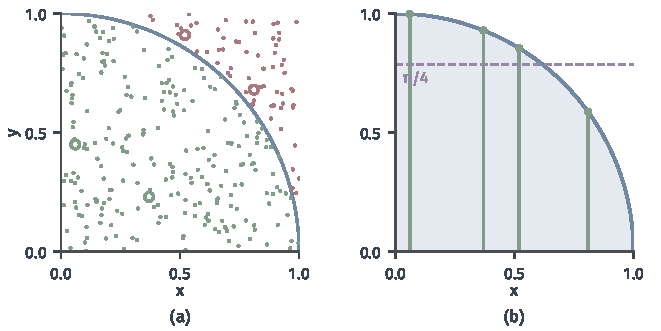
\includegraphics[width=112mm]{figures/07-probability/08-sampling-and-integration/matplotlib/vr-conditional/figure.pdf}
 \caption{用条件期望计算$\mathbb{P}(X^2+Y^2\leq1)=\pi/4$。(a)单位正方形中的$300$个随机点（种子2），圆内为绿色、圆外为红色，四个空心圆为正文的手算点；蓝线是四分之一圆周。(b)蓝线为$g(x)=\sqrt{1-x^2}$，绿色竖线是四个手算点的$x$处整条竖直切片在圆内的比例，紫色虚线为$\pi/4$。}
 \label{fig:vr-conditional}
\end{BookInlineFigure}

图~\ref{fig:vr-conditional}对比了两种计算。左图每个点只给出$0$或$1$；右图每个$x$给出整条竖直切片落在圆内的比例，样本之间的差别只来自$x$的不同。这里$g$只需一次开方，每个样本还少抽一个均匀数，成本不增反减。一般情形下，计算$g$可能需要一个积分，它的成本必须计入。

\paragraph{条件平均只能近似时}
若$g$没有闭式，需要用数值方法近似，定理~\ref{thm:vr-conditioning}的保证不能直接沿用，要看近似怎样做。

一种做法是确定性的求积。例如在每个$x$处，用$m$个等距中点$y_j=(j-\tfrac12)/m$数出满足$x^2+y_j^2\leq1$的比例，作为$g(x)$的近似$g_m(x)$。这个量不是$f$的条件期望，$\mathbb{E}[g_m(X)]\neq I$，产生一个不随$n$减小的偏差，需要像数值积分那样单独估计它的大小。

另一种做法是在每个$X_i$处再独立抽$m$个$Y_{i,1},\dots,Y_{i,m}$，平均$f(X_i,Y_{i,j})$。给定$X_i$时这$m$项独立同分布，所以内层平均的条件期望仍是$g(X_i)$，估计无偏。由全方差公式，内层平均的方差为
\[
 \operatorname{Var}\bigl(g(X)\bigr)+\frac{\mathbb{E}\bigl[\operatorname{Var}(f\mid X)\bigr]}{m} .
\]
$m=1$时回到直接平均，$m\to\infty$时趋于条件Monte Carlo，代价是每个外层样本做$m$次内层计算。四分之一圆中取$m=2$，方差为$0.0498+0.1187/2\approx0.1092$。


\section{改变抽样机制}
\label{sec:vr-change-mechanism}

前两节的方法都保持样本之间相互独立。独立有它的代价：$n$个独立均匀点可能挤在一处，也可能留下大片空白，每个区域分到多少样本完全由运气决定。本节放弃样本之间的独立，转而有计划地安排基础随机数：规定每个区域分到的点数，让点集整体上铺得均匀，或者让成对的输出朝相反或相同的方向变化。每个点的边缘分布仍然正确，所以估计仍然无偏；变化的是点与点之间的协方差。

\paragraph{把积分搬到单位立方体上}
设第~\ref{chap:sample-generation}章给出了一个可计算的生成映射$T:[0,1)^d\to\mathcal{X}$，使$\bm{U}\sim\operatorname{Unif}([0,1)^d)$时$T(\bm{U})\sim P$。记$F=f\circ T$，则
\begin{equation}
 I=\mathbb{E}_P[f(X)]=\int_{[0,1)^d}F(\bm{u})\,\mathrm{d}\bm{u} .
 \label{eq:vr-unit-cube}
\end{equation}
例如相关的高斯向量$\mathcal{N}(\bm{\mu},\bm{\Sigma})$可以取
\[
 T(\bm{u})=\bm{\mu}+\bm{L}\bigl(\Phi^{-1}(u_1),\dots,\Phi^{-1}(u_d)\bigr)^{\top} ,
\]
其中$\bm{L}$是协方差矩阵$\bm{\Sigma}$的Cholesky因子。点集的安排都在$\bm{u}$上进行，目标坐标之间的相关结构由$T$负责保留。这样，本节的方法只需要处理“单位立方体上的均匀点”这一种对象；代价是它们的效果取决于$F=f\circ T$的性质，而不仅是$f$的性质。

\subsection{分层采样}
\label{sec:vr-stratified}

用$8$个独立均匀点计算$\int_0^1\mathrm{e}^{u}\,\mathrm{d}u$，落在左半区间的点数服从$\operatorname{Bin}(8,1/2)$，有$7\%$的机会是$0$、$1$、$7$或$8$个。左半区间的函数值小、右半区间的大，点数的偶然多少直接变成估计的偏高或偏低。如果事先规定每个子区间各放几个点，这部分波动就消失了。

\begin{definition}[分层采样估计]
\label{def:vr-stratified}
把$\mathcal{X}$分成互不相交的集合$A_1,\dots,A_K$，称为层，设各层概率$p_k=P(A_k)>0$已知，并且能从条件分布$P(\cdot\mid A_k)$抽样。取正整数$n_1,\dots,n_K$，$\sum_kn_k=n$。各层内独立抽取$X_{k,1},\dots,X_{k,n_k}\sim P(\cdot\mid A_k)$，层间也相互独立。称
\begin{equation}
 \hat{I}^{\mathrm{st}}=\sum_{k=1}^{K}p_k\,\hat{\mu}_k,\qquad \hat{\mu}_k=\frac{1}{n_k}\sum_{i=1}^{n_k}f(X_{k,i})
 \label{eq:vr-stratified}
\end{equation}
为\term{分层采样}（stratified sampling）估计。
\end{definition}

记层内均值与层内方差为
\[
 \mu_k=\mathbb{E}[f(X)\mid X\in A_k],\qquad \sigma_k^2=\operatorname{Var}\bigl(f(X)\bigm|X\in A_k\bigr) .
\]

\begin{theorem}[分层估计的方差]
\label{thm:vr-stratified}
设$\mathbb{E}_P[f^2]<\infty$。则$\hat{I}^{\mathrm{st}}$无偏，且
\begin{equation}
 \operatorname{Var}\bigl(\hat{I}^{\mathrm{st}}\bigr)=\sum_{k=1}^{K}\frac{p_k^2\,\sigma_k^2}{n_k} .
 \label{eq:vr-stratified-variance}
\end{equation}
若按\term{比例分配}（proportional allocation）取$n_k=np_k$，则
\begin{equation}
 \operatorname{Var}\bigl(\hat{I}^{\mathrm{st}}\bigr)=\frac1n\sum_{k=1}^{K}p_k\sigma_k^2=\frac{\sigma^2}{n}-\frac1n\sum_{k=1}^{K}p_k(\mu_k-I)^2\leq\frac{\sigma^2}{n} .
 \label{eq:vr-proportional}
\end{equation}
\end{theorem}

\begin{proof}
由全概率公式，$\sum_kp_k\mu_k=I$；每个$\hat{\mu}_k$是$\mu_k$的无偏估计，所以$\hat{I}^{\mathrm{st}}$无偏。各层的样本相互独立，方差相加；$\hat{\mu}_k$的方差为$\sigma_k^2/n_k$，乘以系数的平方$p_k^2$即为第$k$层的贡献。

比例分配时代入$n_k=np_k$即得第一个等号。把层号$J$（$X\in A_J$）看成一个离散随机变量，由全方差公式，
\[
 \sigma^2=\mathbb{E}\bigl[\operatorname{Var}(f\mid J)\bigr]+\operatorname{Var}\bigl(\mathbb{E}[f\mid J]\bigr)=\sum_kp_k\sigma_k^2+\sum_kp_k(\mu_k-I)^2 ,
\]
移项得第二个等号。
\end{proof}

式~\eqref{eq:vr-proportional}说明比例分配的分层永远不比独立抽样差：它把总方差中的层间部分$\sum_kp_k(\mu_k-I)^2$整个去掉了。这一部分正是“各层分到多少点由运气决定”造成的波动。层分得越细、层均值差别越大，去掉的越多。

\paragraph{考虑波动与成本的分配}
比例分配没有利用各层的波动大小。设第$k$层每个样本的成本为$c_k$，总预算为$\sum_kc_kn_k=C$，在式~\eqref{eq:vr-stratified-variance}中选$n_k$。暂时允许$n_k$取正实数，由Cauchy--Schwarz不等式，
\[
 \Bigl(\sum_kp_k\sigma_k\sqrt{c_k}\Bigr)^2=\Bigl(\sum_k\frac{p_k\sigma_k}{\sqrt{n_k}}\cdot\sqrt{c_kn_k}\Bigr)^2\leq\Bigl(\sum_k\frac{p_k^2\sigma_k^2}{n_k}\Bigr)\Bigl(\sum_kc_kn_k\Bigr) .
\]
右边第二个因子是$C$，所以方差不小于$(\sum_kp_k\sigma_k\sqrt{c_k})^2/C$。等号当且仅当两个因子成比例，即
\begin{equation}
 n_k\propto\frac{p_k\sigma_k}{\sqrt{c_k}},\qquad \operatorname{Var}\bigl(\hat{I}^{\mathrm{st}}\bigr)_{\min}=\frac{\bigl(\sum_kp_k\sigma_k\sqrt{c_k}\bigr)^2}{C} .
 \label{eq:vr-neyman}
\end{equation}
波动大的层多放点，昂贵的层少放点。各层成本相同时$n_k\propto p_k\sigma_k$，称为\term{Neyman分配}（Neyman allocation）。实际的$n_k$要取整；若还要在层内估计方差，每层至少需要两个点。

\paragraph{例子：四层计算$\mathrm{e}-1$}
把$[0,1)$等分为四层，$p_k=1/4$。在宽为$1/4$的区间$[a,a+\tfrac14)$上，层均值与层内方差可以直接积分：
\[
 \mu_k=4\bigl(\mathrm{e}^{a+1/4}-\mathrm{e}^{a}\bigr),\qquad \sigma_k^2=2\bigl(\mathrm{e}^{2a+1/2}-\mathrm{e}^{2a}\bigr)-\mu_k^2 .
\]
四层的结果为
\[
 \begin{array}{lcccc}
  \text{层} & [0,\tfrac14) & [\tfrac14,\tfrac12) & [\tfrac12,\tfrac34) & [\tfrac34,1)\\
  \mu_k & 1.1361 & 1.4588 & 1.8731 & 2.4051\\
  \sigma_k & 0.0819 & 0.1052 & 0.1351 & 0.1735
 \end{array}
\]
取$n=8$，比例分配每层$2$个点，由式~\eqref{eq:vr-proportional}，
\[
 \operatorname{Var}\bigl(\hat{I}^{\mathrm{st}}\bigr)=\frac18\cdot\frac14\sum_k\sigma_k^2\approx0.002067 ,
\]
而$8$个独立点的方差为$0.24204/8\approx0.03025$，降为$1/14.6$。Neyman分配按$\sigma_k$的比例给出$n_k\approx1.32,1.70,2.18,2.80$，方差降到$0.001920$；取整为$1,2,2,3$时为$0.001963$，但第一层只有一个点，无法估计它的层内方差。这里各层波动相差不到三倍，最优分配只比比例分配好$7\%$。

下面用八个层内均匀数演示比例分配的计算，第$k$层的点取$u=(k-1+v)/4$：
\[
 v=0.37,\ 0.81\ \big|\ 0.06,\ 0.52\ \big|\ 0.23,\ 0.68\ \big|\ 0.45,\ 0.91 .
\]
得到的八个点依次为
\[
 u=0.0925,\ 0.2025,\ 0.265,\ 0.38,\ 0.5575,\ 0.67,\ 0.8625,\ 0.9775 .
\]
层均值的估计是每层两个$\mathrm{e}^{u}$的平均，再按$p_k=1/4$加权；因为比例分配，这等于八个函数值的普通平均：
\[
 \hat{I}^{\mathrm{st}}=\frac18\bigl(1.0969+1.2245+\cdots+2.6578\bigr)=1.7268 .
\]
真值为$1.7183$。

\begin{BookInlineFigure}
 \centering
 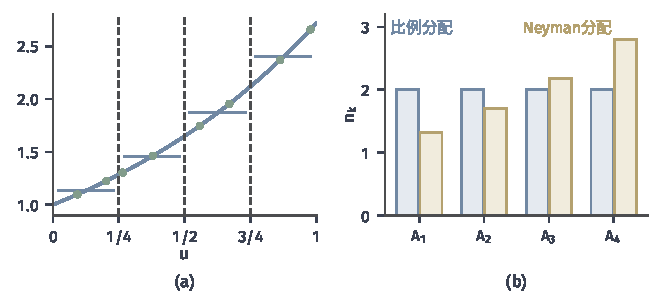
\includegraphics[width=112mm]{figures/07-probability/08-sampling-and-integration/matplotlib/vr-stratified/figure.pdf}
 \caption{四层分层采样计算$\int_0^1\mathrm{e}^{u}\,\mathrm{d}u$。(a)蓝线为$\mathrm{e}^{u}$，虚线为层的边界，蓝色短横线为层均值$\mu_k$，绿点为每层两个样本（$v$见正文）。(b)$n=8$时的样本分配：蓝色为比例分配$n_k=2$，黄色为Neyman分配$n_k\propto\sigma_k$。}
 \label{fig:vr-stratified}
\end{BookInlineFigure}

\paragraph{层越细越好，但维数会让层数爆炸}
图~\ref{fig:vr-stratified}(a)中，层内的函数几乎是直线，层内波动远小于整体波动。把$[0,1)$等分成$n$层、每层一个点，式~\eqref{eq:vr-stratified-variance}成为$n^{-2}\sum_k\sigma_k^2$。若$\lvert F'\rvert\leq L$，宽为$1/n$的层上$F$的取值范围不超过$L/n$，层内方差不超过$(L/n)^2/4$，于是
\[
 \operatorname{Var}\bigl(\hat{I}^{\mathrm{st}}\bigr)\leq\frac{1}{n^2}\cdot n\cdot\frac{L^2}{4n^2}=\frac{L^2}{4n^3} .
\]
方差按$n^{-3}$而非$n^{-1}$下降。到了$d$维，把每个坐标分成$m$段需要$m^d$个层，$d=10$、$m=2$就已经是$1024$层，每层至少一个点；预算不足$m^d$时，联合分层根本无法实施。

\paragraph{层的概率与分配不能由同一批数据随意决定}
定理~\ref{thm:vr-stratified}假设$p_k$已知、$n_k$事先固定。若$p_k$本身要从样本估计，估计量就变成两个随机量的组合，偏差和方差都要重新推导。若$n_k$按一次独立的试运行估计的$\sigma_k$确定，那么给定试运行结果，分配是固定的，定理的结论在条件意义下仍然成立；若边抽样边根据已抽到的值调整$n_k$，各层的样本数依赖于样本本身，式~\eqref{eq:vr-stratified-variance}不能直接套用，需要另行分析。

\subsection{拉丁超立方采样}
\label{sec:vr-lhs}

联合分层在高维失效，但退一步，可以只要求每个坐标各自分层：$n$个点投影到任何一根坐标轴上，都恰好在$n$个等长小区间中各占一个。这样，无论维数多大，$n$个点就够了。

\begin{definition}[拉丁超立方设计]
\label{def:vr-lhs}
给定点数$n$与维数$d$。取$d$个相互独立、在$\{1,\dots,n\}$的全部排列上均匀分布的随机排列$\pi_1,\dots,\pi_d$，再取与它们独立的$V_{i,j}\sim\operatorname{Unif}(0,1)$，$i=1,\dots,n$，$j=1,\dots,d$，全部相互独立。令
\begin{equation}
 U_{i,j}=\frac{\pi_j(i)-1+V_{i,j}}{n},\qquad \bm{U}_i=(U_{i,1},\dots,U_{i,d}) ,
 \label{eq:vr-lhs}
\end{equation}
用
\begin{equation}
 \hat{I}^{\mathrm{LHS}}=\frac1n\sum_{i=1}^{n}F(\bm{U}_i)
 \label{eq:vr-lhs-estimator}
\end{equation}
估计式~\eqref{eq:vr-unit-cube}的积分。
\end{definition}

第$i$个点的第$j$个坐标落在第$\pi_j(i)$层，层内位置由$V_{i,j}$决定。因为$\pi_j$是排列，第$j$个坐标的$n$个值恰好每层一个。这种设计称为拉丁超立方采样（Latin hypercube sampling，LHS），也叫\term{拉丁超立方抽样}。

\begin{theorem}[拉丁超立方的无偏性]
\label{thm:vr-lhs-unbiased}
在定义~\ref{def:vr-lhs}中，每个$\bm{U}_i$都服从$\operatorname{Unif}([0,1)^d)$。所以对可积的$F$，$\mathbb{E}[\hat{I}^{\mathrm{LHS}}]=I$。
\end{theorem}

\begin{proof}
固定$i$与$j$。均匀随机排列下$\pi_j(i)$在$\{1,\dots,n\}$上均匀分布，且与$V_{i,j}$独立。对$t\in[0,1]$，按层号分解，
\[
 \begin{aligned}
 \mathbb{P}(U_{i,j}\leq t)&=\sum_{k=1}^{n}\frac1n\,\mathbb{P}\Bigl(\frac{k-1+V_{i,j}}{n}\leq t\Bigr)\\
 &=\sum_{k=1}^{n}\frac1n\min\bigl\{1,\max\{0,nt-k+1\}\bigr\}=t .
 \end{aligned}
\]
最后一步中，$t$所在层之前的各层贡献$1/n$，$t$所在层贡献其中的一部分，之后的各层贡献$0$。不同的$j$用的是相互独立的$(\pi_j,V_{1,j},\dots,V_{n,j})$，所以$U_{i,1},\dots,U_{i,d}$相互独立，$\bm{U}_i$在立方体上均匀。对$n$个点的$F$值取期望并平均，得到无偏性。
\end{proof}

\paragraph{二维四点}
取$n=4$，$d=2$，两个排列与层内位置为
\[
 \pi_1=(2,4,1,3),\qquad \pi_2=(1,3,2,4) ,
\]
\[
 V_{:,1}=(0.37,0.81,0.06,0.52),\qquad V_{:,2}=(0.23,0.68,0.45,0.91) .
\]
由式~\eqref{eq:vr-lhs}，第一个点为
\[
 \bm{U}_1=\Bigl(\frac{1+0.37}{4},\ \frac{0+0.23}{4}\Bigr)=(0.3425,0.0575) .
\]
同样得到
\[
 \bm{U}_2=(0.9525,0.67),\qquad \bm{U}_3=(0.015,0.3625),\qquad \bm{U}_4=(0.63,0.9775) .
\]
图~\ref{fig:vr-lhs-points}(a)把单位正方形分成$4\times4$个格子：每行、每列恰好一个点，但$16$个格子只占了$4$个。逐维覆盖不等于覆盖全部坐标组合。图(b)是另一种同样合法的设计，两个排列都取恒等排列，四个点全落在对角线的格子里，坐标之间几乎完全相关。这种设计出现的概率是$1/4!$，它提醒我们：拉丁超立方只控制每个坐标的投影，不控制点在平面上的整体分布。

\begin{BookInlineFigure}
 \centering
 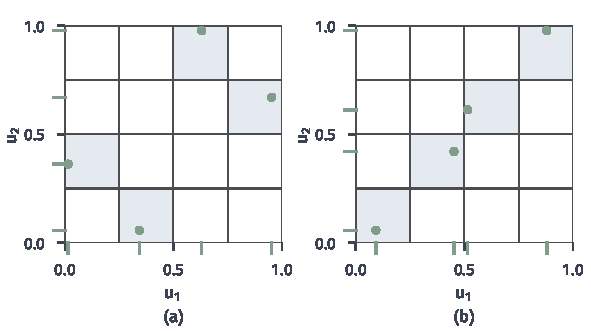
\includegraphics[width=100mm]{figures/07-probability/08-sampling-and-integration/matplotlib/vr-lhs-points/figure.pdf}
 \caption{$n=4$、$d=2$的拉丁超立方设计。灰线把正方形分成$4\times4$格，浅蓝格子含有一个点，坐标轴旁的绿色短线是点在各坐标上的投影。(a)$\pi_1=(2,4,1,3)$，$\pi_2=(1,3,2,4)$；(b)两个排列都是恒等排列。两者的$V$相同，见正文。}
 \label{fig:vr-lhs-points}
\end{BookInlineFigure}

对$F(\bm{u})=\mathrm{e}^{u_1}+\mathrm{e}^{u_2}$，真值$2(\mathrm{e}-1)=3.4366$。图(a)的四个点给出两列函数值的平均$1.7233$与$1.7770$，估计为$3.5004$。

\paragraph{可加函数：每个坐标都得到分层的好处}
先看$F$可以写成各坐标函数之和的情形。

\begin{theorem}[可加函数的拉丁超立方方差]
\label{thm:vr-lhs-additive}
设$F(\bm{u})=c+\sum_{j=1}^{d}g_j(u_j)$，各$g_j(U)$平方可积。记$\sigma_{j,k}^2$为$g_j(V)$在$V\sim\operatorname{Unif}([\tfrac{k-1}{n},\tfrac{k}{n}))$下的方差。则
\begin{equation}
 \operatorname{Var}\bigl(\hat{I}^{\mathrm{LHS}}\bigr)=\frac{1}{n^2}\sum_{j=1}^{d}\sum_{k=1}^{n}\sigma_{j,k}^2\leq\frac1n\sum_{j=1}^{d}\operatorname{Var}\bigl(g_j(U)\bigr) .
 \label{eq:vr-lhs-additive}
\end{equation}
\end{theorem}

\begin{proof}
估计量拆成$c+\sum_jT_j$，其中$T_j=\frac1n\sum_ig_j(U_{i,j})$只依赖第$j$列。第$j$列的$n$个值恰好每层一个，层内位置独立均匀，所以$T_j$正是每层一个点、$p_k=1/n$的分层估计，由式~\eqref{eq:vr-stratified-variance}，它的方差为$n^{-2}\sum_k\sigma_{j,k}^2$。不同列由相互独立的排列与层内位置生成，$T_1,\dots,T_d$相互独立，方差相加，得到等式。不等式是式~\eqref{eq:vr-proportional}对每一列的应用。
\end{proof}

对$F=\mathrm{e}^{u_1}+\mathrm{e}^{u_2}$，独立抽样的单点方差是$2\times0.24204$，而由上一小节的论证，式~\eqref{eq:vr-lhs-additive}按$n^{-3}$下降。图~\ref{fig:vr-lhs-variance}中绿线是比值$n\operatorname{Var}(\hat{I}^{\mathrm{LHS}})/\sigma^2$，它以$n^{-2}$的速度趋于零。

\paragraph{交互项：可能比独立抽样更差}
再看一个没有任何可加部分的函数。令$s(t)=1$（$t\geq\tfrac12$）或$-1$（$t<\tfrac12$），
\[
 F(\bm{u})=s(u_1)\,s(u_2) .
\]
$I=0$，$\sigma^2=1$，独立抽样的方差为$1/n$。设$n$为偶数，则第一个坐标落在下半区间$[0,\tfrac12)$的点恰有$n/2$个，第二个坐标也是。记$N$为两个坐标都在下半区间的点数。由$\pi_2$与$\pi_1$独立，第二个坐标落在下半区间的那些点是从$n$个点中均匀抽取的$n/2$个，所以$N$服从超几何分布$\operatorname{Hyp}(n,n/2,n/2)$。四类点的个数分别为
\[
 \text{下下}=N,\qquad \text{下上}=\text{上下}=\frac n2-N,\qquad \text{上上}=N .
\]

$F$在下下与上上处为$1$，其余为$-1$，于是
\[
 \hat{I}^{\mathrm{LHS}}=\frac{2N-2(n/2-N)}{n}=\frac{4N-n}{n} .
\]
由第~\ref{chap:common-distributions}章超几何分布的方差，
\[
 \operatorname{Var}(N)=\frac n2\cdot\frac12\cdot\frac12\cdot\frac{n-n/2}{n-1}=\frac{n^2}{16(n-1)} .
\]
所以
\begin{equation}
 \operatorname{Var}\bigl(\hat{I}^{\mathrm{LHS}}\bigr)=\frac{16}{n^2}\operatorname{Var}(N)=\frac{1}{n-1}>\frac1n .
 \label{eq:vr-lhs-interaction}
\end{equation}
$n=2$时方差为$1$，是独立抽样$1/2$的两倍：两点必然一个在左下或右上、另一个在相反的角，两个函数值相同，等于只抽了一个点。

\begin{BookInlineFigure}
 \centering
 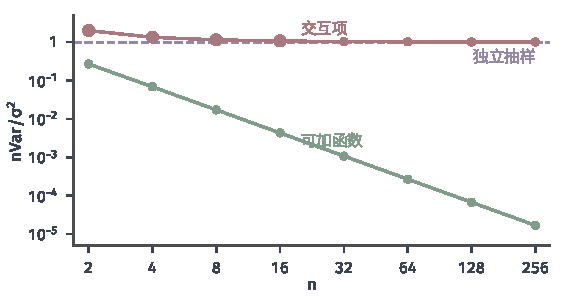
\includegraphics[width=96mm]{figures/07-probability/08-sampling-and-integration/matplotlib/vr-lhs-variance/figure.pdf}
 \caption{拉丁超立方的方差与独立抽样之比$n\operatorname{Var}(\hat{I}^{\mathrm{LHS}})/\sigma^2$，双对数坐标，$n$为偶数。绿线为可加函数$\mathrm{e}^{u_1}+\mathrm{e}^{u_2}$，按式~\eqref{eq:vr-lhs-additive}精确计算；红线为交互函数$s(u_1)s(u_2)$的精确值$n/(n-1)$，空心圆是$2\times10^{4}$次模拟（种子8）；紫色虚线为独立抽样。}
 \label{fig:vr-lhs-variance}
\end{BookInlineFigure}

\paragraph{一般函数}
一般的平方可积$F$可以分解为常数、各坐标的主效应$g_j(u_j)=\mathbb{E}[F(\bm{U})\mid U_j=u_j]-I$和剩下的交互部分。已知的结论是：拉丁超立方的方差等于$\sigma^2/n$减去$\frac1n\sum_j\operatorname{Var}(g_j(U_j))$，再加一个比$1/n$高阶的项；并且对任何平方可积的$F$和$n\geq2$，方差不超过$\sigma^2/(n-1)$。前者说明它去掉的正是主效应，后者说明它最多比独立抽样差一个因子$n/(n-1)$，式~\eqref{eq:vr-lhs-interaction}恰好达到这个上界。这两个结论的证明需要对排列做较长的组合计算，这里只用它们解释图~\ref{fig:vr-lhs-variance}：$F$越接近可加，拉丁超立方越有效；$F$以交互为主时，它几乎没有好处，有限样本下还可能略差。

\paragraph{误差怎样估计}
同一设计中的$n$个点不独立，它们的$F$值的样本方差除以$n$不是$\operatorname{Var}(\hat{I}^{\mathrm{LHS}})$的估计。正确的做法是第~\ref{chap:monte-carlo-integration-error}章的整组重复：独立生成$R$个设计，得到$R$个估计$Q_1,\dots,Q_R$，总平均$\bar{Q}$的方差用$s_Q^2/R$估计，$s_Q^2$是$Q_r$的样本方差。

\subsection{随机化准蒙特卡洛}
\label{sec:vr-rqmc}

分层与拉丁超立方都只控制点在若干固定格子中的个数。更直接的想法是：让点集在任何位置、任何尺度上都铺得均匀。先要有一个衡量“铺得均不均匀”的量。

对$\bm{b}\in[0,1]^d$，考虑以原点为一角的盒子$[\bm{0},\bm{b})=[0,b_1)\times\cdots\times[0,b_d)$。点集$\bm{a}_1,\dots,\bm{a}_n$均匀时，落进盒子的点的比例应当接近盒子的体积。

\begin{definition}[星差异]
\label{def:vr-star-discrepancy}
点集$\bm{a}_1,\dots,\bm{a}_n\in[0,1)^d$的\term{星差异}（star discrepancy）为
\begin{equation}
 D_n^{*}=\sup_{\bm{b}\in[0,1]^d}\Bigl\lvert\frac{\#\{i:\bm{a}_i\in[\bm{0},\bm{b})\}}{n}-\prod_{j=1}^{d}b_j\Bigr\rvert .
 \label{eq:vr-star-discrepancy}
\end{equation}
\end{definition}

一维时容易算。等距点$a_i=(i-1)/n$在$b$略大于$(i-1)/n$时，盒子里有$i$个点而长度只有约$(i-1)/n$，差$1/n$，所以$D_n^{*}=1/n$。把它们右移半格成$a_i=(i-\tfrac12)/n$，最大偏差减半为$1/(2n)$。$n=4$时，前者为$1/4$，后者为$1/8$。

图~\ref{fig:vr-discrepancy}比较了二维的两组$13$个点。独立均匀点（种子4）中，盒子$[0,0.607)\times[0,1)$的体积为$0.607$，却只含$3$个点，比例$0.231$，差$0.377$，这就是它的星差异。右图是一种规则构造：
\[
 \bm{a}_i=\Bigl(\frac{i-1}{13},\ \Bigl\{\frac{8(i-1)}{13}\Bigr\}\Bigr),\qquad i=1,\dots,13 ,
\]
其中$\{x\}=x-\lfloor x\rfloor$表示小数部分。它的星差异为$0.166$，由盒子$[0,0.538]\times[0,0.692]$达到：盒子连同边界上的点共$7$个，比例$0.538$，体积$0.373$。

\begin{BookInlineFigure}
 \centering
 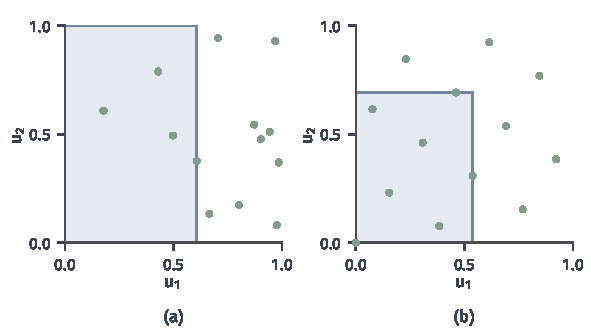
\includegraphics[width=100mm]{figures/07-probability/08-sampling-and-integration/matplotlib/vr-discrepancy/figure.pdf}
 \caption{$13$个点的星差异。浅蓝矩形是取到式~\eqref{eq:vr-star-discrepancy}中上确界的锚定盒子。(a)独立均匀点（种子4），盒子$[0,0.607)\times[0,1)$内只有$3$个点，$D_{13}^{*}=0.377$；(b)格点$((i-1)/13,\{8(i-1)/13\})$，盒子$[0,0.538]\times[0,0.692]$连同边界含$7$个点，$D_{13}^{*}=0.166$。}
 \label{fig:vr-discrepancy}
\end{BookInlineFigure}

\paragraph{确定性点集的积分误差}
用一个确定的点集代替随机样本，直接平均各点上的函数值，称为\term{准蒙特卡洛}（quasi-Monte Carlo）方法。它的误差由一个把函数与点集分开的不等式控制，称为\term{Koksma--Hlawka不等式}（Koksma--Hlawka inequality）：
\begin{equation}
 \Bigl\lvert\frac1n\sum_{i=1}^{n}F(\bm{a}_i)-\int_{[0,1)^d}F(\bm{u})\,\mathrm{d}\bm{u}\Bigr\rvert\leq V_{\mathrm{HK}}(F)\,D_n^{*} ,
 \label{eq:vr-koksma-hlawka}
\end{equation}
其中$V_{\mathrm{HK}}(F)$是$F$在Hardy--Krause意义下的变差，一维时就是$F$的全变差。证明需要多元的分部求和与变差的定义，篇幅较长。它的含义是：误差等于函数的起伏程度乘以点集的不均匀程度。一维的情形可以直接体会：$F$单调时，误差不超过$F$的总升降乘以$D_n^{*}$。

已有构造能使$D_n^{*}$随$n$按$(\ln n)^d/n$的阶下降，这样的点集称为\term{低差异点集}（low-discrepancy point set）；独立均匀点的星差异只按$n^{-1/2}$的阶下降。于是对$V_{\mathrm{HK}}(F)<\infty$的函数，准蒙特卡洛的误差在$n$很大时比$n^{-1/2}$小得多。但式~\eqref{eq:vr-koksma-hlawka}有三个局限：$V_{\mathrm{HK}}(F)$对无界函数和边界倾斜的示性函数是无穷；两个因子都难以计算，界本身不能用来报告误差；点集是确定的，算一次得到一个数，没有任何关于误差大小的信息。

\paragraph{加入随机性}
解决最后一个问题的办法是把整组点随机化：施加一个随机变换，使每个点单独看都服从均匀分布，而点集的均匀结构保持不变。这样得到的方法称为\term{随机化准蒙特卡洛}（randomized quasi-Monte Carlo，RQMC）。每个点均匀，保证估计无偏；整组独立重复若干次，就可以用第~\ref{chap:monte-carlo-integration-error}章的组间方差估计误差。下面讨论最简单的随机化，以及误差衰减的速度由什么决定。

\subsubsection{随机移位}
\label{sec:vr-random-shift}

把单位立方体的相对两面粘起来，它就成为一个环面：从右边出去的点从左边回来。在环面上整体平移一个点集，点与点之间的相对位置不变。

\begin{definition}[随机移位]
\label{def:vr-random-shift}
给定点集$\bm{a}_1,\dots,\bm{a}_n\in[0,1)^d$，取$\bm{\Delta}\sim\operatorname{Unif}([0,1)^d)$，令
\begin{equation}
 \bm{U}_i=(\bm{a}_i+\bm{\Delta})\bmod1,\qquad i=1,\dots,n ,
 \label{eq:vr-random-shift}
\end{equation}
其中$\bmod1$逐坐标取小数部分。所有点共用同一个$\bm{\Delta}$。称$Q=\frac1n\sum_iF(\bm{U}_i)$为\term{随机移位}（random shift）估计。
\end{definition}

例如$a=0.75$、$\Delta=0.37$时，$a+\Delta=1.12$，取小数部分得$0.12$：点从右端越过$1$后回到左端。图~\ref{fig:vr-random-shift}把上面的$13$点格点整体平移$\bm{\Delta}=(0.37,0.81)$：左图中平移后的点散在$[0,2)^2$的四块单位正方形里，右图把它们按$\bmod1$折回$[0,1)^2$，得到的仍是同一个格点结构，只是整体挪了位置。

\begin{BookInlineFigure}
 \centering
 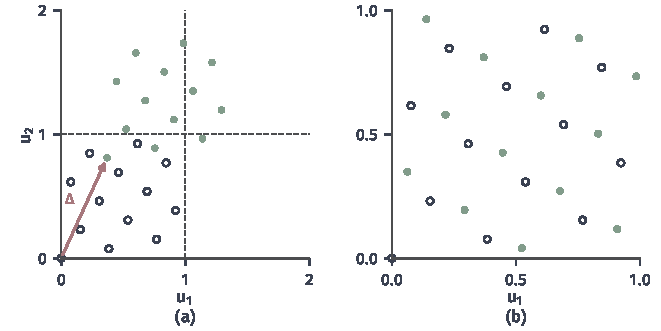
\includegraphics[width=112mm]{figures/07-probability/08-sampling-and-integration/matplotlib/vr-random-shift/figure.pdf}
 \caption{对$13$点格点的随机移位，$\bm{\Delta}=(0.37,0.81)$。空心圆为原格点，红色箭头为$\bm{\Delta}$。(a)平移后的点$\bm{a}_i+\bm{\Delta}$（绿色），虚线把$[0,2)^2$分成四块单位正方形；(b)逐坐标取小数部分后的$\bm{U}_i$（绿色）。}
 \label{fig:vr-random-shift}
\end{BookInlineFigure}

\begin{theorem}[随机移位的无偏性与方差]
\label{thm:vr-random-shift}
在定义~\ref{def:vr-random-shift}中，每个$\bm{U}_i$都服从$\operatorname{Unif}([0,1)^d)$，所以对可积的$F$，$\mathbb{E}[Q]=I$。若$F$平方可积，记其Fourier系数与点集的指数和为
\begin{equation}
 \begin{gathered}
 \hat{F}(\bm{h})=\int_{[0,1)^d}F(\bm{u})\mathrm{e}^{-2\pi\mathrm{i}\langle\bm{h},\bm{u}\rangle}\,\mathrm{d}\bm{u},\\
 S(\bm{h})=\frac1n\sum_{i=1}^{n}\mathrm{e}^{2\pi\mathrm{i}\langle\bm{h},\bm{a}_i\rangle},\qquad \bm{h}\in\mathbb{Z}^d ,
 \end{gathered}
 \label{eq:vr-fourier-sum}
\end{equation}
则
\begin{equation}
 \operatorname{Var}(Q)=\sum_{\bm{h}\neq\bm{0}}\bigl\lvert\hat{F}(\bm{h})\bigr\rvert^2\bigl\lvert S(\bm{h})\bigr\rvert^2 .
 \label{eq:vr-shift-variance}
\end{equation}
\end{theorem}

\begin{proof}
先证均匀性。一维时，固定$a\in[0,1)$，映射$\delta\mapsto(a+\delta)\bmod1$把$[0,1-a)$平移$a$得到$[a,1)$，把$[1-a,1)$平移$a-1$得到$[0,a)$，两段平移都保持长度，所以它把$[0,1)$上的均匀分布映成均匀分布。$d$维时$\bm{\Delta}$的各坐标独立，$\bm{U}_i$的各坐标也就独立且各自均匀。对$n$个点平均并取期望，得到无偏性。

再算方差。把$Q$看成$\bm{\Delta}$的函数：
\[
 Q(\bm{\Delta})=\frac1n\sum_{i=1}^{n}F\bigl((\bm{a}_i+\bm{\Delta})\bmod1\bigr) .
\]由平移保持均匀分布，每一项与$F$有相同的$L^2$范数，所以$Q$平方可积。

计算$Q$的Fourier系数时，对第$i$项作变量替换$\bm{v}=(\bm{a}_i+\bm{\Delta})\bmod1$，这一替换保持均匀测度。因为$\bm{h}$是整数向量，取小数部分不改变指数：
\[
 \mathrm{e}^{-2\pi\mathrm{i}\langle\bm{h},\bm{\Delta}\rangle}=\mathrm{e}^{-2\pi\mathrm{i}\langle\bm{h},\bm{v}\rangle}\,\mathrm{e}^{2\pi\mathrm{i}\langle\bm{h},\bm{a}_i\rangle} .
\]
于是
\[
 \hat{Q}(\bm{h})=\frac1n\sum_{i=1}^{n}\mathrm{e}^{2\pi\mathrm{i}\langle\bm{h},\bm{a}_i\rangle}\int_{[0,1)^d}F(\bm{v})\mathrm{e}^{-2\pi\mathrm{i}\langle\bm{h},\bm{v}\rangle}\,\mathrm{d}\bm{v}=\hat{F}(\bm{h})\,S(\bm{h}) .
\]

函数族$\mathrm{e}^{2\pi\mathrm{i}\langle\bm{h},\bm{u}\rangle}$（$\bm{h}\in\mathbb{Z}^d$）是$L^2([0,1)^d)$的完备正交规范系（可参考\BookChapterRef{chap:fourier-transform}{卷四第14章“Fourier变换”}），由Parseval等式（可参考\BookChapterRef{chap:function-inner-product-spaces}{卷四第12章“内积空间”}），
\[
 \mathbb{E}\bigl[\lvert Q\rvert^2\bigr]=\sum_{\bm{h}\in\mathbb{Z}^d}\bigl\lvert\hat{F}(\bm{h})S(\bm{h})\bigr\rvert^2 .
\]
$\bm{h}=\bm{0}$一项是$\lvert\hat{F}(\bm{0})\rvert^2=I^2$，因为$S(\bm{0})=1$。减去$I^2$即得式~\eqref{eq:vr-shift-variance}。
\end{proof}

\paragraph{点集是一个频率滤波器}
把式~\eqref{eq:vr-shift-variance}与独立抽样比较。对$F$本身用Parseval等式，
\[
 \sigma^2=\sum_{\bm{h}\neq\bm{0}}\bigl\lvert\hat{F}(\bm{h})\bigr\rvert^2 ,
\]
所以独立抽样的方差$\sigma^2/n$相当于给每个频率都乘上$1/n$。随机移位则给频率$\bm{h}$乘上$\lvert S(\bm{h})\rvert^2$。好的点集让$S(\bm{h})$在低频处为零或很小，只在少数高频处较大；只要$F$的能量主要集中在低频，方差就远小于$\sigma^2/n$。

格点是最干净的例子。取整数向量$\bm{z}$，令$\bm{a}_i=\{(i-1)\bm{z}/n\}$（逐坐标取小数部分）。$S(\bm{h})$是$n$个单位根的平均：若$\langle\bm{h},\bm{z}\rangle$是$n$的倍数，每项都是$1$，$S(\bm{h})=1$；否则$\mathrm{e}^{2\pi\mathrm{i}\langle\bm{h},\bm{z}\rangle/n}\neq1$，等比数列求和得$S(\bm{h})=0$。于是
\begin{equation}
 \operatorname{Var}(Q)=\sum_{\bm{h}\neq\bm{0},\ \langle\bm{h},\bm{z}\rangle\equiv0\ (\mathrm{mod}\ n)}\bigl\lvert\hat{F}(\bm{h})\bigr\rvert^2 .
 \label{eq:vr-lattice-variance}
\end{equation}
图~\ref{fig:vr-discrepancy}(b)的点集就是$n=13$、$\bm{z}=(1,8)$的格点，这类规则称为\term{秩1格点规则}（rank-1 lattice rule）。

\paragraph{一维等距点}
$d=1$、$z=1$时，$a_i=(i-1)/n$，只有$h$为$n$的倍数时$S(h)=1$，式~\eqref{eq:vr-lattice-variance}成为$\sum_{m\neq0}\lvert\hat{F}(mn)\rvert^2$。对$F(u)=\mathrm{e}^{u}$，
\[
 \hat{F}(h)=\int_0^1\mathrm{e}^{(1-2\pi\mathrm{i}h)u}\,\mathrm{d}u=\frac{\mathrm{e}-1}{1-2\pi\mathrm{i}h},\qquad \bigl\lvert\hat{F}(h)\bigr\rvert^2=\frac{(\mathrm{e}-1)^2}{1+4\pi^2h^2} .
\]
于是
\[
 \operatorname{Var}(Q)=2(\mathrm{e}-1)^2\sum_{m=1}^{\infty}\frac{1}{1+4\pi^2m^2n^2}\approx\frac{2(\mathrm{e}-1)^2}{4\pi^2n^2}\cdot\frac{\pi^2}{6}=\frac{(\mathrm{e}-1)^2}{12n^2} ,
\]
近似一步用了$\sum_m1/m^2=\pi^2/6$并略去分母中的$1$。均方根误差约为$0.496/n$，而独立抽样是$0.492/\sqrt{n}$。$n=4$时级数的精确值为$\operatorname{Var}(Q)=0.01536$，独立抽样为$0.06051$；$n=64$时分别为$6.01\times10^{-5}$与$3.78\times10^{-3}$。

\paragraph{整组重复估计误差}
取$n=4$的等距点$a=(0,\tfrac14,\tfrac12,\tfrac34)$，独立做$R=3$次随机移位。下面用三个移位量逐步演示：
\[
 \Delta=0.37,\quad 0.81,\quad 0.23 .
\]
第一次移位的点为$0.37,0.62,0.87,0.12$，其余两次分别为$0.81,0.06,0.31,0.56$与$0.23,0.48,0.73,0.98$。三组的估计为
\[
 Q_1=1.7053,\quad Q_2=1.6060,\quad Q_3=1.9036 .
\]
总平均$\bar{Q}=1.7383$，三个值的样本标准差$s_Q=0.1515$，标准误差估计为$s_Q/\sqrt3=0.0875$。按上面的精确方差，$\bar{Q}$的真实标准差是$\sqrt{0.01536/3}=0.0716$；同样$12$次求值的独立抽样标准差是$\sqrt{0.24204/12}=0.142$。三次重复给出的标准误差本身很粗糙；要构造第~\ref{chap:monte-carlo-integration-error}章的渐近误差区间，需要重复次数$R$趋于无穷，组内点数$n$固定时少量重复不能提供覆盖保证。同一组内的$4$个点不独立，不能用它们的样本方差除以$4$代替组间方差。

\subsubsection{误差衰减的条件}
\label{sec:vr-rqmc-rates}

随机移位对任何可积的$F$都无偏，但误差缩小得多快，由式~\eqref{eq:vr-shift-variance}决定：要看$F$的Fourier系数在$S(\bm{h})$较大的那些频率上衰减得多快。系数的衰减速度又由$F$在环面上的光滑程度决定，这里的“光滑”包括把立方体首尾粘起来以后的连续性。下面用一维等距点比较三种函数。

\paragraph{光滑但不周期}
$F(u)=\mathrm{e}^{u}$在$[0,1)$内光滑，但$F(0)=1\neq\mathrm{e}=F(1^{-})$，粘成圆周后在原点有一个跳跃。跳跃使$\hat{F}(h)$只按$1/\lvert h\rvert$衰减，上面已经算出均方根误差按$n^{-1}$下降。

\paragraph{换一个生成映射}
帐篷映射$\tau(u)=1-\lvert2u-1\rvert$把$\operatorname{Unif}(0,1)$映成$\operatorname{Unif}(0,1)$：对$t\in[0,1]$，$\tau(u)\leq t$当且仅当$u\leq t/2$或$u\geq1-t/2$，概率为$t$。所以$\widetilde{F}=F\circ\tau$与$F$的积分相同，单点方差也相同，只是换了一个生成映射。$\widetilde{F}(0)=\widetilde{F}(1^{-})=F(0)$，粘起来后连续，只在$u=\tfrac12$和原点处有折角，Fourier系数按$1/h^2$衰减，均方根误差按$n^{-2}$下降。

\paragraph{生成映射制造的奇异}
设目标是Pareto分布，$\mathbb{P}(X>x)=x^{-3}$（$x\geq1$），要算$\mathbb{E}[X]=3/2$。被积函数$f(x)=x$再光滑不过，但逆分位数映射$T(u)=(1-u)^{-1/3}$在$u\to1$时趋于无穷，于是
\[
 F(u)=f\bigl(T(u)\bigr)=(1-u)^{-1/3} .
\]
$\int_0^1(1-u)^{-2/3}\,\mathrm{d}u=3<\infty$，$F$平方可积，单点方差为$3-\tfrac94=\tfrac34$。但它在$u=1$处无界，$V_{\mathrm{HK}}(F)=\infty$，Koksma--Hlawka不等式失效。奇点$(1-u)^{-1/3}$使$\hat{F}(h)$只按$\lvert h\rvert^{-2/3}$衰减，于是方差按$\sum_m(mn)^{-4/3}\propto n^{-4/3}$下降，均方根误差按$n^{-2/3}$下降：仍比独立抽样快，但远慢于$\mathrm{e}^{u}$。

图~\ref{fig:vr-rqmc-rates}把三种情形与独立抽样画在一起，纵轴是均方根误差除以单点标准差。四条线的斜率依次接近$-\tfrac12$、$-\tfrac23$、$-1$、$-2$。同一个点集、同样的随机化，误差速度相差悬殊，差别全在$F=f\circ T$。

\begin{BookInlineFigure}
 \centering
 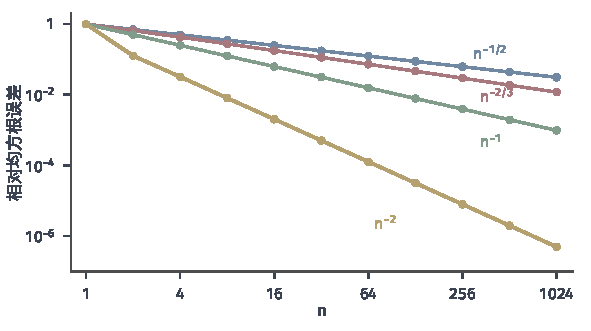
\includegraphics[width=100mm]{figures/07-probability/08-sampling-and-integration/matplotlib/vr-rqmc-rates/figure.pdf}
 \caption{一维等距点随机移位的相对均方根误差$\sqrt{\operatorname{Var}(Q)}/\sigma$，双对数坐标，由$\operatorname{Var}(Q)=n\int_0^{1/n}(Q(\Delta)-I)^2\,\mathrm{d}\Delta$数值积分得到。蓝线为独立抽样$n^{-1/2}$；绿线为$F(u)=\mathrm{e}^{u}$；黄线为帐篷映射后的$\mathrm{e}^{1-\lvert2u-1\rvert}$；红线为Pareto例子的$F(u)=(1-u)^{-1/3}$。}
 \label{fig:vr-rqmc-rates}
\end{BookInlineFigure}

\paragraph{点集与随机化方式}
高维时情况类似，但要同时看点集与随机化方式。格点配合随机移位，对在环面上光滑、Fourier系数衰减快的函数效果最好。另一大类低差异点集称为数字网，它的均匀结构是按二进制位定义的，普通的模$1$平移会破坏这种结构，需要配合按位的随机化，例如随机置乱。已知在被积函数足够光滑时，随机置乱的数字网的均方根误差可以接近$n^{-3/2}$的阶；这一结论的证明较长。无论哪种组合，更快的速度都只在相应的光滑条件下成立。

所以，不能只凭原函数$f$光滑，或者只凭点集差异小，就断言准蒙特卡洛会更准。要检查的是映射后的$F=f\circ T$：它在立方体边界上是否有界、粘起来后是否连续、是否有不沿坐标方向的间断。遇到不利的情形，可以像帐篷映射那样换一个生成映射，或者把奇异部分单独处理；无论效果如何，误差都用整组独立重复来估计。

\subsection{对偶变量}
\label{sec:vr-antithetic}

回到$\int_0^1\mathrm{e}^{u}\,\mathrm{d}u$。$U$与$1-U$都服从$\operatorname{Unif}(0,1)$，而且一个偏大时另一个必然偏小。把它们配成一对，$\mathrm{e}^{U}$偏高的那一次，$\mathrm{e}^{1-U}$就偏低，平均以后偏差部分抵消。

\begin{definition}[对偶变量估计]
\label{def:vr-antithetic}
设$n=2m$，$U_1,\dots,U_m$独立且都服从$\operatorname{Unif}(0,1)$。称
\begin{equation}
 \hat{I}^{\mathrm{anti}}=\frac1m\sum_{i=1}^{m}\frac{F(U_i)+F(1-U_i)}{2}
 \label{eq:vr-antithetic}
\end{equation}
为\term{对偶变量法}（antithetic variates）估计。它用了$n$次函数求值。
\end{definition}

每一对内两点的边缘分布都正确，所以估计无偏。记$\sigma^2=\operatorname{Var}(F(U))$，$\gamma=\operatorname{Cov}(F(U),F(1-U))$。一对的平均的方差为$(\sigma^2+\gamma)/2$，$m$对独立，所以
\begin{equation}
 \operatorname{Var}\bigl(\hat{I}^{\mathrm{anti}}\bigr)=\frac{\sigma^2+\gamma}{2m}=\frac{\sigma^2+\gamma}{n} .
 \label{eq:vr-antithetic-variance}
\end{equation}
同样$n$次求值的独立抽样方差是$\sigma^2/n$。两者相比，对偶变量严格更好当且仅当$\gamma<0$。

\begin{theorem}[单调函数的对偶协方差]
\label{thm:vr-antithetic-monotone}
设$F$在$(0,1)$上单调，$F(U)$平方可积。则$\operatorname{Cov}(F(U),F(1-U))\leq0$。
\end{theorem}

\begin{proof}
不妨设$F$不减。取与$U$独立同分布的$V$。若$U\geq V$，则$F(U)\geq F(V)$，同时$1-U\leq1-V$，$F(1-U)\leq F(1-V)$；$U<V$时两个不等号都反过来。所以
\[
 \bigl(F(U)-F(V)\bigr)\bigl(F(1-U)-F(1-V)\bigr)\leq0 .
\]
展开左边并取期望。由独立性与$1-V\sim\operatorname{Unif}(0,1)$，交叉项的期望都是$I^2$，于是期望等于$2\mathbb{E}[F(U)F(1-U)]-2I^2=2\gamma$，所以$\gamma\leq0$。
\end{proof}

\paragraph{例子与反例}
对$F(u)=\mathrm{e}^{u}$，$F(U)F(1-U)=\mathrm{e}$是常数，
\[
 \gamma=\mathrm{e}-(\mathrm{e}-1)^2\approx-0.23421 .
\]
由式~\eqref{eq:vr-antithetic-variance}，每次求值折合的方差为$\sigma^2+\gamma=0.24204-0.23421=0.00783$，相对效率约为$31$。用$u=0.37$与$0.81$各配一对：
\[
 \tfrac12(\mathrm{e}^{0.37}+\mathrm{e}^{0.63})=1.66267,\qquad \tfrac12(\mathrm{e}^{0.81}+\mathrm{e}^{0.19})=1.72858 ,
\]
平均$1.69563$。

反过来取关于$\tfrac12$对称的$F(u)=(u-\tfrac12)^2$，$I=1/12$。这时$F(1-U)=F(U)$，一对中的两个值完全相同，$\gamma=\sigma^2$，式~\eqref{eq:vr-antithetic-variance}给出$2\sigma^2/n$，是独立抽样的两倍：花了两次求值，只得到一个样本的信息。输入方向相反，本身不保证输出负相关。图~\ref{fig:vr-antithetic}对比了这两种情形。

\begin{BookInlineFigure}
 \centering
 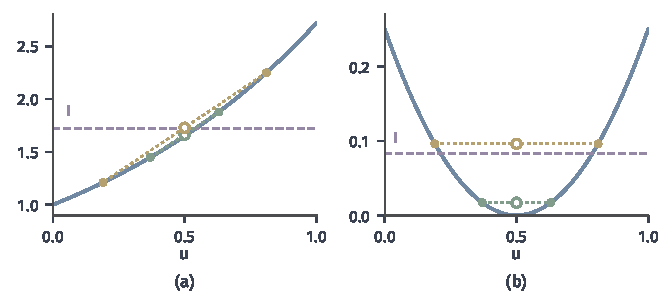
\includegraphics[width=112mm]{figures/07-probability/08-sampling-and-integration/matplotlib/vr-antithetic/figure.pdf}
 \caption{对偶对$(u,1-u)$，$u=0.37$（绿）与$u=0.81$（黄），实心点为两个函数值，$u=\tfrac12$处的空心圆为一对的平均，紫色虚线为积分值$I$。(a)单调的$\mathrm{e}^{u}$：一对的两个值分居$I$两侧，平均接近$I$；(b)对称的$(u-\tfrac12)^2$：一对的两个值相同，平均就是单个值。}
 \label{fig:vr-antithetic}
\end{BookInlineFigure}

\paragraph{奇偶分解}
两个例子可以统一起来。把$F$分成关于$\tfrac12$的偶部与奇部，
\[
 F_{\mathrm{e}}(u)=\frac{F(u)+F(1-u)}{2},\qquad F_{\mathrm{o}}(u)=\frac{F(u)-F(1-u)}{2} .
\]
一对的平均恰好是$F_{\mathrm{e}}(U)$，奇部被完全消去。$F_{\mathrm{e}}F_{\mathrm{o}}$关于$\tfrac12$是奇函数，积分为零，且$\mathbb{E}[F_{\mathrm{o}}(U)]=0$，所以$F_{\mathrm{e}}(U)$与$F_{\mathrm{o}}(U)$不相关，
\[
 \sigma^2=\operatorname{Var}\bigl(F_{\mathrm{e}}(U)\bigr)+\operatorname{Var}\bigl(F_{\mathrm{o}}(U)\bigr) .
\]
于是同样两次求值下，
\[
 \text{对偶一对的方差}=\operatorname{Var}(F_{\mathrm{e}}),\qquad \text{独立两点的方差}=\frac{\operatorname{Var}(F_{\mathrm{e}})+\operatorname{Var}(F_{\mathrm{o}})}{2} .
\]
对偶变量更好，当且仅当奇部的方差大于偶部的方差。单调函数以奇部为主，对称函数只有偶部。在$d$维中把$\bm{U}$换成$\bm{1}-\bm{U}$，对每个坐标都单调的$F$同样有$\gamma\leq0$，这一推广的证明要用到关于单调函数的关联不等式，篇幅较长；奇偶分解的判别对$d$维照样成立，论证与上面相同。

\subsection{共同随机数}
\label{sec:vr-crn}

另一类问题要比较两个方案。设方案A、B的输出分别为随机变量$A$与$B$，要估计期望差$\mathbb{E}[A]-\mathbb{E}[B]$。如果两个方案各自独立抽样，差的估计的方差是两者方差之和；但两个方案往往对同一种随机输入作出相似的反应，若让它们看到同一组随机输入，共同的波动就会在相减时抵消。

\paragraph{方差公式}
设$A=a(\bm{U})$，$B=b(\bm{U})$，$a(\bm{U})$与$b(\bm{U})$分别服从两个方案各自的输出分布。独立生成$\bm{U}_1,\dots,\bm{U}_n$，用
\[
 \hat{\Delta}=\frac1n\sum_{i=1}^{n}\bigl(a(\bm{U}_i)-b(\bm{U}_i)\bigr)
\]
估计$\mathbb{E}[A]-\mathbb{E}[B]$，这种做法称为\term{共同随机数}（common random numbers）。二阶矩有限时，
\begin{equation}
 n\operatorname{Var}(\hat{\Delta})=\operatorname{Var}(A)+\operatorname{Var}(B)-2\operatorname{Cov}(A,B) .
 \label{eq:vr-crn}
\end{equation}
两方案各用$n$个独立输入时，同样$2n$次求值得到的是$\operatorname{Var}(A)+\operatorname{Var}(B)$。所以$\operatorname{Cov}(A,B)>0$时共同随机数严格更好。若$a$与$b$都是同一个标量$U$的不减函数，重复定理~\ref{thm:vr-antithetic-monotone}的证明（这次两个因子同号），可得$\operatorname{Cov}(A,B)\geq0$。

这与对偶变量方向相反。对偶变量要估计一个量的平均，希望同一对中的两个输出负相关；共同随机数要估计两个量的差，希望两个输出正相关。

\paragraph{例子}
两个方案的输出是封顶为$1$的等待时间：$A=\min\{X_A,1\}$，$X_A\sim\operatorname{Exp}(1)$；$B=\min\{X_B,1\}$，$X_B\sim\operatorname{Exp}(1.25)$。都用逆分位数生成，$x=-\ln(1-u)/\lambda$。对非负变量，$\mathbb{E}[\min\{X,1\}]$等于$\mathbb{P}(X>t)$在$[0,1]$上的积分，所以
\[
 \mathbb{E}[A]=1-\mathrm{e}^{-1}=0.63212,\qquad \mathbb{E}[B]=\frac{1-\mathrm{e}^{-1.25}}{1.25}=0.57080 ,
\]
期望差为$0.06132$。数值积分给出$\operatorname{Var}(A)=0.12891$，$\operatorname{Var}(B)=0.12906$，用同一个$u$时$\operatorname{Cov}(A,B)=0.12707$。代入式~\eqref{eq:vr-crn}：
\[
 \begin{aligned}
 \operatorname{Var}(A)+\operatorname{Var}(B)&=0.25796,\\
 \operatorname{Var}(A-B)&=0.25796-2\times0.12707=0.003817 .
 \end{aligned}
\]
差的方差降为$1/67.6$。若不小心让B用$1-u$而A用$u$，两者变成负相关，$\operatorname{Var}(A-B)$升到$0.506$，比独立抽样还差一倍。图~\ref{fig:vr-crn}对比了独立输入与共同输入下的$(A,B)$。

\begin{BookInlineFigure}
 \centering
 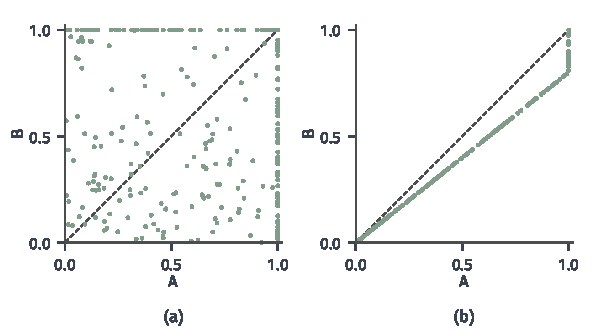
\includegraphics[width=100mm]{figures/07-probability/08-sampling-and-integration/matplotlib/vr-crn/figure.pdf}
 \caption{两个封顶等待时间$A=\min\{X_A,1\}$（$X_A\sim\operatorname{Exp}(1)$）与$B=\min\{X_B,1\}$（$X_B\sim\operatorname{Exp}(1.25)$）的$300$对样本（种子9），虚线为$A=B$。(a)两方案用独立的均匀数；(b)两方案用同一个均匀数，点落在一条递增曲线上，$A-B$的波动很小。}
 \label{fig:vr-crn}
\end{BookInlineFigure}

\paragraph{输入要按用途对齐}
复杂的模拟中，一次运行要消耗许多随机数。要让共同随机数起作用，两个方案应当在同样的用途上使用同一个随机数，例如第$k$个到达时刻都用第$k$个均匀数生成；若某个方案多消耗了一个随机数，后面的所有用途都会错位，协方差随之变小，甚至变号。

\paragraph{有限差分}
共同随机数的一个重要用途是用差商估计导数$\frac{\mathrm{d}}{\mathrm{d}\theta}\mathbb{E}[F(\theta,\bm{U})]$。两个参数值各用独立输入时，差商$\bigl(F(\theta+\delta,\bm{U})-F(\theta,\bm{U}')\bigr)/\delta$的方差约为$2\operatorname{Var}(F)/\delta^2$，$\delta$越小越糟；用同一个$\bm{U}$且$F$对$\theta$光滑时，分子约为$\delta\,\partial_\theta F(\theta,\bm{U})$，差商的方差保持有界。\BookChapterRef{chap:zeroth-order-optimization}{卷五第14章“零阶随机优化”}把这种做法称为共享样本，并分析了它在优化迭代中的作用；含参期望的导数怎样直接用样本表示，由第~\ref{chap:expectation-gradient-estimation}章研究。


\section{本章小结}
\label{sec:vr-summary}

本章固定积分$I=\mathbb{E}_P[f(X)]$，研究怎样在可比的预算下减小随机计算的波动。比较的口径是第~\ref{sec:vr-comparison}节的单元方差乘以单元成本：一种改动只有在$v\,c$变小、而且计入预备成本后仍然划算时才算改进；有偏的估计比较均方误差，并单独检查偏差是否随样本量消失。

三类方法作用在计算流水线的不同位置。改变分布调整重要贡献被抽到的频率：重要性采样按建议分布抽样、乘权重折回，理想建议正比于贡献$\lvert f\rvert p$；它在覆盖条件下无偏，但方差有限要另查加权二阶矩，尾部过轻的建议会使方差为无穷；未知归一化常数时的自归一化估计只是一致的，有限样本有偏，权重的有效样本量看不到漏掉的区域。

改变计算公式消去可以预测或可以精确平均的波动：控制变量减去回归可解释的部分，条件期望把组内波动整个算掉。改变抽样机制控制点的去向与点之间的协方差：分层去掉层间波动，拉丁超立方去掉各坐标的主效应，随机化准蒙特卡洛按Fourier频率过滤误差，对偶变量利用负协方差，共同随机数利用正协方差。

\begin{BookInlineTable}
 \centering
 \caption{本章方法在贯穿例子上的效果。单样本方差均折合到一次函数求值；“倍数”是独立抽样方差与之的比值，未计入额外成本。}
 \label{tab:vr-summary}
 \begin{tabular}{llll}
  \toprule
  方法 & 起作用的条件 & 例子 & 倍数\\
  \midrule
  重要性采样 & $q$接近$\lvert f\rvert p$ & 尾概率，$\lambda=1/4$ & $10.3$\\
  试运行拟合 & 覆盖各区，留防御成分 & 两区域尾部 & $37.7$\\
  控制变量 & $\rho^2$接近$1$ & $\mathrm{e}^{U}$，$h=U$ & $61$\\
  条件期望 & 条件平均可算 & 四分之一圆 & $3.4$\\
  比例分层 & 层均值差别大 & $\mathrm{e}^{U}$，$4$层 & $14.6$\\
  随机移位 & $F$在环面上光滑 & $\mathrm{e}^{U}$，$4$点 & $3.9$\\
  对偶变量 & 奇部方差较大 & $\mathrm{e}^{U}$ & $31$\\
  共同随机数 & 两输出正相关 & 封顶等待时间 & $67.6$\\
  \bottomrule
 \end{tabular}
\end{BookInlineTable}

表~\ref{tab:vr-summary}中的倍数只在各自的例子上成立，并且每一行都有反例：$\lambda\geq2$的指数建议、没有防御成分的拟合、交互型函数上的拉丁超立方、对称函数上的对偶对、用反向输入的共同随机数，都会使方差不降反升甚至为无穷。生成映射$T$也会改变结论，同一个光滑的$f$经过不同的$T$，随机化准蒙特卡洛的误差速度可以从$n^{-2}$降到$n^{-2/3}$。

样本不再独立时，误差估计要相应改变：整组随机化的方法以完整的一组为独立单位，用组间方差除以重复次数估计误差，不能用组内点的样本方差代替。三类操作可以组合，例如在拉丁超立方的点上再用控制变量，或在分层的每层内用重要性采样；但期望正确、方差有限与节省总计算量是三个不同的要求，组合后要重新逐项检查，各方法单独使用时的改进不能直接相乘。实际预算下怎样分配试运行与正式计算、怎样在方法之间取舍，由第~\ref{chap:sampling-budget-method-selection}章统一讨论；下一章把同样的思路用于含参期望的梯度。


\chapter{含参期望的梯度估计}
\label{chap:expectation-gradient-estimation}

设$X\sim\mathcal{N}(\theta,1)$，要计算$J(\theta)=\mathbb{E}[X^{2}]$对$\theta$的导数。这个例子有闭式答案$J(\theta)=\theta^{2}+1$，导数是$2\theta$。可是一旦分布或函数稍复杂，期望本身就只能用样本平均近似，导数也只能靠样本来算。一个自然的想法是把样本平均$\frac{1}{n}\sum_{i}X_{i}^{2}$对$\theta$求导；但$X_{i}^{2}$的表达式里看不到$\theta$，这样求出的导数是零。错在哪里？参数没有出现在函数里，却改变了样本从哪里来。

本章研究这类问题：含参期望$J(\bm{\theta})$等于$\mathbb{E}_{\bm{\theta}}[f_{\bm{\theta}}(X)]$，其中的参数既可能改变被积函数，也可能改变概率分布，怎样用随机样本计算$\nabla J(\bm{\theta})$，所得的估计在什么条件下无偏、方差有多大。第一步是看清参数从哪里进入期望，并把“导数能否移到期望里面”这件事化为一个可检验的控制条件。之后按参数进入的位置分三种处理：分布固定时直接对函数求导；分布可以写成固定噪声经过含参映射的结果时，沿样本的生成路径求导（重参数化）；两者都不方便时，对概率权重求导（得分函数估计），包括归一化常数未知的情形。

三种表示的期望相同，样本上的波动却可以相差很多，因此接着用第~\ref{chap:variance-reduction}章的控制变量与条件期望来降低梯度估计的方差。最后讨论样本来自近似生成器或有限步Markov链时，求出的到底是谁的梯度。全章反复使用开头的高斯例子：$X=\theta+\varepsilon$、$\varepsilon\sim\mathcal{N}(0,1)$、$f(x)=x^{2}$，手算时固定四个标准正态数$\varepsilon=0.3,-1.1,0.8,-0.4$，读者可以逐步复现。

\section{含参期望}
\label{sec:pgrad-parametric}

参数$\bm{\theta}\in\Theta\subseteq\mathbb{R}^{k}$对应一族概率分布$P_{\bm{\theta}}$和一族被积函数$f_{\bm{\theta}}$，记
\begin{equation}
  J(\bm{\theta})=\mathbb{E}_{\bm{\theta}}[f_{\bm{\theta}}(X)]=\int f_{\bm{\theta}}(x)\,P_{\bm{\theta}}(\mathrm{d}x),
  \label{eq:pgrad-J}
\end{equation}
其中$\mathbb{E}_{\bm{\theta}}$表示$X\sim P_{\bm{\theta}}$时的期望。称这样的$J$为\term{含参期望}（parameter-dependent expectation）。目标是用样本计算梯度$\nabla J(\bm{\theta})\in\mathbb{R}^{k}$。在动手构造估计之前，有两件事要先弄清：参数改变了期望里的哪些量，以及什么时候允许把求导移进期望。

\paragraph{参数进入期望的位置}

计算期望要做三件事：按某种规律产生样本，在样本处求函数值，再按概率加权平均。参数可以在其中任何一处起作用。图~\ref{fig:pgrad-three-entries}把三种位置并排画出。

\begin{BookInlineFigure}
  \centering
  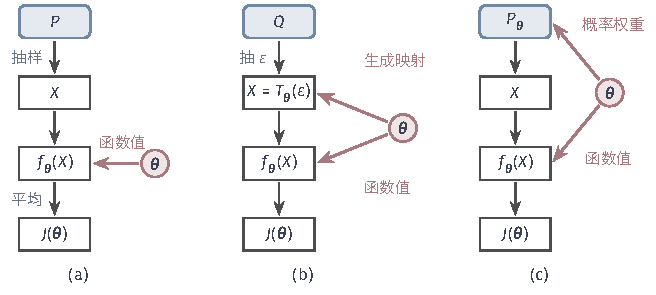
\includegraphics[width=111mm]{figures/07-probability/08-sampling-and-integration/tikz/pgrad-three-entries/figure.pdf}
  \caption{参数进入含参期望的三个位置。每列自上而下是随机性的来源、样本、函数值和期望；红色圆点标出参数进入之处。(a)抽样分布$P$固定，参数只改变函数值；(b)样本由固定分布$Q$的噪声$\varepsilon$经含参映射$T_{\bm{\theta}}$生成，参数既改变生成映射也改变函数；(c)参数改变分布$P_{\bm{\theta}}$本身，即改变各处的概率权重，同时也可以改变函数。}
  \label{fig:pgrad-three-entries}
\end{BookInlineFigure}

第一处是函数值：$f_{\bm{\theta}}(x)$在同一个$x$上随$\bm{\theta}$改变。第二处是概率权重：若$P_{\bm{\theta}}$有相对某个固定参考测度$\nu$的密度$p_{\bm{\theta}}$，参数改变的是各位置上的密度，即质量怎样分配。第三处是生成映射：样本写成$X=T_{\bm{\theta}}(\varepsilon)$，噪声$\varepsilon$的分布不变，参数改变的是同一个$\varepsilon$被送到哪里。

后两处描述的是同一件事的两种看法。对$X\sim\mathcal{N}(\theta,1)$，可以说“密度$p_{\theta}(x)=\varphi(x-\theta)$随$\theta$平移”，也可以说“$X=\theta+\varepsilon$，每个样本都向右挪了一段”。两种说法给出同一个分布族，计算梯度时只选一种，不能把分布的变化算两次。真正的要求是：在选定的表示里，凡是实际随参数变化的项都要计入，一项也不能漏。

\paragraph{两项相互抵消的例子}

取$X\sim\mathcal{N}(\theta,1)$与$f_{\theta}(x)=x^{2}-\theta x$。由$\mathbb{E}_{\theta}[X]=\theta$与$\mathbb{E}_{\theta}[X^{2}]=\theta^{2}+1$，得到
\[
  J(\theta)=\theta^{2}+1-\theta\cdot\theta=1 .
\]
$J$是常数，导数为零。现在把两种变化分开。固定分布在$\theta_{0}$，只让函数里的参数变成$t$，期望是
\[
  A(t)=\mathbb{E}_{\theta_{0}}[X^{2}-tX]=\theta_{0}^{2}+1-t\theta_{0},
\]
它在$t=\theta_{0}$处的斜率是$-\theta_{0}$。反过来固定函数为$f_{\theta_{0}}$，只让分布的参数变成$t$，期望是
\[
  B(t)=\mathbb{E}_{t}[X^{2}-\theta_{0}X]=t^{2}+1-\theta_{0}t,
\]
它在$t=\theta_{0}$处的斜率是$2\theta_{0}-\theta_{0}=\theta_{0}$。

两个斜率相加为零，正是$J'(\theta_{0})$。这就是二元函数$H(t_{1},t_{2})=\mathbb{E}_{t_{2}}[f_{t_{1}}(X)]$沿对角线$J(\theta)=H(\theta,\theta)$求导的链式法则（$H$在这里是多项式，可微性没有问题）。图~\ref{fig:pgrad-two-terms}在$\theta_{0}=1$处画出了三条曲线。只对函数求导会得到$-1$，只对分布求导会得到$+1$，两者都不是答案。

\begin{BookInlineFigure}
  \centering
  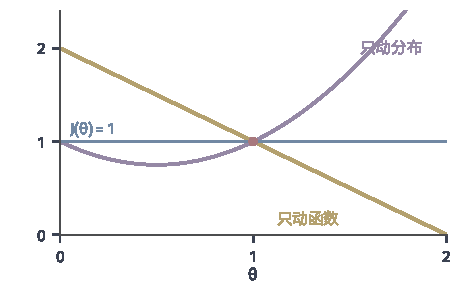
\includegraphics[width=78mm]{figures/07-probability/08-sampling-and-integration/matplotlib/pgrad-two-terms/figure.pdf}
  \caption{$X\sim\mathcal{N}(\theta,1)$，$f_{\theta}(x)=x^{2}-\theta x$。蓝线为$J(\theta)=1$；黄线为只让函数中的参数变化的$A(\theta)$；紫线为只让分布的参数变化的$B(\theta)$。三条线在红点$\theta=1$处相交，黄线斜率$-1$与紫线斜率$+1$之和等于蓝线斜率$0$。}
  \label{fig:pgrad-two-terms}
\end{BookInlineFigure}

\paragraph{期望在哪里有定义}

$J(\bm{\theta})$首先要有意义，即$f_{\bm{\theta}}$在$P_{\bm{\theta}}$下可积。例如$X\sim\operatorname{Exp}(1)$、$f_{\theta}(x)=\mathrm{e}^{\theta x}$时，
\[
  J(\theta)=\int_{0}^{\infty}\mathrm{e}^{\theta x}\mathrm{e}^{-x}\,\mathrm{d}x=\frac{1}{1-\theta},\qquad \theta<1,
\]
而$\theta\geq1$时积分发散。导数只在使$J$有定义的参数构成的开集内讨论：在某点求导，要求从该点出发朝每个方向走一小步，期望仍然有定义。因此下面总取一个以$\bm{\theta}_{0}$为中心、含在$\Theta$内的开球$U$，并检查$U$中每个参数下的可积性，而不只看$\bm{\theta}_{0}$这一点。

\paragraph{统一成固定测度上的积分}

三种参数位置可以写成同一种形式。图~\ref{fig:pgrad-three-entries}的三列分别对应
\[
  J(\bm{\theta})=\int f_{\bm{\theta}}\,\mathrm{d}P,\quad
  J(\bm{\theta})=\int f_{\bm{\theta}}(T_{\bm{\theta}}(\varepsilon))\,Q(\mathrm{d}\varepsilon),\quad
  J(\bm{\theta})=\int f_{\bm{\theta}}\,p_{\bm{\theta}}\,\mathrm{d}\nu .
\]
三个积分所对的测度$P$、$Q$、$\nu$都不随参数变化，参数全部被移进了被积函数。于是问题都化为：测度$\mu$固定，$g(\bm{\theta},x)$含参，
\begin{equation}
  J(\bm{\theta})=\int g(\bm{\theta},x)\,\mu(\mathrm{d}x)
  \label{eq:pgrad-fixed-measure}
\end{equation}
的梯度能否写成$\int\nabla_{\bm{\theta}}g(\bm{\theta},x)\,\mu(\mathrm{d}x)$。后面三节的区别只在于选哪个$\mu$和$g$，交换条件都由下面的定理检查。

\paragraph{交换的条件}

逐点可微只说明每个$x$上的函数$\bm{\theta}\mapsto g(\bm{\theta},x)$光滑，并不说明这些变化积分起来仍然受控：变化可能集中在越来越小的区域上，每个固定点都“看不到”它。需要一个与参数无关、可积的函数控制所有差商。

\begin{theorem}[积分号下求导]
\label{thm:pgrad-exchange}
设$\mu$是可测空间$\mathcal{X}$上的测度，$\bm{\theta}_{0}\in\Theta$，$U\subseteq\Theta$是以$\bm{\theta}_{0}$为中心的开球。设$g:U\times\mathcal{X}\to\mathbb{R}$满足：
\begin{enumerate}
  \item 对每个$\bm{\theta}\in U$，$g(\bm{\theta},\cdot)$可测，且$g(\bm{\theta}_{0},\cdot)$关于$\mu$可积；
  \item 对$\mu$几乎所有$x$，$\bm{\theta}\mapsto g(\bm{\theta},x)$在$\bm{\theta}_{0}$处可微；
  \item 存在$\mu$可积的函数$M\geq0$，使对$\mu$几乎所有$x$及所有$\bm{\theta},\bm{\theta}'\in U$，
  \begin{equation}
    \lvert g(\bm{\theta},x)-g(\bm{\theta}',x)\rvert\leq M(x)\lVert\bm{\theta}-\bm{\theta}'\rVert_{2}.
    \label{eq:pgrad-lipschitz}
  \end{equation}
\end{enumerate}
则对每个$\bm{\theta}\in U$，$g(\bm{\theta},\cdot)$可积，$\nabla_{\bm{\theta}}g(\bm{\theta}_{0},\cdot)$可积，式~\eqref{eq:pgrad-fixed-measure}的$J$在$\bm{\theta}_{0}$处可微，并且
\begin{equation}
  \nabla J(\bm{\theta}_{0})=\int\nabla_{\bm{\theta}}g(\bm{\theta}_{0},x)\,\mu(\mathrm{d}x).
  \label{eq:pgrad-exchange}
\end{equation}
\end{theorem}

\begin{proof}
先看可积性。由式~\eqref{eq:pgrad-lipschitz}取$\bm{\theta}'=\bm{\theta}_{0}$，对几乎所有$x$有
\[
  \lvert g(\bm{\theta},x)\rvert\leq\lvert g(\bm{\theta}_{0},x)\rvert+M(x)\lVert\bm{\theta}-\bm{\theta}_{0}\rVert_{2},
\]
右边可积，所以$g(\bm{\theta},\cdot)$可积，$J$在$U$上有定义。

再看梯度本身。记$\bm{v}(x)$为$g(\cdot,x)$在$\bm{\theta}_{0}$处的梯度，它的第$j$个分量是差商$\bigl(g(\bm{\theta}_{0}+h\bm{e}_{j},x)-g(\bm{\theta}_{0},x)\bigr)/h$沿$h=1/m\to0$的极限，是可测函数的极限，因而可测。由式~\eqref{eq:pgrad-lipschitz}，这些差商的绝对值都不超过$M(x)$，所以
\[
  \lVert\bm{v}(x)\rVert_{2}\leq\sqrt{k}\,M(x),
\]
$\bm{v}$可积。

最后证明可微。任取$\bm{h}_{m}\to\bm{0}$，$\bm{h}_{m}\neq\bm{0}$，$\bm{\theta}_{0}+\bm{h}_{m}\in U$，令
\[
  R_{m}(x)=\frac{g(\bm{\theta}_{0}+\bm{h}_{m},x)-g(\bm{\theta}_{0},x)-\langle\bm{v}(x),\bm{h}_{m}\rangle}{\lVert\bm{h}_{m}\rVert_{2}}.
\]
由条件2，对几乎所有$x$有$R_{m}(x)\to0$。由式~\eqref{eq:pgrad-lipschitz}与上一步的界，
\[
  \lvert R_{m}(x)\rvert\leq M(x)+\lVert\bm{v}(x)\rVert_{2}\leq(1+\sqrt{k})M(x).
\]
控制收敛定理给出$\int R_{m}\,\mathrm{d}\mu\to0$，也就是
\[
  \frac{J(\bm{\theta}_{0}+\bm{h}_{m})-J(\bm{\theta}_{0})-\bigl\langle\int\bm{v}\,\mathrm{d}\mu,\bm{h}_{m}\bigr\rangle}{\lVert\bm{h}_{m}\rVert_{2}}\to0 .
\]
序列$\bm{h}_{m}$是任取的，这正是$J$在$\bm{\theta}_{0}$处可微且梯度为$\int\bm{v}\,\mathrm{d}\mu$的定义。
\end{proof}

控制收敛定理的条件与证明可参考\BookChapterRef{chap:integration}{卷四第6章“积分”}。三个条件各管一件事。开球保证可以朝任意方向走一小步，并且沿线段比较。条件2只要求在$\bm{\theta}_{0}$这一点可微，例如$g(\theta,x)=\lvert\theta+x\rvert$在$\theta+x=0$处不可微，但对固定的$\theta_{0}$，这样的$x$只有一个，只要$\mu$在这一点没有质量，就不影响结论。条件3是关键：常数$M(x)$不能依赖参数，而且要对$x$可积。

常用的充分条件是梯度的一致控制。若对几乎所有$x$，$g(\cdot,x)$在整个$U$上可微，并且
\[
  \sup_{\bm{\theta}\in U}\lVert\nabla_{\bm{\theta}}g(\bm{\theta},x)\rVert_{2}\leq M(x),
\]
则沿连接$\bm{\theta}'$与$\bm{\theta}$的线段用中值定理，即得式~\eqref{eq:pgrad-lipschitz}。高斯族里的多项式函数就适合这样检查：参数限制在有界球内时，梯度不超过某个多项式乘以$\mathrm{e}^{-cx^{2}}$，后者可积。

\paragraph{逐点可微而交换失败}

下面的例子说明条件3不能省。取$U\sim\operatorname{Unif}(0,1)$，对$u\in(0,1)$令
\[
  g(\theta,u)=\frac{2\theta^{3}u}{(u^{2}+\theta^{2})^{2}},\qquad g(0,u)=0 .
\]
对每个固定的$u>0$，$g(\cdot,u)$是$\theta$的光滑函数。在$\theta=0$处，差商
\[
  \frac{g(\theta,u)-g(0,u)}{\theta}=\frac{2\theta^{2}u}{(u^{2}+\theta^{2})^{2}}\to0\qquad(\theta\to0),
\]
所以逐点导数为零，积分后仍是零。

另一方面，令$w=u^{2}+\theta^{2}$，$\mathrm{d}w=2u\,\mathrm{d}u$，对$\theta\neq0$有
\[
  J(\theta)=\theta^{3}\int_{\theta^{2}}^{1+\theta^{2}}w^{-2}\,\mathrm{d}w=\theta^{3}\Bigl(\frac{1}{\theta^{2}}-\frac{1}{1+\theta^{2}}\Bigr)=\frac{\theta}{1+\theta^{2}} .
\]
这个式子在$\theta=0$也成立，于是$J'(0)=1\neq0$。

失败的原因在图~\ref{fig:pgrad-moving-spike}(a)中一目了然。$g(\theta,\cdot)$是一个高度固定（约$0.65$）、宽度与$\theta$成正比的尖峰，$\theta\to0$时它被挤向$u=0$，面积约为$\theta$。每个固定的$u$最终都落在尖峰右侧，只看到函数值趋于零；尖峰携带的面积却以斜率$1$消失。用定理的语言说：对$\theta$求偏导数，
\[
  \partial_{\theta}g(\theta,u)=\frac{2u\bigl(3\theta^{2}(u^{2}+\theta^{2})-4\theta^{4}\bigr)}{(u^{2}+\theta^{2})^{3}},
\]
在$\theta=u$处它等于$1/(2u)$。任何满足式~\eqref{eq:pgrad-lipschitz}的$M$都要在$(0,\delta)$上不小于$1/(2u)$，而$\int_{0}^{\delta}\frac{1}{2u}\,\mathrm{d}u=\infty$。被积函数本身有界、逐点光滑，仍然不够。

\begin{BookInlineFigure}
  \centering
  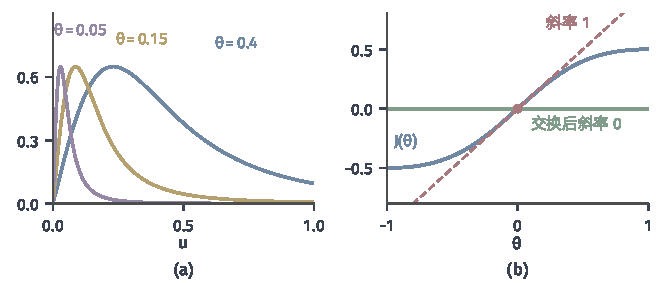
\includegraphics[width=112mm]{figures/07-probability/08-sampling-and-integration/matplotlib/pgrad-moving-spike/figure.pdf}
  \caption{逐点可微而不能交换求导与积分。(a)$g(\theta,u)=2\theta^{3}u/(u^{2}+\theta^{2})^{2}$在$\theta=0.4,0.15,0.05$时的图像，峰高都约为$0.65$，峰向$u=0$移动并变窄。(b)蓝线为$J(\theta)=\theta/(1+\theta^{2})$，红色虚线是它在原点处斜率为$1$的切线，绿线是逐点求导后再积分得到的斜率$0$。}
  \label{fig:pgrad-moving-spike}
\end{BookInlineFigure}

这个例子也说明了为什么检查要放在参数的一个邻域上，而不只在$\bm{\theta}_{0}$：在$\theta=0$这一点，每个$u$处的导数都存在且有界，毛病出在$\theta$离开零的过程中。后面每种梯度表示都先写成式~\eqref{eq:pgrad-fixed-measure}的形式，再用定理~\ref{thm:pgrad-exchange}检查。

\section{固定分布下的直接求导}
\label{sec:pgrad-direct}

最简单的情形是图~\ref{fig:pgrad-three-entries}(a)：抽样分布$P$与参数无关，参数只出现在函数里，$J(\bm{\theta})=\mathbb{E}_{P}[f_{\bm{\theta}}(X)]$。这时可以先在每个样本处对函数求导，再取平均吗？

\paragraph{梯度表示}

在定理~\ref{thm:pgrad-exchange}中取$\mu=P$、$g(\bm{\theta},x)=f_{\bm{\theta}}(x)$。若$f_{\bm{\theta}_{0}}$在$P$下可积，对$P$几乎所有$x$在$\bm{\theta}_{0}$处可微，并且在$\bm{\theta}_{0}$的某个开球$U$上满足式~\eqref{eq:pgrad-lipschitz}的可积控制，则
\begin{equation}
  \nabla J(\bm{\theta})=\mathbb{E}_{P}\bigl[\nabla_{\bm{\theta}}f_{\bm{\theta}}(X)\bigr].
  \label{eq:pgrad-direct}
\end{equation}
梯度本身成了一个期望，被积函数是逐样本的导数$\bm{G}=\nabla_{\bm{\theta}}f_{\bm{\theta}}(X)$。卷五的随机梯度方法就是在这种情形下使用样本梯度的，相应的交换引理可参考\BookChapterRef{chap:stochastic-gradient-methods}{卷五第13章“随机梯度方法”}。

\paragraph{样本估计}

取$X_{1},\dots,X_{n}$独立同分布于$P$，令
\begin{equation}
  \hat{\bm{g}}_{n}^{\mathrm{dir}}=\frac{1}{n}\sum_{i=1}^{n}\nabla_{\bm{\theta}}f_{\bm{\theta}}(X_{i}).
  \label{eq:pgrad-direct-estimator}
\end{equation}
这就是第~\ref{chap:monte-carlo-integration-error}章的样本平均，只不过被平均的是一个$\mathbb{R}^{k}$值函数。对它要问两件事，所需的条件不同。

第一件是期望与一致性。定理~\ref{thm:pgrad-exchange}的证明已经给出$\lVert\bm{G}\rVert_{2}\leq\sqrt{k}M(X)$，所以$\bm{G}$可积。由期望的线性，$\hat{\bm{g}}_{n}^{\mathrm{dir}}$的期望就是$\nabla J(\bm{\theta})$，估计无偏；对每个分量用强大数律（第~\ref{chap:laws-of-large-numbers}章），$\hat{\bm{g}}_{n}^{\mathrm{dir}}$几乎必然收敛到$\nabla J(\bm{\theta})$。这两条只用到一阶矩。

第二件是误差的大小。若$\mathbb{E}\lVert\bm{G}\rVert_{2}^{2}<\infty$，记$\bm{G}$的协方差矩阵为$\bm{\Sigma}_{\bm{G}}$，则各分量独立同分布平均的方差是$(\bm{\Sigma}_{\bm{G}})_{j,j}/n$，相加得到均方误差
\begin{equation}
  \mathbb{E}\bigl\lVert\hat{\bm{g}}_{n}^{\mathrm{dir}}-\nabla J(\bm{\theta})\bigr\rVert_{2}^{2}=\frac{\operatorname{tr}\bm{\Sigma}_{\bm{G}}}{n}.
  \label{eq:pgrad-direct-mse}
\end{equation}
这是熟悉的$n^{-1/2}$误差尺度。没有二阶矩时上式右边是无穷，大数律仍然成立，但误差缩小的速度可以慢得多。导数的可积性支撑“算得对”，导数的平方可积性才支撑“算得多准”。

\paragraph{一个只有一阶矩的例子}

设$X$的密度为$3x^{-4}$（$x\geq1$），$f_{\theta}(x)=x^{\theta}$。对$\theta<3$，
\[
  J(\theta)=\int_{1}^{\infty}x^{\theta}\cdot3x^{-4}\,\mathrm{d}x=\frac{3}{3-\theta},
\]
$\theta\geq3$时积分发散，所以只在$\theta<3$上讨论。逐样本导数是$G=X^{\theta}\ln X$。

先检查交换条件。取$\delta>0$使$\theta+\delta<3$，在$U=(\theta-\delta,\theta+\delta)$上
\[
  \bigl\lvert\partial_{\theta'}x^{\theta'}\bigr\rvert=x^{\theta'}\ln x\leq x^{\theta+\delta}\ln x,\qquad x\geq1,
\]
右边在$X$的分布下可积，因为
\[
  \int_{1}^{\infty}x^{\theta+\delta}\ln x\cdot3x^{-4}\,\mathrm{d}x=\frac{3}{(3-\theta-\delta)^{2}}<\infty .
\]于是由式~\eqref{eq:pgrad-direct}，
\[
  J'(\theta)=\mathbb{E}[X^{\theta}\ln X]=\frac{3}{(3-\theta)^{2}},
\]
与直接对$3/(3-\theta)$求导一致。

再看二阶矩。分部积分两次可得，对$a>1$，
\[
  \int_{1}^{\infty}x^{-a}\ln^{2}x\,\mathrm{d}x=\frac{2}{(a-1)^{3}} .
\]
取$a=4-2\theta$，得到
\[
  \mathbb{E}[G^{2}]=3\int_{1}^{\infty}x^{2\theta-4}\ln^{2}x\,\mathrm{d}x=\frac{6}{(3-2\theta)^{3}},\qquad\theta<\tfrac{3}{2},
\]
$\theta\geq\frac{3}{2}$时为无穷。在$\theta=1$处$J'(1)=\frac{3}{4}$，$\mathbb{E}[G^{2}]=6$，单样本方差$6-\frac{9}{16}=\frac{87}{16}\approx5.44$。在$\theta=2$处$J'(2)=3$，导数可积而方差无穷。

手算时用逆变换采样（第~\ref{chap:sample-generation}章）：分布函数是$1-x^{-3}$，于是$X=(1-U)^{-1/3}$。取均匀数$u=0.37,0.80,0.15,0.62$，得
\[
  X=1.1665,\ 1.7100,\ 1.0557,\ 1.3806 .
\]
在$\theta=1$处，四个导数样本$G=X\ln X$是
\[
  G=0.1797,\ 0.9174,\ 0.0572,\ 0.4453,
\]
平均为$0.3999$，真值是$0.75$。偏离约$0.35$，而四样本平均的标准差是$\sqrt{5.44/4}\approx1.17$，这个偏离在正常波动范围内。

图~\ref{fig:pgrad-pareto-paths}把样本数加到两万。$\theta=1$时各条路径在几百个样本后就贴近真值；$\theta=2$时路径长时间偏低，偶尔被一个巨大的样本拉高，然后再缓慢回落。这是无穷方差下的典型样子：绝大多数样本偏小，期望里相当一部分来自稀少的大值。

\begin{BookInlineFigure}
  \centering
  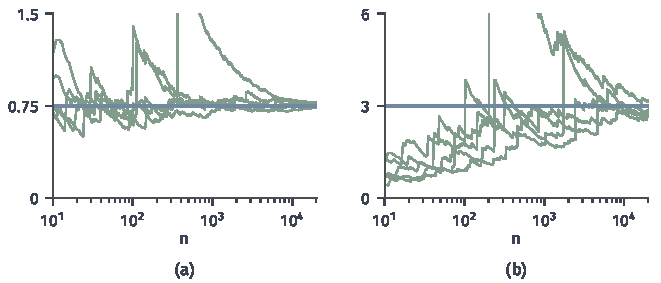
\includegraphics[width=112mm]{figures/07-probability/08-sampling-and-integration/matplotlib/pgrad-pareto-paths/figure.pdf}
  \caption{密度为$3x^{-4}$（$x\geq1$）时，导数样本$X^{\theta}\ln X$的运行平均，横轴为样本数$n$（对数刻度）。绿线为五条固定种子的独立路径，蓝线为真值$J'(\theta)=3/(3-\theta)^{2}$。(a)$\theta=1$，导数有有限方差；(b)$\theta=2$，导数可积但方差无穷。}
  \label{fig:pgrad-pareto-paths}
\end{BookInlineFigure}

图~\ref{fig:pgrad-pareto-error}量化了这种差别。对每个$n$重复$2000$次，取估计误差绝对值的中位数。$\theta=1$时误差沿$n^{-1/2}$的斜率下降，与式~\eqref{eq:pgrad-direct-mse}一致；$\theta=2$时下降明显更慢。这里$G$的尾部满足$\mathbb{P}(G>t)$约按$t^{-3/2}$（差一个对数因子）衰减，这类平均的误差尺度大约是$n^{-1/3}$。这一尺度来自重尾独立和的稳定极限，证明要用较细的特征函数估计，篇幅较长，读者可查阅~\scite{math-kallenberg2021probability}。图中$\theta=2$的折线在所示范围内甚至比这条参考线还平，对数因子在小样本时尤其明显。

\begin{BookInlineFigure}
  \centering
  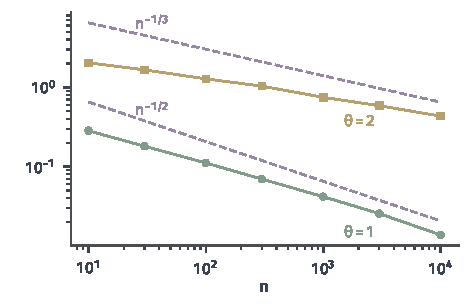
\includegraphics[width=80mm]{figures/07-probability/08-sampling-and-integration/matplotlib/pgrad-pareto-error/figure.pdf}
  \caption{同一例子中，$n$个导数样本平均的误差绝对值的中位数（每个$n$重复$2000$次，固定种子），双对数坐标。绿色圆点为$\theta=1$，黄色方块为$\theta=2$；紫色虚线是斜率为$-1/2$与$-1/3$的参考线。}
  \label{fig:pgrad-pareto-error}
\end{BookInlineFigure}

这个例子的教训适用于本章所有梯度估计：先用局部控制确认梯度可以写成期望，再单独检查梯度样本的二阶矩，二者不能互相代替。参数离可积性边界越近，导数样本的尾部越重，即使期望仍然有限，样本估计也会变得不可靠。

\section{重参数化估计}
\label{sec:pgrad-reparam}

回到章首的问题：$X\sim\mathcal{N}(\theta,1)$，$J(\theta)=\mathbb{E}[X^{2}]$。参数改变的是分布，上一节的方法不能直接用。但第~\ref{chap:sample-generation}章的生成方法提示了另一种写法：先抽$\varepsilon\sim\mathcal{N}(0,1)$，再令$X=\theta+\varepsilon$。噪声的分布与$\theta$无关，参数只出现在这个确定的映射里，于是分布的变化被改写成了函数的变化。

\paragraph{生成映射与梯度表示}

一般地，设噪声$\varepsilon$取值于某个空间、分布为$Q$且不依赖参数，$T_{\bm{\theta}}$是从噪声到$\mathbb{R}^{d}$的映射，使$T_{\bm{\theta}}(\varepsilon)$的分布正是$P_{\bm{\theta}}$，即$P_{\bm{\theta}}$是$Q$在$T_{\bm{\theta}}$下的推前。这样的写法称为\term{重参数化}（reparameterization）。由推前的换元公式，
\begin{equation}
  J(\bm{\theta})=\mathbb{E}_{Q}\bigl[f_{\bm{\theta}}(T_{\bm{\theta}}(\varepsilon))\bigr].
  \label{eq:pgrad-reparam-J}
\end{equation}
期望所对的分布$Q$固定，形式上回到了上一节：在定理~\ref{thm:pgrad-exchange}中取$\mu=Q$，以式~\eqref{eq:pgrad-reparam-J}方括号内的复合函数作$g(\bm{\theta},\varepsilon)$即可。

对固定的$\varepsilon$求$g$对$\bm{\theta}$的导数，要用链式法则。设$f_{\bm{\theta}}(x)$对$(\bm{\theta},x)$连续可微，$T_{\bm{\theta}}(\varepsilon)$对$\bm{\theta}$可微，记$x=T_{\bm{\theta}}(\varepsilon)$，$D_{\bm{\theta}}T_{\bm{\theta}}(\varepsilon)$为$d\times k$的Jacobi矩阵。参数沿两条路到达函数值：一条直接进入$f_{\bm{\theta}}$，另一条先移动样本点$x$，再经$f_{\bm{\theta}}$对$x$的梯度传到函数值。两条路的贡献相加，
\begin{equation}
  \nabla_{\bm{\theta}}\bigl[f_{\bm{\theta}}(T_{\bm{\theta}}(\varepsilon))\bigr]
  =\nabla_{\bm{\theta}}f_{\bm{\theta}}(x)+\bigl(D_{\bm{\theta}}T_{\bm{\theta}}(\varepsilon)\bigr)^{\top}\nabla_{x}f_{\bm{\theta}}(x).
  \label{eq:pgrad-chain}
\end{equation}
图~\ref{fig:pgrad-chain-paths}画出这两条路。称它为沿样本生成路径的导数，即\term{路径导数}（pathwise derivative）。

\begin{BookInlineFigure}
  \centering
  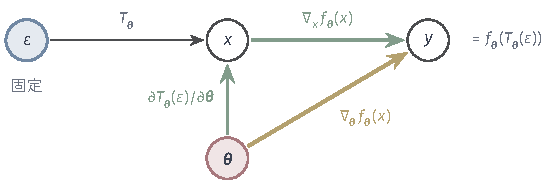
\includegraphics[width=94mm]{figures/07-probability/08-sampling-and-integration/tikz/pgrad-chain-paths/figure.pdf}
  \caption{一个重参数化样本的计算图。噪声$\varepsilon$（蓝）固定，参数$\bm{\theta}$（红）经两条路影响函数值$y$：黄色箭头是函数自身对参数的导数，绿色箭头是先经生成映射移动样本点、再经函数对$x$的梯度传递的部分。路径导数是两部分之和。}
  \label{fig:pgrad-chain-paths}
\end{BookInlineFigure}

把这些条件合起来，就得到重参数化的梯度表示。

\begin{theorem}[重参数化梯度]
\label{thm:pgrad-reparam}
设$P_{\bm{\theta}}$是$Q$在$T_{\bm{\theta}}$下的推前，$U$是以$\bm{\theta}_{0}$为中心的开球，复合函数$g(\bm{\theta},\varepsilon)$等于$f_{\bm{\theta}}(T_{\bm{\theta}}(\varepsilon))$。设对$Q$几乎所有$\varepsilon$，$\bm{\theta}\mapsto T_{\bm{\theta}}(\varepsilon)$在$\bm{\theta}_{0}$处可微，$(\bm{\theta},x)\mapsto f_{\bm{\theta}}(x)$在$(\bm{\theta}_{0},T_{\bm{\theta}_{0}}(\varepsilon))$的某个邻域内连续可微；又设$g$满足定理~\ref{thm:pgrad-exchange}的条件1与条件3（取$\mu=Q$）。记$X=T_{\bm{\theta}_{0}}(\varepsilon)$，则
\begin{equation}
  \nabla J(\bm{\theta}_{0})=\mathbb{E}_{Q}\Bigl[\nabla_{\bm{\theta}}f_{\bm{\theta}_{0}}(X)+\bigl(D_{\bm{\theta}}T_{\bm{\theta}_{0}}(\varepsilon)\bigr)^{\top}\nabla_{x}f_{\bm{\theta}_{0}}(X)\Bigr].
  \label{eq:pgrad-reparam}
\end{equation}
\end{theorem}

证明就是定理~\ref{thm:pgrad-exchange}本身。所设的可微性使链式法则对几乎所有$\varepsilon$成立，于是$g(\cdot,\varepsilon)$在$\bm{\theta}_{0}$处可微，梯度由式~\eqref{eq:pgrad-chain}给出，这正是定理~\ref{thm:pgrad-exchange}的条件2；再由式~\eqref{eq:pgrad-exchange}，$J$的梯度等于这些逐点梯度关于$Q$的积分。对独立的$\varepsilon_{1},\dots,\varepsilon_{n}\sim Q$，令$X_{i}=T_{\bm{\theta}}(\varepsilon_{i})$，\term{重参数化估计}（reparameterization gradient estimator）是式~\eqref{eq:pgrad-reparam}方括号内的量在这$n$个样本上的平均，记作$\hat{\bm{g}}_{n}^{\mathrm{rep}}$。无偏性、一致性与均方误差的讨论与上一节完全相同。

\paragraph{高斯的平移与尺度}

最常用的生成映射是高斯的位置尺度变换$X=\mu+\sigma\varepsilon$，$\varepsilon\sim\mathcal{N}(0,1)$，参数$\bm{\theta}=(\mu,\sigma)$，$\sigma>0$。映射对参数的导数是
\[
  \frac{\partial X}{\partial\mu}=1,\qquad\frac{\partial X}{\partial\sigma}=\varepsilon .
\]
增大$\mu$时每个样本平移同样的距离；增大$\sigma$时每个样本沿远离$\mu$的方向移动，移动量与它的$\varepsilon$成正比，$\varepsilon$为负的样本向左走，为正的向右走。图~\ref{fig:pgrad-reparam-map}用四个固定的$\varepsilon$画出了这两种移动。

\begin{BookInlineFigure}
  \centering
  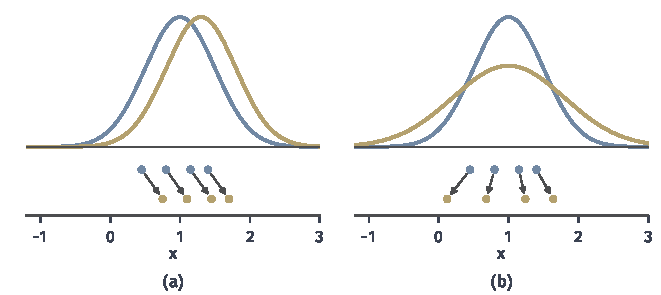
\includegraphics[width=112mm]{figures/07-probability/08-sampling-and-integration/matplotlib/pgrad-reparam-map/figure.pdf}
  \caption{高斯位置尺度变换下同一组噪声$\varepsilon=0.3,-1.1,0.8,-0.4$的样本怎样移动。蓝线与蓝点为$(\mu,\sigma)=(1,0.5)$时的密度与样本，黄线与黄点为参数改变后的密度与样本，箭头连接同一个$\varepsilon$生成的两个样本。(a)$\mu$由$1$变为$1.3$，各样本平移$0.3$；(b)$\sigma$由$0.5$变为$0.8$，样本$i$移动$0.3\varepsilon_{i}$。}
  \label{fig:pgrad-reparam-map}
\end{BookInlineFigure}

取$f(x)=x^{2}$，$J(\mu,\sigma)=\mu^{2}+\sigma^{2}$，梯度是$(2\mu,2\sigma)$。函数不含参数，式~\eqref{eq:pgrad-chain}只剩生成映射一项，两个分量的路径导数分别为
\[
  G_{\mu}=2X,\qquad G_{\sigma}=2X\varepsilon .
\]
由$\mathbb{E}[\varepsilon]=0$与$\mathbb{E}[\varepsilon^{2}]=1$，它们的期望是
\[
  \mathbb{E}[2X]=2\mu,\qquad\mathbb{E}[2(\mu+\sigma\varepsilon)\varepsilon]=2\sigma,
\]
与真值一致。交换条件也容易验证：参数限制在$\lvert\mu'-\mu\rvert<\delta$、$\lvert\sigma'-\sigma\rvert<\delta$内时，
\[
  \lvert G_{\mu}\rvert+\lvert G_{\sigma}\rvert\leq2\bigl(\lvert\mu\rvert+\delta+(\sigma+\delta)\lvert\varepsilon\rvert\bigr)(1+\lvert\varepsilon\rvert),
\]
右边是$\lvert\varepsilon\rvert$的二次多项式，在标准正态下可积。

下面用固定的噪声手算一次。取$(\mu,\sigma)=(1,0.5)$与$\varepsilon=0.3,-1.1,0.8,-0.4$，样本是
\[
  X=1.15,\ 0.45,\ 1.40,\ 0.80 .
\]
$\mu$分量的四个路径导数及其平均为
\[
  G_{\mu}=2.30,\ 0.90,\ 2.80,\ 1.60,\qquad\hat{g}_{\mu}=1.900,
\]
真值是$2$。$\sigma$分量为
\[
  G_{\sigma}=0.69,\ -0.99,\ 2.24,\ -0.64,\qquad\hat{g}_{\sigma}=0.325,
\]
真值是$1$。

$\sigma$分量偏得多，这不是计算错误。两个分量的单样本方差是
\[
  \operatorname{Var}(2X)=4\sigma^{2}=1,\qquad\operatorname{Var}(2X\varepsilon)=\operatorname{Var}(2\mu\varepsilon+2\sigma\varepsilon^{2})=4\mu^{2}+8\sigma^{2}=6,
\]
其中用到$\varepsilon$与$\varepsilon^{2}$的协方差$\mathbb{E}[\varepsilon^{3}]$为零，以及$\operatorname{Var}(\varepsilon^{2})=2$。四样本平均下$\sigma$分量的标准差约为$\sqrt{6/4}\approx1.22$，偏离$0.675$完全正常。同一个估计的不同分量，精度可以差很多。

\paragraph{函数自身与生成映射的贡献}

当函数也含参数时，式~\eqref{eq:pgrad-chain}的两项都出现。回到第~\ref{sec:pgrad-parametric}节的例子：$X=\theta+\varepsilon$，$f_{\theta}(x)=x^{2}-\theta x$。两条路的贡献分别是
\[
  \partial_{\theta}f_{\theta}(x)=-x,\qquad\partial_{x}f_{\theta}(x)\cdot\partial_{\theta}X=(2x-\theta)\cdot1 .
\]
两者相加，
\[
  \frac{\mathrm{d}}{\mathrm{d}\theta}f_{\theta}(\theta+\varepsilon)=-X+(2X-\theta)=X-\theta=\varepsilon,
\]
期望为零，与$J(\theta)=1$一致。单独取第一项得到$\mathbb{E}[-X]=-\theta$，单独取第二项得到$\mathbb{E}[2X-\theta]=\theta$，正是图~\ref{fig:pgrad-two-terms}中黄线与紫线的斜率。重参数化把“分布的变化”具体化成了“样本点的移动”，两项各有清楚的来源。

\paragraph{离散选择与不连续的生成步骤}

重参数化要求对每个固定的噪声，函数值随参数连续地、可控地变化。离散选择破坏了这一点。设$X\sim\operatorname{Bern}(\theta)$，用逆变换写成$X=\mathbf{1}_{\{U\leq\theta\}}$，$U\sim\operatorname{Unif}(0,1)$。对任意函数$f$，
\[
  J(\theta)=\theta f(1)+(1-\theta)f(0),\qquad J'(\theta)=f(1)-f(0).
\]
但对每个$U\neq\theta$，$X$在$\theta$附近是常数，路径导数为零，平均起来还是零。

图~\ref{fig:pgrad-bernoulli-threshold}说明了导数藏在哪里。参数从$\theta$增加到$\theta+h$时，只有落在$(\theta,\theta+h]$里的$U$使$X$由$0$跳到$1$，这件事的概率是$h$，每次跳跃使函数值改变$f(1)-f(0)$。期望的变化$h\bigl(f(1)-f(0)\bigr)$全部来自这些跳跃，而对任何固定的$U$，跳跃只发生在一个参数值上，逐点求导看不到它。用定理~\ref{thm:pgrad-exchange}的语言说，$g(\theta,u)=f(\mathbf{1}_{\{u\leq\theta\}})$在$\theta$的任何邻域内都有跳跃的$u$构成正概率集合，式~\eqref{eq:pgrad-lipschitz}不可能成立。

\begin{BookInlineFigure}
  \centering
  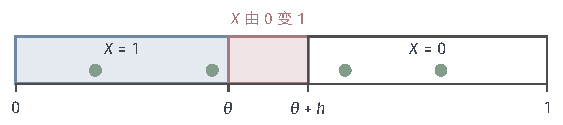
\includegraphics[width=96mm]{figures/07-probability/08-sampling-and-integration/tikz/pgrad-bernoulli-threshold/figure.pdf}
  \caption{用$X=\mathbf{1}_{\{U\leq\theta\}}$生成$\operatorname{Bern}(\theta)$。横轴是$U$的取值；蓝色区间上$X=1$。参数由$\theta=0.4$增至$\theta+h=0.55$时，只有红色区间内的$U$使$X$由$0$变为$1$，其概率为$h$。绿点是四个固定均匀数$0.37,0.80,0.15,0.62$，都不在红色区间内，它们生成的样本对参数的路径导数都是零。}
  \label{fig:pgrad-bernoulli-threshold}
\end{BookInlineFigure}

连续分布配上不连续的函数也会出同样的问题。取$f(x)=\mathbf{1}_{\{x>0\}}$，$X=\theta+\varepsilon$，则
\[
  J(\theta)=\mathbb{P}(\varepsilon>-\theta)=\Phi(\theta),\qquad J'(\theta)=\varphi(\theta)>0 .
\]对每个$\varepsilon\neq-\theta$，$f(\theta+\varepsilon)$在$\theta$附近是常数，路径导数为零。图~\ref{fig:pgrad-step-path}(a)中，四个固定噪声对应的平均$\frac{1}{4}\sum_{i}\mathbf{1}_{\{\theta+\varepsilon_{i}>0\}}$是一条阶梯，它逐段水平，导数只在台阶处“集中”。普通链式法则在这里不能直接沿用。

\begin{BookInlineFigure}
  \centering
  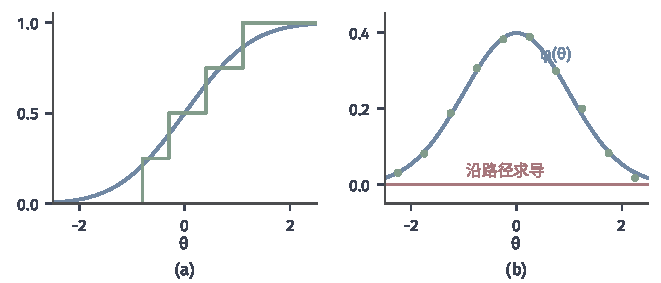
\includegraphics[width=112mm]{figures/07-probability/08-sampling-and-integration/matplotlib/pgrad-step-path/figure.pdf}
  \caption{$f(x)=\mathbf{1}_{\{x>0\}}$，$X=\theta+\varepsilon$。(a)蓝线为$J(\theta)=\Phi(\theta)$，绿色阶梯为四个固定噪声$\varepsilon=0.3,-1.1,0.8,-0.4$给出的样本平均，逐段水平。(b)蓝线为$J'(\theta)=\varphi(\theta)$，红线为路径导数的平均$0$，绿点为下一节得分函数估计在各$\theta$处的平均（每点$20000$个固定种子样本）。}
  \label{fig:pgrad-step-path}
\end{BookInlineFigure}

处理这类问题有三条出路。第一条是不对函数求导，改为对概率权重求导，这就是下一节的得分函数估计，图~\ref{fig:pgrad-step-path}(b)的绿点显示它在这个例子里给出正确的导数。第二条是把跳跃的贡献单独算出来：上例中$\frac{\mathrm{d}}{\mathrm{d}\theta}\mathbb{P}(\varepsilon>-\theta)$等于边界$\varepsilon=-\theta$处的密度，这一项可以解析地加回去。第三条是用光滑函数近似跳跃，再对近似求路径导数；这样得到的是近似问题的梯度，与原梯度的差需要另外控制。无论哪一条，都要先承认路径导数在这里不是原梯度的无偏估计。

不连续不等于不可用。若$f$是Lipschitz函数，例如$f(x)=\lvert x\rvert$，则由三角不等式
\[
  \bigl\lvert f(\theta+\varepsilon)-f(\theta'+\varepsilon)\bigr\rvert\leq\lvert\theta-\theta'\rvert,
\]
式~\eqref{eq:pgrad-lipschitz}以$M\equiv1$成立；不可微点$\theta+\varepsilon=0$只对一个$\varepsilon$出现，概率为零。于是路径导数$\operatorname{sign}(X)$的期望就是$J'(\theta)$。区分的标准不是“处处可微”，而是函数值随参数的变化能否被一个可积的Lipschitz常数控制。


\section{得分函数估计}
\label{sec:pgrad-score}

上一节最后的两个例子里，样本沿生成路径的变化是跳跃式的，路径导数看不到期望的变化。还有一些情形根本没有方便的生成映射，例如样本由Markov链产生。这时可以换一个角度：不跟踪样本点怎样移动，而看各位置的概率权重怎样变化。参数改变时，有的位置质量增加，有的减少；把函数值按这种增减加权求和，就是期望的变化率。第~\ref{chap:information-geometry}章的得分函数正好记录了每个位置上质量的相对变化率。

本节先处理密度可以完整计算的情形，再处理只知道密度到一个随参数变化的常数因子的情形。

\subsection{已归一化密度}
\label{sec:pgrad-score-normalized}

设$P_{\bm{\theta}}$相对固定的参考测度$\nu$有密度$p_{\bm{\theta}}$，支撑$S=\{x:p_{\bm{\theta}}(x)>0\}$不随$\bm{\theta}$改变。在$S$上，得分函数是
\[
  \bm{s}_{\bm{\theta}}(x)=\nabla_{\bm{\theta}}\ln p_{\bm{\theta}}(x)=\frac{\nabla_{\bm{\theta}}p_{\bm{\theta}}(x)}{p_{\bm{\theta}}(x)} .
\]
把期望写成参考测度上的积分
\[
  J(\bm{\theta})=\int_{S}f_{\bm{\theta}}\,p_{\bm{\theta}}\,\mathrm{d}\nu,
\]
在定理~\ref{thm:pgrad-exchange}中取$\mu$为$\nu$在$S$上的限制，以乘积$f_{\bm{\theta}}p_{\bm{\theta}}$作$g$。乘积的导数是
\[
  \nabla_{\bm{\theta}}(f_{\bm{\theta}}p_{\bm{\theta}})=p_{\bm{\theta}}\nabla_{\bm{\theta}}f_{\bm{\theta}}+f_{\bm{\theta}}\nabla_{\bm{\theta}}p_{\bm{\theta}}=p_{\bm{\theta}}\bigl(\nabla_{\bm{\theta}}f_{\bm{\theta}}+f_{\bm{\theta}}\bm{s}_{\bm{\theta}}\bigr),
\]
括号外的$p_{\bm{\theta}}$正好把对$\nu$的积分变回对$P_{\bm{\theta}}$的期望。

\begin{theorem}[得分函数梯度]
\label{thm:pgrad-score}
设$U$是以$\bm{\theta}_{0}$为中心的开球，所有$P_{\bm{\theta}}$（$\bm{\theta}\in U$）相对$\nu$的密度有共同支撑$S$，并且：
\begin{enumerate}
  \item 对$\nu$几乎所有$x\in S$，$p_{\bm{\theta}}(x)$与$f_{\bm{\theta}}(x)$作为$\bm{\theta}$的函数在$\bm{\theta}_{0}$处可微；
  \item 乘积$f_{\bm{\theta}}(x)p_{\bm{\theta}}(x)$作为$g(\bm{\theta},x)$，在$S$上满足定理~\ref{thm:pgrad-exchange}的条件1与条件3（取$\mu=\nu$）；
  \item $\mathbb{E}_{\bm{\theta}_{0}}\lVert\nabla_{\bm{\theta}}f_{\bm{\theta}_{0}}(X)\rVert_{2}<\infty$，且$\mathbb{E}_{\bm{\theta}_{0}}\bigl[\lvert f_{\bm{\theta}_{0}}(X)\rvert\,\lVert\bm{s}_{\bm{\theta}_{0}}(X)\rVert_{2}\bigr]<\infty$。
\end{enumerate}
则$J$在$\bm{\theta}_{0}$处可微，并且
\begin{equation}
  \nabla J(\bm{\theta}_{0})=\mathbb{E}_{\bm{\theta}_{0}}\bigl[\nabla_{\bm{\theta}}f_{\bm{\theta}_{0}}(X)+f_{\bm{\theta}_{0}}(X)\,\bm{s}_{\bm{\theta}_{0}}(X)\bigr].
  \label{eq:pgrad-score}
\end{equation}
\end{theorem}

\begin{proof}
由条件1，$g(\cdot,x)$在$\bm{\theta}_{0}$处对几乎所有$x\in S$可微，梯度是上面算出的乘积导数。结合条件2，定理~\ref{thm:pgrad-exchange}给出
\[
  \nabla J(\bm{\theta}_{0})=\int_{S}p_{\bm{\theta}_{0}}\bigl(\nabla_{\bm{\theta}}f_{\bm{\theta}_{0}}+f_{\bm{\theta}_{0}}\bm{s}_{\bm{\theta}_{0}}\bigr)\,\mathrm{d}\nu .
\]
由条件3，括号内两项分别对$P_{\bm{\theta}_{0}}$可积，积分可以拆开，各自写成期望，即得式~\eqref{eq:pgrad-score}。
\end{proof}

条件3不能由条件2推出：条件2只控制两项之和，和可积不等于每一项分别可积，而估计时两项是分开计算的。取独立样本$X_{1},\dots,X_{n}\sim P_{\bm{\theta}}$，
\begin{equation}
  \hat{\bm{g}}_{n}^{\mathrm{sf}}=\frac{1}{n}\sum_{i=1}^{n}\bigl[\nabla_{\bm{\theta}}f_{\bm{\theta}}(X_{i})+f_{\bm{\theta}}(X_{i})\,\bm{s}_{\bm{\theta}}(X_{i})\bigr]
  \label{eq:pgrad-score-estimator}
\end{equation}
称为\term{得分函数估计}（score function estimator），也称似然比方法。

\paragraph{不需要对样本位置求导}

式~\eqref{eq:pgrad-score}里出现的是$f_{\bm{\theta}}$对参数的导数和$f_{\bm{\theta}}$本身的值，从来没有$f_{\bm{\theta}}$对$x$的导数。函数可以不连续，样本空间可以是离散的，只要能在样本处求函数值、能算得分。这正是重参数化失败的地方。

对上一节的阶梯函数$f(x)=\mathbf{1}_{\{x>0\}}$与$X\sim\mathcal{N}(\theta,1)$，得分是$s(x)=x-\theta$，单样本估计为$\mathbf{1}_{\{X>0\}}(X-\theta)$。写$X=\theta+\varepsilon$，它的期望是
\[
  \mathbb{E}\bigl[\varepsilon\,\mathbf{1}_{\{\varepsilon>-\theta\}}\bigr]=\int_{-\theta}^{\infty}t\,\varphi(t)\,\mathrm{d}t=\varphi(-\theta)=\varphi(\theta),
\]
这里用到$\varphi'(t)=-t\varphi(t)$。结果正是$J'(\theta)$，图~\ref{fig:pgrad-step-path}(b)的绿点就是这个估计的样本平均。交换条件也成立：在$\lvert\theta'-\theta\rvert<1$上，
\[
  \bigl\lvert f(x)\,\partial_{\theta'}p_{\theta'}(x)\bigr\rvert\leq(\lvert x-\theta\rvert+1)\,\varphi\bigl(\max\{\lvert x-\theta\rvert-1,0\}\bigr),
\]
右边对$x$可积。

图~\ref{fig:pgrad-score-weights}从两个角度看这个估计。左图是单样本的值：$x<0$的样本贡献为零，$x>0$的样本贡献$x$，样本越靠右贡献越大。右图是$f\,\partial_{\theta}p_{\theta}$：参数增大时右半边质量增加、左半边减少，但$f$只在右半边为$1$，所以只有右半边的增量被计入，它的面积是$\varphi(0)\approx0.3989$。

\begin{BookInlineFigure}
  \centering
  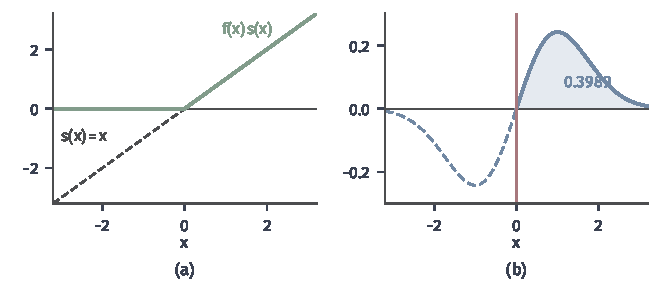
\includegraphics[width=112mm]{figures/07-probability/08-sampling-and-integration/matplotlib/pgrad-score-weights/figure.pdf}
  \caption{$X\sim\mathcal{N}(\theta,1)$在$\theta=0$处，$f(x)=\mathbf{1}_{\{x>0\}}$。(a)灰色虚线为得分$s(x)=x$，绿线为单样本估计的取值$f(x)s(x)$。(b)蓝线为$\partial_{\theta}p_{\theta}=p\,s$；红线$x=0$左侧$f=0$，这部分（虚线）不计入；右侧浅蓝面积为$\varphi(0)\approx0.3989$，等于$J'(0)$。}
  \label{fig:pgrad-score-weights}
\end{BookInlineFigure}

离散分布同样适用。$X\sim\operatorname{Bern}(\theta)$时，以计数测度为参考，$p_{\theta}(1)=\theta$，$p_{\theta}(0)=1-\theta$，得分为
\[
  s(1)=\frac{1}{\theta},\qquad s(0)=-\frac{1}{1-\theta},
\]
于是
\[
  \mathbb{E}[f(X)s(X)]=\theta\cdot\frac{f(1)}{\theta}-(1-\theta)\cdot\frac{f(0)}{1-\theta}=f(1)-f(0),
\]
正是图~\ref{fig:pgrad-bernoulli-threshold}中路径导数漏掉的那一项。

\paragraph{与重参数化在同一组样本上比较}

回到$X\sim\mathcal{N}(\mu,\sigma^{2})$、$f(x)=x^{2}$。由第~\ref{chap:information-geometry}章，两个得分分量是
\[
  s_{\mu}(x)=\frac{x-\mu}{\sigma^{2}}=\frac{\varepsilon}{\sigma},\qquad s_{\sigma}(x)=\frac{(x-\mu)^{2}-\sigma^{2}}{\sigma^{3}}=\frac{\varepsilon^{2}-1}{\sigma},
\]
其中$\varepsilon=(x-\mu)/\sigma$。用上一节同样的四个样本（$\mu=1$，$\sigma=0.5$），函数值是$f=1.3225,\ 0.2025,\ 1.9600,\ 0.6400$。$\mu$分量的单样本估计$f s_{\mu}$及其平均为
\[
  0.7935,\ -0.4455,\ 3.1360,\ -0.5120,\qquad\hat{g}_{\mu}=0.743,
\]
$\sigma$分量$f s_{\sigma}$为
\[
  -2.4069,\ 0.0851,\ -1.4112,\ -1.0752,\qquad\hat{g}_{\sigma}=-1.202 .
\]
真值是$(2,1)$，重参数化在同样的噪声上给出$(1.900,0.325)$。两种估计都无偏，但得分函数估计在这组样本上偏得更远，这不是偶然：第~\ref{sec:pgrad-variance}节会算出，在这个例子里得分函数估计的方差大得多。得分估计只利用“哪里的质量变多了”，不利用函数在样本附近怎样变化，丢掉了光滑性提供的信息。

\paragraph{支撑随参数移动}

定理~\ref{thm:pgrad-score}要求共同支撑。设$X\sim\operatorname{Unif}(0,\theta)$，$f(x)=x$，则$J(\theta)=\theta/2$，$J'(\theta)=\frac{1}{2}$。在支撑$(0,\theta)$内，$p_{\theta}(x)=1/\theta$，得分是常数$-1/\theta$。直接套用式~\eqref{eq:pgrad-score}，
\[
  \mathbb{E}_{\theta}[f(X)s_{\theta}(X)]=-\frac{1}{\theta}\mathbb{E}_{\theta}[X]=-\frac{1}{2},
\]
连符号都错了。

正确的计算要对积分上限求导。由含参积分的求导法则，
\[
  \frac{\mathrm{d}}{\mathrm{d}\theta}\int_{0}^{\theta}\frac{x}{\theta}\,\mathrm{d}x
  =\underbrace{\theta\cdot\frac{1}{\theta}}_{\text{边界}}+\int_{0}^{\theta}x\cdot\Bigl(-\frac{1}{\theta^{2}}\Bigr)\mathrm{d}x
  =1-\frac{1}{2}=\frac{1}{2}.
\]
第二项正是得分公式算出的$-\frac{1}{2}$，第一项$f(\theta)p_{\theta}(\theta^{-})=1$是新进入支撑的那一小段带来的贡献，得分只定义在旧支撑上，看不到它。第~\ref{chap:information-geometry}章用同一个均匀族说明了得分的期望在这里不为零，本例则显示加权以后漏掉的边界项可以比被计入的部分还大。

图~\ref{fig:pgrad-uniform-boundary}取$\theta=1$、$h=0.25$画出了两部分。旧支撑内$f p$从蓝线降到黄线，减少的面积是$0.1$；新增的一段$(1,1.25]$贡献$0.225$。净变化$0.125$等于$J(1.25)-J(1)$。除以$h$后两部分分别是$-0.4$与$0.9$，$h\to0$时趋于$-\frac{1}{2}$与$1$。

\begin{BookInlineFigure}
  \centering
  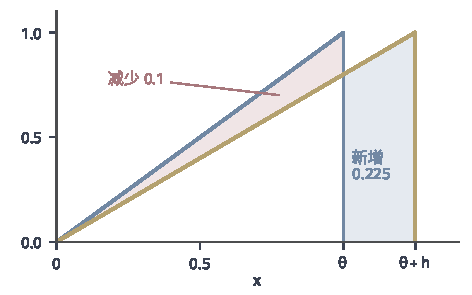
\includegraphics[width=80mm]{figures/07-probability/08-sampling-and-integration/matplotlib/pgrad-uniform-boundary/figure.pdf}
  \caption{$X\sim\operatorname{Unif}(0,\theta)$，$f(x)=x$。蓝线为$\theta=1$时的$f p_{\theta}$，黄线为$\theta+h=1.25$时的$f p_{\theta+h}$。浅红区域是旧支撑内减少的部分（面积$0.1$），得分公式只看到这一部分；浅蓝区域是新进入支撑的部分（面积$0.225$），得分公式漏掉了它。}
  \label{fig:pgrad-uniform-boundary}
\end{BookInlineFigure}

这个例子用重参数化反而没有困难：$X=\theta U$，$U\sim\operatorname{Unif}(0,1)$，路径导数$\frac{\mathrm{d}}{\mathrm{d}\theta}(\theta U)=U$，期望正是$\frac{1}{2}$。支撑的移动被样本点的移动自然地带了进去。两种方法的适用范围互补：重参数化怕函数沿路径跳跃，得分函数怕支撑随参数移动。

\subsection{未知归一化常数}
\label{sec:pgrad-score-unnormalized}

许多分布只能写到一个常数因子，例如未归一化密度取$\exp(-V_{\bm{\theta}}(x))$的形式，其中能量函数$V_{\bm{\theta}}$可以计算，而
\[
  Z_{\bm{\theta}}=\int\widetilde{p}_{\bm{\theta}}\,\mathrm{d}\nu
\]
在高维时无法直接求出。第~\ref{chap:sample-generation}章的Metropolis--Hastings采样正是为这种分布设计的：它只用到$\widetilde{p}_{\bm{\theta}}$的比值。现在要对归一化后的密度$p_{\bm{\theta}}$（即$\widetilde{p}_{\bm{\theta}}$除以$Z_{\bm{\theta}}$）下的期望求梯度，而$Z_{\bm{\theta}}$本身也随参数改变。

困难在于得分
\[
  \nabla_{\bm{\theta}}\ln p_{\bm{\theta}}=\nabla_{\bm{\theta}}\ln\widetilde{p}_{\bm{\theta}}-\nabla_{\bm{\theta}}\ln Z_{\bm{\theta}}
\]
含有$Z_{\bm{\theta}}$的导数。下面要说明，这个导数也可以写成目标分布下的期望，从而由目标样本计算。整个推导在同一个参考测度$\nu$与共同支撑$S=\{x:\widetilde{p}_{\bm{\theta}}(x)>0\}$上进行，并要求在以所论参数为中心的某个开球$U$内，每个$\bm{\theta}$都有$0<Z_{\bm{\theta}}<\infty$。需要两项交换条件：
\begin{enumerate}
  \item 归一化积分可以在积分号下求导：$\widetilde{p}_{\bm{\theta}}$在$S$上满足定理~\ref{thm:pgrad-exchange}的条件（$\mu=\nu$），于是$Z_{\bm{\theta}}$可微，梯度等于$\nabla_{\bm{\theta}}\widetilde{p}_{\bm{\theta}}$在$S$上的积分；
  \item 加权积分可以在积分号下求导：$f_{\bm{\theta}}\widetilde{p}_{\bm{\theta}}$也满足这些条件，于是加权积分
  \[
    N(\bm{\theta})=\int_{S}f_{\bm{\theta}}\widetilde{p}_{\bm{\theta}}\,\mathrm{d}\nu
  \]
  可微，梯度可在积分号下计算。
\end{enumerate}
两者缺一不可：$J=N/Z$，分子分母各自的导数都要能写成积分。

\subsubsection{得分的中心化}
\label{sec:pgrad-centering}

记未归一化密度的对数导数为
\[
  \bm{a}_{\bm{\theta}}(x)=\nabla_{\bm{\theta}}\ln\widetilde{p}_{\bm{\theta}}(x)=\frac{\nabla_{\bm{\theta}}\widetilde{p}_{\bm{\theta}}(x)}{\widetilde{p}_{\bm{\theta}}(x)},\qquad x\in S .
\]
它只用到$\widetilde{p}_{\bm{\theta}}$，可以在每个样本处计算。它和得分差多少？

\begin{lemma}[归一化常数的对数导数]
\label{lem:pgrad-logz}
在上述交换条件1下，$\bm{a}_{\bm{\theta}}(X)$在$P_{\bm{\theta}}$下可积，并且
\begin{equation}
  \nabla_{\bm{\theta}}\ln Z_{\bm{\theta}}=\mathbb{E}_{\bm{\theta}}[\bm{a}_{\bm{\theta}}(X)],
  \label{eq:pgrad-logz}
\end{equation}
从而得分是中心化的对数导数：
\begin{equation}
  \bm{s}_{\bm{\theta}}(x)=\bm{a}_{\bm{\theta}}(x)-\mathbb{E}_{\bm{\theta}}[\bm{a}_{\bm{\theta}}(X)].
  \label{eq:pgrad-centered-score}
\end{equation}
\end{lemma}

\begin{proof}
定理~\ref{thm:pgrad-exchange}的结论包含$\nabla_{\bm{\theta}}\widetilde{p}_{\bm{\theta}}$对$\nu$可积。由$\bm{a}_{\bm{\theta}}$的定义，在$S$上
\[
  \nabla_{\bm{\theta}}\widetilde{p}_{\bm{\theta}}=\widetilde{p}_{\bm{\theta}}\bm{a}_{\bm{\theta}}=Z_{\bm{\theta}}\,p_{\bm{\theta}}\bm{a}_{\bm{\theta}},
\]
所以
\[
  \mathbb{E}_{\bm{\theta}}\lVert\bm{a}_{\bm{\theta}}\rVert_{2}=\frac{1}{Z_{\bm{\theta}}}\int_{S}\lVert\nabla_{\bm{\theta}}\widetilde{p}_{\bm{\theta}}\rVert_{2}\,\mathrm{d}\nu<\infty .
\]
同一个关系与交换条件1给出
\[
  \nabla Z_{\bm{\theta}}=\int_{S}\widetilde{p}_{\bm{\theta}}\bm{a}_{\bm{\theta}}\,\mathrm{d}\nu=Z_{\bm{\theta}}\,\mathbb{E}_{\bm{\theta}}[\bm{a}_{\bm{\theta}}].
\]
因为$0<Z_{\bm{\theta}}<\infty$，两边除以$Z_{\bm{\theta}}$即得式~\eqref{eq:pgrad-logz}。最后，$\ln p_{\bm{\theta}}$与$\ln\widetilde{p}_{\bm{\theta}}$只差$\ln Z_{\bm{\theta}}$，对参数求梯度得到式~\eqref{eq:pgrad-centered-score}。
\end{proof}

这个结果的含义可以用质量的比喻说清楚。$\bm{a}_{\bm{\theta}}$记录的是未归一化质量在各位置的相对增长率，它完全可以处处为正：所有位置的质量都在增加。但概率的总量固定为$1$，归一化会把整体的增长除掉，只留下各位置相对于平均增长的差别。平均增长率按目标分布加权，就是$\mathbb{E}_{\bm{\theta}}[\bm{a}_{\bm{\theta}}]$，它等于$\ln Z_{\bm{\theta}}$的变化率。式~\eqref{eq:pgrad-centered-score}因此说：得分是相对增长率减去它的平均。中心化后的量期望为零，与第~\ref{chap:information-geometry}章得分期望为零的结论一致。

以三点分布为例。在$\{0,1,2\}$上取未归一化质量
\[
  \widetilde{p}_{\theta}(x)=h(x)\mathrm{e}^{\theta x},\qquad h=(1,2,1).
\]
此时
\[
  a_{\theta}(x)=x,\qquad Z_{\theta}=1+2\mathrm{e}^{\theta}+\mathrm{e}^{2\theta}=(1+\mathrm{e}^{\theta})^{2}.
\]
归一化后$p_{\theta}$是二项分布$\operatorname{Bin}(2,q)$，其中$q=\mathrm{e}^{\theta}/(1+\mathrm{e}^{\theta})$。直接求导得到
\[
  \frac{\mathrm{d}}{\mathrm{d}\theta}\ln Z_{\theta}=\frac{2\mathrm{e}^{\theta}}{1+\mathrm{e}^{\theta}}=2q,
\]
正是$\mathbb{E}_{\theta}[X]$，与式~\eqref{eq:pgrad-logz}一致。在$\theta=0$处，分布是$(\frac{1}{4},\frac{1}{2},\frac{1}{4})$，$a$的期望为$1$，得分是$s_{0}(x)=x-1$。

图~\ref{fig:pgrad-unnormalized}画出了这个过程。$\theta$由$0$增至$0.5$时，未归一化的三根柱子没有一根变矮；归一化以后，$x=0$处的概率从$0.25$降到约$0.14$，$x=2$处从$0.25$升到约$0.39$。$a(x)=x$全非负，减去平均$1$后才得到有正有负的得分。指数族是这个例子的一般形式：$\bm{a}_{\bm{\theta}}=\bm{T}(x)$，式~\eqref{eq:pgrad-centered-score}就是第~\ref{chap:information-geometry}章的$\bm{T}-\mathbb{E}_{\bm{\theta}}[\bm{T}]$。

\begin{BookInlineFigure}
  \centering
  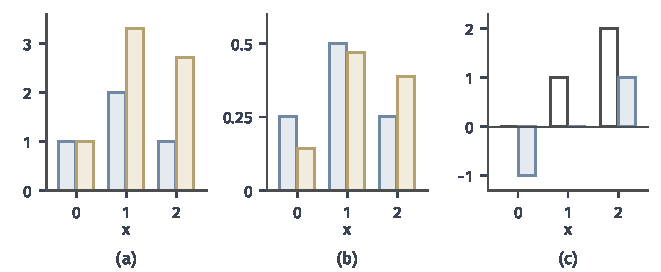
\includegraphics[width=112mm]{figures/07-probability/08-sampling-and-integration/matplotlib/pgrad-unnormalized/figure.pdf}
  \caption{$\{0,1,2\}$上的$\widetilde{p}_{\theta}(x)=h(x)\mathrm{e}^{\theta x}$，$h=(1,2,1)$。(a)未归一化质量，蓝色为$\theta=0$（总量$Z=4$），黄色为$\theta=0.5$（总量约$7.02$）；(b)归一化后的概率，质量从$x=0$移向$x=2$；(c)空心柱为$a(x)=x$，蓝色柱为$\theta=0$处的得分$s(x)=x-1$。}
  \label{fig:pgrad-unnormalized}
\end{BookInlineFigure}

\subsubsection{协方差形式}
\label{sec:pgrad-covariance}

有了中心化的得分，可以把式~\eqref{eq:pgrad-score}改写成不含$Z_{\bm{\theta}}$的形式。对标量函数$f$与向量函数$\bm{a}$，记
\[
  \operatorname{Cov}_{\bm{\theta}}(f,\bm{a})=\mathbb{E}_{\bm{\theta}}[f\bm{a}]-\mathbb{E}_{\bm{\theta}}[f]\,\mathbb{E}_{\bm{\theta}}[\bm{a}]\in\mathbb{R}^{k},
\]
它的第$j$个分量是$f$与$a_{j}$的协方差。这个定义只用到$f$、$\bm{a}$与$f\bm{a}$的可积性，不要求二阶矩。

\begin{theorem}[协方差形式的梯度]
\label{thm:pgrad-covariance}
在交换条件1与条件2下，若$f_{\bm{\theta}}$、$\nabla_{\bm{\theta}}f_{\bm{\theta}}$与$f_{\bm{\theta}}\bm{a}_{\bm{\theta}}$在$P_{\bm{\theta}}$下可积，则
\begin{equation}
  \nabla J(\bm{\theta})=\mathbb{E}_{\bm{\theta}}\bigl[\nabla_{\bm{\theta}}f_{\bm{\theta}}(X)\bigr]+\operatorname{Cov}_{\bm{\theta}}\bigl(f_{\bm{\theta}}(X),\bm{a}_{\bm{\theta}}(X)\bigr).
  \label{eq:pgrad-covariance}
\end{equation}
\end{theorem}

\begin{proof}
$J$是交换条件2中的加权积分$N$与$Z_{\bm{\theta}}$之比。由交换条件2，
\[
  \nabla N=\int_{S}\bigl(\nabla_{\bm{\theta}}f_{\bm{\theta}}+f_{\bm{\theta}}\bm{a}_{\bm{\theta}}\bigr)\widetilde{p}_{\bm{\theta}}\,\mathrm{d}\nu=Z_{\bm{\theta}}\,\mathbb{E}_{\bm{\theta}}\bigl[\nabla_{\bm{\theta}}f_{\bm{\theta}}+f_{\bm{\theta}}\bm{a}_{\bm{\theta}}\bigr],
\]
其中拆成两个期望用到了所设的可积性。由交换条件1与引理~\ref{lem:pgrad-logz}的证明，$\nabla Z_{\bm{\theta}}$等于$Z_{\bm{\theta}}\mathbb{E}_{\bm{\theta}}[\bm{a}_{\bm{\theta}}]$。商的求导法则给出
\[
  \nabla J=\frac{\nabla N}{Z_{\bm{\theta}}}-\frac{N}{Z_{\bm{\theta}}}\cdot\frac{\nabla Z_{\bm{\theta}}}{Z_{\bm{\theta}}}
  =\mathbb{E}_{\bm{\theta}}\bigl[\nabla_{\bm{\theta}}f_{\bm{\theta}}+f_{\bm{\theta}}\bm{a}_{\bm{\theta}}\bigr]-\mathbb{E}_{\bm{\theta}}[f_{\bm{\theta}}]\,\mathbb{E}_{\bm{\theta}}[\bm{a}_{\bm{\theta}}],
\]
整理即得式~\eqref{eq:pgrad-covariance}。
\end{proof}

逐个分量看，第$j$个分量的第二项是$\operatorname{Cov}_{\bm{\theta}}(f,a_{j})$。沿第$j$个参数方向，未归一化质量在$x$处按相对速率$a_{j}(x)$增长。若增长得快的地方恰好是$f$大的地方，协方差为正，期望上升；若两者无关，协方差为零，质量的增长只是整体放大，归一化后什么也没有改变。给$a_{j}$加上任何常数（各处等速增长）都不改变协方差。$\ln Z_{\bm{\theta}}$的导数正是以这种方式计入的：协方差中减去的$\mathbb{E}[f]\mathbb{E}[a_{j}]$就是那一项，而计算它只需要目标样本，不需要知道$Z_{\bm{\theta}}$。

在三点分布的例子中取$f(x)=x^{2}$，与参数无关。在$\theta=0$处，
\[
  \mathbb{E}_{0}[f]=\tfrac{0+2+4}{4}=1.5,\quad\mathbb{E}_{0}[a]=1,\quad\mathbb{E}_{0}[fa]=\mathbb{E}_{0}[X^{3}]=\tfrac{0+2+8}{4}=2.5,
\]
于是$J'(0)=\operatorname{Cov}_{0}(X^{2},X)=2.5-1.5=1$。用闭式核对：$X\sim\operatorname{Bin}(2,q)$时$J=\mathbb{E}[X^{2}]=2q+2q^{2}$，而$\mathrm{d}q/\mathrm{d}\theta=q(1-q)$，所以
\[
  J'(\theta)=(2+4q)\,q(1-q),
\]
在$q=\frac{1}{2}$处等于$4\cdot\frac{1}{4}=1$，两种算法一致。

\subsubsection{样本估计}
\label{sec:pgrad-cov-sample}

式~\eqref{eq:pgrad-covariance}中的期望与协方差都要用目标样本估计。设$X_{1},\dots,X_{n}$（$n\geq2$）独立同分布于$P_{\bm{\theta}}$，记$F_{i}=f_{\bm{\theta}}(X_{i})$，$\bm{A}_{i}=\bm{a}_{\bm{\theta}}(X_{i})$，$\bar{F}$与$\bar{\bm{A}}$为样本平均。以样本平均作中心的协方差估计取分母$n-1$：
\begin{equation}
  \hat{\bm{C}}_{n}=\frac{1}{n-1}\sum_{i=1}^{n}(F_{i}-\bar{F})(\bm{A}_{i}-\bar{\bm{A}}).
  \label{eq:pgrad-cov-estimator}
\end{equation}
梯度的估计是$\frac{1}{n}\sum_{i}\nabla_{\bm{\theta}}f_{\bm{\theta}}(X_{i})+\hat{\bm{C}}_{n}$。

为什么是$n-1$？展开乘积，
\[
  \sum_{i=1}^{n}(F_{i}-\bar{F})(\bm{A}_{i}-\bar{\bm{A}})=\sum_{i=1}^{n}F_{i}\bm{A}_{i}-n\bar{F}\bar{\bm{A}} .
\]
第一项的期望是$n\,\mathbb{E}[f\bm{a}]$。第二项里
\[
  \bar{F}\bar{\bm{A}}=\frac{1}{n^{2}}\sum_{i=1}^{n}\sum_{j=1}^{n}F_{i}\bm{A}_{j},
\]
其中$n$个$i=j$的项期望为$\mathbb{E}[f\bm{a}]$，其余$n(n-1)$项由独立性期望为$\mathbb{E}[f]\mathbb{E}[\bm{a}]$，所以
\[
  \mathbb{E}\bigl[n\bar{F}\bar{\bm{A}}\bigr]=\mathbb{E}[f\bm{a}]+(n-1)\,\mathbb{E}[f]\,\mathbb{E}[\bm{a}].
\]
两式相减，
\[
  \mathbb{E}\Bigl[\sum_{i=1}^{n}(F_{i}-\bar{F})(\bm{A}_{i}-\bar{\bm{A}})\Bigr]=(n-1)\operatorname{Cov}_{\bm{\theta}}(f,\bm{a}).
\]
用样本平均作中心时，每个样本都参与了它自己的中心，这使乘积系统地偏小，损失恰好是一个样本的份额。除以$n-1$得到无偏估计；除以$n$则期望为$\frac{n-1}{n}\operatorname{Cov}_{\bm{\theta}}(f,\bm{a})$，小样本时偏差明显。推导只用到独立同分布和$f$、$\bm{a}$、$f\bm{a}$的可积性。

用三点分布在$\theta=0$处手算一次。由逆变换，累积概率的分点是$0.25$与$0.75$，均匀数$u=0.37,0.80,0.15,0.62$给出
\[
  X=1,\ 2,\ 0,\ 1,\qquad F=1,\ 4,\ 0,\ 1,\qquad A=1,\ 2,\ 0,\ 1 .
\]
样本平均为$\bar{F}=1.5$、$\bar{A}=1$，中心化后的乘积依次是
\[
  (-0.5)\cdot0,\quad2.5\cdot1,\quad(-1.5)\cdot(-1),\quad(-0.5)\cdot0,
\]
和为$4$。除以$n-1=3$得$\hat{C}_{4}=1.333$，除以$n=4$得$1$。真值是$1$；这一组样本恰好让有偏的版本更接近真值，但平均而言它偏小$25\%$。图~\ref{fig:pgrad-cov-bias}用大量重复显示了两种分母的平均行为。

\begin{BookInlineFigure}
  \centering
  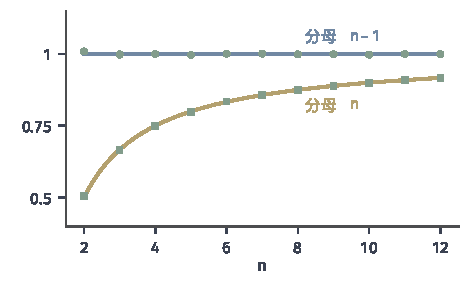
\includegraphics[width=80mm]{figures/07-probability/08-sampling-and-integration/matplotlib/pgrad-cov-bias/figure.pdf}
  \caption{三点分布$p_{0}=(\frac{1}{4},\frac{1}{2},\frac{1}{4})$上$\operatorname{Cov}(X^{2},X)=1$的两种样本估计。蓝线与绿色圆点：分母$n-1$，期望恒为$1$；黄线与绿色方块：分母$n$，期望$(n-1)/n$。线为精确期望，点为每个$n$重复$40000$次（固定种子）的平均。}
  \label{fig:pgrad-cov-bias}
\end{BookInlineFigure}

这个无偏保证依赖独立同分布。未归一化目标的样本通常来自MCMC，链上的样本相关，而且从一般初值出发时各时刻的分布还不是$P_{\bm{\theta}}$。这时推导中“$i\neq j$的项期望为$\mathbb{E}[f]\mathbb{E}[\bm{a}]$”不再成立，$n-1$分母不再修正什么，有限样本偏差由链的初值与相关性决定，要按第~\ref{sec:pgrad-approx}节与第~\ref{chap:monte-carlo-integration-error}章检查。若改用自归一化重要性采样的加权样本，加权协方差是两个随机量之比，有限样本下一般有偏，要按第~\ref{chap:variance-reduction}章对比值估计的分析检查。无偏只是一阶的性质，估计的二阶矩是否有限、波动有多大，是下一节的问题。

\section{梯度估计的方差控制}
\label{sec:pgrad-variance}

前三节得到了同一个梯度的几种表示。以$X\sim\mathcal{N}(\theta,1)$、$f(x)=x^{2}$为例，路径导数$2X$与得分估计$X^{2}(X-\theta)$的期望都是$2\theta$，它们是同一个向量期望的不同计算公式。第~\ref{chap:variance-reduction}章的观点在这里完全适用：期望相同的计算公式之间可以比较方差，也可以用控制变量和条件期望改造公式，只要改造不改变期望。

\paragraph{比较的对象}

梯度估计是$\mathbb{R}^{k}$值的，单样本$\bm{G}$的波动由协方差矩阵$\bm{\Sigma}_{\bm{G}}$描述。比较两个估计时，可以逐分量比较方差$(\bm{\Sigma}_{\bm{G}})_{j,j}$，也可以沿指定方向$\bm{u}$比较
\[
  \operatorname{Var}\bigl(\langle\bm{u},\bm{G}\rangle\bigr)=\bm{u}^{\top}\bm{\Sigma}_{\bm{G}}\bm{u},
\]
或比较式~\eqref{eq:pgrad-direct-mse}中的迹。不同分量的精度可以相差很大，第~\ref{sec:pgrad-reparam}节的高斯例子里，$\mu$分量与$\sigma$分量的单样本方差分别是$1$和$6$。这些比较都以$\mathbb{E}\lVert\bm{G}\rVert_{2}^{2}<\infty$为前提，要对每个用到的分量分别核对。

先把高斯例子的两个方差算出来。重参数化的单样本$2X$方差为$4$。得分估计是$X^{2}\varepsilon$，其中$\varepsilon=X-\theta$。求它的二阶矩要展开$(\theta+\varepsilon)^{4}\varepsilon^{2}$，所用的标准正态矩是
\[
  \mathbb{E}[\varepsilon^{2}]=1,\qquad\mathbb{E}[\varepsilon^{4}]=3,\qquad\mathbb{E}[\varepsilon^{6}]=15,
\]
奇数阶矩为零。只保留偶数次项，得到
\[
  \mathbb{E}\bigl[(\theta+\varepsilon)^{4}\varepsilon^{2}\bigr]=\theta^{4}+6\theta^{2}\cdot3+15=\theta^{4}+18\theta^{2}+15 .
\]
减去均值的平方$4\theta^{2}$，方差为$\theta^{4}+14\theta^{2}+15$。在$\theta=1$处是$30$，约为重参数化的$7.5$倍：要达到同样的精度，得分估计需要约$7.5$倍的样本。

\paragraph{得分作为控制变量}

得分估计的方差大，一个原因可以直接看出。由第~\ref{chap:information-geometry}章，正则族的得分期望为零。于是对任意常数$b$，
\[
  \mathbb{E}\bigl[(f(X)-b)\,s(X)\bigr]=\mathbb{E}[f(X)s(X)]-b\,\mathbb{E}[s(X)]=\mathbb{E}[f(X)s(X)],
\]
期望不变。项$b\,s(X)$是纯粹的噪声：它的平均为零，却随样本上下波动。在高斯例子里$f=X^{2}$总是正的，$f s$的波动有相当一部分来自$f$的平均水平乘上$s$的符号；减去一个接近$f$平均水平的$b$，就把这部分去掉了。这个常数$b$称为\term{基线}（baseline）。

这正是第~\ref{chap:variance-reduction}章的控制变量：辅助函数$h=s_{j}$的期望已知为零，系数为$b$。各分量可以用不同的基线$b_{j}$。若$\mathbb{E}[f^{2}s_{j}^{2}]<\infty$且$0<\mathbb{E}[s_{j}^{2}]<\infty$，第$j$个分量的方差是
\[
  V_{j}(b_{j})=\mathbb{E}\bigl[(f-b_{j})^{2}s_{j}^{2}\bigr]-\bigl(\mathbb{E}[f s_{j}]\bigr)^{2},
\]
它是$b_{j}$的二次函数。对$b_{j}$求导并令其为零，$-2\mathbb{E}[(f-b_{j})s_{j}^{2}]=0$，得到最优基线
\begin{equation}
  b_{j}^{*}=\frac{\mathbb{E}\bigl[f(X)\,s_{j}(X)^{2}\bigr]}{\mathbb{E}\bigl[s_{j}(X)^{2}\bigr]}.
  \label{eq:pgrad-optimal-baseline}
\end{equation}
它是按$s_{j}^{2}$加权的$f$的平均：得分大的样本对估计影响大，基线应当贴近这些样本上的函数值。由于$\mathbb{E}[s_{j}]=0$，它与控制变量的最优系数$\operatorname{Cov}(fs_{j},s_{j})/\operatorname{Var}(s_{j})$一致。

在高斯例子中，同样只保留偶数次项，
\[
  \mathbb{E}[f s^{2}]=\mathbb{E}\bigl[(\theta+\varepsilon)^{2}\varepsilon^{2}\bigr]=\theta^{2}+3,\qquad\mathbb{E}[s^{2}]=1,
\]
所以$b^{*}=\theta^{2}+3$。在$\theta=1$处，前面算出的$\mathbb{E}[f^{2}s^{2}]$等于$34$，方差作为$b$的函数是
\[
  V(b)=34-8b+b^{2}-4=b^{2}-8b+30 .
\]
三个基线的结果是
\[
  V(0)=30,\qquad V(J(1))=V(2)=18,\qquad V(b^{*})=V(4)=14 .
\]
用$J(\theta)=\mathbb{E}[f]$作基线是常见的简便选择，这里它把方差从$30$降到$18$；最优基线降到$14$。图~\ref{fig:pgrad-baseline-var}画出了这条抛物线。即使用最优基线，得分估计仍不如重参数化的$4$：常数基线只能去掉与$s$成比例的那部分噪声。

\begin{BookInlineFigure}
  \centering
  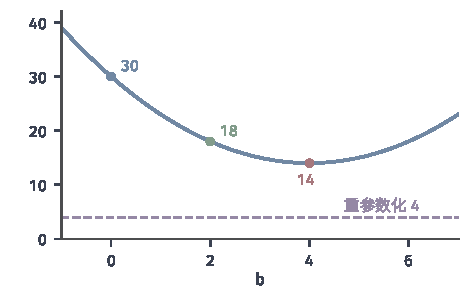
\includegraphics[width=80mm]{figures/07-probability/08-sampling-and-integration/matplotlib/pgrad-baseline-var/figure.pdf}
  \caption{$X\sim\mathcal{N}(1,1)$，$f(x)=x^{2}$。单样本估计$(f(X)-b)(X-1)$的方差$V(b)=b^{2}-8b+30$（蓝线）。蓝点为无基线$b=0$，绿点为$b=J(1)=2$，红点为最优基线$b^{*}=4$；紫色虚线为重参数化估计$2X$的方差$4$。}
  \label{fig:pgrad-baseline-var}
\end{BookInlineFigure}

\paragraph{基线所用的数据}

最优基线含有未知的期望，实际中要用样本估计。这时必须注意：$\mathbb{E}[b\,s(X)]=0$的推导要求$b$是常数，或者至少与$X$独立。若$b$由与当前样本独立的数据算出（例如先前单独抽取的一批试运行样本），则在给定这批数据的条件下$b$是常数，估计条件无偏，因而无偏。若$b$用到了当前样本本身，就要重新检查。

最自然的错误是用全部样本的平均$\bar{F}=\frac{1}{n}\sum_{j}f(X_{j})$作基线。对第$i$项，
\[
  \mathbb{E}\bigl[\bar{F}s(X_{i})\bigr]=\frac{1}{n}\mathbb{E}\bigl[f(X_{i})s(X_{i})\bigr]+\frac{1}{n}\sum_{j\neq i}\mathbb{E}[f(X_{j})]\,\mathbb{E}[s(X_{i})]=\frac{1}{n}J'(\theta),
\]
因为$\bar{F}$里含有$f(X_{i})$，它与$s(X_{i})$相关。于是
\[
  \mathbb{E}\bigl[(f(X_{i})-\bar{F})\,s(X_{i})\bigr]=\Bigl(1-\frac{1}{n}\Bigr)J'(\theta),
\]
估计系统地偏小。这和第~\ref{sec:pgrad-cov-sample}节样本协方差的偏差是同一个来源。

修正的办法是让每个样本的基线不含它自己：用其余$n-1$个样本的平均
\[
  b_{i}=\bar{F}_{-i}=\frac{1}{n-1}\sum_{j\neq i}f(X_{j}),
\]
称为\term{留一基线}（leave-one-out baseline）。$b_{i}$与$X_{i}$独立，所以$\mathbb{E}[(f(X_{i})-b_{i})s(X_{i})]=J'(\theta)$，估计无偏。由$\bar{F}_{-i}=(n\bar{F}-f(X_{i}))/(n-1)$，直接算出
\[
  f(X_{i})-\bar{F}_{-i}=\frac{n}{n-1}\bigl(f(X_{i})-\bar{F}\bigr),
\]
所以留一基线的估计恰好是全平均基线估计乘以$\frac{n}{n-1}$，与样本协方差的$n-1$分母是同一个修正。

下面用固定噪声手算。$\theta=1$，$\varepsilon=0.3,-1.1,0.8,-0.4$，样本$X=1.3,\,-0.1,\,1.8,\,0.6$，函数值与得分为
\[
  f=1.69,\ 0.01,\ 3.24,\ 0.36,\qquad s=0.3,\ -1.1,\ 0.8,\ -0.4 .
\]
不用基线时，$f s=0.507,\ -0.011,\ 2.592,\ -0.144$，平均为$0.736$。全平均为$\bar{F}=1.325$，四个留一基线是
\[
  b_{i}=1.2033,\ 1.7633,\ 0.6867,\ 1.6467,
\]
对应的$(f-b_{i})s=0.1460,\ 1.9287,\ 2.0427,\ 0.5147$，平均为$1.158$。用全平均作基线得到$0.8685$，正好是$1.158\times\frac{3}{4}$。真值是$2$。四个样本太少，三者都偏离真值，但只有前两种在平均意义下是无偏的。图~\ref{fig:pgrad-loo-baseline}用大量重复验证了全平均基线的偏差因子$\frac{n-1}{n}$。

\begin{BookInlineFigure}
  \centering
  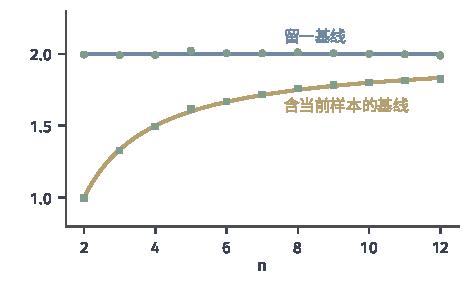
\includegraphics[width=80mm]{figures/07-probability/08-sampling-and-integration/matplotlib/pgrad-loo-baseline/figure.pdf}
  \caption{$X\sim\mathcal{N}(1,1)$，$f(x)=x^{2}$，真值$J'(1)=2$。蓝线与绿色圆点：留一基线估计的期望（恒为$2$）；黄线与绿色方块：以含当前样本的全平均作基线的估计，期望为$2(n-1)/n$。线为精确值，点为每个$n$重复$40000$次（固定种子）的平均。}
  \label{fig:pgrad-loo-baseline}
\end{BookInlineFigure}

教训是：依赖当前样本的修正不能默认无偏。留一基线之所以无偏，是因为每一项的基线与该项的得分独立；任意用当前样本拟合出来的修正项都要像上面这样逐项核对期望。

\paragraph{条件期望}

第~\ref{chap:variance-reduction}章的另一种方法是把能解析算出的随机性先积掉。设$X=(X_{1},X_{2})$，$X_{1}\sim\mathcal{N}(\theta,1)$与$X_{2}\sim\mathcal{N}(0,1)$独立，$f(x)=x_{1}^{2}+x_{2}^{2}$。参数只在$X_{1}$的分布里，得分是$s=X_{1}-\theta$，单样本得分估计为$(X_{1}^{2}+X_{2}^{2})(X_{1}-\theta)$。其中$X_{2}^{2}$与参数无关，却乘在$s$上增加波动。给定$X_{1}$对$X_{2}$取条件期望，$\mathbb{E}[X_{2}^{2}]=1$，得到改造后的估计
\[
  \mathbb{E}\bigl[(X_{1}^{2}+X_{2}^{2})s\mid X_{1}\bigr]=(X_{1}^{2}+1)(X_{1}-\theta).
\]

期望不变。记原估计为$G$，由全方差公式，方差减少的量是
\[
  \mathbb{E}\bigl[\operatorname{Var}(G\mid X_{1})\bigr]=\mathbb{E}[s^{2}]\operatorname{Var}(X_{2}^{2})=1\cdot2=2 .
\]
在$\theta=1$处可以直接核对。记$f_{1}=X_{1}^{2}$，前面已经算出$f_{1}^{2}s^{2}$与$f_{1}s^{2}$的期望分别是$34$与$4$；又$X_{2}^{2}$与$X_{2}^{4}$的期望分别是$1$与$3$。展开平方后逐项取期望，两个估计的二阶矩分别是
\[
  34+2\cdot4\cdot1+3\cdot1=45,\qquad34+2\cdot4+1=43,
\]
减去$J'(1)^{2}=4$后方差为$41$与$39$。条件化与基线可以叠加使用：在$(X_{1}^{2}+1)s$上再减去基线，就回到了一维问题的抛物线。

\paragraph{两种表示哪个更好}

在高斯二次函数的例子里，重参数化全面占优。从图~\ref{fig:pgrad-variance-compare}(a)可以看到，在$\theta\in[-2,2]$上它的方差恒为$4$，而得分估计即使配上最优基线也在$6$以上，并随$\lvert\theta\rvert$增长。但这不是普遍规律。路径导数用到$f$对$x$的导数，$f$变化剧烈时这个导数会放大波动；得分估计只用到$f$的值。

取$f(x)=\sin(\omega x)$，$X\sim\mathcal{N}(\theta,1)$。路径导数是$\omega\cos(\omega X)$，幅度随$\omega$增大；得分估计是$\sin(\omega X)(X-\theta)$，$\lvert\sin\rvert\leq1$限制了它。计算方差要用到两个高斯积分：
\[
  \mathbb{E}[\cos(cX)]=\mathrm{e}^{-c^{2}/2}\cos(c\theta),\qquad\mathbb{E}\bigl[\varepsilon^{2}\mathrm{e}^{\mathrm{i}c\varepsilon}\bigr]=(1-c^{2})\mathrm{e}^{-c^{2}/2},
\]
后者是标准正态特征函数$\mathrm{e}^{-c^{2}/2}$的二阶导数取负号。再用倍角公式把$\cos^{2}(\omega X)$与$\sin^{2}(\omega X)$写成$\cos(2\omega X)$的线性函数，在$\theta=0$处两者的方差为
\begin{align}
  \operatorname{Var}_{\mathrm{rep}}&=\frac{\omega^{2}}{2}\bigl(1+\mathrm{e}^{-2\omega^{2}}\bigr)-\omega^{2}\mathrm{e}^{-\omega^{2}},\label{eq:pgrad-sin-rep}\\
  \operatorname{Var}_{\mathrm{sf}}&=\frac{1}{2}\bigl(1-(1-4\omega^{2})\mathrm{e}^{-2\omega^{2}}\bigr)-\omega^{2}\mathrm{e}^{-\omega^{2}}.\label{eq:pgrad-sin-sf}
\end{align}

两式中减去的$\omega^{2}\mathrm{e}^{-\omega^{2}}$是$J'(0)^{2}$。$\omega\to\infty$时式~\eqref{eq:pgrad-sin-rep}像$\omega^{2}/2$那样增长，式~\eqref{eq:pgrad-sin-sf}趋于$\frac{1}{2}$。图~\ref{fig:pgrad-variance-compare}(b)显示两条曲线在$\omega\approx1.12$处相交，此后得分估计更好。

\begin{BookInlineFigure}
  \centering
  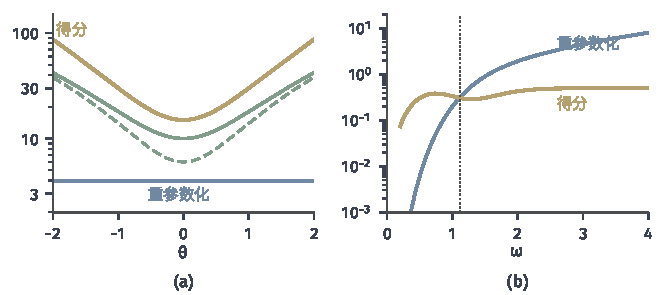
\includegraphics[width=112mm]{figures/07-probability/08-sampling-and-integration/matplotlib/pgrad-variance-compare/figure.pdf}
  \caption{$X\sim\mathcal{N}(\theta,1)$时单样本梯度估计的方差（对数纵轴）。(a)$f(x)=x^{2}$：蓝线为重参数化（恒为$4$），黄线为得分估计$\theta^{4}+14\theta^{2}+15$，绿实线为以$J(\theta)$为基线的得分估计$8\theta^{2}+10$，绿虚线为最优基线下的$8\theta^{2}+6$。(b)$f(x)=\sin(\omega x)$，$\theta=0$：蓝线为式~\eqref{eq:pgrad-sin-rep}，黄线为式~\eqref{eq:pgrad-sin-sf}，点线标出交点$\omega\approx1.12$。}
  \label{fig:pgrad-variance-compare}
\end{BookInlineFigure}

所以选择表示时不能预设哪一种更好。可用性由前几节的条件决定：函数沿路径是否受Lipschitz控制，得分能否计算，支撑是否随参数移动。在都可用的情形下，比较的是同一梯度任务下的方差与单样本成本；把这一比较放进整体预算，是下一章的内容。

\section{近似采样下的梯度}
\label{sec:pgrad-approx}

前面的无偏结论都假设样本精确服从$P_{\bm{\theta}}$。实际上，样本常常来自近似的生成器，或来自运行了有限步的Markov链。梯度公式本身是对的，用的样本却不对，结果算的是什么？

\paragraph{三个量}

设梯度公式$\bm{G}=\bm{\phi}_{\bm{\theta}}(X)$在目标下正确，即它在$X\sim P_{\bm{\theta}}$时的期望等于$\nabla J(\bm{\theta})$，而实际样本服从另一个分布$\widetilde{P}_{\bm{\theta}}$。要区分三个量：目标期望的梯度$\nabla J(\bm{\theta})$；公式在实际抽样规律下的均值
\[
  \bar{\bm{g}}(\bm{\theta})=\mathbb{E}_{\widetilde{P}_{\bm{\theta}}}[\bm{\phi}_{\bm{\theta}}(X)];
\]
以及$n$个样本平均$\hat{\bm{g}}_{n}$的有限样本波动。估计误差相应地分成两部分，
\begin{equation}
  \hat{\bm{g}}_{n}-\nabla J(\bm{\theta})=\underbrace{\bigl(\bar{\bm{g}}(\bm{\theta})-\nabla J(\bm{\theta})\bigr)}_{\text{采样偏差}}+\underbrace{\bigl(\hat{\bm{g}}_{n}-\bar{\bm{g}}(\bm{\theta})\bigr)}_{\text{有限样本波动}}.
  \label{eq:pgrad-error-split}
\end{equation}
这和第~\ref{chap:monte-carlo-integration-error}章对积分误差的分解完全相同，因为梯度估计本来就是一个积分估计。

第一部分与样本数无关，增加同一近似方法的样本数不能消除它。若$\bm{\phi}_{\bm{\theta}}$的分量有界，它可以用$\widetilde{P}_{\bm{\theta}}$与$P_{\bm{\theta}}$的总变差距离控制：对取值于$[m_{j},M_{j}]$的分量，偏差的绝对值不超过$(M_{j}-m_{j})\,d_{\mathrm{TV}}(\widetilde{P}_{\bm{\theta}},P_{\bm{\theta}})$。但梯度公式往往无界，例如得分估计里的$f\cdot s$，这时还需要尾部或矩的控制，分布在总变差下接近并不保证期望接近。第二部分取决于样本之间的关系：独立样本时它的方差是单样本方差除以$n$；样本是链上的连续状态时，要用第~\ref{chap:monte-carlo-integration-error}章的长期方差代替单样本方差，相关性可以使误差成倍增大。

\paragraph{一个可以算到底的链}

取目标$\mathcal{N}(\theta,1)$，$f(x)=x^{2}$，$J'(\theta)=2\theta$。用如下的链近似采样：
\[
  X^{(t+1)}=\rho X^{(t)}+(1-\rho)\theta+\sqrt{1-\rho^{2}}\,\varepsilon_{t},\qquad X^{(0)}=0,
\]
$\varepsilon_{t}$独立同分布于$\mathcal{N}(0,1)$，$0<\rho<1$。若$X^{(t)}\sim\mathcal{N}(\theta,1)$，则$X^{(t+1)}$的均值为$\rho\theta+(1-\rho)\theta=\theta$，方差为$\rho^{2}+1-\rho^{2}=1$，所以目标是这条链的不变分布。从$X^{(0)}=0$出发，均值与方差满足
\[
  m_{t+1}=\rho m_{t}+(1-\rho)\theta,\qquad v_{t+1}=\rho^{2}v_{t}+1-\rho^{2},
\]
解出第$K$步$X^{(K)}\sim\mathcal{N}(m_{K},v_{K})$，其中
\begin{equation}
  m_{K}=\theta(1-\rho^{K}),\qquad v_{K}=1-\rho^{2K}.
  \label{eq:pgrad-ar-law}
\end{equation}

把目标下正确的两个公式用在$X^{(K)}$上。重参数化公式$2X$的均值是$2m_{K}=2\theta(1-\rho^{K})$；得分公式$X^{2}(X-\theta)$的均值是
\[
  \mathbb{E}\bigl[(X^{(K)})^{3}\bigr]-\theta\,\mathbb{E}\bigl[(X^{(K)})^{2}\bigr]=m_{K}^{3}+3m_{K}v_{K}-\theta(m_{K}^{2}+v_{K}).
\]
取$\theta=1$、$\rho=0.8$、$K=5$，$\rho^{5}=0.32768$，于是$m_{5}=0.6723$，$v_{5}=0.8926$。两个公式的均值分别为
\[
  2m_{5}=1.345,\qquad m_{5}^{3}+3m_{5}v_{5}-(m_{5}^{2}+v_{5})=0.760,
\]
目标是$2$。同一组近似样本上，两个在目标下都无偏的公式偏差不同，偏差的大小取决于公式本身。

\paragraph{对有限步程序求导}

另一种做法是把整个采样程序当成生成映射，对它做重参数化。展开递推，$X^{(K)}$是$\theta$的仿射函数加上与$\theta$无关的噪声，$\partial X^{(K)}/\partial\theta=1-\rho^{K}$，路径导数为$2X^{(K)}(1-\rho^{K})$。这里每一步都合法：噪声分布固定，函数光滑，交换条件也容易验证。它的期望是程序所定义的期望
\[
  J_{K}(\theta)=\mathbb{E}\bigl[(X^{(K)})^{2}\bigr]=\theta^{2}(1-\rho^{K})^{2}+1-\rho^{2K}
\]
的导数$J_{K}'(\theta)=2\theta(1-\rho^{K})^{2}$，在上面的参数下等于$0.904$，而不是$J'(1)=2$。

也就是说，对有限步采样程序求导并交换积分，得到的是程序期望$J_{K}$的导数；它是否等于目标期望$J$的导数，是另一个需要证明的命题。本例中$J_{K}$对$\theta$的依赖还包含初值$X^{(0)}=0$不随$\theta$移动这一人为因素，所以$J_{K}'$比两个“目标公式”偏得更多。图~\ref{fig:pgrad-chain-bias}画出了三个量随步数$K$的变化，图~\ref{fig:pgrad-error-split}在$K=5$处把式~\eqref{eq:pgrad-error-split}的两部分和程序导数放在一条数轴上比较。

\begin{BookInlineFigure}
  \centering
  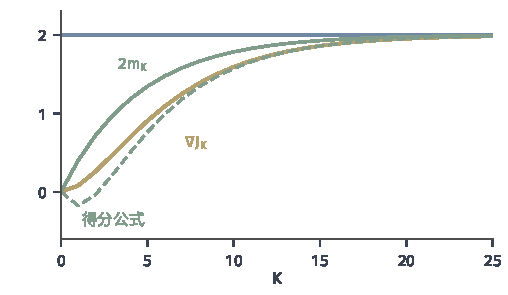
\includegraphics[width=86mm]{figures/07-probability/08-sampling-and-integration/matplotlib/pgrad-chain-bias/figure.pdf}
  \caption{目标$\mathcal{N}(1,1)$、$f(x)=x^{2}$，样本取自从$0$出发、$\rho=0.8$的链的第$K$步。蓝线为目标梯度$2$；绿实线为重参数化公式$2X$在第$K$步分布下的均值$2m_{K}$；绿虚线为得分公式$X^{2}(X-1)$在同一分布下的均值；黄线为有限步程序期望的导数$J_{K}'$。}
  \label{fig:pgrad-chain-bias}
\end{BookInlineFigure}

\begin{BookInlineFigure}
  \centering
  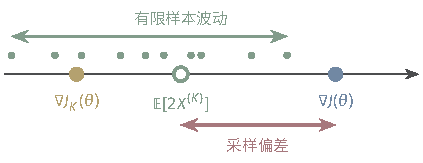
\includegraphics[width=72mm]{figures/07-probability/08-sampling-and-integration/tikz/pgrad-error-split/figure.pdf}
  \caption{图~\ref{fig:pgrad-chain-bias}中$K=5$时的误差分解。蓝点为目标梯度$\nabla J(1)=2$；绿圈为公式$2X$在实际抽样规律下的均值$1.345$，它与蓝点之差是采样偏差；上方绿点为$10$次独立重复中$n=20$个样本平均的取值（固定种子），其散布是有限样本波动；黄点为有限步程序的导数$0.904$。}
  \label{fig:pgrad-error-split}
\end{BookInlineFigure}

\paragraph{步数增加时}

本例中$K\to\infty$时三个量都趋于$2$，因为式~\eqref{eq:pgrad-ar-law}给出了闭式。一般情形下，即使$J_{K}\to J$，也推不出$J_{K}'\to J'$。例如
\[
  J_{K}(\theta)=J(\theta)+\frac{1}{K}\sin(K\theta)
\]
满足$\lvert J_{K}-J\rvert\leq1/K$，但$J_{K}'-J'=\cos(K\theta)$不趋于零。函数值的一致逼近不控制导数。要由程序导数得到目标导数，需要导数本身的收敛，例如$J_{K}'$在$\theta$的某个邻域上一致收敛，这时微积分中关于导数一致收敛的定理保证极限就是$J'$。对实际的MCMC程序，这类结论要用到链对参数的可微依赖与遍历性的定量估计，超出了本卷给定分布计算的范围。

实际计算时，比较稳妥的做法是：用前几节在目标下成立的梯度公式，把链上的样本当作计算这个期望的积分样本，然后按第~\ref{chap:monte-carlo-integration-error}章检查初值偏差、相关性与长期方差。这样，梯度的正确性来自目标下的公式，误差的分析来自积分误差的理论，两者各有依据。

\section{本章小结}
\label{sec:pgrad-summary}

章首的问题是：样本平均$\frac{1}{n}\sum_{i}X_{i}^{2}$里看不到参数，对它求导得到零，可$\mathbb{E}[X^{2}]$明明随$\theta$变化。答案是参数通过样本的来源进入了期望，求梯度时必须把它找出来并计入。本章的做法是先把参数的位置看清，再把期望写成某个固定测度上的积分，参数全部移进被积函数，然后用定理~\ref{thm:pgrad-exchange}的局部Lipschitz控制检查求导能否移进积分。逐点可微不够，图~\ref{fig:pgrad-moving-spike}的移动尖峰就是反例。

三种表示对应三种固定测度的选法，各自利用不同的计算条件，也各有失效的情形。

\begin{BookInlineTable}
  \centering
  \caption{三种梯度表示的比较。}
  \label{tab:pgrad-methods}
  \begin{tabular}{@{}llll@{}}
    \toprule
    & 直接求导 & 重参数化 & 得分函数 \\
    \midrule
    固定的测度 & 抽样分布$P$ & 噪声分布$Q$ & 参考测度$\nu$ \\
    需要计算 & $\nabla_{\bm{\theta}}f_{\bm{\theta}}$ & 生成映射及$\nabla_{x}f_{\bm{\theta}}$ & 得分或$\bm{a}_{\bm{\theta}}$ \\
    对$f$的要求 & 对参数可控 & 沿路径可控 & 可求值即可 \\
    典型失效 & 控制不可积 & 离散选择、跳跃 & 支撑随参数移动 \\
    \bottomrule
  \end{tabular}
\end{BookInlineTable}

直接求导适用于抽样分布固定的情形，梯度就是逐样本导数的平均。重参数化把分布的变化改写成样本点的移动，路径导数由链式法则的两条路组成；函数沿路径跳跃时它看不到跳跃的贡献。得分函数估计对概率权重求导，不需要$f$对$x$可微，离散变量与不连续函数都能处理；但它要求支撑不随参数移动，否则会漏掉边界项。归一化常数未知时，得分是未归一化对数导数减去它的期望，梯度化为函数值与对数导数的协方差，只需目标样本；用独立样本估计时，以样本平均为中心的协方差要除以$n-1$。

无论用哪种表示，都要分开检查两件事：梯度样本的可积性保证估计无偏和一致，二阶矩才保证误差按$n^{-1/2}$缩小。不同表示的方差可以相差很多，没有哪一种在所有问题上更好；得分估计可以借助得分期望为零加入基线，基线若用到当前样本，须像留一基线那样保证与该样本的得分独立。样本来自近似生成器或有限步链时，估计误差分成与样本数无关的采样偏差和有限样本波动；对有限步程序求导得到的是程序期望的导数，它与目标导数是否相同要另行证明。

本章只回答怎样把期望的导数变成可估计的积分，以及这个估计的偏差与波动。用这些梯度逐步更新参数，是随机优化的问题。下一章在共同的精度要求下，比较各种采样、方差控制与梯度表示的计算预算，讨论怎样为具体任务选择方法。


\chapter{计算预算与方法选择}
\label{chap:sampling-budget-method-selection}

设要计算$X\sim\operatorname{Exp}(1)$超过$4$的概率$I=\mathbb{P}(X>4)=\mathrm{e}^{-4}\approx0.0183$，要求在$95\%$的把握下相对误差不超过$10\%$，可用的计算量折合$10^{5}$次函数求值。前几章给了很多工具：可以直接平均示性函数，可以改用指数分布$\operatorname{Exp}(\lambda)$作建议分布做重要性采样，也可以先花一些计算量做试运行，再决定$\lambda$。哪一种能在预算内完成任务？“相对误差$10\%$”是不是合适的要求？试运行该花多少？什么时候可以停下来报告结果？

这些问题不是新的数学对象，而是把前四章的结论放到同一本账上。第~\ref{chap:sample-generation}章给出生成样本的各种办法，第~\ref{chap:monte-carlo-integration-error}章说明样本平均的偏差与波动怎样估计，第~\ref{chap:variance-reduction}章讨论怎样在积分不变的前提下减小方差，第~\ref{chap:expectation-gradient-estimation}章把这些方法推广到含参期望的梯度。每一章都在“其他条件不变”的前提下比较方法；实际计算时，误差要求、样本成本、预备开销和停止方式都要同时考虑。

本章按做一次计算的顺序展开。第~\ref{sec:budget-targets}节先确定要控制什么误差，第~\ref{sec:budget-costs}节统一成本的口径，第~\ref{sec:budget-allocation}节把预算分给试运行、正式计算、多条链或多组随机化，第~\ref{sec:budget-selection}节按可计算的信息选择采样、方差控制与梯度估计方法，第~\ref{sec:budget-stopping}节讨论试运行之后怎样固定方案、何时停止。全章反复使用前几章的几个例子：尾概率$\mathrm{e}^{-4}$及其重要性采样，$\mathrm{e}^{u}$在$[0,1]$上的积分$\mathrm{e}-1$及其方差控制，以$\mathcal{N}(0,1)$为不变分布的自回归链，以及双峰混合$0.3\,\mathcal{N}(-2,0.5^{2})+0.7\,\mathcal{N}(2,1)$。

\section{计算目标与精度要求}
\label{sec:budget-targets}

比较方法之前，先要说清楚算什么、算到什么程度算完。待算的量是固定的数：积分$I=\mathbb{E}_{\pi}[f]$，或者含参期望$J(\bm{\theta})$在某一点的梯度$\nabla J(\bm{\theta})\in\mathbb{R}^{d}$。随机的是计算过程，估计$\hat{I}_n$随所用随机数而变。“精度”因此是对$\hat{I}_n-I$这个随机误差的要求，而同一个误差可以用几种不同的方式来约束。不同的约束会要求很不一样的样本数，有的在目标接近零时还会失去意义。

\paragraph{三种误差口径}
最直接的要求是误差的绝对值$\lvert\hat{I}_n-I\rvert$不超过给定的$\varepsilon$。但$\hat{I}_n$是随机的，任何有限样本都可能偶然偏得很远，所以“误差不超过$\varepsilon$”只能以平均或概率的方式表达。第一种是要求\term{均方误差}（mean squared error）不超过$\varepsilon^{2}$。按第~\ref{chap:monte-carlo-integration-error}章的分解，在$\hat{I}_n$二阶矩有限时
\begin{equation}
  \mathbb{E}\bigl[(\hat{I}_n-I)^{2}\bigr]=\bigl(\mathbb{E}[\hat{I}_n]-I\bigr)^{2}+\operatorname{Var}(\hat{I}_n),
  \label{eq:budget-mse}
\end{equation}
右边第一项是偏差的平方，第二项是随机波动。均方误差把两者放在同一个单位下相加，便于在它们之间权衡。

第二种是指定概率下的误差：给定容差$\varepsilon>0$和允许的失败概率$\delta\in(0,1)$，要求
\begin{equation}
  \mathbb{P}\bigl(\lvert\hat{I}_n-I\rvert>\varepsilon\bigr)\le\delta .
  \label{eq:budget-eps-delta}
\end{equation}
它直接回答“这次计算有多大把握落在容差以内”。两种口径之间有一个总成立的桥：对误差平方用Markov不等式，
\[
  \mathbb{P}\bigl(\lvert\hat{I}_n-I\rvert>\varepsilon\bigr)\le\frac{\mathbb{E}\bigl[(\hat{I}_n-I)^{2}\bigr]}{\varepsilon^{2}} .
\]
所以只要均方误差不超过$\delta\varepsilon^{2}$，式~\eqref{eq:budget-eps-delta}就成立。这一步不需要任何分布假设，代价是保守。

对独立同分布、方差为$\sigma^{2}$的无偏样本平均，$\operatorname{Var}(\hat{I}_n)=\sigma^{2}/n$，上面的充分条件给出样本数
\begin{equation}
  n_{\mathrm{Cheb}}=\frac{\sigma^{2}}{\delta\varepsilon^{2}} .
  \label{eq:budget-n-cheb}
\end{equation}
若改用中心极限定理的正态近似，记$z_{1-\delta/2}$为标准正态的$1-\delta/2$分位数，需要的样本数约为
\begin{equation}
  n_{\mathrm{N}}\approx\frac{z_{1-\delta/2}^{2}\,\sigma^{2}}{\varepsilon^{2}} .
  \label{eq:budget-n-normal}
\end{equation}
后者只是渐近近似，覆盖保证不是有限样本下精确的；前者是有限样本下成立的上界。两者的差别完全来自对$\delta$的依赖：Chebyshev界按$1/\delta$增长，正态近似中的$z_{1-\delta/2}^{2}$只按$\ln(1/\delta)$的量级增长。

以$\mathrm{e}^{u}$在$[0,1]$上的积分$I=\mathrm{e}-1$为例，直接平均$\mathrm{e}^{U}$的单样本方差是
\[
  \sigma^{2}=\frac{\mathrm{e}^{2}-1}{2}-(\mathrm{e}-1)^{2}\approx0.2420 .
\]
取$\varepsilon=0.01$、$\delta=0.05$，由式~\eqref{eq:budget-n-cheb}与式~\eqref{eq:budget-n-normal}，
\[
  n_{\mathrm{Cheb}}=\frac{0.2420}{0.05\times10^{-4}}\approx48\,400,\qquad n_{\mathrm{N}}\approx\frac{1.96^{2}\times0.2420}{10^{-4}}\approx9\,300 .
\]
两者相差约$5.2$倍。图~\ref{fig:budget-n-requirement}(a)画出$\delta$变化时这两个样本数：$\delta$越小，Chebyshev界与正态近似的距离越大。选择哪一个，要看报告需要有限样本的保证，还是可以接受渐近近似。

\begin{BookInlineFigure}
  \centering
  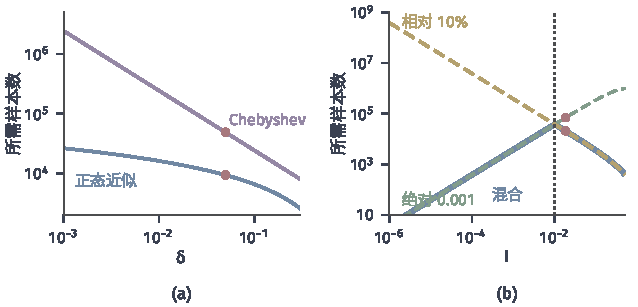
\includegraphics[width=108mm]{figures/07-probability/08-sampling-and-integration/matplotlib/budget-n-requirement/figure.pdf}
  \caption{误差口径决定所需样本数。(a)~积分$\mathrm{e}-1$、容差$\varepsilon=0.01$：紫线为Chebyshev界式~\eqref{eq:budget-n-cheb}，蓝线为正态近似式~\eqref{eq:budget-n-normal}，红点为$\delta=0.05$。(b)~尾概率$I$的直接平均在$95\%$正态近似下所需的样本数：绿色虚线为绝对容差$0.001$，黄色虚线为相对容差$10\%$，蓝色粗线为二者取较宽者的混合容差；竖直点线$I=0.01$是两种容差相等处，红点对应$I=\mathrm{e}^{-4}$。}
  \label{fig:budget-n-requirement}
\end{BookInlineFigure}

梯度的目标是向量$\nabla J(\bm{\theta})\in\mathbb{R}^{d}$，误差用欧氏范数衡量。设估计$\hat{\bm{g}}$的均值为$\bm{m}$，协方差矩阵为$\bm{\Sigma}_{\hat{g}}$，逐分量应用式~\eqref{eq:budget-mse}再相加，得到
\begin{equation}
  \mathbb{E}\bigl[\lVert\hat{\bm{g}}-\nabla J\rVert_2^{2}\bigr]=\lVert\bm{m}-\nabla J\rVert_2^{2}+\operatorname{tr}\bm{\Sigma}_{\hat{g}} .
  \label{eq:budget-vector-mse}
\end{equation}
波动部分是协方差矩阵的迹，即各分量方差之和。若只关心某个方向$\bm{v}$上的变化率，相应的误差只涉及$\bm{v}^{\top}\bm{\Sigma}_{\hat{g}}\bm{v}$，比全向量的要求宽松得多。第~\ref{sec:budget-gradient-choice}节会看到，按迹比较时各种梯度估计的优劣可能与按单个分量比较时不同。

\paragraph{相对误差与接近零的目标}
当待算量很小时，绝对容差$0.001$可能比答案本身还大，于是人们常改用\term{相对误差}（relative error）$\lvert\hat{I}_n-I\rvert/\lvert I\rvert$。对尾概率，相对要求才有意义：$I=\mathrm{e}^{-4}\approx0.0183$时，报告$0.0183\pm0.001$与报告$0.0183\pm0.0002$说明的事情差别不大，但报告$0.0183\pm0.0183$就没有说明任何事。问题出在$I$趋于零时。直接平均示性函数的单样本方差是$I(1-I)$，相对容差$\varepsilon_{\mathrm{rel}}$在正态近似下要求
\[
  n\approx\frac{z^{2}I(1-I)}{(\varepsilon_{\mathrm{rel}}I)^{2}}=\frac{z^{2}(1-I)}{\varepsilon_{\mathrm{rel}}^{2}\,I},
\]
其中$z=1.96$。它随$I\to0$按$1/I$增长；$I=0$时这个要求无法满足，因为任何非零的估计都有无穷大的相对误差。

目标恰为零或可能为零的情形很常见：一个奇函数在对称分布下的期望，参数取到最优点时的梯度，两种方案期望之差在二者一样好时的取值。这时只用相对误差会使计算无限进行下去。实用的写法是给一个\term{混合容差}（mixed tolerance）：
\begin{equation}
  \lvert\hat{I}_n-I\rvert\le\max\bigl\{\varepsilon_{\mathrm{abs}},\ \varepsilon_{\mathrm{rel}}\lvert I\rvert\bigr\} .
  \label{eq:budget-mixed-tolerance}
\end{equation}
目标较大时相对项起作用，目标接近零时绝对项兜底。对梯度，把式中的绝对值换成欧氏范数即可；在参数接近最优点时梯度本身趋于零，这时只有绝对项能给出可以达到的要求。$\varepsilon_{\mathrm{abs}}$不是随意的：它表示“比这更小的差别对使用者已无意义”的尺度，应由任务本身给出。

用尾概率走一遍。$I=\mathrm{e}^{-4}$时单样本方差$I(1-I)\approx0.01798$。绝对容差$0.001$与相对容差$10\%$在正态近似下分别要求
\[
  n_{\mathrm{abs}}\approx\frac{1.96^{2}\times0.01798}{10^{-6}}\approx69\,100,\qquad n_{\mathrm{rel}}\approx\frac{1.96^{2}\times0.9817}{0.01\times0.01832}\approx20\,600 .
\]
混合容差取二者中较宽的$\max\{0.001,0.00183\}=0.00183$，所需样本数就是$20\,600$。图~\ref{fig:budget-n-requirement}(b)把这三条曲线画成$I$的函数：相对容差的曲线在$I\to0$时向上发散，绝对容差的曲线向下，混合容差取二者的较小者，在两种容差相等的$I=0.01$处转折。

还要注意：混合容差里的$\lvert I\rvert$本身未知，实际判断只能用估计值代替。这个代替在估计值远离零时无害，在估计值接近零时会把相对项估得过小或过大，第~\ref{sec:budget-stopping}节讨论依据数据决定何时停止时还会回到这一点。

\paragraph{固定预算与固定精度}
同一个误差要求可以从两个方向提出。一是预算$C$给定，在所有可行方案中使误差最小；二是误差要求给定，使达到它的成本最小。用均方误差写，二者分别是
\begin{equation}
  \min_{\text{方案}}\ \mathrm{MSE}\quad\text{使}\ \text{成本}\le C,
  \qquad
  \min_{\text{方案}}\ \text{成本}\quad\text{使}\ \mathrm{MSE}\le\varepsilon^{2}.
  \label{eq:budget-two-problems}
\end{equation}
对无偏的独立样本平均，两个问题等价。设每个样本的成本为$c$、方差为$\sigma^{2}$，预算$C$可买$n=C/c$个样本，于是
\begin{equation}
  \mathrm{MSE}\cdot C=\frac{\sigma^{2}}{n}\cdot nc=\sigma^{2}c .
  \label{eq:budget-mse-cost-product}
\end{equation}
乘积$\sigma^{2}c$与预算无关：给定预算时误差是$\sigma^{2}c/C$，给定误差时成本是$\sigma^{2}c/\varepsilon^{2}$，哪个方案的$\sigma^{2}c$小，它在两种提法下都更好。第~\ref{sec:budget-costs}节会把$\sigma^{2}c$作为比较的基本量。

有偏差时情况不同。偏差不随样本数减小，它通常由方法的某个参数控制，例如数值离散的步长；而缩小偏差往往使每个有效样本更贵。这时固定预算与固定精度的答案都要在偏差和波动之间折中，而且固定精度的问题可能对某些参数根本无解：若偏差本身已经超过$\varepsilon$，增加样本只会把误差压到偏差为止。

下面用第~\ref{chap:monte-carlo-integration-error}章的近似链说明这种折中。目标是$\pi=\mathcal{N}(0,1)$，被积函数$f(x)=x^{2}$，$I=1$。用步长$h\in(0,1)$的链
\begin{equation}
  X^{(t+1)}=(1-h)X^{(t)}+\sqrt{2h}\,\varepsilon^{(t)},\qquad\varepsilon^{(t)}\sim\mathcal{N}(0,1)\ \text{独立},
  \label{eq:budget-ula-chain}
\end{equation}
每步成本记为$1$。这条链的不变分布不是目标：对平稳的方差$v$，由$v=(1-h)^{2}v+2h$解得$v=2/(2-h)$。于是平稳时的偏差
\[
  b(h)=v-1=\frac{h}{2-h}.
\]

再算波动。记$\rho=1-h$。平稳的高斯自回归链中，$X^{(0)}$与$X^{(k)}$是协方差为$v\rho^{k}$的联合高斯变量，由高斯四阶矩公式，
\[
  \operatorname{Cov}\bigl((X^{(0)})^{2},(X^{(k)})^{2}\bigr)=2\bigl(v\rho^{k}\bigr)^{2}=2v^{2}\rho^{2k}.
\]
代入第~\ref{chap:monte-carlo-integration-error}章的长期方差（$\gamma_{0}$加上各阶自协方差之和的两倍），对几何级数求和，得到
\[
  \sigma_{\mathrm{LR}}^{2}(h)=2v^{2}\Bigl(1+2\sum_{k\ge1}\rho^{2k}\Bigr)=\frac{2v^{2}(1+\rho^{2})}{1-\rho^{2}}=\frac{2v^{2}\bigl(1+(1-h)^{2}\bigr)}{h(2-h)} .
\]
从平稳状态启动、运行$B$步时，均方误差在$B$较大时为
\begin{equation}
  \mathrm{MSE}(h,B)\approx b(h)^{2}+\frac{\sigma_{\mathrm{LR}}^{2}(h)}{B} .
  \label{eq:budget-ula-mse}
\end{equation}
步长越小，偏差越小，但链的相关越强，波动越大。

对小$h$取主项，$b(h)\approx h/2$，$\sigma_{\mathrm{LR}}^{2}(h)\approx2/h$，于是
\[
  \mathrm{MSE}(h,B)\approx\frac{h^{2}}{4}+\frac{2}{hB}.
\]
对$h$求导并令其为零，$h/2-2/(h^{2}B)=0$，解得最优步长和最小均方误差
\begin{equation}
  h^{\ast}\approx\Bigl(\frac{4}{B}\Bigr)^{1/3},\qquad\mathrm{MSE}^{\ast}\approx\frac34\cdot4^{2/3}B^{-2/3}\approx1.89\,B^{-2/3}.
  \label{eq:budget-ula-opt}
\end{equation}
均方根误差按$B^{-1/3}$下降，比无偏样本平均的$B^{-1/2}$慢。原因是每增加预算，最优安排都要把一部分花在缩小步长上，而不是全部用于平均。

图~\ref{fig:budget-ula-tradeoff}(a)按式~\eqref{eq:budget-ula-mse}的精确表达式画出三种预算下的均方误差：左侧是波动主导，右侧贴近偏差平方$b(h)^{2}$，红点是最优步长。$B=10^{4}$时数值最优$h^{\ast}\approx0.071$，均方误差约$0.0043$，均方根误差约$0.065$；从$\mathcal{N}(0,1)$直接独立抽样时$\operatorname{Var}(X^{2})=2$，同样预算的均方根误差是$\sqrt{2/10^{4}}\approx0.014$。图~\ref{fig:budget-ula-tradeoff}(b)比较两种方法达到均方根误差$\varepsilon=0.01$所需的预算：精确采样需要$2/\varepsilon^{2}=2\times10^{4}$步，近似链即使每次都取最优步长也需要约$2.6\times10^{6}$步。

\begin{BookInlineFigure}
  \centering
  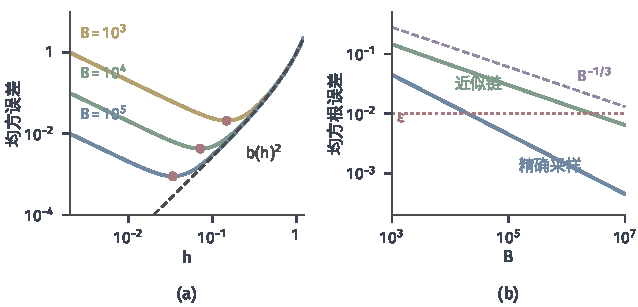
\includegraphics[width=108mm]{figures/07-probability/08-sampling-and-integration/matplotlib/budget-ula-tradeoff/figure.pdf}
  \caption{近似链~\eqref{eq:budget-ula-chain}在偏差与波动之间的折中，$f(x)=x^{2}$，目标$\mathcal{N}(0,1)$，从平稳状态启动。(a)~三种预算$B$下的均方误差随步长$h$变化，深灰虚线为偏差平方$b(h)^{2}$，红点为最优步长。(b)~均方根误差随预算变化：蓝线为独立精确抽样，绿线为每个预算下取最优步长的近似链，紫色虚线为$B^{-1/3}$参考斜率，红色点线为容差$\varepsilon=0.01$。}
  \label{fig:budget-ula-tradeoff}
\end{BookInlineFigure}

这个例子还说明，式~\eqref{eq:budget-two-problems}两种提法的结论都依赖偏差项是否存在。对无偏方法，只需比较$\sigma^{2}c$；对有偏方法，必须同时选择控制偏差的参数，固定精度的要求会把预算推到偏差允许的范围。式~\eqref{eq:budget-ula-mse}忽略了初值的影响，从非平稳状态启动时还要加上第~\ref{chap:monte-carlo-integration-error}章所说的初始偏差，它在这里按$1/(hB)$衰减，不改变$B^{-1/3}$的量级。

\section{计算成本}
\label{sec:budget-costs}

式~\eqref{eq:budget-mse-cost-product}说明，无偏方法之间比较的是“单样本方差乘单样本成本”。可是“一个样本”在不同方法里含义不同：拒绝采样的一个输出要先生成并淘汰若干候选，Markov链每步都产生一个状态但相邻状态高度相关，有的方法在抽第一个样本之前就要做一次矩阵分解或一轮试运行。要让比较公平，就要把这些开销记在同一本账上，并且明确“成本”是按什么单位计的。

\paragraph{成本的组成}
一次随机计算的开销可以分成三类。第一类是每次迭代的操作：生成基础随机数，按建议分布生成候选，计算目标密度、密度比或梯度，计算被积函数。第二类把迭代换算成输出：拒绝采样平均要做若干次迭代才输出一个样本，抽稀的链每$k$步才保存一个状态。第三类只发生一次或每条链一次：矩阵分解、试运行与建议分布的拟合、控制系数或分层方案的预估，以及链开始时为摆脱初值而舍弃的$b$步。

记一次迭代的成本为$c_{\mathrm{it}}$，一个输出样本的成本为$c_{\mathrm{out}}$，一次性开销为$C_{0}$。输出$n$个样本的总成本是
\begin{equation}
  C=C_{0}+b\,c_{\mathrm{it}}+n\,c_{\mathrm{out}} .
  \label{eq:budget-total-cost}
\end{equation}
图~\ref{fig:budget-cost-ledger}把这几项的关系画成一张账：单项操作合成一次迭代，迭代乘以候选数或抽稀间隔得到输出样本，输出样本再乘以相关性的影响得到下文的有效样本。计成本的单位可以是运行时间，也可以是某种主导操作的次数（如目标密度的计算次数）。用操作次数便于复现和推导，用时间更贴近实际，二者在向量化、缓存或并行时可能给出不同的排序，比较前要说明用的是哪一种。

\begin{BookInlineFigure}
  \centering
  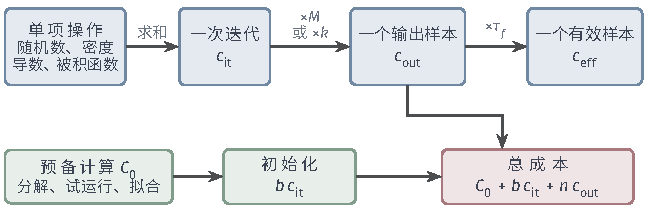
\includegraphics[width=110mm]{figures/07-probability/08-sampling-and-integration/tikz/budget-cost-ledger/figure.pdf}
  \caption{一次随机计算的成本账。上排是按单位累积的成本：单项操作合成一次迭代$c_{\mathrm{it}}$，拒绝采样乘以平均候选数$M$、抽稀乘以间隔$k$得到一个输出样本$c_{\mathrm{out}}$，相关链再乘以$\tau_{f}$得到针对被积函数$f$的一个有效样本。下排是只计一次的开销：预备计算$C_{0}$和每条链初始化舍弃的$b$步，它们与$n$个输出的成本合成总成本~\eqref{eq:budget-total-cost}。}
  \label{fig:budget-cost-ledger}
\end{BookInlineFigure}

\paragraph{工作量归一化方差}
设某个无偏方法的输出相互独立，单样本方差为$\sigma^{2}$，单样本成本为$c$，一次性开销为$C_{0}$，暂不考虑初始化。总预算$C>C_{0}$可买$n=(C-C_{0})/c$个样本（忽略取整），估计的方差为
\begin{equation}
  \operatorname{Var}(\hat{I})=\frac{\sigma^{2}c}{C-C_{0}} .
  \label{eq:budget-var-budget}
\end{equation}
称$\sigma^{2}c$为\term{工作量归一化方差}（work-normalized variance）。预算远大于$C_{0}$时，它是比较两种方法的唯一量：方法甲优于方法乙，当且仅当$\sigma_{\text{甲}}^{2}c_{\text{甲}}<\sigma_{\text{乙}}^{2}c_{\text{乙}}$。单看方差或单看成本都会误判：方差小一半而每个样本贵三倍的方法，在同样预算下反而更差。

一次性开销使比较依赖预算。设方法乙没有预备开销，方法甲有$C_{0}>0$且$\sigma_{\text{甲}}^{2}c_{\text{甲}}<\sigma_{\text{乙}}^{2}c_{\text{乙}}$。由式~\eqref{eq:budget-var-budget}，甲的方差较小当且仅当
\[
  \frac{\sigma_{\text{甲}}^{2}c_{\text{甲}}}{C-C_{0}}<\frac{\sigma_{\text{乙}}^{2}c_{\text{乙}}}{C},
\]
整理得
\begin{equation}
  C>C_{\times}=\frac{C_{0}\,\sigma_{\text{乙}}^{2}c_{\text{乙}}}{\sigma_{\text{乙}}^{2}c_{\text{乙}}-\sigma_{\text{甲}}^{2}c_{\text{甲}}} .
  \label{eq:budget-crossover}
\end{equation}
预算低于$C_{\times}$时，花在准备上的成本收不回来。

以第~\ref{chap:variance-reduction}章的尾概率为例。直接平均的$\sigma^{2}=I(1-I)\approx0.01798$，每个样本成本记为$1$；从$\operatorname{Exp}(1/4)$抽样的重要性采样单样本方差约$0.001749$，每个样本成本记为$1.5$，选定建议分布的预备开销记为$C_{0}=2000$。两者的工作量归一化方差分别为
\[
  0.01798\times1=0.01798,\qquad0.001749\times1.5\approx0.002623,
\]
大预算下重要性采样约好$6.9$倍。代入式~\eqref{eq:budget-crossover}，
\[
  C_{\times}=\frac{2000\times0.01798}{0.01798-0.002623}\approx2342 .
\]
本章开头的预算$10^{5}$远超过它，准备是值得的。

\paragraph{拒绝候选与矩阵分解}
拒绝采样的每个候选被接受的概率是$1/M$，$M$为包络常数（第~\ref{chap:sample-generation}章）。各候选独立，所以得到一个输出所需的候选数$N$服从参数$1/M$的几何分布，$\mathbb{P}(N=j)=(1-1/M)^{j-1}/M$，其均值为
\[
  \mathbb{E}[N]=\sum_{j\ge1}j\Bigl(1-\frac1M\Bigr)^{j-1}\frac1M=\frac{1/M}{(1/M)^{2}}=M .
\]
若每个候选要生成一次建议样本（成本$c_{q}$）、计算一次接受判据（成本$c_{\mathrm{acc}}$），被接受的样本还要计算一次被积函数（成本$c_{f}$），则
\begin{equation}
  c_{\mathrm{out}}=M\,(c_{q}+c_{\mathrm{acc}})+c_{f} .
  \label{eq:budget-rejection-cost}
\end{equation}
被淘汰的候选不产生输出，但其成本全额计入。$M$随维数增长时，这一项可能成为全部成本的主体。

生成$\mathcal{N}(\bm{\mu},\bm{\Sigma})$的样本时，要先把$d\times d$的协方差矩阵分解为$\bm{\Sigma}=\bm{L}\bm{L}^{\top}$，此后每个样本是$\bm{\mu}+\bm{L}\bm{Z}$。按\BookChapterRef{chap:direct-linear-solvers}{卷二第12章“线性方程的直接求解”}，Cholesky分解约需$d^{3}/3$次乘加，下三角矩阵乘向量约需$d^{2}$次。抽$n$个样本时，平均到每个样本的乘加次数约为
\[
  \frac{d^{3}/3}{n}+d^{2}=d^{2}\Bigl(1+\frac{d}{3n}\Bigr).
\]
$n$远大于$d$时分解的开销可以忽略；$n$与$d$相当或更小时（例如$d=1000$只抽$100$个样本），分解占了大部分成本，这时比较方法必须把$C_{0}$计入，而不能只看每个样本的$d^{2}$。

\paragraph{迭代、输出样本与有效样本}
Markov链每步输出一个状态，相邻状态相关，保存下来的状态数不能直接当作样本数。设链平稳，被积函数$f$的单步方差为$\gamma_{0}$，长期方差为$\sigma_{\mathrm{LR}}^{2}$，记
\begin{equation}
  \tau_{f}=\frac{\sigma_{\mathrm{LR}}^{2}}{\gamma_{0}},\qquad N_{\mathrm{eff}}=\frac{N}{\tau_{f}} .
  \label{eq:budget-tau}
\end{equation}
这里的$N_{\mathrm{eff}}$就是第~\ref{chap:monte-carlo-integration-error}章的有效样本量：$N$步相关平均的渐近方差$\sigma_{\mathrm{LR}}^{2}/N$等于$N_{\mathrm{eff}}$个独立样本的方差$\gamma_{0}/N_{\mathrm{eff}}$。于是忽略初始化时，针对$f$的一个有效样本的成本是
\begin{equation}
  c_{\mathrm{eff}}=c_{\mathrm{it}}\,\tau_{f},
  \label{eq:budget-eff-cost}
\end{equation}
相关链的工作量归一化方差是
\[
  \gamma_{0}\,c_{\mathrm{eff}}=\gamma_{0}c_{\mathrm{it}}\tau_{f}=\sigma_{\mathrm{LR}}^{2}c_{\mathrm{it}} .
\]

$\tau_{f}$属于“链与被积函数”这一对，而不是只属于链。以平稳自回归链
\begin{equation}
  X^{(t+1)}=\rho X^{(t)}+\sqrt{1-\rho^{2}}\,\varepsilon^{(t)},\qquad\varepsilon^{(t)}\sim\mathcal{N}(0,1)\ \text{独立}
  \label{eq:budget-ar1}
\end{equation}
为例，目标$\mathcal{N}(0,1)$。对$f(x)=x$，$\gamma_{k}=\rho^{k}$；对$f(x)=x^{2}$，$\gamma_{k}=2\rho^{2k}$。分别对几何级数求和，得到
\[
  \tau_{x}=\frac{1+\rho}{1-\rho},\qquad\tau_{x^{2}}=\frac{1+\rho^{2}}{1-\rho^{2}} .
\]
$\rho=0.9$时$\tau_{x}=19$，$\tau_{x^{2}}\approx9.53$：同一条链的同一段记录，估计$\mathbb{E}[X^{2}]$时的有效样本数约是估计$\mathbb{E}[X]$时的两倍。图~\ref{fig:budget-ess-thinning}(a)画出每步的有效样本数$1/\tau_{f}$随$\rho$的变化。

\begin{BookInlineFigure}
  \centering
  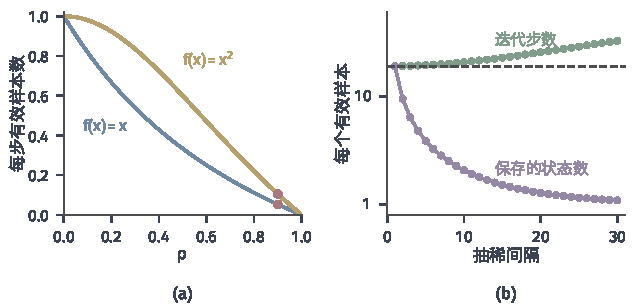
\includegraphics[width=108mm]{figures/07-probability/08-sampling-and-integration/matplotlib/budget-ess-thinning/figure.pdf}
  \caption{平稳自回归链（目标$\mathcal{N}(0,1)$）的有效样本。(a)~每步迭代提供的有效样本数$1/\tau_{f}$：蓝线$f(x)=x$，黄线$f(x)=x^{2}$，红点为$\rho=0.9$。(b)~$\rho=0.9$、$f(x)=x$时每隔$k$步保存一个状态：绿线为每个有效样本所需的迭代步数，紫线为所需保存的状态数，深灰虚线为不抽稀时的$19$步。}
  \label{fig:budget-ess-thinning}
\end{BookInlineFigure}

保存时常做\term{抽稀}（thinning）：每$k$步只保存一个状态。抽稀后的序列仍是自回归链，系数为$\rho^{k}$，长度为$N/k$。对$f(x)=x$，每个有效样本需要保存$(1+\rho^{k})/(1-\rho^{k})$个状态，相应的迭代步数是
\[
  k\,\frac{1+\rho^{k}}{1-\rho^{k}} .
\]
$\rho=0.9$、$k=10$时，前者约$2.07$，后者约$20.7$，比不抽稀的$19$步还多。图~\ref{fig:budget-ess-thinning}(b)显示了这一点：抽稀减少存储，不减少计算，对这个例子还略微损失精度。只有被积函数本身很贵，例如每次求值的成本$c_{f}$远大于一步转移的成本时，抽稀才能节省计算，因为这时每个保存状态的成本是$k\,c_{\mathrm{it}}+c_{f}$，适当的$k$可以减少昂贵的求值次数。

链的初始化另有成本。每条链舍弃前$b$步，花费$b\,c_{\mathrm{it}}$，这一项不随保存的样本数摊薄，启动的链越多，总的初始化成本越高。第~\ref{sec:budget-allocation}节比较多次启动与单链延长时会用到这一点。

\paragraph{三种采样方式的成本比较}
把上面的账用到第~\ref{chap:sample-generation}章的双峰混合
\[
  \pi=0.3\,\mathcal{N}(-2,0.5^{2})+0.7\,\mathcal{N}(2,1)
\]
上，被积函数取$f(x)=x$。这时
\[
  I=0.3\times(-2)+0.7\times2=0.8,\qquad\operatorname{Var}_{\pi}(f)=0.3\times4.25+0.7\times5-0.8^{2}=4.135 .
\]

作为教学约定，取成本单位：一个均匀数记$1$，一个标准高斯数记$2$，计算一次混合密度记$4$（两个指数），计算一次单个高斯包络的密度记$2$，计算一次$f$记$1$。三种方式的单样本成本如下。
\begin{itemize}
  \item 分步生成：先用一个均匀数选成分，再生成一个高斯数，最后算$f$，$c_{\mathrm{out}}=1+2+1=4$，样本独立，$\tau_{f}=1$。
  \item 拒绝采样：在网格上选使$M$最小的高斯包络，得到$\mathcal{N}(0.25,2.2^{2})$，$M\approx2.29$，接受率约$0.44$。每个候选要一个高斯数、一次包络密度、一次目标密度和一个均匀数，共$9$，由式~\eqref{eq:budget-rejection-cost}，$c_{\mathrm{out}}\approx9\times2.29+1\approx21.7$。
  \item 随机游走Metropolis：每步一个高斯数、一次目标密度、一个均匀数和一次$f$，$c_{\mathrm{it}}=8$。$\tau_{f}$由$10^{6}$步链的分块均值估计，步长$s=1,2.5,4$时分别约为$66$、$8.5$、$6.5$。
\end{itemize}

由式~\eqref{eq:budget-eff-cost}，Metropolis每个有效样本的成本分别约为$527$、$68$、$52$。图~\ref{fig:budget-sampler-costs}(b)把五个数放在对数坐标上：对这个一维目标，分步生成比最好的链便宜十几倍，拒绝采样介于其间。若只按“保存的状态数”比较，Metropolis每步成本$8$只是拒绝采样的约三分之一，结论正好相反。图~\ref{fig:budget-sampler-costs}(a)给出原因：步长$s=1$时，状态要在两个峰之间往返，自相关衰减很慢；步长较大时接受率降低，但跨峰更容易，$\tau_{f}$反而小得多。

\begin{BookInlineFigure}
  \centering
  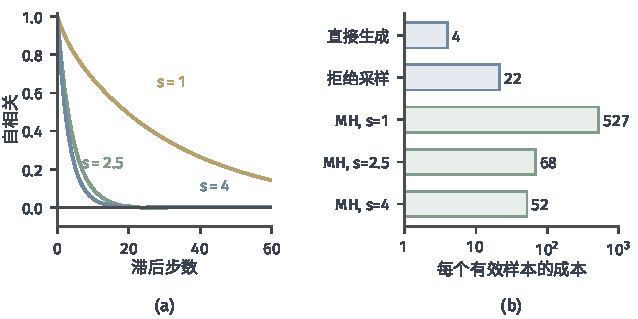
\includegraphics[width=108mm]{figures/07-probability/08-sampling-and-integration/matplotlib/budget-sampler-costs/figure.pdf}
  \caption{双峰混合$0.3\,\mathcal{N}(-2,0.5^{2})+0.7\,\mathcal{N}(2,1)$、$f(x)=x$时三种采样方式的成本（教学约定的操作计数）。(a)~随机游走Metropolis的自相关函数，三条线对应步长$s=1,2.5,4$，各由$10^{6}$步链计算。(b)~每个有效样本的成本：蓝色为独立样本，绿色为Metropolis（每步成本乘以估计的$\tau_{f}$）。}
  \label{fig:budget-sampler-costs}
\end{BookInlineFigure}

这里的$\tau_{f}$是从一段有限记录估计的，它本身有误差，而且只有在链确实走遍两个峰时才可信；第~\ref{sec:budget-stopping}节会看到有限记录可能完全没有发现某个峰。比较结论还依赖成本单位：若目标密度极贵而高斯数几乎免费，各项的比例会改变。账本的作用是让这些假设明确可查，而不是给出与假设无关的排名。

\section{预算分配}
\label{sec:budget-allocation}

有了成本账，下一个问题是同一笔预算怎样分。几乎每种改进都要求先花一部分计算去“了解问题”：重要性采样要先拟合建议分布，控制变量要先估计系数，分层要先知道各层的波动，Markov链要先跑掉初值的影响。花得太少，方案选得差；花得太多，留给正式计算的就少了。成组随机化还有另一种分法：总点数一定时，每组放多少点、重复多少组。

\paragraph{试运行与正式计算}
设总预算为$C$。先用$n_{0}$个试运行样本（每个成本$c_{0}$）确定方法的参数$\hat{\lambda}$，再用剩下的预算按$\hat{\lambda}$做正式计算，每个正式样本成本为$c$。正式计算使用与试运行独立的新随机数，所以在给定试运行结果的条件下，正式估计仍是无偏的独立样本平均（第~\ref{chap:variance-reduction}章对固定建议后的估计证明了这一点），其条件方差为$v(\hat{\lambda})c/(C-n_{0}c_{0})$，这里$v(\lambda)$是参数取$\lambda$时的单样本方差。对试运行取期望，最终估计的方差是
\begin{equation}
  \operatorname{Var}(\hat{I})=\frac{\mathbb{E}\bigl[v(\hat{\lambda})\bigr]\,c}{C-n_{0}c_{0}} .
  \label{eq:budget-pilot-var}
\end{equation}
分子随$n_{0}$增大而减小，因为参数估得更准；分母也随$n_{0}$增大而减小，因为正式计算的预算变少。

为看清两种作用怎样平衡，设$\hat{\lambda}$随$n_{0}\to\infty$收敛到$\bar{\lambda}$，$v$在$\bar{\lambda}$附近光滑，且$\hat{\lambda}-\bar{\lambda}$的均方按$1/n_{0}$缩小。

若$\bar{\lambda}$是$v$的最小点，展开到二阶，一阶项消失；若不是，$\hat{\lambda}$的偏差与波动也只在$1/n_{0}$阶贡献额外方差。两种情形都可以写成
\[
  \mathbb{E}\bigl[v(\hat{\lambda})\bigr]\approx\bar{v}+\frac{a}{n_{0}},
\]
其中$\bar{v}=v(\bar{\lambda})$，$a>0$概括参数估计误差的影响。代入式~\eqref{eq:budget-pilot-var}，要最小化
\[
  g(n_{0})=\frac{\bar{v}+a/n_{0}}{C-n_{0}c_{0}} .
\]
令$g'(n_{0})=0$，即
\[
  -\frac{a}{n_{0}^{2}}\,(C-n_{0}c_{0})+c_{0}\Bigl(\bar{v}+\frac{a}{n_{0}}\Bigr)=0,
\]
两边乘以$n_{0}^{2}$并整理，得到
\[
  c_{0}\bar{v}\,n_{0}^{2}+2ac_{0}\,n_{0}-aC=0 .
\]
取正根，并在$C$远大于$ac_{0}/\bar{v}$时保留主项，得到
\begin{equation}
  n_{0}^{\ast}\approx\sqrt{\frac{aC}{c_{0}\bar{v}}},\qquad\frac{n_{0}^{\ast}c_{0}}{C}\approx\sqrt{\frac{ac_{0}}{\bar{v}C}} .
  \label{eq:budget-pilot-opt}
\end{equation}
试运行的样本数按$\sqrt{C}$增长，占总预算的比例按$1/\sqrt{C}$缩小。预算越大，越值得把参数估准，但越不必为此花上一个固定的比例。

用本章开头的尾概率演示。试运行从覆盖尾部的$q_{0}=\operatorname{Exp}(1/2)$抽样，每个样本对积分的贡献为$c_{i}=\mathbf{1}_{\{Y_i>4\}}p(Y_i)/q_{0}(Y_i)$。第~\ref{chap:variance-reduction}章说明理想的建议分布正比于$\mathbf{1}_{\{x>4\}}\mathrm{e}^{-x}$，其均值为$5$。在指数族$\operatorname{Exp}(\lambda)$中，用贡献加权的均值去匹配$1/\lambda$：
\[
  \hat{\lambda}=\frac{\sum_{i}c_i}{\sum_{i}c_iY_i},
\]
试运行没有样本超过$4$时保留$\lambda=1/2$。$n_{0}\to\infty$时$\hat{\lambda}\to1/5$，此时单样本方差$v(0.2)\approx0.001738$，与族内最优$\lambda^{\ast}\approx0.219$处的$v^{\ast}\approx0.001730$只差$0.5\%$。试运行与正式样本的成本都记为$1.5$。

图~\ref{fig:budget-pilot-size}画出三种预算下最终的相对均方根误差$\sqrt{\operatorname{Var}(\hat{I})}/I$随$n_{0}$的变化，条件方差用精确公式计算，对试运行的期望用模拟（种子$7$）。三条曲线的谷底都很平：$C=1500$时最好的$n_{0}$约为$37$，相对均方根误差约$0.074$，比已知最优建议分布的$0.072$只差一点；$n_{0}$小到$5$时误差约$0.084$，只高出约$14\%$；$n_{0}$大到预算的$70\%$时误差约$0.131$，高出约$78\%$。作为对照，同样预算的直接平均相对误差约为$0.19$。三种预算的最优$n_{0}$随$C$右移，但远慢于$C$本身的增长，与式~\eqref{eq:budget-pilot-opt}一致。

\begin{BookInlineFigure}
  \centering
  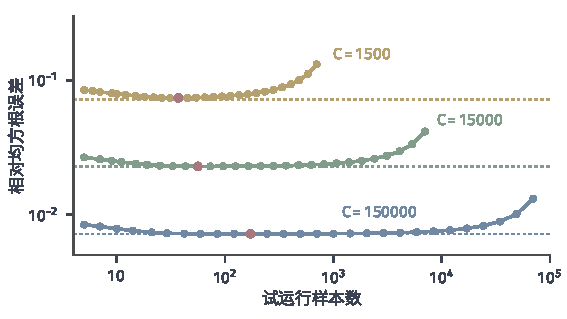
\includegraphics[width=96mm]{figures/07-probability/08-sampling-and-integration/matplotlib/budget-pilot-size/figure.pdf}
  \caption{试运行规模与最终精度。目标$I=\mathbb{P}(X>4)$，$X\sim\operatorname{Exp}(1)$；试运行从$\operatorname{Exp}(1/2)$抽取$n_{0}$个样本拟合$\lambda$，正式计算用新随机数从$\operatorname{Exp}(\hat{\lambda})$抽样，每个样本成本$1.5$。三条曲线对应总预算$C=1500$、$15000$、$150000$，点线为已知最优$\lambda^{\ast}$时的误差，红点为各曲线的最小点。}
  \label{fig:budget-pilot-size}
\end{BookInlineFigure}

这个例子的拟合问题很容易，只有一个参数，所以谷底特别平。参数多、贡献区域分散时，$a$会大得多，过小的试运行可能根本没有观察到某个贡献区域，这时式~\eqref{eq:budget-pilot-opt}所依据的“误差按$1/n_{0}$缩小”还没有开始成立。第~\ref{sec:budget-stopping}节讨论这种情形。

\paragraph{预备开销的分摊}
控制变量的系数也可以由试运行估计。用$n_{0}$个独立的试运行样本估计$\hat{\beta}$，再用新样本计算$f-\hat{\beta}(h-\mathbb{E}h)$的平均，给定$\hat{\beta}$时正式估计无偏，方差为$\operatorname{Var}\bigl(f-\hat{\beta}h\bigr)/n$，分析与式~\eqref{eq:budget-pilot-var}相同。若用同一批样本既估系数又求平均，省下了试运行，却引入$1/n$阶的有限样本偏差（第~\ref{chap:variance-reduction}章），预算较大时这一偏差相对于波动可以忽略，预算很小时则要计入。

分层采样把预备开销与分配规则联系在一起。设$K$层的概率为$p_k$，层内单样本方差为$\sigma_k^{2}$，层内每个样本的成本为$c_k$，第$k$层抽$n_k$个样本。

分层估计的方差与总成本分别是
\[
  \sum_{k=1}^{K}\frac{p_k^{2}\sigma_k^{2}}{n_k},\qquad\sum_{k=1}^{K}n_kc_k=C .
\]
由Cauchy--Schwarz不等式，
\[
  \Bigl(\sum_{k}p_k\sigma_k\sqrt{c_k}\Bigr)^{2}=\Bigl(\sum_{k}\frac{p_k\sigma_k}{\sqrt{n_k}}\cdot\sqrt{n_kc_k}\Bigr)^{2}\le\sum_{k}\frac{p_k^{2}\sigma_k^{2}}{n_k}\cdot\sum_{k}n_kc_k,
\]
等号当且仅当$\sqrt{n_kc_k}$与$p_k\sigma_k/\sqrt{n_k}$成比例。于是固定预算下的最优分配与最小方差为
\begin{equation}
  n_k\propto\frac{p_k\sigma_k}{\sqrt{c_k}},\qquad\operatorname{Var}_{\min}=\frac{1}{C}\Bigl(\sum_{k=1}^{K}p_k\sigma_k\sqrt{c_k}\Bigr)^{2} .
  \label{eq:budget-neyman-cost}
\end{equation}

式~\eqref{eq:budget-neyman-cost}要求知道各层的$\sigma_k$和$c_k$，实际只能由试运行估计，而估计的成本与估计误差都要计入。按$n_k\propto p_k$的比例分配不需要这些信息，在样本总数相同时其方差不超过直接平均；把预算从比例分配转向式~\eqref{eq:budget-neyman-cost}，只有在试运行能可靠区分各层波动时才值得。

以$\mathrm{e}^{U}$的$4$层等概率分层为例，各层成本相同，层内标准差依次约为$0.082$、$0.105$、$0.135$、$0.173$。比例分配与式~\eqref{eq:budget-neyman-cost}的最优分配按每个样本折算的方差分别为
\[
  \sum_{k}p_k\sigma_k^{2}\approx0.01653,\qquad\Bigl(\sum_{k}p_k\sigma_k\Bigr)^{2}\approx0.01536,
\]
最优分配把样本按约$0.17:0.21:0.27:0.35$分给四层，只多省约$7\%$。若为估计$\sigma_k$专门做一轮试运行，这点收益很容易被试运行的成本和$\sigma_k$的估计误差抵消；直接平均的$0.2420$到比例分层的$0.0165$才是主要的改进。

\paragraph{多次启动与单链延长}
Markov链的预算$B$（总迭代步数）可以给一条长链，也可以分给$m$条短链，每条$B/m$步，各自舍弃前$b$步。用式~\eqref{eq:budget-ar1}中$\rho=0.9$的自回归链计算，目标$\mathcal{N}(0,1)$，$f(x)=x$，$I=0$，所有链都从$x_{0}=10$启动。这条链的矩可以精确写出：
\[
  \mathbb{E}\bigl[X^{(t)}\bigr]=0.9^{t}x_{0},\qquad\operatorname{Cov}\bigl(X^{(s)},X^{(t)}\bigr)=0.9^{\lvert t-s\rvert}\bigl(1-0.81^{\min(s,t)}\bigr),
\]
于是每种分法的均方误差都可以精确计算。

图~\ref{fig:budget-chain-count}给出$B=2000$时的结果。不舍弃初值（$b=0$）时，一条链的均方误差约$0.0115$，其中偏差约$0.045$；分成$10$条链后偏差升到约$0.45$，均方误差约$0.21$。原因是每条链都带着同样的初值偏差，平均多条链不能抵消它，而每条链越短，初值那一段所占的比例越大。舍弃$b=30$步后，一条链的均方误差约$0.0096$，接近平稳时的$\sigma_{\mathrm{LR}}^{2}/B=19/2000=0.0095$；链数增多，$mb$步的初始化成本吃掉越来越多的预算，$m=50$时均方误差升到约$0.076$。对单峰、链混合良好的目标，只看均方误差，一条长链最省。

单链时舍弃多少步也可以由均方误差估算。设舍弃$b$步后保留$L=B-b$步，初值偏差在平均中留下的部分约为
\[
  \frac{x_{0}}{L}\sum_{t=b+1}^{B}\rho^{t}\approx\frac{x_{0}\rho^{b+1}}{(1-\rho)L},
\]
波动约为$\sigma_{\mathrm{LR}}^{2}/L$。$b$每增加$1$，偏差平方约乘以$\rho^{2}$，减少量约为偏差平方的$2\ln(1/\rho)$倍；波动则因$L$减少$1$而约增加$\sigma_{\mathrm{LR}}^{2}/L^{2}$。在最优的$b$处二者相等，
\[
  2\ln\frac1\rho\cdot\frac{x_{0}^{2}\rho^{2b+2}}{(1-\rho)^{2}L^{2}}=\frac{\sigma_{\mathrm{LR}}^{2}}{L^{2}},
  \qquad\text{即}\qquad
  \rho^{2b+2}=\frac{\sigma_{\mathrm{LR}}^{2}(1-\rho)^{2}}{2x_{0}^{2}\ln(1/\rho)} .
\]
代入$\rho=0.9$、$x_{0}=10$、$\sigma_{\mathrm{LR}}^{2}=19$，右边约为$0.0090$，解得$b\approx21$，与精确计算的最优值$21$一致。舍弃步数只按$\ln x_{0}$增长：初值离目标越远，舍弃越多，但远小于总预算。这个估算要求知道链向目标靠拢的速度$\rho$，一般的链只能由试运行或理论估计。

\begin{BookInlineFigure}
  \centering
  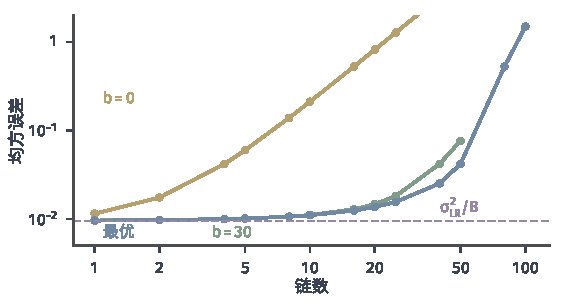
\includegraphics[width=96mm]{figures/07-probability/08-sampling-and-integration/matplotlib/budget-chain-count/figure.pdf}
  \caption{总预算$B=2000$步分给$m$条链时的精确均方误差。自回归链系数$0.9$，目标$\mathcal{N}(0,1)$，$f(x)=x$，每条链从$x_{0}=10$启动并舍弃前$b$步。黄线$b=0$，绿线$b=30$，蓝线对每个$m$取最优$b$；紫色虚线为平稳单链的$\sigma_{\mathrm{LR}}^{2}/B$。}
  \label{fig:budget-chain-count}
\end{BookInlineFigure}

多次启动的价值在别处：它是发现链没有走遍目标的少数手段之一。图~\ref{fig:budget-multistart}在双峰混合$0.3\,\mathcal{N}(-2,0.5^{2})+0.7\,\mathcal{N}(2,1)$上用步长$s=0.5$的随机游走Metropolis，从$-4,-1,1,4$四个分散的初值各跑$500$步。从$-4$与$-1$出发的两条链始终留在左峰，平均约$-2.0$；从$4$出发的一条始终在右峰，平均约$2.15$；从$1$出发的一条在第$270$步左右才跨到左峰。只看任何一条链，运行均值都会在某个错误的值附近“稳定”下来。

\begin{BookInlineFigure}
  \centering
  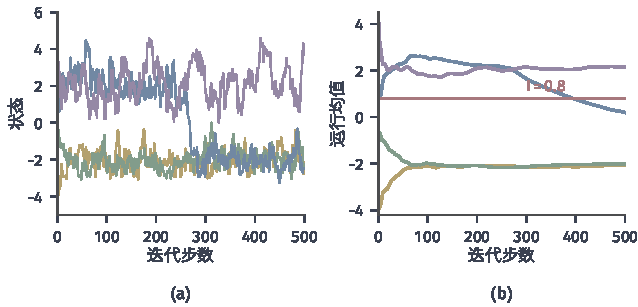
\includegraphics[width=108mm]{figures/07-probability/08-sampling-and-integration/matplotlib/budget-multistart/figure.pdf}
  \caption{双峰混合$0.3\,\mathcal{N}(-2,0.5^{2})+0.7\,\mathcal{N}(2,1)$上的随机游走Metropolis（步长$0.5$），四条链分别从$-4$（黄）、$-1$（绿）、$1$（蓝）、$4$（紫）启动，种子$0$到$3$。(a)~状态轨迹。(b)~$f(x)=x$的运行均值，红线为$I=0.8$。}
  \label{fig:budget-multistart}
\end{BookInlineFigure}

四条链之间的差异立刻暴露了问题，但把它们合起来平均并不能修正：合并均值约$-0.43$，因为四条链在两个峰上的时间比例反映的是初值的安排，而不是两个峰的概率$0.3$与$0.7$。所以多条链的分歧只能说明“当前的转移核在这个预算内不够用”，补救要回到转移核本身，例如加大步长（图~\ref{fig:budget-sampler-costs}中$s=4$的$\tau_{f}$约为$6.5$）。在预算分配上，这意味着要在单链延长带来的较小相关误差与多次启动带来的探索检查之间取舍：前者对已经走遍目标的链更经济，后者对可能多峰的目标是必要的保险。

\paragraph{成组采样的组内点数与重复数}
拉丁超立方与随机化准蒙特卡洛一次产生一组相关的点，第~\ref{chap:monte-carlo-integration-error}章说明误差要靠整组的独立重复来估计。设每组$n$个点，重复$R$组，总求值次数$N=nR$，另加点集准备的成本。两个参数的作用不同：$n$决定单组估计$Q$的精度，$R$是估计$\operatorname{Var}(Q)$时的独立观测数。

以随机移位网格$a_k=k/n$计算$\int_{0}^{1}\mathrm{e}^{u}\,\mathrm{d}u$为例。单组估计的方差有精确表达式，对大的$n$约为$(\mathrm{e}-1)^{2}/(12n^{2})$（第~\ref{chap:variance-reduction}章）。代入$n=N/R$，$R$组平均的方差为
\[
  \frac{\operatorname{Var}(Q_{n})}{R}\approx\frac{(\mathrm{e}-1)^{2}}{12n^{2}R}=\frac{(\mathrm{e}-1)^{2}R}{12N^{2}} .
\]
总点数固定时，组数越少，平均越准，因为单组方差随$n$下降得比$1/n$快。

可是只有$R$个组估计可用来估计方差，误差区间要用自由度$R-1$的$t$分位数$t_{R-1}$，形如$\bar{Q}\pm t_{R-1}s_{Q}/\sqrt{R}$。$R=2$时$t_{1}\approx12.7$，区间极宽。图~\ref{fig:budget-groups}(a)取$N=1024$，比较平均的均方根误差与区间的平均半宽：均方根误差随$R$单调增大，半宽在$R=4$到$8$附近最小（约$0.003$），$R=2$时约$0.0071$，$R=32$时约$0.0056$。图~\ref{fig:budget-groups}(b)是区间的实际覆盖率：$R=2$与$4$时约$0.93$，低于名义的$0.95$，因为单组估计$Q$的分布接近均匀而非正态；$R\ge8$后接近$0.95$。

\begin{BookInlineFigure}
  \centering
  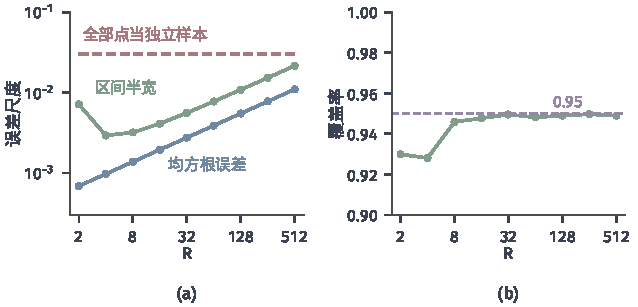
\includegraphics[width=108mm]{figures/07-probability/08-sampling-and-integration/matplotlib/budget-groups/figure.pdf}
  \caption{随机移位网格计算$\int_{0}^{1}\mathrm{e}^{u}\,\mathrm{d}u$，总点数$N=nR=1024$固定，横轴为组数$R$。(a)~蓝线为$R$组平均的均方根误差（精确公式），绿线为区间$\bar{Q}\pm t_{R-1}s_{Q}/\sqrt{R}$的平均半宽，红色虚线为把全部点当作独立样本时的半宽。(b)~该区间的覆盖率，紫色虚线为名义值$0.95$。(a)中的半宽与(b)均由$40000$次模拟得到（种子$3$）。}
  \label{fig:budget-groups}
\end{BookInlineFigure}

图中红色虚线是一个常见的错误：把全部$1024$个点的样本方差除以$1024$，得到半宽约$0.030$，比实际误差大一个数量级以上。这种做法在这里偏于保守，但它说明组内点不是独立样本，其样本方差与组平均的波动无关。对其他点集或被积函数，同样的错误也可能低估误差。综合两张图，总点数一定时，取十几到几十组通常是精度与误差估计可靠性之间的折中；若需要较准确的渐近区间，$R$还应更大，代价是单组的点数减少。

\section{方法选择}
\label{sec:budget-selection}

前三节给出了比较的尺子：误差口径、成本账和预算分配。还缺的是候选名单。一个方法能不能用，取决于目标分布和被积函数给了哪些可以计算的东西：能否计算分布函数的逆，能否逐点计算密度、只到一个常数因子还是完整归一化，能否对样本位置求导，是否知道某些辅助函数的精确期望。表~\ref{tab:budget-information}把前几章的方法按所需信息排列。

\begin{BookInlineTable}
  \centering
  \caption{可计算的信息与相应的方法}
  \label{tab:budget-information}
  \begin{tabular}{@{}p{44mm}p{62mm}@{}}
    \toprule
    可以计算的量 & 可用的方法 \\
    \midrule
    分位数函数 & 逆变换采样 \\
    混合成分或逐坐标条件分布 & 分步生成 \\
    有限包络常数下的密度比 & 拒绝采样 \\
    未归一化密度的比值 & MCMC，自归一化重要性采样 \\
    可采样且可计算密度的建议分布 & 重要性采样 \\
    期望已知的辅助函数 & 控制变量 \\
    精确的条件期望 & 条件期望降方差 \\
    层概率与层内条件抽样 & 分层采样 \\
    均匀输入下的生成映射 & 拉丁超立方，随机化准蒙特卡洛，对偶变量 \\
    被积函数对样本位置的导数 & 重参数化梯度 \\
    密度对参数的对数导数 & 得分函数梯度 \\
    \bottomrule
  \end{tabular}
\end{BookInlineTable}

名单只说明“可以用”，不说明“值得用”。一个方法可用而且理论上正确，并不意味着它在当前预算下比更朴素的方法有效。选择的依据始终是同一任务、同一误差口径下的总成本：先列出所有可用方案，再按第~\ref{sec:budget-costs}节的账估算每个方案的$\sigma^{2}c$和一次性开销，最后按预算决定。下面三小节分别对采样、方差控制和梯度估计做这件事。

\subsection{采样方法的选择}
\label{sec:budget-sampler-choice}

生成样本的方法大致按“需要的信息越多，结果越好”排列。直接生成（逆变换、分步生成）给出独立且精确服从目标的样本，每个样本成本固定；拒绝采样同样给出独立精确的样本，但每个输出平均要付出$M$个候选的成本；MCMC只需要未归一化密度的比值，代价是样本相关，而且要另行核验初值影响与探索范围。图~\ref{fig:budget-sampler-choice}把检查的顺序画成流程：从最强的信息问起，能用的第一个方法往往是成本最低的，但每个方法框右侧列出的量仍要逐项核对。

\begin{BookInlineFigure}
  \centering
  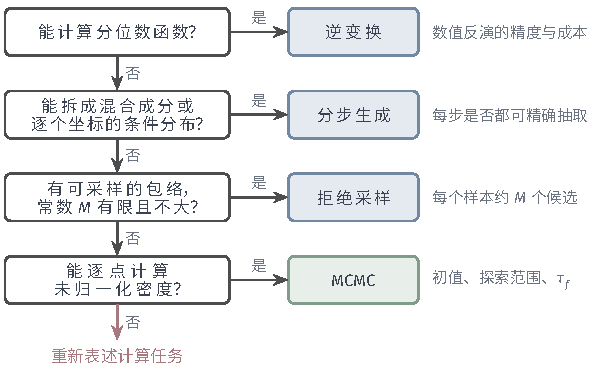
\includegraphics[width=101mm]{figures/07-probability/08-sampling-and-integration/tikz/budget-sampler-choice/figure.pdf}
  \caption{选择采样方法时依次检查的信息。左列从上到下要求的信息逐渐减少；每个方法框右侧是选定该方法后仍要比较的量：数值反演的精度、分步是否都能精确抽取、平均候选数$M$、链的初值影响与$\tau_{f}$。四项都不满足时（红色）需要改变计算任务的表述，例如换一个积分表示。}
  \label{fig:budget-sampler-choice}
\end{BookInlineFigure}

\paragraph{直接生成的数值精度}
分位数函数没有解析式时，逆变换要数值求解$F(x)=u$。用二分法在长度为$L$的区间上把$x$定位到容差$\eta$，需要约$\log_{2}(L/\eta)$次分布函数计算。容差带来一个确定性的偏差：输出不再精确服从$F$，而是服从相应的近似分布，第~\ref{chap:monte-carlo-integration-error}章说明这种偏差不随样本数减小。所以$\eta$要按最终的误差要求定：若$f$满足Lipschitz条件$\lvert f(x)-f(y)\rvert\le L_f\lvert x-y\rvert$，而数值反演把每个样本移动不超过$\eta$，则偏差不超过$L_f\eta$，取$L_f\eta$远小于$\varepsilon$即可，每个样本多付出的只是对数级的求值次数。

例如在长度$L=50$的区间上定位到$\eta=10^{-8}$，需要$\lceil\log_{2}(5\times10^{9})\rceil=33$次分布函数计算，比解析的逆变换贵几十倍，但仍可能比拒绝采样或MCMC便宜。分步生成要求每一步都能精确抽取；某一步只能近似时，整条生成链的偏差按同样方式核对。

\paragraph{拒绝采样的包络与尾部}
拒绝采样的成本由$M=\sup_{x}p(x)/q(x)$决定，而$M$有限要求包络在每个方向上的尾部不比目标轻。以$t_{3}$分布为目标，它的密度按$\lvert x\rvert^{-4}$衰减。用高斯包络$q_{1}=\mathcal{N}(0,2^{2})$时，比值
\[
  \frac{p(x)}{q_{1}(x)}\propto\Bigl(1+\frac{x^{2}}{3}\Bigr)^{-2}\mathrm{e}^{x^{2}/8}\to\infty,
\]
不存在有限的$M$；用Cauchy包络$q_{2}(x)=1/\bigl(\pi(1+x^{2})\bigr)$时比值有界，在$x=\pm1$处取最大值，网格计算得$M\approx1.30$。图~\ref{fig:budget-rejection-tails}画出这两种情形。

\begin{BookInlineFigure}
  \centering
  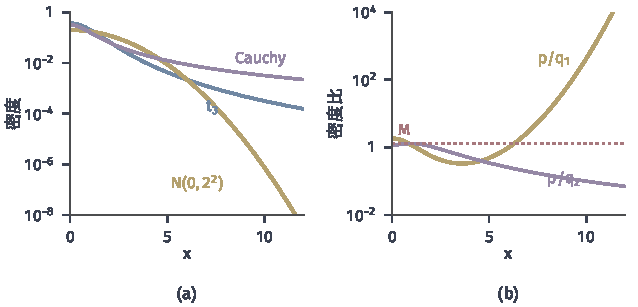
\includegraphics[width=108mm]{figures/07-probability/08-sampling-and-integration/matplotlib/budget-rejection-tails/figure.pdf}
  \caption{拒绝采样的包络必须覆盖目标的尾部。(a)~目标$t_{3}$（蓝）与两个包络的密度，对数纵轴：高斯$\mathcal{N}(0,2^{2})$（黄）在远处比目标轻得多，Cauchy（紫）比目标重。(b)~密度比$p/q$：对高斯包络无界，对Cauchy包络有界，红色点线为$M\approx1.30$。}
  \label{fig:budget-rejection-tails}
\end{BookInlineFigure}

若在高斯包络下强行取一个有限的“$M$”，例如只在$\lvert x\rvert\le6$上求最大值，算法仍然运行，但比值超过$M$的区域被系统地少接受，输出分布在尾部偏轻。这种错误不会使程序报错，样本的直方图在中心区域也与目标吻合；只有对依赖尾部的被积函数，例如$\mathbb{E}[X^{2}]$，偏差才显现出来。检查包络时，要对目标的支持和尾部给出解析的论证，而不是依赖样本。拒绝采样在高维的困难是另一回事：即使$M$有限，它也常随维数指数增长（第~\ref{chap:sample-generation}章），由式~\eqref{eq:budget-rejection-cost}，成本随之指数增长。

\paragraph{MCMC何时值得}
只有密度比可算时，MCMC往往是唯一的选择；但在直接生成或拒绝采样可用时，它通常不是最便宜的。图~\ref{fig:budget-sampler-costs}的双峰例子中，每个有效样本的成本是分步生成$4$、拒绝采样约$22$、最好的Metropolis约$52$。MCMC的优势在于每步只做局部的修改，在高维、各坐标强相关或只知道未归一化密度时，它的单步成本可以远低于任何直接生成方法。选择MCMC之后，比较的对象是转移核：步长、提议的形状、Gibbs与Metropolis--Hastings的组合等，比较的依据是针对所需被积函数的$c_{\mathrm{it}}\tau_{f}$，同时要有多次启动之类的检查（第~\ref{sec:budget-allocation}节）来确认链确实走遍了目标。

\subsection{方差控制方法的组合}
\label{sec:budget-vr-combination}

第~\ref{chap:variance-reduction}章的方法各自需要一种信息：重要性采样需要好的建议分布，控制变量需要期望已知且与$f$相关的辅助函数，条件期望降方差需要能精确计算的条件平均，分层需要层概率和层内条件抽样，对偶变量、拉丁超立方和随机化准蒙特卡洛需要从均匀输入出发的生成映射，共同随机数用于两个方案的差。它们可以叠加，例如先分层再在层内用对偶变量。叠加后的估计量是一个新的估计量，其期望、方差和成本都要重新计算，不能把各方法单独使用时的方差缩减倍数相乘或相加。

\paragraph{一个改进可能抵消另一个}
用$I=\mathbb{E}[\mathrm{e}^{U}]$、$U\sim\operatorname{Unif}(0,1)$比较几种组合，仍以每次计算$\mathrm{e}^{u}$为一个成本单位，辅助函数的计算视为免费。直接平均的单样本方差约为$0.2420$。对偶变量把$U$与$1-U$配成一对，每对的平均
\[
  g(U)=\frac{\mathrm{e}^{U}+\mathrm{e}^{1-U}}{2}
\]
要两次求值，按每次求值折算的方差约为$0.0078$。以$h(U)=U$作控制变量、取最优系数时，方差约为$0.0039$。

现在把两者叠加：先配对，再对配对后的估计用控制变量$U$。控制变量也要按同一种配对来算，即用$\bigl(U+(1-U)\bigr)/2$，而它恒等于$1/2$，没有任何波动可以利用。换一个角度，直接对$g(U)$与$U$求协方差：$g(u)=g(1-u)$关于$1/2$对称，而$U-1/2$反对称，于是
\[
  \operatorname{Cov}\bigl(g(U),U\bigr)=\mathbb{E}\bigl[g(U)(U-\tfrac12)\bigr]=\int_{0}^{1}g(u)\bigl(u-\tfrac12\bigr)\,\mathrm{d}u=0,
\]
因为把积分变量换成$1-u$后被积函数变号。对偶变量已经消去了$\mathrm{e}^{U}$中关于$1/2$的反对称部分，而$U$恰好只能解释这一部分。叠加的结果与单用对偶变量相同，比单用控制变量还差一倍。

反过来，若控制函数选在对偶变量留下的对称部分上，例如$h(U)=(U-\tfrac12)^{2}$，叠加后每次求值的方差降到约$2.2\times10^{-7}$。分层与对偶变量的叠加也类似：$4$层比例分层的方差约为$0.0165$，在每层内再配对后降到约$3.4\times10^{-5}$。图~\ref{fig:budget-vr-combos}把这些数并列，对数横轴上相差几个数量级。

\begin{BookInlineFigure}
  \centering
  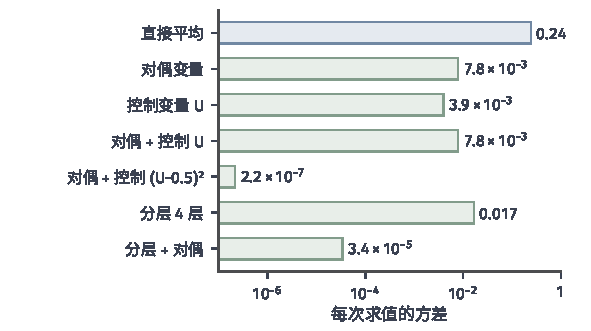
\includegraphics[width=100mm]{figures/07-probability/08-sampling-and-integration/matplotlib/budget-vr-combos/figure.pdf}
  \caption{计算$\mathbb{E}[\mathrm{e}^{U}]$时几种方差控制及其组合按每次求值折算的方差（数值积分精确计算，控制函数视为免费，控制系数取最优值）。蓝色为直接平均。“对偶 + 控制$U$”与单用对偶变量相同，因为配对后的控制量恒为$1/2$；控制函数改为对称的$(U-0.5)^{2}$后方差骤降。}
  \label{fig:budget-vr-combos}
\end{BookInlineFigure}

这组数字的教训是一般的：每种方法消去被积函数的某一部分波动，组合的效果取决于这些部分是否重叠。重叠时后一种方法无事可做，还白白付出成本；互补时效果可以远超任一方法单用。所以组合之后要按实际的估计量重新计算，第~\ref{chap:variance-reduction}章对单个方法证明的方差公式不能拼接使用。

\paragraph{高维均匀输入与变换后的函数}
拉丁超立方和随机化准蒙特卡洛作用在$[0,1)^{d}$的均匀输入上，被平均的是$F=f\circ T$，$T$是第~\ref{chap:sample-generation}章的生成映射。它们的改进依赖$F$的性质，而不是$f$的性质。拉丁超立方逐坐标均匀覆盖，对接近各坐标函数之和的$F$效果好，对主要由坐标间相互作用决定的$F$几乎无改进，有限样本下甚至可能不如独立抽样。随机化准蒙特卡洛的快速收敛要求$F$有一定的光滑性；若$T$是高斯的逆分布函数$\Phi^{-1}$，即使$f$光滑，$F$在立方体边界附近也无界，若$f$含示性函数，$F$在立方体内部有间断，两者都会使误差衰减变慢。选择这类方法时，要先检查变换后的函数，再按第~\ref{sec:budget-allocation}节选定$n$与$R$，误差只用组间方差估计。

\paragraph{两个方案的差}
比较两个方案的期望差$\mathbb{E}[A]-\mathbb{E}[B]$时，共同随机数用同一输入$U$生成$A(U)$与$B(U)$，由
\[
  \operatorname{Var}\bigl(A(U)-B(U)\bigr)=\operatorname{Var}(A)+\operatorname{Var}(B)-2\operatorname{Cov}\bigl(A(U),B(U)\bigr),
\]
正协方差越大，差的方差越小。与其他方法组合时要检查这种正协方差是否保留。若两个方案各自使用不同的重要性采样建议分布，同一个$U$在两边对应不同的样本位置，耦合可能失效；若两边都用逆变换且输出对输入单调同向，耦合通常最强。

用第~\ref{chap:variance-reduction}章的例子算一下：$A=\min\{X,1\}$，$X\sim\operatorname{Exp}(1)$；$B=\min\{Y,1\}$，$Y\sim\operatorname{Exp}(1.25)$；期望差约为$0.0613$。数值积分给出$\operatorname{Var}(A)\approx0.1289$、$\operatorname{Var}(B)\approx0.1291$。按差值的单对方差计，三种耦合方式的结果是
\[
  \underbrace{0.258}_{\text{独立输入}},\qquad\underbrace{0.0038}_{X,Y\text{用同一个}U},\qquad\underbrace{0.506}_{X\text{用}U,\ Y\text{用}1-U} .
\]
同向耦合把方差缩小约$68$倍；若误把对偶变量的反向配对用在差值上，协方差变负，方差反而比独立输入大近一倍。可见同一个“共用随机数”的操作，效果完全取决于两边输出对输入的单调方向。组合前后应各用一次小规模试运行，直接估计$\operatorname{Cov}(A,B)$，而不是假定它为正。

\subsection{梯度估计的选择}
\label{sec:budget-gradient-choice}

第~\ref{chap:expectation-gradient-estimation}章的三种表示分别依赖不同的条件。分布不随参数变化时，直接对被积函数求导；样本可写成$X=T_{\bm{\theta}}(\varepsilon)$且被积函数对样本位置可微时，用重参数化；能计算$\nabla_{\bm{\theta}}\ln p_{\bm{\theta}}$时，用得分函数，它不要求$f$对样本位置可微。离散样本空间上没有沿样本路径的导数，重参数化不能直接使用；状态数很少时还有一个更好的选择：直接求和。例如$X\sim\operatorname{Bern}(\theta)$时，$J(\theta)=\theta f(1)+(1-\theta)f(0)$，梯度$f(1)-f(0)$用两次求值就精确算出，没有任何随机误差。

条件都满足时，比较的依据仍是同一梯度任务下的偏差、方差与成本。不能预设重参数化总是方差更小，也不能预设得分函数总是更通用就更好。下面两个例子分别给出相反的结论。

\paragraph{被积函数振荡时}
设$X=\theta+\varepsilon$，$\varepsilon\sim\mathcal{N}(0,1)$，$f(x)=\sin(kx)$。由标准高斯的特征函数$\mathrm{e}^{-b^{2}/2}$，
\[
  J(\theta)=\sin(k\theta)\,\mathrm{e}^{-k^{2}/2},\qquad J'(\theta)=k\cos(k\theta)\,\mathrm{e}^{-k^{2}/2}.
\]
密度$\varphi(x-\theta)$的得分为$x-\theta$，在样本处等于$\varepsilon$，两种单样本估计分别是
\[
  \hat{g}_{\mathrm{R}}=k\cos\bigl(k(\theta+\varepsilon)\bigr),\qquad\hat{g}_{\mathrm{S}}=\sin\bigl(k(\theta+\varepsilon)\bigr)\,\varepsilon .
\]

用$\cos^{2}y=(1+\cos2y)/2$、$\sin^{2}y=(1-\cos2y)/2$及
\[
  \mathbb{E}\bigl[\cos(a+b\varepsilon)\bigr]=\cos a\,\mathrm{e}^{-b^{2}/2},\qquad\mathbb{E}\bigl[\varepsilon^{2}\cos(a+b\varepsilon)\bigr]=\cos a\,(1-b^{2})\,\mathrm{e}^{-b^{2}/2},
\]
两者的二阶矩分别为
\[
  \frac{k^{2}}{2}\bigl(1+\cos(2k\theta)\,\mathrm{e}^{-2k^{2}}\bigr),\qquad\frac12-\frac12\cos(2k\theta)\,(1-4k^{2})\,\mathrm{e}^{-2k^{2}} .
\]
减去梯度的平方即得方差。$k$较大时重参数化的方差约为$k^{2}/2$，得分函数的方差约为$1/2$：重参数化把$f$的导数带进估计，振荡越快，导数的幅度越大；得分函数只用到$f$的值，而$\lvert\sin\rvert\le1$。

图~\ref{fig:budget-gradient-variance}(a)取$\theta=0.3$，两条曲线在$k\approx1.09$相交。$k=0.5$时重参数化的方差约$0.0071$，得分函数约$0.31$，前者好四十多倍；$k=3$时前者约$4.50$，后者约$0.50$，后者好九倍。重参数化还要计算$f'$，每个样本的成本通常更高，所以$k$较大时得分函数在工作量归一化方差上的优势更明显。$2\times10^{6}$个样本的模拟（种子$1$）在$k=1$与$k=3$处与上面的公式相差不到$1\%$。

\begin{BookInlineFigure}
  \centering
  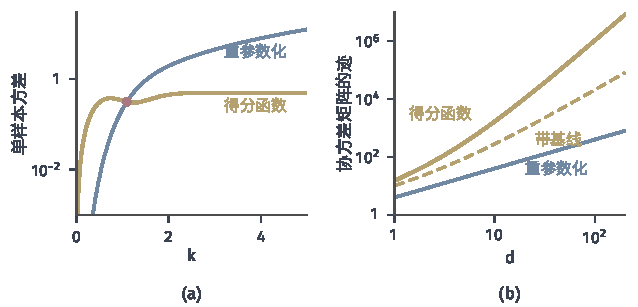
\includegraphics[width=108mm]{figures/07-probability/08-sampling-and-integration/matplotlib/budget-gradient-variance/figure.pdf}
  \caption{同一梯度任务下两种估计的单样本方差。(a)~$J(\theta)=\mathbb{E}[\sin(kX)]$，$X\sim\mathcal{N}(\theta,1)$，$\theta=0.3$：蓝线为重参数化，黄线为得分函数，红点为交点$k\approx1.09$。(b)~$J(\bm{\theta})=\mathbb{E}\lVert\bm{X}\rVert_2^{2}$，$\bm{X}\sim\mathcal{N}(\bm{\theta},\bm{I}_d)$，$\bm{\theta}=\bm{0}$：协方差矩阵的迹随维数$d$的变化，黄色虚线为得分函数减去基线$d$之后。}
  \label{fig:budget-gradient-variance}
\end{BookInlineFigure}

\paragraph{维数增大时}
设$\bm{X}=\bm{\theta}+\bm{\varepsilon}$，$\bm{\varepsilon}\sim\mathcal{N}(\bm{0},\bm{I}_d)$，$f(\bm{x})=\lVert\bm{x}\rVert_2^{2}$，在$\bm{\theta}=\bm{0}$处求梯度，真值为$\bm{0}$。

重参数化的估计是$2\bm{X}$，协方差矩阵为$4\bm{I}_d$，迹为$4d$。得分函数的估计是$\lVert\bm{X}\rVert_2^{2}\bm{X}$，由于真值为零，迹等于二阶矩$\mathbb{E}\lVert\bm{\varepsilon}\rVert_2^{6}$。$S=\lVert\bm{\varepsilon}\rVert_2^{2}$服从$\chi^{2}_{d}$，其各阶矩为
\[
  \mathbb{E}[S]=d,\qquad\mathbb{E}[S^{2}]=d(d+2),\qquad\mathbb{E}[S^{3}]=d(d+2)(d+4),
\]
于是
\[
  \operatorname{tr}\bm{\Sigma}_{\text{得分}}=\mathbb{E}\lVert\bm{\varepsilon}\rVert_2^{6}=d(d+2)(d+4).
\]
减去与样本独立的基线$b=\mathbb{E}\lVert\bm{X}\rVert_2^{2}=d$后，估计变为$(\lVert\bm{X}\rVert_2^{2}-d)\bm{X}$，其迹为
\[
  \begin{aligned}
    \mathbb{E}\bigl[(S-d)^{2}S\bigr]&=\mathbb{E}[S^{3}]-2d\,\mathbb{E}[S^{2}]+d^{2}\,\mathbb{E}[S]\\
    &=d(d+2)(d+4)-2d^{2}(d+2)+d^{3}=2d^{2}+8d .
  \end{aligned}
\]
基线把三次增长降成二次，但仍比重参数化的$4d$大约$d/2$倍。图~\ref{fig:budget-gradient-variance}(b)在对数坐标上显示了这三条曲线：$d=100$时分别为$400$、约$1.06\times10^{6}$与$20\,800$。这里重参数化每个样本要计算一次$\nabla f$，用反向自动求导时其成本是$f$的常数倍，与$d$无关，抵消不了$d/2$倍的方差差距。

\paragraph{可微性的条件}
重参数化的前提是把求导与求期望交换。$f$不连续时这一步可能失败而不报错。取$f(x)=\mathbf{1}_{\{x>0\}}$，$X=\theta+\varepsilon$，则$J(\theta)=\Phi(\theta)$，梯度为$\varphi(\theta)>0$；但对几乎每个$\varepsilon$，$\mathbf{1}_{\{\theta+\varepsilon>0\}}$在$\theta$附近是常数，路径导数为零，重参数化的估计恒为$0$。得分函数的估计$\mathbf{1}_{\{X>0\}}(X-\theta)$在这里无偏。所以选择重参数化之前，要先按第~\ref{chap:expectation-gradient-estimation}章检查交换条件，而不是看程序能否算出导数。

综合起来，梯度估计的选择依次回答四个问题：分布是否随参数变化；样本空间是否离散且小到可以直接求和；能否沿生成映射求导，且交换条件成立；能否计算得分。满足条件的估计都列出后，按式~\eqref{eq:budget-vector-mse}的迹或所需方向上的方差，乘以每个样本的成本来比较。参数怎样依据这些梯度更新，可参考\BookChapterRef{chap:stochastic-gradient-methods}{卷五第13章“随机梯度方法”}，那里梯度估计的方差直接影响步长的选择与收敛速度。

\section{试运行与停止}
\label{sec:budget-stopping}

前面的分配与选择都用到了事先不知道的量：单样本方差、成本、包络常数、$\tau_{f}$、建议分布的参数。它们只能由试运行估计。试运行的结果一旦用来做决定，后面的计算就依赖于这些随机的决定，原先对固定方法证明的结论是否还成立，需要重新检查。同样的问题出现在“何时停止”上：按事先固定的样本数停止，与看着结果决定何时停止，是两种不同的随机程序。

\paragraph{试运行与正式计算分开}
试运行的作用是估计成本、波动以及方法的参数，例如图~\ref{fig:budget-pilot-size}中的$\hat{\lambda}$、式~\eqref{eq:budget-neyman-cost}中的$\sigma_k$、图~\ref{fig:budget-sampler-costs}中的步长。正式计算用新的独立随机数。这样，给定试运行结果时，正式计算就是一个参数固定的普通方法，第~\ref{chap:monte-carlo-integration-error}章和第~\ref{chap:variance-reduction}章对固定方法证明的无偏性、方差公式和渐近区间都可以在条件意义下直接使用。

试运行的样本可不可以并入最终的平均？若试运行只是从固定的分布抽样且不参与任何选择，并入没有问题。若试运行被用来在几个方法中挑选，问题就来了：设对两个同样无偏的方法各做一次试运行，选估计方差较小的一个，再报告它在试运行中的估计。被选中的往往是试运行时“碰巧波动较小”的那一个，而对偏斜的被积函数，波动偏小常常伴随着均值偏小（漏掉了大的贡献），于是报告的数系统地偏低。最稳妥的做法是只把试运行用于决定，最终估计只用正式计算的样本；试运行所占的预算按式~\eqref{eq:budget-pilot-opt}本来就只是一小部分。

\paragraph{固定转移核与持续调参}
MCMC的步长、提议协方差等参数通常靠试运行调整。调整的依据应当是第~\ref{sec:budget-costs}节的$c_{\mathrm{it}}\tau_{f}$，而不只是接受率：图~\ref{fig:budget-sampler-costs}中接受率最高的$s=1$恰恰最贵。试运行结束后把参数固定，正式计算的链就是一条时间齐次的Markov链，转移核保持目标不变；但链是否从初值的影响中走出来、是否走遍目标、相关误差多大，仍要按第~\ref{chap:monte-carlo-integration-error}章逐项核对，参数选得好并不能免除这些检查。

一个诱人的做法是不停止调参：在正式计算中继续根据已走过的轨迹修改转移核。每个可能用到的核都以$\pi$为不变分布，看起来整体也应当正确。下面的例子说明这个推理不成立。状态空间为$\{1,2\}$，目标$\pi=(\tfrac12,\tfrac12)$。核$K_{A}$是恒等转移（停在原处），核$K_{B}$以概率$\tfrac12$去往每个状态，二者都保持$\pi$不变：
\[
  \pi K_{A}=\pi,\qquad\pi K_{B}=\bigl(\tfrac12,\tfrac12\bigr)=\pi .
\]
调整规则是：当前在状态$1$时用$K_{A}$，在状态$2$时用$K_{B}$。图~\ref{fig:budget-adaptive-trap}画出两个核及其组合。

\begin{BookInlineFigure}
  \centering
  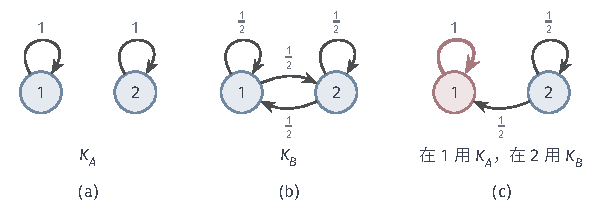
\includegraphics[width=101mm]{figures/07-probability/08-sampling-and-integration/tikz/budget-adaptive-trap/figure.pdf}
  \caption{每个核都保持目标不变，按轨迹选核却可能破坏它。状态空间$\{1,2\}$，目标$\pi=(\tfrac12,\tfrac12)$。(a)~$K_{A}$为恒等转移。(b)~$K_{B}$的每个转移概率都是$\tfrac12$。(c)~在状态$1$用$K_{A}$、在状态$2$用$K_{B}$的组合：状态$1$（红）成为吸收态。}
  \label{fig:budget-adaptive-trap}
\end{BookInlineFigure}

组合后的过程从状态$1$出发永远停在$1$，从状态$2$出发每步以$\tfrac12$的概率跳到$1$并从此停住。从$\pi$启动，$\mathbb{P}(X^{(0)}=2)=\tfrac12$，此后每步留在$2$的概率为$\tfrac12$，所以
\[
  \mathbb{P}\bigl(X^{(t)}=2\bigr)=\frac12\Bigl(\frac12\Bigr)^{t},\qquad\mathbb{P}\bigl(X^{(t)}=1\bigr)=1-2^{-(t+1)}\to1 .
\]
过程收敛到点质量$\delta_{1}$，而不是$\pi$。问题在于“用哪个核”依赖当前状态，组合起来的是另一个转移核，它不再保持$\pi$不变。不变性是对固定的核说的，不能由“每次所用的核都保持$\pi$”推出整体保持$\pi$。

持续调参并非不可行，但需要额外的理论。大致说，要求调整的幅度随时间趋于零，并且所用的核对目标的收敛速度有一致的控制，才能证明过程的边缘分布趋于$\pi$、平均满足大数律。这些条件涉及一般Markov链的遍历理论，证明较长，相关的收敛工具可参考\BookChapterRef{chap:discrete-time-stochastic-processes}{卷九第3章“离散时间随机过程”}。本卷采用更简单的做法：试运行中调参，正式计算中固定。

\paragraph{经验稳定的局限}
试运行和停止判断都要看结果是否“稳定”，但有限记录上的稳定不能证明正确。下面三种现象都会让运行均值在错误的值附近显得平稳。

第一种是稀有的大贡献。若对积分起主要作用的区域概率很小，有限的试运行可能一个样本也没有落进去，估计的方差为零，一切看起来都很精确。图~\ref{fig:budget-pilot-size}的例子之所以平稳，是因为$q_{0}=\operatorname{Exp}(1/2)$落入尾部的概率是$\mathrm{e}^{-2}\approx0.135$；若试运行直接从$\operatorname{Exp}(1)$抽样，这个概率只有$0.018$，$n_{0}=20$时有约$69\%$的试运行完全看不到尾部。

第二种是权重集中。仍算$I=\mathbb{P}(X>4)$，但用尾部比目标还轻的建议分布$q=\operatorname{Exp}(2.2)$。权重$w(y)=\mathrm{e}^{-y}/(2.2\,\mathrm{e}^{-2.2y})$在尾部指数增长，加权变量在$q$下的二阶矩为
\[
  \int_{4}^{\infty}\frac{\mathrm{e}^{-2y}}{2.2\,\mathrm{e}^{-2.2y}}\,\mathrm{d}y=\frac{1}{2.2}\int_{4}^{\infty}\mathrm{e}^{0.2y}\,\mathrm{d}y=\infty,
\]
估计无偏而方差无穷。图~\ref{fig:budget-weight-instability}画出三次独立运行：每次在前几千个样本内都没有命中尾部，估计为零；命中后估计跳起，之后每隔一段又被一个更大的权重抬升。$10^{6}$个样本后三次的估计约为$0.0149$、$0.0164$、$0.0163$，都低于$I\approx0.0183$。右图是最大的一项在累计和中的占比：它长时间接近$1$，说明整个估计由一两个样本决定。

\begin{BookInlineFigure}
  \centering
  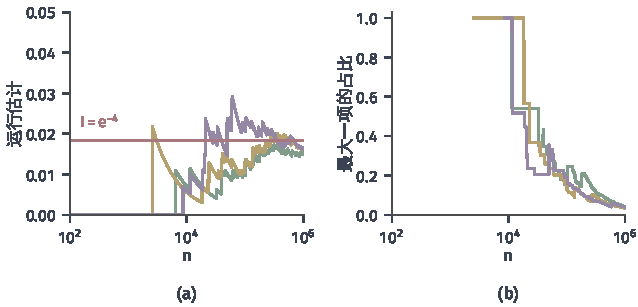
\includegraphics[width=108mm]{figures/07-probability/08-sampling-and-integration/matplotlib/budget-weight-instability/figure.pdf}
  \caption{建议分布尾部过轻时的重要性采样：目标$I=\mathbb{P}(X>4)$，$X\sim\operatorname{Exp}(1)$，从$\operatorname{Exp}(2.2)$抽样，加权变量方差无穷。三种颜色是三次独立运行（种子$11$、$12$、$13$）。(a)~运行估计，红线为真值。(b)~累计和中最大一项所占的比例。}
  \label{fig:budget-weight-instability}
\end{BookInlineFigure}

第三种是链之间的分歧。图~\ref{fig:budget-multistart}中每条链的运行均值都在某个值附近平稳下来，只有并排比较多条从不同初值出发的链，才看得出它们停在不同的地方。

这三种现象对应三种检查：对被积函数与建议分布的尾部做解析的矩估计，监视最大权重的占比，比较多条独立启动的链。它们能发现问题，但都不能证明没有问题：若所有链都错过了同一个峰，或所有试运行都没有触及同一个稀有区域，检查也全部通过。经验检查只能补充理论条件，不能代替它。

\paragraph{固定样本数与数据依赖的停止}
最常见的停止方式是看着误差估计做决定：每增加一些样本就计算一次$z\,s_n/\sqrt{n}$，一旦它小于容差$\varepsilon$就停止，报告$\bar{X}_n\pm z\,s_n/\sqrt{n}$。称这类规则为\term{序贯停止规则}（sequential stopping rule），停止时的样本数$N_{\varepsilon}$是随机的，依赖于样本本身。固定样本数的中心极限定理说的是$n$不随数据变化的情形，不能直接搬到$N_{\varepsilon}$上。

机制在偏斜分布上最清楚。设$f(U)=U^{-1/3}$，即$X$服从$[1,\infty)$上指数为$3$的Pareto分布，$I=1.5$，$\sigma^{2}=0.75$，右尾较重。一段样本恰好没有出现大值时，$s_n$偏小，均值也偏小；停止规则偏偏在这种时候触发，于是停下来时的估计系统地偏低，区间又偏窄。取$z=1.96$、最少$10$个样本、每增加一个样本检查一次，$20000$次模拟（种子$5$）的结果如图~\ref{fig:budget-sequential-coverage}。$\varepsilon=0.1$时，用真实$\sigma^{2}$定出的固定样本数$n=\lceil1.96^{2}\times0.75/0.01\rceil=289$，区间覆盖率约$0.925$；序贯规则平均只用了约$174$个样本就停止，覆盖率只有约$0.77$。

\begin{BookInlineFigure}
  \centering
  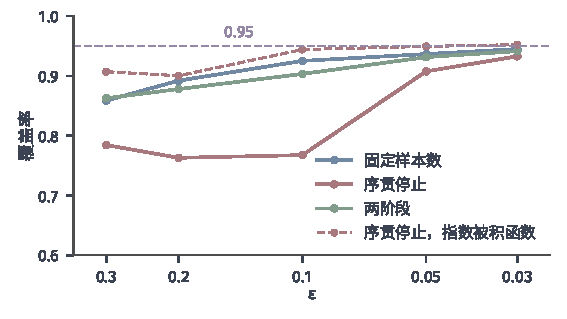
\includegraphics[width=96mm]{figures/07-probability/08-sampling-and-integration/matplotlib/budget-sequential-coverage/figure.pdf}
  \caption{名义$95\%$区间在三种停止方式下的实际覆盖率，横轴为目标半宽$\varepsilon$（向右减小）。实线为偏斜的被积函数$U^{-1/3}$（$I=1.5$，$\sigma^{2}=0.75$）：蓝线用真实方差定出固定样本数，红线在半宽首次小于$\varepsilon$时停止（最少$10$个样本），绿线先用$30$个独立试运行样本估计方差再定样本数。红色虚线为序贯停止用于$\mathrm{e}^{U}$的情形。每点$20000$次模拟（种子$5$）。}
  \label{fig:budget-sequential-coverage}
\end{BookInlineFigure}

$\varepsilon$变小时三条实线都向$0.95$靠拢：$\varepsilon=0.03$时固定样本数、两阶段与序贯规则的覆盖率分别约为$0.945$、$0.941$、$0.933$。对较对称的$\mathrm{e}^{U}$，序贯规则在$\varepsilon=0.1$时已有约$0.944$。这与一个渐近结论相符：若$0<\sigma^{2}<\infty$，并且停止规则要求的最少样本数随$\varepsilon\to0$趋于无穷（或在判据中加入防止过早停止的修正项），则$\varepsilon\to0$时覆盖率趋于名义值。它的证明需要随机样本数下的中心极限定理，篇幅较长，这里只说明其含义：数据依赖的停止只在误差要求足够严、停止时样本足够多时才近似可靠，对给定的有限$\varepsilon$没有保证。

既想依据数据定样本数、又要保留固定样本数的保证，可以把决定和估计分开，称为\term{两阶段方法}（two-stage procedure）：先用独立的试运行估计方差，据此定出正式样本数，再用新样本计算。

\begin{lemma}
\label{lem:budget-two-stage}
设试运行样本$\bm{Y}$与正式样本$X_1,X_2,\dots$相互独立，$X_i$独立同分布，$\mathbb{E}[X_i]=I$，$\operatorname{Var}(X_i)=\sigma^{2}<\infty$。正式样本数$N$是$\bm{Y}$的函数，取正整数值。令$\hat{I}=N^{-1}\sum_{i=1}^{N}X_i$，则
\begin{equation}
  \mathbb{E}\bigl[\hat{I}\mid\bm{Y}\bigr]=I,\qquad\operatorname{Var}\bigl(\hat{I}\mid\bm{Y}\bigr)=\frac{\sigma^{2}}{N},\qquad\operatorname{Var}(\hat{I})=\sigma^{2}\,\mathbb{E}\Bigl[\frac1N\Bigr].
  \label{eq:budget-two-stage}
\end{equation}
\end{lemma}

\begin{proof}
给定$\bm{Y}=\bm{y}$时$N=n(\bm{y})$是确定的正整数。由独立性，在这一条件下$X_1,X_2,\dots$的联合分布不变，仍独立同分布、均值$I$、方差$\sigma^{2}$。于是$n(\bm{y})$个样本的平均的条件期望为$I$，条件方差为$\sigma^{2}/n(\bm{y})$，这就是前两个等式。

由全期望公式，
\[
  \mathbb{E}[\hat{I}]=\mathbb{E}\bigl[\mathbb{E}[\hat{I}\mid\bm{Y}]\bigr]=I .
\]
由全方差公式，
\[
  \operatorname{Var}(\hat{I})=\mathbb{E}\bigl[\operatorname{Var}(\hat{I}\mid\bm{Y})\bigr]+\operatorname{Var}\bigl(\mathbb{E}[\hat{I}\mid\bm{Y}]\bigr)=\mathbb{E}\Bigl[\frac{\sigma^{2}}{N}\Bigr]+\operatorname{Var}(I)=\sigma^{2}\,\mathbb{E}\Bigl[\frac1N\Bigr],
\]
因为常数$I$的方差为零。
\end{proof}

引理的要点是$N$只依赖试运行。条件在试运行上，正式计算就是固定样本数的计算，固定样本数的渐近区间在条件意义下适用；$N$越大，条件覆盖率越接近名义值。图~\ref{fig:budget-sequential-coverage}的绿线用$30$个试运行样本的标准差$s_{0}$定出
\[
  N=\max\bigl\{30,\ \lceil z^{2}s_{0}^{2}/\varepsilon^{2}\rceil\bigr\},
\]
其覆盖率略低于用真实方差的蓝线（$\varepsilon=0.1$时约$0.903$对$0.925$），而明显高于序贯规则。差距来自试运行：$s_{0}$偏小时$N$偏小，最终区间可能比$\varepsilon$宽，也就是精度没有达标；但估计本身在条件意义下仍然无偏，不再出现序贯规则那种系统偏低。若$\bm{Y}$与正式样本不独立，例如把试运行样本并入最终平均，引理的条件就不满足。

用积分$\mathrm{e}-1$走一遍两阶段方法，取$\varepsilon=0.01$、$z=1.96$，随机数种子固定为$2026$。$30$个试运行样本的标准差为$s_{0}\approx0.426$，比真实的$\sigma\approx0.492$偏小，于是
\[
  N=\Bigl\lceil\frac{1.96^{2}\times0.426^{2}}{10^{-4}}\Bigr\rceil=6984,
\]
少于用真实方差算出的约$9300$。用新的$6984$个样本得到均值约$1.7290$，标准差约$0.493$，区间半宽为
\[
  1.96\times\frac{0.493}{\sqrt{6984}}\approx0.0116 .
\]
半宽超过了要求的$0.01$，这是试运行低估方差的后果；但这个区间如实反映了正式样本的波动，其下端约为$1.7174$，覆盖了$\mathrm{e}-1\approx1.7183$。若精度必须达标，可以把这次结果当作新的试运行，再定一次样本数，并仍用新样本计算。

最后，“预算用完就停”是固定预算的停止，样本数不依赖于样本的取值，固定样本数的结论适用。若每个样本的成本本身随机（例如拒绝采样的候选数），按预算停止时的样本数也随机，但它只依赖成本，不依赖被积函数的取值；拒绝采样中接受与否与被接受样本的取值独立，这种停止不会造成上面那种偏差。

\section{本章小结}
\label{sec:budget-summary}

本章把采样生成、误差分析、方差控制与梯度表示放到同一本账上，回答“给定任务和预算，怎样安排一次随机计算”。回到章首的问题：计算$I=\mathbb{P}(X>4)$，要求$95\%$把握下相对误差不超过$10\%$。$I\approx0.0183$离零较远，相对要求有意义，按式~\eqref{eq:budget-mixed-tolerance}给一个绝对下限以防目标接近零即可。直接平均约需$20\,600$个样本；先用几十个试运行样本拟合$\operatorname{Exp}(\lambda)$建议分布，再做重要性采样，约需$1990$个正式样本，成本约$3000$。两者都在$10^{5}$的预算之内，后者约省$85\%$；正式样本数按两阶段方法由试运行确定，最终估计只用正式样本。

\paragraph{误差与成本的口径}
误差要求先要说清是均方误差、指定概率下的绝对误差，还是相对误差；目标可能为零时用混合容差。无偏方法之间比较工作量归一化方差$\sigma^{2}c$，它在固定预算与固定精度两种提法下给出同一排序；有偏方法还要选择控制偏差的参数，近似链的例子中最优安排使均方根误差只按$B^{-1/3}$下降。成本要计入被拒绝的候选、矩阵分解与试运行等一次性开销，以及链的初始化；相关链按有效样本计成本，而有效样本数依赖被积函数，抽稀只节省存储。

\paragraph{预算的分配}
试运行的最优规模按$\sqrt{C}$增长，占预算的比例随预算增大而缩小，最终误差对它的具体取值通常不敏感。分层的最优分配在考虑成本时为$n_k\propto p_k\sigma_k/\sqrt{c_k}$。对单峰且混合良好的链，一条长链的均方误差最小，多条短链各自带着初值偏差；多次启动的价值在于暴露链没有走遍目标。成组随机化中，组内点数$n$决定精度，组数$R$决定误差估计的可靠性，不能把全部点当作独立样本估计误差。

\paragraph{方法的选择}
可用的方法由可计算的信息决定：分位数、条件分布、有限包络、密度比、期望已知的辅助函数、可微的生成映射或得分。在可用的方法之间，以同一任务的总成本比较：一维双峰例子中直接生成比最好的Metropolis便宜十几倍；方差控制的组合要重新计算，对偶变量之后再用控制变量$U$毫无收益，而换成对称的控制函数则收益巨大；梯度估计没有普遍的优劣，被积函数振荡时得分函数方差小，维数高时重参数化方差小，被积函数不连续时重参数化可能静默地给出错误结果。

\paragraph{试运行与停止的条件}
试运行只用于决定，正式计算用新的随机数，固定方法的结论才在条件意义下适用。MCMC在试运行中调参、正式计算中固定转移核；按轨迹持续换核，即使每个核都保持目标不变，整体也可能收敛到错误的分布。稀有贡献、权重集中与链间分歧都能让有限记录显得平稳，经验检查只能发现问题，不能证明正确。依据误差估计决定何时停止会使偏斜被积函数的区间系统性地失效，只在要求足够严时渐近可靠；把定样本数与计算估计分开的两阶段方法保留了固定样本数的结论。

最终报告一次随机计算，应分别给出计算偏差（及其来源，如近似生成或初值）、随机波动（及其估计方式和所依据的条件）以及实际成本。这里的“精度”是对一个确定的数做随机计算时的精度：分布已知、积分待算，随机性完全来自我们所用的随机数，可以通过增加计算来减小。它与由有限数据推断未知总体时的精度是两回事，后者的误差来自数据本身，加大计算量无法消除，相应的理论见\BookChapterRef{chap:parametric-statistical-inference}{卷八第1章“参数化统计推断”}。


